\باب{کثیر المتغیر تفاعل اور جزوی تفرقات}
\موٹا{جائزہ}\\
سائنس میں دو یا دو سے زائد غیر تابع  متغیرات کے تفاعل    ایک متغیر کے تفاعل سے زیادہ کثرت سے پائے جاتے ہیں اور ان کی علم   احصاء  زیادہ  عمدہ   ہوتی  ہے۔زیادہ متغیرات ایک دوسرے پر زیادہ طریقوں سے اثر انداز ہو سکتے ہیں جس کی بنا ان کے تفرقات    مختلف اور زیادہ دلچسپ  صورتیں اختیار  کر سکتے ہیں۔ ان کے تکملات  زیادہ اقسام کے عملی  مسائل میں کام آتے ہیں۔ احتمال،  سیالی حرکیات، اور برقیات، وغیرہ،    پر غور کے دوران  ایک سے زائد متغیرات  کے تفاعل قدرتی طور پر رونما ہوتے ہیں۔ان تفاعل کی  ریاضیات، سائنس کی عظیم  کامیابیوں میں  سے ایک ہے۔


\حصہ{کثیر متغیرات کے تفاعل}
کئی تفاعل ایک سے زائد متغیرات کے تابع  ہوتے ہیں۔دائری نلکی کا حجم،  اس    کے رداس اور قد سے،   تفاعل  \عددی{H=\pi r^2h}   دیتا ہے۔ مستوی \عددی{xy} میں نقطہ \عددی{N(x,y)} کے دو محدد سے،   قطع مکافی   \عددی{z=x^2+y^2}  کا قد  تفاعل \عددی{f(x,y)=x^2+y^2} دیتا ہے۔اس حصہ میں ہم ایک سے زیادہ متغیرات کے تابع تفاعل متعارف کرتے ہیں  اور ان کو ترسیم کرنے کے طریقوں پر غور کرتے ہیں۔

\جزوحصہء{تفاعل اور متغیرات} 
کثیر غیر تابع حقیقی متغیرات  کے حقیقی قیمت تفاعل کی تعریف  بالکل واحد متغیر کے تفاعل کی طرح کی جاتی ہے۔ان کے وقفے  حقیقی   (تین، چار، وغیرہ)    اعداد کے  مرتب جوڑی  کے سلسلے ہوں گے اور ان  کی  سعت  ، اس طرح  کے حقیقی اعداد کے سلسلے ہوں گے جن کے ساتھ ہم کام کرتے آ رہے ہیں۔

\ابتدا{تعریفات}
فرض کریں \عددی{n} عدد حقیقی اعداد \عددی{x_1,x_2,\cdots,x_n} کا سلسلہ \عددی{D} ہے۔  تب \عددی{D} پر \اصطلاح{حقیقی قیمت تفاعل}\فرہنگ{تفاعل!حقیقی قیمت}\حاشیہب{real valued function}\فرہنگ{function!real valued} \عددی{f} سے مراد وہ قاعدہ ہے جو \عددی{D} کے ہر رکن کو حقیقی عدد
\begin{align*}
w=f(x_1,x_2,\cdots,x_n)
\end{align*}
مختص کرتا ہو۔سلسلہ \عددی{D} اس تفاعل کا \اصطلاح{دائرہ کار}\فرہنگ{دائرہ کار}\حاشیہب{domain}\فرہنگ{domain} ہو گا۔  تفاعل  \عددی{f} کی  \عددی{w} قیمتوں کا سلسلہ  \عددی{f} کی \اصطلاح{سعت}\فرہنگ{سعت}\حاشیہب{range}\فرہنگ{range} ہو گی۔ علامت \عددی{w} تفاعل \عددی{f} کا \اصطلاح{تابع متغیر}\فرہنگ{متغیر!تابع}\حاشیہب{dependent variable}\فرہنگ{variable!dependent} ہو گا اور \عددی{f} کو  \عددی{n}  \اصطلاح{غیر تابع متغیرات}\فرہنگ{متغیر!غیر تابع}\حاشیہب{independent variable}\فرہنگ{variable!independent} \عددی{x_1} تا \عددی{x_n}   کا تفاعل کہتے ہیں۔ ہم  ان \عددی{x} کو تفاعل کے \اصطلاح{داخلی متغیرات}\فرہنگ{متغیر!داخلی}\حاشیہب{input variable}\فرہنگ{variable!input} اور \عددی{w} کو تفاعل کا \اصطلاح{خارجی متغیر}\فرہنگ{متغیر!خارجی}\حاشیہب{output variable}\فرہنگ{variable!output}  بھی کہتے ہیں۔
\انتہا{تعریفات}
%==================

اگر \عددی{f} دو غیر تابع متغیرات کا تفاعل ہو تب عموماً ہم  ان غیر تابع متغیرات کو \عددی{x} اور \عددی{y} کہتے ہیں اور \عددی{f} کے دائرہ کار  کو مستوی \عددی{xy} میں ایک خطہ تصور کرتے ہیں۔ اگر \عددی{f} تین غیر تابع متغیرات کا تفاعل ہو تب ہم  ان متغیرات کو \عددی{x}، \عددی{y} اور \عددی{z} کہتے ہیں اور تفاعل کے  دائرہ کار کو فضا میں ایک خطہ تصور کرتے ہیں۔

عملی استعمال میں ہم  وہ حروف استعمال کرتے ہیں جو ہمیں ان چیزوں  کی یاد  دلا سکیں جن کے لئے یہ متغیرات استعمال  کیے گئے ہوں۔ یہ  کہنے  کی خاطر کہ دائری نلکی کا حجم اس کے رداس \عددی{r}  اور قد \عددی{h}   کا تفاعل ہو گا، ہم \عددی{H=f(r,h)} لکھ سکتے ہیں۔بالخصوص  ہم \عددی{f(r,h)} کی جگہ وہ کلیہ استعمال کر سکتے ہیں جو \عددی{r} اور \عددی{h} کی قیمتوں سے \عددی{H} کی  قیمت دیتا ہو، یعنی ہم  \عددی{H=\pi r^2h} لکھ سکتے ہیں۔دونوں صورتوں میں \عددی{r} اور \عددی{h} غیر تابع متغیرات ہوں گے اور \عددی{H} تابع متغیر ہو گا۔

ہمیشہ کی طرح،ہم  تفاعل کی تعریفی کلیہ میں غیر تابع متغیرات کی قیمتیں پر کر  کے مطابقتی تابع متغیر کی قیمت حاصل کرتے ہیں۔

\ابتدا{مثال}
نقطہ \عددی{(3,0,4)} پر تفاعل \عددی{f(x,y,z)=\sqrt{x^2+y^2+z^2}} کی قیمت درج ذیل ہو گی۔
\begin{align*}
f(3,0,4)=\sqrt{(3)^2+(0)^2+(4)^2}=\sqrt{25}=5
\end{align*}
\انتہا{مثال}
%===============
\جزوحصہء{وقفے}
ایک سے زیادہ متغیرات کے تفاعل  کی تعریف  میں، ہمیشہ کی طرح، ہم  ان مداخل کو  شامل نہیں  کرتے ہیں  جو مخلوط اعداد دیتے ہوں یا جن کی وجہ سے   تقسیم صفر  کا عمل  پیدا ہوتا ہو۔یوں \عددی{f(x,y)=\sqrt{y-x^2}} میں \عددی{y} کی قیمت \عددی{x^2} کی قیمت سے کم نہیں ہو سکتی ہے اور \عددی{f(x,y)=\tfrac{1}{xy}} میں \عددی{xy} کی قیمت صفر نہیں ہو سکتی ہے۔ان شرائط کو مطمئن کرتے ہوئے، تفاعل کے  دائرہ کار سے مراد  وہ بڑے سے بڑا سلسلہ ہو گا جس پر تفاعل کا  تعریفی قاعدہ حقیقی اعداد  پیدا کرتا ہو۔ 

\ابتدا{مثال}\ترچھا{دو متغیرات کے تفاعل}\\
\begin{center}
\renewcommand{\arraystretch}{1.2} 
\begin{tabular}{LLL}
\multicolumn{1}{C}{\text{\RL{تفاعل}}}&\text{\RL{دائرہ کار}}&\multicolumn{1}{C}{\text{\RL{سعت}}}\\
\midrule
w=\sqrt{y-x^2}&y\ge x^2&[0,\infty)\\
w=\tfrac{1}{xy}&xy\ne 0&(-\infty,0)\cup(0,\infty)\\
w=\sin xy&\text{\RL{پورا مستوی}}&[-1,1]
\end{tabular}
\end{center}
\انتہا{مثال}
%===============
\ابتدا{مثال}\ترچھا{تین متغیرات کے  تفاعل}\\
\begin{center}
\renewcommand{\arraystretch}{1.2} 
\begin{tabular}{LLL}
\multicolumn{1}{C}{\text{\RL{تفاعل}}}&\multicolumn{1}{C}{\text{\RL{دائرہ کار}}}&\multicolumn{1}{C}{\text{\RL{سعت}}}\\
\midrule
w=\sqrt{x^2+y^2+z^2}&\text{\RL{پوری فضا}}&[0,\infty)\\
w=\dfrac{1}{x^2+y^2+z^2}&(x,y,z)\ne (0,0,0)&(0,\infty)\\
w=xy\ln z&\text{\RL{نصف فضا z>0}}&(-\infty,\infty)
\end{tabular}
\end{center}
\انتہا{مثال}
%===========
بالکل حقیقی لکیر کے وقفوں  پر معین تفاعل کے دائرہ کار کی طرح، مستوی  کے حصوں پر معین تفاعل کے دائرہ کار کے اندرونی نقطے اور  سرحدی نقطے  ہو سکتے ہیں۔
\begin{figure}
\centering
\begin{subfigure}{0.45\textwidth}
\centering
\begin{tikzpicture}[scale=0.75]
\draw[smooth cycle,fill=llgray]plot coordinates {(0,0)(1,-2)(2,-1.5)(3,-2)(5,-1)(4.5,0)(5,1)(2,2)(1,1.5)};
\draw[dashed,fill=lgray](3,-0.5)node[circ]{}node[pin={[pin edge=solid]135:{$(x_0,y_0)$}}]{} circle (0.5);
\draw(1,-1)node[]{$R$};
\end{tikzpicture}
\caption{اندرونی نقطہ}
\end{subfigure}\hfill
\begin{subfigure}{0.45\textwidth}
\centering
\begin{tikzpicture}[scale=0.75]
\draw[name path=kout,smooth cycle,fill=llgray]plot coordinates {(0,0)(1,-2)(2,-1.5)(3,-2)(5,-1)(4.5,0)(5,1)(2,2)(1,1.5)};
\draw(1,-1)node[]{$R$};
\begin{scope}
\path[clip,smooth cycle]plot coordinates {(0,0)(1,-2)(2,-1.5)(3,-2)(5,-1)(4.5,0)(5,1)(2,2)(1,1.5)};
\fill[lgray](3,-2) circle (0.5);
\end{scope}
\draw[dashed,name path=kin](3,-2)node[circ]{}node[pin={[pin edge=solid,above]70:{$(x_0,y_0)$}}]{} circle (0.5);
\end{tikzpicture}
\caption{سرحدی  نقطہ}
\end{subfigure}
\caption{مستوی خطہ \عددی{R}  کا اندرونی نقطہ اور سرحدی نقطہ۔اندرونی نقطہ لازماً \عددی{R} کا حصہ ہو گا جبکہ ضروری نہیں کہ سرحدی نقطہ \عددی{} کا حصہ ہو۔}
\label{شکل_کثیرالمتغیر_اندرونی_سرحدی_نقاط}
\end{figure}

\ابتدا{تعریفات}
مستوی \عددی{xy} میں خطہ (سلسلہ) \عددی{R}  میں نقطہ \عددی{(x_0,y_0)}  تب \عددی{R} کا \اصطلاح{اندرونی نقطہ}\فرہنگ{نقطہ!اندرونی}\حاشیہب{interior point}\فرہنگ{point!interior} ہو گا جب  یہ اس قرص کا مرکز  ہو جو مکمل طور پر \عددی{R} میں پایا جاتا ہو (شکل \حوالہ{شکل_کثیرالمتغیر_اندرونی_سرحدی_نقاط})۔  نقطہ \عددی{(x_0,y_0)} تب \عددی{R} کا  \اصطلاح{سرحدی نقطہ}\فرہنگ{نقطہ!سرحدی}\حاشیہب{boundary point}\فرہنگ{point!boundary} ہو گا جب ہر اس  قرص  میں، جس کا مرکز \عددی{(x_0,y_0)} ہو ،  \عددی{R} کے بیرونی  اور \عددی{R} کے اندرونی نقطے پائے جاتے ہوں۔(ضروری نہیں کہ سرحدی نقطہ ازخود \عددی{R} میں شامل  ہو۔ )

ایک خطہ کے اندرونی نقطے، بطور ایک سلسلہ، اس خطہ  کی\اصطلاح{ اندرون}\فرہنگ{اندرون}\حاشیہب{interior}\فرہنگ{interior} ہوں گے۔ اس خطہ کے سرحدی نقطے اس کی \اصطلاح{سرحد}\فرہنگ{سرحد}\حاشیہب{boundary}\فرہنگ{boundary}  ہیں۔ایسا خطہ  جو مکمل طور پر اندرونی نقطوں پر مشتمل ہو \اصطلاح{کھلا}\فرہنگ{کھلا}\حاشیہب{open}\فرہنگ{open} خطہ کہلاتا ہے۔ ایسا خطہ جس میں  اس کے تمام سرحدی نقطے شامل ہوں \اصطلاح{بند}\فرہنگ{بند}\حاشیہب{closed}\فرہنگ{closed} خطہ کہلاتا ہے۔ 
\انتہا{تعریفات}
%===================
\begin{figure}
\centering
\begin{subfigure}{0.30\textwidth}
\centering
\begin{tikzpicture}
\draw(0,0)node[below left]{$O$};
\fill[llgray](0,0) circle (1);
\draw[dashed,fill=lgray](0.4,0.4)node[circ]{} circle (0.25);
\draw[-latex](-1.5,0)--(1.5,0)node[right]{$x$};
\draw[-latex](0,-1.25)--(0,1.5)node[left]{$y$};
\end{tikzpicture}
\caption{
\عددی{\{(x,y)|x^2+y^2<1\}}\\
کھلا قرص۔ ہر نقطہ اندرونی نقطہ ہے۔
}
\end{subfigure}\hfill
\begin{subfigure}{0.30\textwidth}
\centering
\begin{tikzpicture}
\draw(0,0)node[below left]{$O$};
\begin{scope}
\draw[clip](0,0) circle (1);
\fill[lgray](45:1) circle (0.25);
\end{scope}
\draw[dashed](45:1)node[circ]{} circle (0.25);
\draw[-latex](-1.5,0)--(1.5,0)node[right]{$x$};
\draw[-latex](0,-1.25)--(0,1.5)node[left]{$y$};
\end{tikzpicture}
\caption{
\عددی{\{(x,y)|x^2+y^2=1\}}\\
اکائی قرص کی  سرحد۔ (اکائی دائرہ۔)
}
\end{subfigure}\hfill
\begin{subfigure}{0.30\textwidth}
\centering
\begin{tikzpicture}
\draw(0,0)node[below left]{$O$};
\draw[fill=llgray](0,0) circle (1);
\draw[-latex](-1.5,0)--(1.5,0)node[right]{$x$};
\draw[-latex](0,-1.25)--(0,1.5)node[left]{$y$};
\end{tikzpicture}
\caption{
\عددی{\{(x,y)|x^2+y^2\le 1\}}\\
بند اکائی قرص۔تمام سرحدی نقطے اس میں شامل ہیں۔
}
\end{subfigure}
\caption{مستوی میں اکائی قرص کے اندرونی نقطے اور سرحدی نقطے۔}
\label{شکل_کثیرالمتغیر_اکائی_قرص_اندرونی_سرحدی}
\end{figure}

حقیقی اعداد کے وقفوں کی طرح، مستوی میں بعض خطے نا کھلا اور نا ہی بند ہوتے ہیں۔ شکل \حوالہ{شکل_کثیرالمتغیر_اکائی_قرص_اندرونی_سرحدی} کے کھلا قرص   میں چند،   نا کہ  تمام،    سرحدی نقطے شامل کرنے سے ایسا خطہ حاصل ہو گا جو نا کھلا ہو گا اور نا ہی بند ہو گا۔اس میں شامل سرحدی نقطے اس کو کھلا وقفہ بننے  سے روکتے  ہیں جبکہ اس میں نا  شامل سرحدی نقطے اس کو  بند  خطہ بننے سے روکتے ہیں۔

\ابتدا{تعریف}
مستوی میں  مقررہ رداس کے قرص  میں پائے جانے والا خطہ  \اصطلاح{محدود}\فرہنگ{محدود}\حاشیہب{bounded}\فرہنگ{bounded} ہو گا۔  ایسا خطہ جو محدود نا ہو \اصطلاح{غیر محدود}\فرہنگ{غیر محدود}\حاشیہب{unbounded}\فرہنگ{unbounded}  ہو گا۔
\انتہا{تعریف}
%================
\begin{figure}
\centering
\begin{tikzpicture}[font=\small,declare function={f(\x)=(\x)^2;}]
 \pgfmathsetseed{42}
\begin{axis}[clip=false,axis on top,small,axis lines=middle,xtick={-1,1},ytick={1},enlargelimits=true,xlabel={$x$},ylabel={$y$},xlabel style={at={(current axis.right of origin)},anchor=north},ylabel style={at={(current axis.above origin)},anchor=south}]
\addplot[thick,name path=kc,domain=-2:2]{f(x)}node[pos=0.85,pin={[align=right,below]-45:{\RL{قطع مکافی}\\ $y-x^2=0$\\   \RL{سرحد ہے}}}]{};
    \draw[name path=kl,decorate,decoration={random steps,segment length=4pt,amplitude=2pt}] (-2,{f(-2)}) -- (2,{f(2)});
\addplot[fill=llgray]fill between[of=kc and kl];
\draw(1,{f(1.9)})node[pin={[align=center]45:{\RL{اندرونی نقاط، جہاں}\\  $y-x^2>0$}}]{};
\draw(-1,1)node[left,align=center]{\RL{باہر،}\\$y-x^2<0$};
\end{axis}
\end{tikzpicture}
\caption{تفاعل \عددی{f(x,y)=\sqrt{y-x^2}} کا دائرہ کار سایہ دار خطہ ہے اور اس کی سرحد قطع مکافی \عددی{y=x^2} ہے۔}
\label{شکل_مثال_کثیرالمتغیر_سایہ_دار_دائرہ_کار}
\end{figure}

\ابتدا{مثال}
\begin{description}
\item{مستوی میں محدود سلسلے:}
خطی قطعات؛ مثلثیں؛ مثلثوں کی اندرون؛  مستطیلیں؛ ا قراص۔
\item{مستوی میں غیر محدود سلسلے:}
خطوط،؛ محددی محور؛  لا متناہی وقفہ پر معین تفاعل کی ترسیم؛   ربعات،  نصف مستوی؛ مستوی از خود۔
\end{description}
\انتہا{مثال}
%================
\ابتدا{مثال}
تفاعل \عددی{f(x,y)=\sqrt{y-x^2}} کا دائرہ کار بند اور غیر محدود ہے (شکل \حوالہ{شکل_مثال_کثیرالمتغیر_سایہ_دار_دائرہ_کار})۔ قطع مکافی \عددی{y=x^2} اس دائرہ کار کی سرحد ہے۔ قطع مکافی سے اوپر نقطے دائرہ کار کی اندرون ہیں۔
\انتہا{مثال}
%=================

فضا میں  اندرون، سرحد ، کھلا، بند، محدود  اور غیر محدود کی تعریفیں عین مستوی میں انہیں کی تعریفوں کی طرح ہیں۔ اضافی بعد کی بنا ہم قرص کی  بجائے گیند لیتے ہیں۔ \اصطلاح{بند گیند}\فرہنگ{بند!گیند}\حاشیہب{closed ball}\فرہنگ{closed!ball} میں کرہ کی اندرونی نقطوں کے ساتھ  گیند بھی شامل ہو گا۔ \اصطلاح{کھلا گیند}\فرہنگ{کھلا!گیند}\حاشیہب{open ball}\فرہنگ{open!ball} میں گیند کی اندرونی نقطے شامل ہوں گے جبکہ گیند از خود اس میں شامل نہیں ہو گا۔ 

\ابتدا{تعریفات}
فضا میں خطہ \عددی{D} میں نقطہ \عددی{(x_0,y_0,z_0)}  اس صورت \عددی{D} کا \اصطلاح{اندرونی نقطہ}\فرہنگ{اندرونی!نقطہ}\حاشیہب{interior point}\فرہنگ{interior!point} ہو گا جب  یہ نقطہ  ایسے گیند کا مرکز ہو جو مکمل طور پر \عددی{D} میں پایا جاتا ہو۔اگر ہر  گیند، جس کا مرکز   \عددی{(x_0,y_0,z_0) }  ہو، میں شامل نقطوں میں کچھ  نقطے     \عددی{D} کے اندرونی    اور کچھ  اس کے بیرونی نقطے   ہوں تب یہ نقطہ \عددی{D} کا \اصطلاح{سرحدی نقطہ}\فرہنگ{سرحدی!نقطہ}\حاشیہب{boundary point}\فرہنگ{boundary!point} ہو گا۔خطہ \عددی{D} کے اندرونی نقطوں کا  سلسلہ  \عددی{D} کا  \اصطلاح{اندرون}\فرہنگ{اندرون}\حاشیہب{interior}\فرہنگ{interior} ہو گا۔ خطہ \عددی{D} کے سرحدی نقطوں کا سلسلہ \عددی{D} کا \اصطلاح{سرحد}\فرہنگ{سرحد}\حاشیہب{boundary}\فرہنگ{boundary} ہو گا۔

ایک ایسا خطہ جو صرف اندرونی نقطوں پر مشتمل ہو  \اصطلاح{کھلا}\فرہنگ{کھلا}\حاشیہب{open}\فرہنگ{open} خطہ کہلائے  گا۔ ایک  خطہ جس میں خطے کا پورا سرحد شامل ہو\اصطلاح{ بند}\فرہنگ{بند}\حاشیہب{closed}\فرہنگ{closed} خطہ کہلائے گا۔
\انتہا{تعریفات}
%===============

\ابتدا{مثال}
\begin{description}
\item{فضا میں کھلا سلسلے}
کھلا گیند؛کھلا نصف فضا \عددی{z>0}؛ ربع اول (بغیر تحدیدی  سطحیں)  ؛ فضا  ا زخود
\item{فضا میں بند سلسلے}  
خطوط؛ مستوی؛ بند گیند؛ بند نصف فضا \عددی{z\ge 0}؛ ربع اول بمع اس کے تحدیدی  سطحیں؛ فضا از خود
\item{نا کھلا اور نا بند}
بند گیند جس میں تحدیدی کرہ کا کچھ حصہ شامل نہ ہو؛ ٹھوس مربع جس میں ایک  تحدیدی سطح یا کنارہ   یا کونا شامل نہ ہو 
\end{description}
\انتہا{مثال}
%=========

\جزوحصہء{دو متغیرات کے تفاعل کی ترسیمات اور   ہم قد منحنیات}
تفاعل \عددی{f(x,y)}   کی  تصویر کشی دو طریقوں سے کی جا سکتی ہے۔اول،   ہم اس دائرہ کار میں   \عددی{f} کی  منحنیات ترسیم کر سکتے ہیں جس پر \عددی{f}  کی قیمت مستقل ہو۔ دوم،    ہم فضا میں سطح \عددی{z=f(x,y)} ترسیم کر سکتے ہیں۔

\ابتدا{تعریفات}
اس مستوی  میں  نقطوں کا سلسلہ جہاں \عددی{f(x,y)}  کی قیمت ایک مستقل  \عددی{f(x,y)=c}  ہو،   \عددی{f} کی  \اصطلاح{ہم قد منحنی}\فرہنگ{ہم قد!منحنی}\حاشیہب{level curve}\فرہنگ{curve!level} کہلاتا ہے۔فضا میں \عددی{f} کے دائرہ کار میں \عددی{(x,y)} کے لئے  تمام نقطوں \عددی{(x,y,f(x,y))} کا سلسلہ  \عددی{f} کی \اصطلاح{ترسیم}\فرہنگ{ترسیم}\حاشیہب{graph}\فرہنگ{graph} کہلاتا ہے۔تفاعل \عددی{f} کی ترسیم کو \اصطلاح{سطح}\فرہنگ{سطح}\حاشیہب{surface}\فرہنگ{surface} \عددی{z=f(x,y)} بھی کہتے ہیں۔
\انتہا{تعریفات}
%===============

دھیان رہے کہ   ہم قد منحنیات اس مستوی میں پائی جاتی ہیں جس پر تفاعل کا  دائرہ کار پایا جاتا ہو۔
 %======================


\حصہء{سوالات}
\begin{figure}
\centering
\begin{tikzpicture}[declare function={fx(\r,\t)=\r*cos(\t);fy(\r,\t)=\r*sin(\t);fz(\r,\t)=100-(\r)^2;}]
\pgfmathsetmacro{\ra}{10}
\pgfmathsetmacro{\rb}{7}
\pgfmathsetmacro{\rc}{5}
\begin{axis}[clip=false,view/h=120,small,axis lines=center,colormap={}{gray(0cm)=(0.6);gray(1cm)=(0.8);},enlargelimits=true,xlabel={$x$},ylabel={$y$},zlabel={$z$},xmax=12,ymax=12,zmax=120,xlabel style={anchor=east},ylabel style={anchor=west},zlabel style={anchor=west},xtick={10},ytick={10},zticklabel style={yshift=1ex}]
\addplot3[surf,shader=interp,z buffer=sort,domain=0:10,domain y=0:360]({fx(x,y)},{fy(x,y)},{fz(x,y)});
\addplot3[domain y=0:360] ({fx(\ra,y)},{fy(\ra,y)},0)node[pos=0.125,pin=-45:{$f(x,y)=0$}]{};
\addplot3[domain y=0:360] ({fx(\rb,y)},{fy(\rb,y)},0)node[pos=0.3,pin={[align=center,right,pin distance=1.5cm]55:{$f(x,y)=51$\\   \RL{ہم قد منحنی تفاعل کے}\\   \RL{دائرہ کار میں پائی جاتی ہے۔}}}]{};
\addplot3[domain y=0:360] ({fx(\rc,y)},{fy(\rc,y)},0);
\addplot3[]({fx(7,270)},{fy(7,270)},{fz(7,270)})node[pin={[align=center]135:{\RL{سطح}\\  $z=100-x^2-y^2$\\  \RL{\عددی{f} کی ترسیم ہے۔}}}]{};
\end{axis}
\end{tikzpicture}
\caption{تفاعل کی ترسیم اور منتخب ہم قد منحنیات۔}
\label{شکل_مثال_کثیرالمتغیر_تفاعل_کی_ہم_قد_منحنیات}
\end{figure}
\ابتدا{مثال}
تفاعل \عددی{f(x,y)=100-x^2-y^2} ترسیم کریں اور مستوی میں  \عددی{f} کے دائرہ کار میں  ہم قد  منحنیات \عددی{f(x,y)=0}، \عددی{f(x,y)=51} اور \عددی{f(x,y)=75}   ترسیم کریں۔

حل:\quad
تفاعل \عددی{f} کا دائرہ کار پورا  \عددی{xy} مستوی ہے جبکہ اس کی سعت   \عددی{100}  جتنا  یا اس سے کم   تمام حقیقی اعداد کا سلسلہ ہے۔ قطع مکافی \عددی{z=100-x^2-y^2} اس کی ترسیم ہے جس کا کچھ حصہ شکل \حوالہ{شکل_مثال_کثیرالمتغیر_تفاعل_کی_ہم_قد_منحنیات}  میں دکھایا گیا ہے۔

مستوی \عددی{xy} میں ان نقطوں کا سلسلہ جن پر  درج ذیل ہو،    ہم قد منحنی \عددی{f(x,y)=0}  ہو گی جو ایک دائرہ ہے جس کا رداس \عددی{10} اور جس کا مرکز مبدا پر ہے۔
\begin{align*}
x^2+y^2=100\quad \text{یعنی}\quad f(x,y)=100-x^2-y^2=0
\end{align*}
اسی طرح  ہم قد  منحنیات  \عددی{f(x,y)=51} اور \عددی{f(x,y)=75} درج ذیل دائرے ہوں گے جو \عددی{xy} مستوی میں پائے جاتے ہیں اور جن کے  مراکز عین مبدا پر پائے  جاتے ہیں۔
\begin{align*}
x^2+y^2&=49\quad \text{یعنی}\quad f(x,y)=100-x^2-y^2=51\\
x^2+y^2&=25\quad\text{یعنی}\quad f(x,y)=100-x^2-y^2=75
\end{align*}
ہم قد  منحنی \عددی{f(x,y)=100} صرف مبدا پر مشتمل ہے۔(اس کے باوجود یہ ایک ہم قد منحنی ہے۔)
\انتہا{مثال}
%================
\begin{figure}
\centering
\begin{tikzpicture}[declare function={fx(\r,\t)=\r*cos(\t);fy(\r,\t)=\r*sin(\t);fz(\r,\t)=100-(\r)^2;}]
\pgfmathsetmacro{\rc}{5}
\begin{axis}[clip=false,view/h=120,small,axis lines=center,colormap={}{gray(0cm)=(0.6);gray(1cm)=(0.8);},enlargelimits=true,xlabel={$x$},ylabel={$y$},zlabel={$z$},xmax=12,ymax=12,zmax=120,xlabel style={anchor=east},ylabel style={anchor=west},zlabel style={anchor=west},xtick={10},ytick={10},ztick={75,100},zticklabel style={yshift=1ex}]
\addplot3[surf,shader=interp,z buffer=sort,domain=5:10,domain y=0:360]({fx(x,y)},{fy(x,y)},{fz(x,y)});
\addplot3[dashed,domain y=0:360] ({fx(\rc,y)},{fy(\rc,y)},0)node[pos=0.125,pin={[align=center,below,pin edge={black,solid}]-45:{\RL{ہم قد منحنی}\\   $f(x,y)=100-x^2-y^2$\\ \RL{مستوی \عددی{xy} میں دائرہ}\\  \RL{$x^2+y^2=25$ ہو گی۔}}}]{};
\addplot3[]({fx(9,90)},{fy(9,90)},{fz(9,90)})node[pin=45:{$z=100-x^2-y^2$}]{};
\addplot3[fill=lgray] coordinates {(-10,-10,75) (10,-10,75) (10,10,75) (-10,10,75)  (-10,-10,75)}node[pos=0.8,pin=20:{\RL{مستوی $z=75$}}]{};
\addplot3[fill=gray,dashed,domain y=0:360]({fx(\rc,y)},{fy(\rc,y)},{fz(\rc,y)})node[pos=0.75,pin={[align=center,pin edge={black,solid}]135:{\RL{خط ارتفاع}\\  $f(x,y)=100-x^2-y^2=75$\\  \RL{مستوی  $z=75$ میں دائرہ $x^2+y^2=25$ ہو گا۔}}}]{};
\addplot3[dashed]coordinates{(0,0,0)(10,0,0)};
\addplot3[dashed]coordinates{(0,0,0)(0,10,0)};
\addplot3[dashed]coordinates{(0,0,0)(0,0,100)};
\addplot3[]coordinates{(0,0,75)}node[circ]{}node[right,font=\scriptsize]{$75$};
\end{axis}
\end{tikzpicture}
\caption{تفاعل \عددی{f(x,y)=100-x^2-y^2} کی ترسیم اور مستوی \عددی{z=75} کے ساتھ اس کا تقاطع۔}
\label{شکل_کثیرالمتغیر_خط_ارتفاع_اور_ہم_قد_منحنی}
\end{figure}

\جزوحصہء{خطوط  ارتفاع}
فضا میں وہ منحنی جس میں  مستوی \عددی{z=c}  سطح \عددی{z=f(x,y)} کو مس کرتا   ہو،  ان نقطوں پر مشتمل ہو گی  جو تفاعل \عددی{f(x,y)=c} کو ظاہر کرتی ہے۔ اس کو\اصطلاح{  خط ارتفاع}\فرہنگ{خط!ارتفاع}\حاشیہب{contour line}\فرہنگ{contour!line} \عددی{f(x,y)=c} کہتے ہیں تا کہ اس کے   بیچ  اور   \عددی{f} کے دائرہ کار  میں  ہم قد منحنی \عددی{f(x,y)=c}کے بیچ  تمیز کرنا ممکن ہو۔شکل \حوالہ{شکل_کثیرالمتغیر_خط_ارتفاع_اور_ہم_قد_منحنی}  میں تفاعل \عددی{f(x,y)=100-x^2-y^2} کی سطح \عددی{z=100-x^2-y^2} پر  خط ارتفاع \عددی{f(x,y)=75}  دکھایا گیا ہے۔ یہ خط ارتفاع ٹھیک دائرہ \عددی{x^2+y^2=25} ، جو تفاعل کے دائرہ کار میں  ہم قد  منحنی \عددی{f(x,y)=75} ہے، کے اوپر کچھ بلندی پر پایا جاتا ہے۔

 بعض ریاضی دان  خط ارتفاع اور  ہم قد  منحنی میں تمیز نہیں کرتے ہیں اور دونوں کو کسی ایک نام سے پکارتے ہیں۔ایسی صورت میں   متن سے آپ جان سکتے ہیں کہ کس کی بات کی گئی ہے۔ عموماً نقشات  پر  (سطح سمندر سے )   مستقل بلندی کو ظاہر کرنے والی منحنیات کو  خط ارتفاع  پکارا جاتا ہے نا کہ  ہم قد  منحنیات۔

\جزوحصہء{سہ  متغیری   تفاعل کی ہم قد منحنیات}
مستوی میں جن نقطوں پر   دو غیر تابع  متغیرات کے  تفاعل  کی قیمت ایک مستقل \عددی{f(x,y)=c} ہو اس تفاعل کے دائرہ کار میں ایک منحنی تشکیل دیتے ہیں۔فضا میں  جن نقطوں پر تین غیر تابع متغیرات کے تفاعل کی قیمت ایک مستقل  \عددی{f(x,y,z)=c} ہو  اس تفاعل کے دائرہ کار  ایک سطح تشکیل دیتے ہیں۔

\ابتدا{تعریف}
فضا میں ان نقطوں  \عددی{(x,y,z)}  کا سلسلہ جن پر تین غیر تابع متغیرات کے تفاعل کی قیمت ایک مستقل \عددی{f(x,y,z)=c} ہو، \عددی{f} کی \اصطلاح{ ہم قد سطح}\فرہنگ{ہم قد!سطح}\حاشیہب{level surface}\فرہنگ{surface!level} کہلاتا ہے۔
\انتہا{تعریف}
%=====================

\ابتدا{مثال}
درج ذیل تفاعل کے ہم قد  سطحوں پر تبصرہ کریں۔
\begin{align*}
f(x,y,z)=\sqrt{x^2+y^2+z^2}
\end{align*}
حل:\quad
تفاعل \عددی{f} کی قیمت،   مبدا سے نقطہ \عددی{(x,y,z)} تک فاصلہ   ہو گا۔ ہر  ہم قد  سطح \عددی{\sqrt{x^2+y^2+z^2}=c,\, c>0} رداس \عددی{c} کا کرہ ہو گا جس کا مرکز مبدا پر ہو گا۔   ہم قد  سطح \عددی{\sqrt{x^2+y^2+z^2}=0}  صرف مبدا پر مشتمل ہے۔

ہم یہاں تفاعل کو ترسیم نہیں کر رہے ہیں۔ایک تفاعل جو نقاط  \عددی{(x,y,z,\sqrt{x^2+y^2+z^2})} پر مشتمل ہو،  چار متغیری فضا  میں پایا جائے گا۔اس کی بجائے  ہم تفاعل کے دائرہ کار میں  ہم قد  سطحوں کو دیکھ رہے ہیں۔

 اس تفاعل کی  ہم قد  سطحیں ہمیں   تفاعل کے دائرہ کار  میں  چلتے ہوئے تفاعل کی قیمت کی تبدیلی  دکھاتی ہیں۔اگر ہم رداس \عددی{c} کے کرہ ،جس کا مرکز مبدا پر ہو،   پر چہل قدمی  کریں  تب تفاعل کی قیمت بدستور \عددی{c} رہے گی۔ ایک کرہ سے دوسری کرہ  منتقل ہونے پر تفاعل کی قیمت تبدیل ہو گی۔مبدا سے دوری    تفاعل کی قیمت بڑھاتی ہے جبکہ مبدا کے قریب ہونے سے اس کی قیمت کم ہوتی ہے۔تفاعل کی قیمت میں تبدیلی کا دارومدار ہمارے چلنے کے رخ پر ہو گا۔تفاعل کی قیمت میں تبدیلی کا رخ پر انحصار ایک اہم حقیقت ہے جس پر بعد کے حصہ میں غور کیا جائے گا۔ 
\انتہا{مثال}
%===============

\جزوحصہء{کمپیوٹر ترسیم کشی}
کمپیوٹر کی مدد سے  دو متغیرات کا  تفاعل با آسانی   ترسیم کیا جا سکتا ہے۔عموماً  ترسیم ہمیں   کلیہ سے زیادہ معلومات   جلدی فراہم کرتی ہے۔

\begin{figure}
\centering
\begin{tikzpicture}[declare function={f(\x,\y)=(cos(deg(0.017*\y-0.656*\x)))*e^(-0.656*\x);}]
\begin{axis}[view/h=135,small,axis lines=center,colormap={}{gray(0cm)=(0.6);gray(1cm)=(0.8);},enlargelimits=true,xlabel={\RL{گہرائی (میٹر)}},ylabel={دن},zlabel={\RL{درجہ حرارت}},xtick={9},ytick={\empty},ztick={\empty},ylabel style={anchor=west},zlabel style={anchor=east}]
\addplot3[surf,domain=0:9,domain y=0:1440]{f(x,y)};
\end{axis}
\end{tikzpicture}
\caption{سطح زمین کی نسبت سے گہرائی میں درجہ حرارت کی تبدیلی بالمقابل وقت۔}
\label{شکل_مثال_کثیر_المتغیر_گہرائی_درجہ_حرارت}
\end{figure}

\ابتدا{مثال}
تفاعل \عددی{w=\cos(1.7\times 10^{-2}t-0.656x)e^{-0.656x}} کی  ترسیم کو شکل \حوالہ{شکل_مثال_کثیر_المتغیر_گہرائی_درجہ_حرارت}  میں دکھایا گیا ہے ، جہاں وقت  کو  \عددی{t}   اور  فاصلہ کو  \عددی{x}    ظاہر کرتے ہیں۔یہ ترسیم  سطح زمین سے نیچے درجہ حرارت کی تبدیلی بالمقابل وقت دکھاتی ہے۔گہرائی میں درجہ حرارت کی تبدیلی \عددی{w}  کو سطحی تبدیلی کی نسبت سے دکھایا گیا ہے۔چار  میٹر کی گہرائی پر سطح تبدیلی کے \عددی{6.3} فی صد جتنی تبدیلی پائی جاتی ہے۔نو  میٹر گہرائی پر  پورے سال  درجہ حرارت میں تبدیلی  قابل نظر انداز ہے۔

آپ دیکھ سکتے ہیں کہ \عددی{4} میٹر گہرائی پر درجہ حرارت سطحی درجہ حرارت سے تقریباً آدھا سال پیچھے    ہے۔ یوں اس گہرائی پر  گرمی کی موسم میں  کم سے کم اور  سردی کی موسم میں  زیادہ سے زیادہ درجہ حرارت ہو گا۔(میں مشورہ  دوں گا کہ زیر زمین ایک کمرہ ضرور بنائیں۔ )
\انتہا{مثال}
%=============

\حصہء{سوالات}
\ابتدا{سوالات}
\موٹا{دائرہ کار، سعت اور ہم قد منحنیات}\\
سوال \حوالہ{سوال_کثیرالمتغیر_دائرہ_کار_الف} تا سوال \حوالہ{سوال_کثیرالمتغیر_دائرہ_کار_ب} میں (ا) تفاعل کا دائرہ کار تلاش کریں، (ب) تفاعل کی سعت تلاش کریں، (ج) تفاعل کی ہم قد  منحنی پر تبصرہ کریں، (د)  تفاعل کے دائرہ کار کی سرحد معلوم کریں، (ہ) کیا دائرہ کار کھلا خطہ، بند خطہ یا دونوں میں سے کوئی نہیں ہے، (و) کیا دائرہ کار محدود یا غیر محدود ہے؟

\ابتدا{سوال}\شناخت{سوال_کثیرالمتغیر_دائرہ_کار_الف}
$f(x,y)=y-x$
\انتہا{سوال}  
   %======== 
  \ابتدا{جواب}
\wf{\unexpanded{
(ا) مستوی \عددی{xy} میں تمام نقاط،  (ب) تمام حقیقی، (ج) خطوط \عددی{y-x=c}، (د)  کوئی سرحدی نقطہ نہیں  ہے (ہ) کھلا اور بند دونوں، (و) غیر محدود 
}}
\انتہا{جواب}
%=================
\ابتدا{سوال}
$f(x,y)=\sqrt{y-x}$
\انتہا{سوال}
%=================
\ابتدا{سوال}
$f(x,y)=4x^2+9y^2$
\انتہا{سوال}  
   %======== 
  \ابتدا{جواب}
\wf{\unexpanded{
(ا) مستوی \عددی{xy} میں تمام نقاط، (ب) \عددی{z\ge 0}، (ج)  \عددی{f(x,y)=0} کے لئے مرکز عین  مبدا پر ہے؛ \عددی{f(x,y)\ne 0} کے لئے وہ ترخیم جس کا مرکز \عددی{(0,0)}  جبکہ محور اکبر اور محور اصغر بالترتیب محور \عددی{x} اور محور \عددی{y} پر ہوں، (د)  کوئی سرحدی نقطہ نہیں ہے، (ہ) کھلا اور بند دونوں، (و) غیر محدود
}}
\انتہا{جواب}
%=================
\ابتدا{سوال}
$f(x,y)=x^2-y^2$
\انتہا{سوال}
%=================
\ابتدا{سوال}
$f(x,y)=xy$
\انتہا{سوال}  
   %======== 
  \ابتدا{جواب}
\wf{\unexpanded{
(ا) مستوی \عددی{xy} میں تمام نقاط، (ب)  تمام حقیقی، (ج) \عددی{f(x,y)=0} کے لئے محور \عددی{x} اور محور \عددی{y} جبکہ \عددی{f(x,y)\ne 0} کے لئے قطع  زائد جس کے متقارب محور \عددی{ x} اور محور \عددی{y} ہیں ،  (د)  کوئی سرحدی نقطہ نہیں ہے، (ہ)  کھلا اور بند دونوں، (و) غیر محدود
}}
\انتہا{جواب}
%=================
\ابتدا{سوال}
$f(x,y)=\tfrac{y}{x^2}$
\انتہا{سوال}
%=================
\ابتدا{سوال}
$f(x,y)=\tfrac{1}{\sqrt{16-x^2-y^2}}$
\انتہا{سوال}  
   %======== 
  \ابتدا{جواب}
\wf{\unexpanded{
(ا) وہ تمام  \عددی{(x,y)}  جو \عددی{x^2+y^2<16} کو مطمئن کرتے ہوں، (ب) \عددی{z\ge \tfrac{1}{4}}، (ج) وہ دائرے جن  کے مرکز مبدا پر ہوں اور جن  کے رداس \عددی{r<4} ہوں، (د) دائرہ \عددی{x^2+y^2=16} سرحد ہے، (ہ) کھلا، (و) محدود 
}}
\انتہا{جواب}
%=================
\ابتدا{سوال}
$f(x,y)=\sqrt{9-x^2-y^2}$
\انتہا{سوال}
%=================
\ابتدا{سوال}
$f(x,y)=\ln(x^2+y^2)$
\انتہا{سوال}  
   %======== 
  \ابتدا{جواب}
\wf{\unexpanded{
(ا) \عددی{(x,y)\ne (0,0)}، (ب)  تمام حقیقی، (ج) وہ دائرے جن کے مراکز مبدا پر ہوں اور جن کے رداس \عددی{r>0} ہوں، (د) واحد نقطہ \عددی{(0,0)} سرحدی نقطہ ہے، (ہ) کھلا، (و) غیر محدود
}}
\انتہا{جواب}
%=================
\ابتدا{سوال}
$f(x,y)=e^{-(x^2+y^2)}$
\انتہا{سوال}
%=================
\ابتدا{سوال}
$f(x,y)=\sin^{-1}(y-x)$
\انتہا{سوال}  
   %======== 
  \ابتدا{جواب}
\wf{\unexpanded{
(ا) وہ تمام \عددی{(x,y)} جو \عددی{-1\le y-x\le 1} کو مطمئن کرتے ہوں، (ب) \عددی{-\tfrac{\pi}{2}\le z\le \tfrac{\pi}{2}}، (ج) \عددی{y-x=c} طرز کے خطوط جہاں \عددی{-1\le c\le 1} ہے، (د) دو سیدھے خطوط \عددی{y=1+x} اور \عددی{y=-1+x} سرحد ہیں، (ہ) بند، (و) غیر محدود 
}}
\انتہا{جواب}
%=================
\ابتدا{سوال}\شناخت{سوال_کثیرالمتغیر_دائرہ_کار_ب}
$f(x,y)=\tan^{-1}(\tfrac{y}{x})$
\انتہا{سوال}
%=================
\موٹا{ہم قد ترسیمات اور تفاعل کی پہچان}\\
سوال \حوالہ{سوال_شکل_سوال_کثیرالمتغیر_ہم_قد_الف} تا سوال \حوالہ{سوال_شکل_سوال_کثیرالمتغیر_ہم_قد_و} میں دی گئی  ہم قد ترسیمات کی سطحیں   شکل \حوالہ{شکل_سوال_کثیرالمتغیر_الف} تا شکل \حوالہ{شکل_سوال_کثیرالمتغیر_و}  میں دی گئی ہیں۔ ہم قد ترسیمات کی سطح پہچانیے۔



%====================
\ابتدا{سوال}\شناخت{سوال_شکل_سوال_کثیرالمتغیر_ہم_قد_الف}
ہم قد ترسیم شکل \حوالہ{شکل_سوال_کثیرالمتغیر_ہم_قد_الف} میں دی گئی ہے۔
\انتہا{سوال}  
   %======== 
  \ابتدا{جواب}
\wf{\unexpanded{
شکل \حوالہ{شکل_سوال_کثیرالمتغیر_الف} جو  تفاعل \عددی{z=\cos x\cos ye^{-\sqrt{x^2+y^2}/4}} ہے۔
}}
\انتہا{جواب}
%====================
\ابتدا{سوال}\شناخت{سوال_شکل_سوال_کثیرالمتغیر_ہم_قد_ب}
ہم قد ترسیم شکل \حوالہ{شکل_سوال_کثیرالمتغیر_ہم_قد_ب} میں دی گئی ہے۔
\انتہا{سوال}  
   %======== 
  \ابتدا{جواب}
\wf{\unexpanded{
شکل \حوالہ{شکل_سوال_کثیرالمتغیر_ب} جو تفاعل  \عددی{z=-\tfrac{xy^2}{x^2+y^2}} ہے۔
}}
\انتہا{جواب}
%====================
\ابتدا{سوال}\شناخت{سوال_شکل_سوال_کثیرالمتغیر_ہم_قد_ج}
ہم قد ترسیم شکل \حوالہ{شکل_سوال_کثیرالمتغیر_ہم_قد_ج} میں دی گئی ہے۔
\انتہا{سوال}  
   %======== 
  \ابتدا{جواب}
\wf{\unexpanded{
شکل \حوالہ{شکل_سوال_کثیرالمتغیر_ج} جو  تفاعل \عددی{z=\tfrac{1}{4x^2+y^2}} ہے۔
}}
\انتہا{جواب}
%====================
\ابتدا{سوال}\شناخت{سوال_شکل_سوال_کثیرالمتغیر_ہم_قد_د}
ہم قد ترسیم شکل \حوالہ{شکل_سوال_کثیرالمتغیر_ہم_قد_د} میں دی گئی ہے۔
\انتہا{سوال}  
   %======== 
  \ابتدا{جواب}
\wf{\unexpanded{
شکل \حوالہ{شکل_سوال_کثیرالمتغیر_د} جو  تفاعل \عددی{z=e^{-y}\cos x} ہے۔
}}
\انتہا{جواب}
%====================
\ابتدا{سوال}\شناخت{سوال_شکل_سوال_کثیرالمتغیر_ہم_قد_ہ}
ہم قد ترسیم شکل \حوالہ{شکل_سوال_کثیرالمتغیر_ہم_قد_ہ} میں دی گئی ہے۔
\انتہا{سوال}  
   %======== 
  \ابتدا{جواب}
\wf{\unexpanded{
شکل \حوالہ{شکل_سوال_کثیرالمتغیر_ہ} جو تفاعل \عددی{z=\tfrac{xy(x^2-y^2)}{x^2+y^2}}  ہے۔
}}
\انتہا{جواب}
%====================
\ابتدا{سوال}\شناخت{سوال_شکل_سوال_کثیرالمتغیر_ہم_قد_و}
ہم قد ترسیم شکل \حوالہ{شکل_سوال_کثیرالمتغیر_ہم_قد_و} میں دی گئی ہے۔
\انتہا{سوال}  
   %======== 
  \ابتدا{جواب}
\wf{\unexpanded{
شکل \حوالہ{شکل_سوال_کثیرالمتغیر_و} جو   تفاعل \عددی{z=y^2-y^4-x^2} ہے۔
}}
\انتہا{جواب}
%====================
\begin{figure}
\centering
\begin{minipage}{0.3\textwidth}
\centering
\begin{tikzpicture}[declare function={f(\x,\y)=cos(deg(\x))*sin(deg(\y))*e^(-1/4*sqrt((\x)^2+(\y)^2));}]
  \begin{axis}[view/h=135,width=6cm,axis lines=center,domain=-7:7,domain y=-7:7,colormap={kgray}{gray(0.2cm)=(0.6);gray(1cm)=(0.9);},xtick={\empty},ytick={\empty},ztick={\empty},enlargelimits=true, hide z axis]
\addplot3[contour gnuplot={output point meta=rawz,number=20,labels=false,},samples=41,z filter/.code=\def\pgfmathresult{0},]{f(x,y)};
 %\addplot3[surf,samples=25]{f(x,y)};
%\addplot3[contour gnuplot={draw color = red,levels={0.1,0.2,0.4}}]{f(x,y)};
\end{axis}
\end{tikzpicture}
\caption{}
\label{شکل_سوال_کثیرالمتغیر_ہم_قد_الف}
\end{minipage}\hfill
\begin{minipage}{0.3\textwidth}
\centering
\begin{tikzpicture}[declare function={f(\x,\y)=-\x*(\y)^2/((\x)^2+(\y)^2);}]
  \begin{axis}[view/h=135,width=6cm,axis lines=center,domain=-2:2,domain y=-2:2,colormap={kgray}{gray(0.2cm)=(0.6);gray(1cm)=(0.9);},xtick={\empty},ytick={\empty},ztick={\empty},enlargelimits=true, hide z axis]
\addplot3[contour gnuplot={output point meta=rawz,number=20,labels=false,},samples=41,z filter/.code=\def\pgfmathresult{0},]{f(x,y)};
% \addplot3[surf,samples=25]{f(x,y)};
%\addplot3[contour gnuplot={draw color = red,levels={0.1,0.2,0.4}}]{f(x,y)};
\end{axis}
\end{tikzpicture}
\caption{}
\label{شکل_سوال_کثیرالمتغیر_ہم_قد_ب}
\end{minipage}\hfill
\begin{minipage}{0.3\textwidth}
\centering
\begin{tikzpicture}[declare function={f(\x,\y)=1/(4*(\x)^2+(\y)^2);}]
  \begin{axis}[view/h=135,width=6cm,axis lines=center,domain=-2:2,domain y=-2:2,colormap={kgray}{gray(0.2cm)=(0.6);gray(1cm)=(0.9);},xtick={\empty},ytick={\empty},ztick={\empty},enlargelimits=true, hide z axis]
\addplot3[contour gnuplot={output point meta=rawz,number=20,labels=false,},samples=41,z filter/.code=\def\pgfmathresult{0},]{f(x,y)};
% \addplot3[surf,samples=25]{f(x,y)};
%\addplot3[contour gnuplot={draw color = red,levels={0.1,0.2,0.4}}]{f(x,y)};
\end{axis}
\end{tikzpicture}
\caption{}
\label{شکل_سوال_کثیرالمتغیر_ہم_قد_ج}
\end{minipage}
\begin{minipage}{0.3\textwidth}
\centering
\begin{tikzpicture}[declare function={f(\x,\y)=e^(-\y)*cos(deg(\x));}]
  \begin{axis}[view/h=135,width=6cm,axis lines=center,domain=-7:7,domain y=-2:2,colormap={kgray}{gray(0.2cm)=(0.6);gray(1cm)=(0.9);},xtick={\empty},ytick={\empty},ztick={\empty},enlargelimits=true, hide z axis]
\addplot3[contour gnuplot={output point meta=rawz,number=20,labels=false,},samples=41,z filter/.code=\def\pgfmathresult{0},]{f(x,y)};
% \addplot3[surf,samples=25]{f(x,y)};
%\addplot3[contour gnuplot={draw color = red,levels={0.1,0.2,0.4}}]{f(x,y)};
\end{axis}
\end{tikzpicture}
\caption{}
\label{شکل_سوال_کثیرالمتغیر_ہم_قد_د}
\end{minipage}\hfill
\begin{minipage}{0.3\textwidth}
\centering
\begin{tikzpicture}[declare function={f(\x,\y)=\x*\y*((\x)^2-(\y)^2)/((\x)^2+(\y)^2);}]
  \begin{axis}[view/h=135,width=6cm,axis lines=center,domain=-2:2,domain y=-2:2,colormap={kgray}{gray(0.2cm)=(0.6);gray(1cm)=(0.9);},xtick={\empty},ytick={\empty},ztick={\empty},enlargelimits=true, hide z axis]
\addplot3[contour gnuplot={output point meta=rawz,number=20,labels=false,},samples=41,z filter/.code=\def\pgfmathresult{0},]{f(x,y)};
% \addplot3[surf,samples=25]{f(x,y)};
%\addplot3[contour gnuplot={draw color = red,levels={0.1,0.2,0.4}}]{f(x,y)};
\end{axis}
\end{tikzpicture}
\caption{}
\label{شکل_سوال_کثیرالمتغیر_ہم_قد_ہ}
\end{minipage}\hfill
\begin{minipage}{0.3\textwidth}
\centering
\begin{tikzpicture}[declare function={f(\x,\y)=(\y)^2-(\y)^4-(\x)^2;}]
  \begin{axis}[view/h=135,width=6cm,axis lines=center,domain=-2:2,domain y=-1:1,colormap={kgray}{gray(0.2cm)=(0.6);gray(1cm)=(0.9);},xtick={\empty},ytick={\empty},ztick={\empty},enlargelimits=true, hide z axis]
\addplot3[contour gnuplot={output point meta=rawz,number=20,labels=false,},samples=41,z filter/.code=\def\pgfmathresult{0},]{f(x,y)};
% \addplot3[surf,samples=25]{f(x,y)};
%\addplot3[contour gnuplot={draw color = red,levels={0.1,0.2,0.4}}]{f(x,y)};
\end{axis}
\end{tikzpicture}
\caption{}
\label{شکل_سوال_کثیرالمتغیر_ہم_قد_و}
\end{minipage}
\end{figure}

%==========================

%====================
\begin{figure}
\centering
\begin{minipage}{0.3\textwidth}
\centering
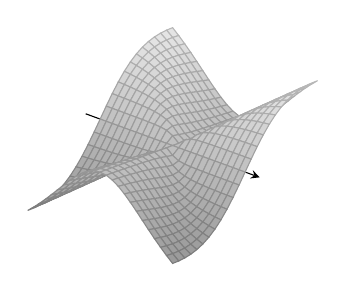
\begin{tikzpicture}[declare function={f(\x,\y)=-\x*(\y)^2/((\x)^2+(\y)^2);}]
  \begin{axis}[view/h=135,width=6cm,axis lines=center,domain=-2:2,domain y=-2:2,colormap={kgray}{gray(0.2cm)=(0.6);gray(1cm)=(0.9);},xtick={\empty},ytick={\empty},ztick={\empty},enlargelimits=true]
%\addplot3[contour gnuplot={output point meta=rawz,number=20,labels=false,},samples=41,z filter/.code=\def\pgfmathresult{-1.6},]{f(x,y)};
 \addplot3[surf,samples=25]{f(x,y)};
%\addplot3[contour gnuplot={draw color = red,levels={0.1,0.2,0.4}}]{f(x,y)};
\end{axis}
\end{tikzpicture}
\caption{}
\label{شکل_سوال_کثیرالمتغیر_ب}
\end{minipage}\hfill
\begin{minipage}{0.3\textwidth}
\centering
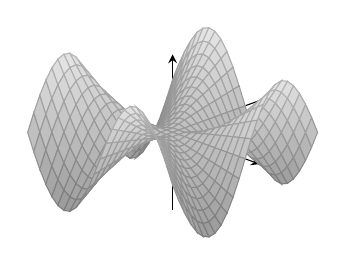
\begin{tikzpicture}[declare function={f(\x,\y)=\x*\y*((\x)^2-(\y)^2)/((\x)^2+(\y)^2);}]
  \begin{axis}[view/h=135,width=6cm,axis lines=center,domain=-2:2,domain y=-2:2,colormap={kgray}{gray(0.2cm)=(0.6);gray(1cm)=(0.9);},xtick={\empty},ytick={\empty},ztick={\empty},enlargelimits=true]
%\addplot3[contour gnuplot={output point meta=rawz,number=20,labels=false,},samples=41,z filter/.code=\def\pgfmathresult{-1.6},]{f(x,y)};
 \addplot3[surf,samples=25]{f(x,y)};
%\addplot3[contour gnuplot={draw color = red,levels={0.1,0.2,0.4}}]{f(x,y)};
\end{axis}
\end{tikzpicture}
\caption{}
\label{شکل_سوال_کثیرالمتغیر_ہ}
\end{minipage}\hfill
\begin{minipage}{0.3\textwidth}
\centering
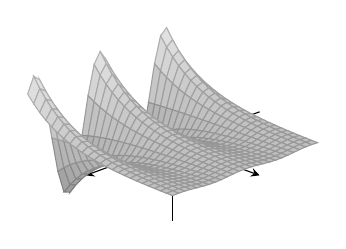
\begin{tikzpicture}[declare function={f(\x,\y)=e^(-\y)*cos(deg(\x));}]
  \begin{axis}[view/h=135,width=6cm,axis lines=center,domain=-7:7,domain y=-2:2,colormap={kgray}{gray(0.2cm)=(0.6);gray(1cm)=(0.9);},xtick={\empty},ytick={\empty},ztick={\empty},enlargelimits=true]
%\addplot3[contour gnuplot={output point meta=rawz,number=20,labels=false,},samples=41,z filter/.code=\def\pgfmathresult{-1.6},]{f(x,y)};
 \addplot3[surf,samples=25]{f(x,y)};
%\addplot3[contour gnuplot={draw color = red,levels={0.1,0.2,0.4}}]{f(x,y)};
\end{axis}
\end{tikzpicture}
\caption{}
\label{شکل_سوال_کثیرالمتغیر_د}
\end{minipage}
\begin{minipage}{0.3\textwidth}
\centering
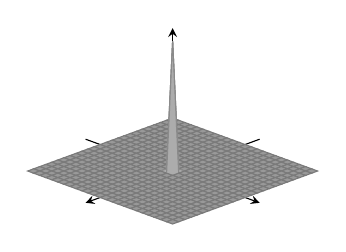
\begin{tikzpicture}[declare function={f(\x,\y)=1/(4*(\x)^2+(\y)^2);}]
  \begin{axis}[view/h=135,width=6cm,axis lines=center,domain=-2:2,domain y=-2:2,colormap={kgray}{gray(0.2cm)=(0.6);gray(1cm)=(0.9);},xtick={\empty},ytick={\empty},ztick={\empty},enlargelimits=true]
%\addplot3[contour gnuplot={output point meta=rawz,number=20,labels=false,},samples=41,z filter/.code=\def\pgfmathresult{-1.6},]{f(x,y)};
 \addplot3[surf,samples=25]{f(x,y)};
%\addplot3[contour gnuplot={draw color = red,levels={0.1,0.2,0.4}}]{f(x,y)};
\end{axis}
\end{tikzpicture}
\caption{}
\label{شکل_سوال_کثیرالمتغیر_ج}
\end{minipage}\hfill
\begin{minipage}{0.3\textwidth}
\centering
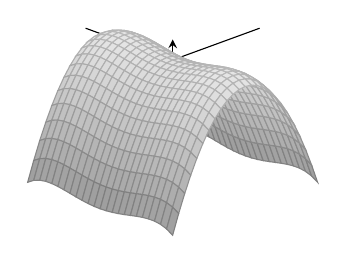
\begin{tikzpicture}[declare function={f(\x,\y)=(\y)^2-(\y)^4-(\x)^2;}]
  \begin{axis}[view/h=135,width=6cm,axis lines=center,domain=-2:2,domain y=-1:1,colormap={kgray}{gray(0.2cm)=(0.6);gray(1cm)=(0.9);},xtick={\empty},ytick={\empty},ztick={\empty},enlargelimits=true]
%\addplot3[contour gnuplot={output point meta=rawz,number=20,labels=false,},samples=41,z filter/.code=\def\pgfmathresult{-1.6},]{f(x,y)};
 \addplot3[surf,samples=25]{f(x,y)};
%\addplot3[contour gnuplot={draw color = red,levels={0.1,0.2,0.4}}]{f(x,y)};
\end{axis}
\end{tikzpicture}
\caption{}
\label{شکل_سوال_کثیرالمتغیر_و}
\end{minipage}\hfill
\begin{minipage}{0.3\textwidth}
\centering
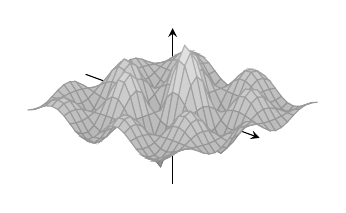
\begin{tikzpicture}[declare function={f(\x,\y)=cos(deg(\x))*sin(deg(\y))*e^(-1/4*sqrt((\x)^2+(\y)^2));}]
  \begin{axis}[view/h=135,width=6cm,axis lines=center,domain=-7:7,domain y=-7:7,colormap={kgray}{gray(0.2cm)=(0.6);gray(1cm)=(0.9);},xtick={\empty},ytick={\empty},ztick={\empty},enlargelimits=true]
%\addplot3[contour gnuplot={output point meta=rawz,number=20,labels=false,},samples=41,z filter/.code=\def\pgfmathresult{-1.6},]{f(x,y)};
 \addplot3[surf,samples=25]{f(x,y)};
%\addplot3[contour gnuplot={draw color = red,levels={0.1,0.2,0.4}}]{f(x,y)};
\end{axis}
\end{tikzpicture}
\caption{}
\label{شکل_سوال_کثیرالمتغیر_الف}
\end{minipage}
\end{figure}

%=====================
\موٹا{دو متغیرات کے تفاعل کی پہچان}\\
سوال \حوالہ{سوال_کثیرالمتغیر_ہم_قد_منحنیات_الف} تا سوال \حوالہ{سوال_کثیرالمتغیر_ہم_قد_منحنیات_ب} میں تفاعل کی قیمتوں کو دو طرح دکھائیں۔ (ا)  سطح \عددی{z=f(x,y)} کو ترسیم کرتے ہوئے اور (ب) تفاعل کے دائرہ کار میں منتخب ہم قد منحنیات ترسیم کرتے ہوئے۔ ہر ایک  ہم قد  منحنی  کی نشاندہی  تفاعل کی قیمت سے کریں۔  

\ابتدا{سوال}\شناخت{سوال_کثیرالمتغیر_ہم_قد_منحنیات_الف}
$f(x,y)=y^2$
\انتہا{سوال}  
   %======== 
  \ابتدا{جواب}
\wf{\unexpanded{
\begin{minipage}{0.45\textwidth}
\centering
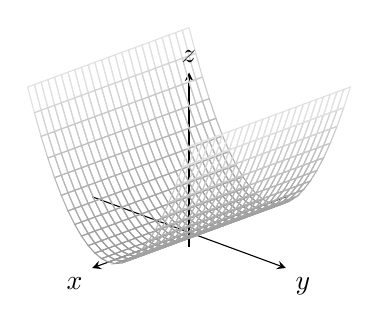
\begin{tikzpicture}[declare function={f(\x,\y)=(\y)^2;}]
  \begin{axis}[view/h=135,small,axis lines=center,domain=-1:1,domain y=-1:1,colormap={kgray}{gray(0.2cm)=(0.6);gray(1cm)=(0.9);},xtick={\empty},ytick={\empty},ztick={\empty},enlargelimits=true,xlabel={$x$},ylabel={$y$},zlabel={$z$},xlabel style={anchor=north east},ylabel style={anchor=north west},zlabel style={anchor=south}]
%\addplot3[, contour gnuplot={output point meta=rawz,number=4,labels=false,},samples=41,z filter/.code=\def\pgfmathresult{-1.6},]{f(x,y)};
 \addplot3[mesh,samples=25]{f(x,y)};
%\addplot3[, contour gnuplot={draw color = red,levels={0.1,0.2,0.4}}]{f(x,y)};
\end{axis}
\end{tikzpicture}
\end{minipage}\hfill
\begin{minipage}{0.45\textwidth}
\centering
\begin{tikzpicture}[declare function={f(\x,\y)=(\y)^2;}]
  \begin{axis}[view/h=135,small,axis lines=center,domain=-1:1,domain y=-1:1,colormap={kgray}{gray(0.2cm)=(0.6);gray(1cm)=(0.9);},xtick={\empty},ytick={\empty},ztick={\empty},enlargelimits=true,hide z axis,,xlabel={$x$},ylabel={$y$},zlabel={$z$},xlabel style={anchor=north east},ylabel style={anchor=north west},zlabel style={anchor=south},colormap={kdark}{gray(0.2cm)=(0.2);gray(1cm)=(0.2);}]
\addplot3[, contour gnuplot={output point meta=rawz,number=4,labels=true,},samples=41,z filter/.code=\def\pgfmathresult{0},]{f(x,y)};
 %\addplot3[mesh,samples=25]{f(x,y)};
%\addplot3[, contour gnuplot={draw color = red,levels={0.1,0.2,0.4}}]{f(x,y)};
\end{axis}
\end{tikzpicture}
\end{minipage}
}}
\انتہا{جواب}
%===================
\ابتدا{سوال}
$f(x,y)=4-y^2$
\انتہا{سوال}
%===================
\ابتدا{سوال}
$f(x,y)=x^2+y^2$
\انتہا{سوال}  
   %======== 
  \ابتدا{جواب}
\wf{\unexpanded{
\begin{minipage}{0.45\textwidth}
\centering
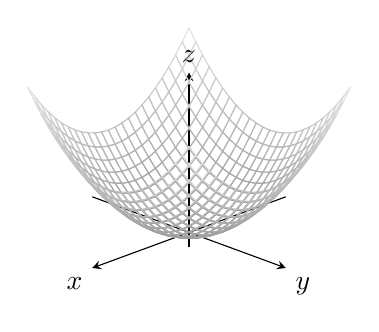
\begin{tikzpicture}[declare function={f(\x,\y)=(\x)^2+(\y)^2;}]
  \begin{axis}[view/h=135,small,axis lines=center,domain=-1:1,domain y=-1:1,colormap={kgray}{gray(0.2cm)=(0.6);gray(1cm)=(0.9);},xtick={\empty},ytick={\empty},ztick={\empty},enlargelimits=true,xlabel={$x$},ylabel={$y$},zlabel={$z$},xlabel style={anchor=north east},ylabel style={anchor=north west},zlabel style={anchor=south}]
%\addplot3[, contour gnuplot={output point meta=rawz,number=4,labels=false,},samples=41,z filter/.code=\def\pgfmathresult{-1.6},]{f(x,y)};
 \addplot3[mesh,samples=25]{f(x,y)};
%\addplot3[, contour gnuplot={draw color = red,levels={0.1,0.2,0.4}}]{f(x,y)};
\end{axis}
\end{tikzpicture}
\end{minipage}\hfill
\begin{minipage}{0.45\textwidth}
\centering
\begin{tikzpicture}[declare function={f(\x,\y)=(\x)^2+(\y)^2;}]
  \begin{axis}[view/h=135,small,axis lines=center,domain=-1:1,domain y=-1:1,colormap={kgray}{gray(0.2cm)=(0.6);gray(1cm)=(0.9);},xtick={\empty},ytick={\empty},ztick={\empty},enlargelimits=true,hide z axis,xlabel={$x$},ylabel={$y$},zlabel={$z$},xlabel style={anchor=north east},ylabel style={anchor=north west},zlabel style={anchor=south},colormap={kdark}{gray(0.2cm)=(0.2);gray(1cm)=(0.2);}]
\addplot3[, contour gnuplot={output point meta=rawz,number=4,labels=true,},samples=41,z filter/.code=\def\pgfmathresult{0},]{f(x,y)};
 %\addplot3[mesh,samples=25]{f(x,y)};
%\addplot3[, contour gnuplot={draw color = red,levels={0.1,0.2,0.4}}]{f(x,y)};
\end{axis}
\end{tikzpicture}
\end{minipage}
}}
\انتہا{جواب}
%===================
\ابتدا{سوال}
$f(x,y)=\sqrt{x^2+y^2}$
\انتہا{سوال}
%===================
\ابتدا{سوال}
$f(x,y)=-(x^2+y^2)$
\انتہا{سوال}  
   %======== 
  \ابتدا{جواب}
\wf{\unexpanded{
\begin{minipage}{0.45\textwidth}
\centering
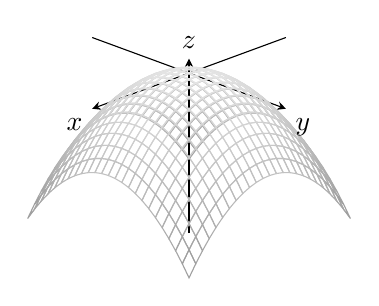
\begin{tikzpicture}[declare function={f(\x,\y)=-(\x)^2-(\y)^2;}]
  \begin{axis}[view/h=135,small,axis lines=center,domain=-1:1,domain y=-1:1,colormap={kgray}{gray(0.2cm)=(0.6);gray(1cm)=(0.9);},xtick={\empty},ytick={\empty},ztick={\empty},enlargelimits=true,xlabel={$x$},ylabel={$y$},zlabel={$z$},xlabel style={anchor=north east},ylabel style={anchor=north west},zlabel style={anchor=south}]
%\addplot3[, contour gnuplot={output point meta=rawz,number=4,labels=false,},samples=41,z filter/.code=\def\pgfmathresult{-1.6},]{f(x,y)};
 \addplot3[mesh,samples=25]{f(x,y)};
%\addplot3[, contour gnuplot={draw color = red,levels={0.1,0.2,0.4}}]{f(x,y)};
\end{axis}
\end{tikzpicture}
\end{minipage}\hfill
\begin{minipage}{0.45\textwidth}
\centering
\begin{tikzpicture}[declare function={f(\x,\y)=-(\x)^2-(\y)^2;}]
  \begin{axis}[view/h=135,width=6cm,axis lines=center,domain=-1:1,domain y=-1:1,colormap={kgray}{gray(0.2cm)=(0.6);gray(1cm)=(0.9);},xtick={\empty},ytick={\empty},ztick={\empty},enlargelimits=true,hide z axis,xlabel={$x$},ylabel={$y$},zlabel={$z$},xlabel style={anchor=north east},ylabel style={anchor=north west},zlabel style={anchor=south},colormap={kdark}{gray(0.2cm)=(0.2);gray(1cm)=(0.2);}]
\addplot3[, contour gnuplot={output point meta=rawz,number=4,labels=true,},samples=41,z filter/.code=\def\pgfmathresult{0},]{f(x,y)};
 %\addplot3[mesh,samples=25]{f(x,y)};
%\addplot3[, contour gnuplot={draw color = red,levels={0.1,0.2,0.4}}]{f(x,y)};
\end{axis}
\end{tikzpicture}
\end{minipage}
}}
\انتہا{جواب}
%===================
\ابتدا{سوال}
$f(x,y)=4-x^2-y^2$
\انتہا{سوال}
%===================
\ابتدا{سوال}
$f(x,y)=4x^2+y^2$
\انتہا{سوال}  
   %======== 
  \ابتدا{جواب}
\wf{\unexpanded{
\begin{minipage}{0.45\textwidth}
\centering
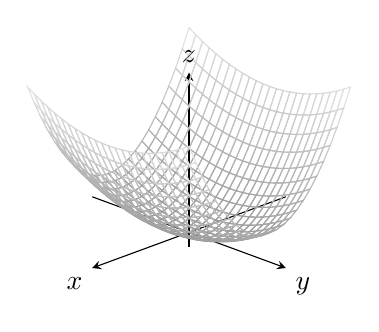
\begin{tikzpicture}[declare function={f(\x,\y)=4*(\x)^2+(\y)^2;}]
  \begin{axis}[view/h=135,small,axis lines=center,domain=-1:1,domain y=-1:1,colormap={kgray}{gray(0.2cm)=(0.6);gray(1cm)=(0.9);},xtick={\empty},ytick={\empty},ztick={\empty},enlargelimits=true,xlabel={$x$},ylabel={$y$},zlabel={$z$},xlabel style={anchor=north east},ylabel style={anchor=north west},zlabel style={anchor=south}]
%\addplot3[, contour gnuplot={output point meta=rawz,number=4,labels=false,},samples=41,z filter/.code=\def\pgfmathresult{-1.6},]{f(x,y)};
 \addplot3[mesh,samples=25]{f(x,y)};
%\addplot3[, contour gnuplot={draw color = red,levels={0.1,0.2,0.4}}]{f(x,y)};
\end{axis}
\end{tikzpicture}
\end{minipage}\hfill
\begin{minipage}{0.45\textwidth}
\centering
\begin{tikzpicture}[declare function={f(\x,\y)=4*(\x)^2+(\y)^2;}]
  \begin{axis}[view/h=135,small,axis lines=center,domain=-1:1,domain y=-1:1,colormap={kgray}{gray(0.2cm)=(0.6);gray(1cm)=(0.9);},xtick={\empty},ytick={\empty},ztick={\empty},enlargelimits=true,hide z axis,xlabel={$x$},ylabel={$y$},zlabel={$z$},xlabel style={anchor=north east},ylabel style={anchor=north west},zlabel style={anchor=south},colormap={kdark}{gray(0.2cm)=(0.2);gray(1cm)=(0.2);}]
\addplot3[, contour gnuplot={output point meta=rawz,number=4,labels=true,},samples=41,z filter/.code=\def\pgfmathresult{0},]{f(x,y)};
 %\addplot3[mesh,samples=25]{f(x,y)};
%\addplot3[, contour gnuplot={draw color = red,levels={0.1,0.2,0.4}}]{f(x,y)};
\end{axis}
\end{tikzpicture}
\end{minipage}
}}
\انتہا{جواب}
%===================
\ابتدا{سوال}
$f(x,y)=4x^2+y^2+1$
\انتہا{سوال}
%===================
\ابتدا{سوال}
$f(x,y)=1-\abs{y}$
\انتہا{سوال}  
   %======== 
  \ابتدا{جواب}
\wf{\unexpanded{
\begin{minipage}{0.45\textwidth}
\centering
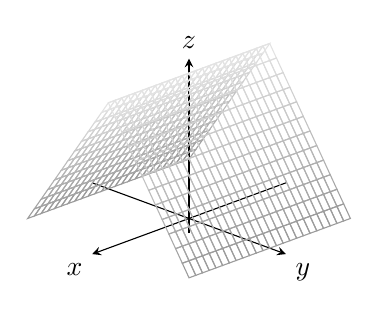
\begin{tikzpicture}[declare function={f(\x,\y)=1-abs(\y);}]
  \begin{axis}[view/h=135,small,axis lines=center,domain=-1:1,domain y=-1:1,colormap={kgray}{gray(0.2cm)=(0.6);gray(1cm)=(0.9);},xtick={\empty},ytick={\empty},ztick={\empty},enlargelimits=true,xlabel={$x$},ylabel={$y$},zlabel={$z$},xlabel style={anchor=north east},ylabel style={anchor=north west},zlabel style={anchor=south}]
%\addplot3[, contour gnuplot={output point meta=rawz,number=4,labels=false,},samples=41,z filter/.code=\def\pgfmathresult{-1.6},]{f(x,y)};
 \addplot3[mesh,samples=25]{f(x,y)};
%\addplot3[, contour gnuplot={draw color = red,levels={0.1,0.2,0.4}}]{f(x,y)};
\end{axis}
\end{tikzpicture}
\end{minipage}\hfill
\begin{minipage}{0.45\textwidth}
\centering
\begin{tikzpicture}[declare function={f(\x,\y)=1-abs(\y);}]
  \begin{axis}[view/h=135,small,axis lines=center,domain=-1:1,domain y=-1:1,colormap={kgray}{gray(0.2cm)=(0.6);gray(1cm)=(0.9);},xtick={\empty},ytick={\empty},ztick={\empty},enlargelimits=true,hide z axis,xlabel={$x$},ylabel={$y$},zlabel={$z$},xlabel style={anchor=north east},ylabel style={anchor=north west},zlabel style={anchor=south},colormap={kdark}{gray(0.2cm)=(0.2);gray(1cm)=(0.2);}]
\addplot3[, contour gnuplot={output point meta=rawz,number=4,labels=true,},samples=41,z filter/.code=\def\pgfmathresult{0},]{f(x,y)};
 %\addplot3[mesh,samples=25]{f(x,y)};
%\addplot3[, contour gnuplot={draw color = red,levels={0.1,0.2,0.4}}]{f(x,y)};
\end{axis}
\end{tikzpicture}
\end{minipage}
}}
\انتہا{جواب}
%===================
\ابتدا{سوال}\شناخت{سوال_کثیرالمتغیر_ہم_قد_منحنیات_ب}
$f(x,y)=1-\abs{x}-\abs{y}$
\انتہا{سوال}
%===================

\موٹا{ہم قد سطحیں}\\
سوال \حوالہ{سوال_کثیر_المتغیر_ہم_قد_سطح_الف} تا سوال \حوالہ{سوال_کثیر_المتغیر_ہم_قد_سطح_ب} میں تفاعل کا  ایک علامتی  ہم قد سطح  کا خاکہ بنائیں۔

\ابتدا{سوال}\شناخت{سوال_کثیر_المتغیر_ہم_قد_سطح_الف}
$f(x,y,z)=x^2+y^2+z^2$
\انتہا{سوال}  
   %======== 
  \ابتدا{جواب}
\wf{\unexpanded{
\begin{center}
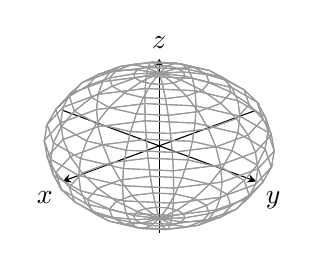
\begin{tikzpicture}[declare function={fx(\x,\y)=sin(\x)*cos(\y);fy(\x,\y)=sin(\x)*sin(\y);fz(\x,\y)=cos(\x);}]
  \begin{axis}[view/h=135,small,axis lines=center,domain=0:180,domain y=0:360,colormap={kgray}{gray(0.2cm)=(0.6);gray(1cm)=(0.6);},xtick={\empty},ytick={\empty},ztick={\empty},enlargelimits=true,xlabel={$x$},ylabel={$y$},zlabel={$z$},xlabel style={anchor=north east},ylabel style={anchor=north west},zlabel style={anchor=south}]
%\addplot3[, contour gnuplot={output point meta=rawz,number=4,labels=false,},samples=41,z filter/.code=\def\pgfmathresult{0},]{f(x,y)};
 \addplot3[mesh,samples=15]({fx(x,y)},{fy(x,y)},{fz(x,y)});
%\addplot3[, contour gnuplot={draw color = red,levels={0.1,0.2,0.4}}]({fx(x,y)},{fy(x,y)},{fz(x,y)});
\end{axis}
\end{tikzpicture}
\end{center}
$f(x,y,z)=x^2+y^2+z^2=1$
}}
\انتہا{جواب}
%==================
\ابتدا{سوال}
$f(x,y,z)=\ln(x^2+y^2+z^2)$
\انتہا{سوال}
%================
\ابتدا{سوال}
$f(x,y,z)=x+z$
\انتہا{سوال}  
   %======== 
  \ابتدا{جواب}
\wf{\unexpanded{
\begin{center}
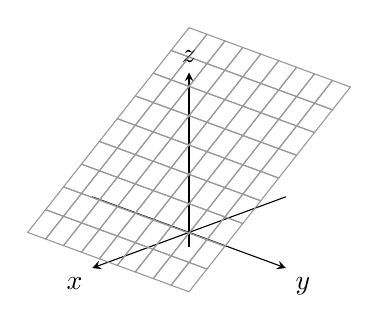
\begin{tikzpicture}[declare function={f(\x,\y)=1-\x;}]
  \begin{axis}[view/h=135,small,axis lines=center,domain=-1:1,domain y=-1:1,colormap={kgray}{gray(0.2cm)=(0.6);gray(1cm)=(0.6);},xtick={\empty},ytick={\empty},ztick={\empty},enlargelimits=true,xlabel={$x$},ylabel={$y$},zlabel={$z$},xlabel style={anchor=north east},ylabel style={anchor=north west},zlabel style={anchor=south}]
%\addplot3[, contour gnuplot={output point meta=rawz,number=4,labels=false,},samples=41,z filter/.code=\def\pgfmathresult{0},]{f(x,y)};
 \addplot3[mesh,samples=10]{f(x,y)};
%\addplot3[, contour gnuplot={draw color = red,levels={0.1,0.2,0.4}}]{f(x,y)};
\end{axis}
\end{tikzpicture}
\end{center}
$f(x,y,z)=x+z=1$
}}
\انتہا{جواب}
%================
\ابتدا{سوال}
$f(x,y,z)=z$
\انتہا{سوال}
%================
\ابتدا{سوال}
$f(x,y,z)=x^2+y^2$
\انتہا{سوال}  
   %======== 
  \ابتدا{جواب}
\wf{\unexpanded{
\begin{center}
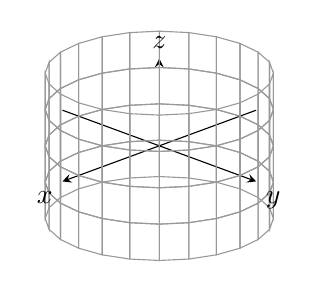
\begin{tikzpicture}[declare function={fx(\x,\y)=cos(\x);fy(\x,\y)=sin(\x);fz(\x,\y)=\y;}]
  \begin{axis}[view/h=135,small,axis lines=center,domain=0:360,domain y=-1:1,colormap={kgray}{gray(0.2cm)=(0.6);gray(1cm)=(0.6);},xtick={\empty},ytick={\empty},ztick={\empty},enlargelimits=true,xlabel={$x$},ylabel={$y$},zlabel={$z$},xlabel style={anchor=north east},ylabel style={anchor=north west},zlabel style={anchor=south}]
%\addplot3[, contour gnuplot={output point meta=rawz,number=4,labels=false,},samples=41,z filter/.code=\def\pgfmathresult{0},]{f(x,y)};
 \addplot3[smooth,mesh,samples=25,samples y=5]({fx(x,y)},{fy(x,y)},{fz(x,y)});
%\addplot3[, contour gnuplot={draw color = red,levels={0.1,0.2,0.4}}]({fx(x,y)},{fy(x,y)},{fz(x,y)});
\end{axis}
\end{tikzpicture}
\end{center}
$f(x,y,z)=x^2+y^2=1$
}}
\انتہا{جواب}
%================
\ابتدا{سوال}
$f(x,y,z)=y^2+z^2$
\انتہا{سوال}
%================
\ابتدا{سوال}
$f(x,y,z)=z-x^2-y^2$
\انتہا{سوال}  
   %======== 
  \ابتدا{جواب}
\wf{\unexpanded{
\begin{center}
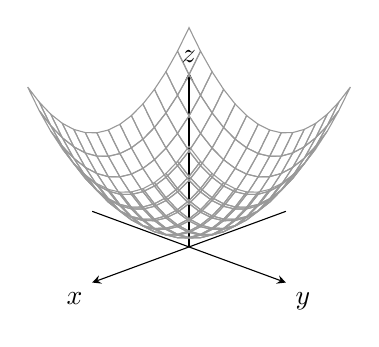
\begin{tikzpicture}[declare function={f(\x,\y)=1+(\x)^2+(\y)^2;}]
  \begin{axis}[view/h=135,small,axis lines=center,domain=-1:1,domain y=-1:1,colormap={kgray}{gray(0.2cm)=(0.6);gray(1cm)=(0.6);},xtick={\empty},ytick={\empty},ztick={\empty},enlargelimits=true,xlabel={$x$},ylabel={$y$},zlabel={$z$},xlabel style={anchor=north east},ylabel style={anchor=north west},zlabel style={anchor=south}]
%\addplot3[, contour gnuplot={output point meta=rawz,number=4,labels=false,},samples=41,z filter/.code=\def\pgfmathresult{0},]{f(x,y)};
 \addplot3[mesh,samples=15]{f(x,y)};
%\addplot3[, contour gnuplot={draw color = red,levels={0.1,0.2,0.4}}]{f(x,y)};
\end{axis}
\end{tikzpicture}
\end{center}
$f(x,y,z)=z-x^2-y^2=1$\\
یعنی
$z=x^2+y^2+1$
}}
\انتہا{جواب}
%================
\ابتدا{سوال}\شناخت{سوال_کثیر_المتغیر_ہم_قد_سطح_ب}
$f(x,y,z)=\tfrac{x^2}{25}+\tfrac{y^2}{16}+\tfrac{z^2}{9}$
\انتہا{سوال}
%================
\موٹا{ہم قد منحنی کی  تلاش}\\
سوال \حوالہ{سوال_کثیر_المتغیر_ہم_قد_منحنی_تلاش_الف} تا سوال \حوالہ{سوال_کثیر_المتغیر_ہم_قد_منحنی_تلاش_ب} میں  تفاعل \عددی{f(x,y)} کی اس  ہم قد منحنی کی مساوات تلاش کریں جو  دیے گئے نقطہ سے گزرتی  ہو۔

\ابتدا{سوال}\شناخت{سوال_کثیر_المتغیر_ہم_قد_منحنی_تلاش_الف}
$f(x,y)=16-x^2-y^2,\quad (2\sqrt{2},\sqrt{2})$
\انتہا{سوال}  
   %======== 
  \ابتدا{جواب}
\wf{\unexpanded{
$x^2+y^2=10$
}}
\انتہا{جواب}
%================
\ابتدا{سوال}
$f(x,y)=\sqrt{x^2-1},\quad (1,0)$
\انتہا{سوال}
%================
\ابتدا{سوال}
$f(x,y)=\int\limits_x^y\frac{\dif t}{1+t^2},\quad (-\sqrt{2},\sqrt{2})$
\انتہا{سوال}  
   %======== 
  \ابتدا{جواب}
\wf{\unexpanded{
$\tan^{-1}y-\tan^{-1}x=2\tan^{-1}\sqrt{2}$
}}
\انتہا{جواب}
%================
\ابتدا{سوال}\شناخت{سوال_کثیر_المتغیر_ہم_قد_منحنی_تلاش_ب}
$f(x,y)=\sum\limits_{n=0}^{\infty}\big(\frac{x}{y}\big)^n,\quad (1,2)$
\انتہا{سوال}
%================
\موٹا{ہم قد سطح کی تلاش}\\
سوال \حوالہ{سوال_کثیر_المتغیر_ہم_قد_سطح_تلاش_الف} تا سوال \حوالہ{سوال_کثیر_المتغیر_ہم_قد_سطح_تلاش_ب} میں دیے گئے نقطہ سے گزرتی ہم قد سطح کی مساوات تلاش کریں۔

\ابتدا{سوال}\شناخت{سوال_کثیر_المتغیر_ہم_قد_سطح_تلاش_الف}
$f(x,y,z)=\sqrt{x-y}-\ln z,\quad (3,-1,1)$
\انتہا{سوال}  
   %======== 
  \ابتدا{جواب}
\wf{\unexpanded{
$\sqrt{x-y}-\ln z=2$
}}
\انتہا{جواب}
%=================
\ابتدا{سوال}
$f(x,y,z)=\ln(x^2+y+z^2),\quad (-1,2,1)$
\انتہا{سوال}
%==================
\ابتدا{سوال}
$g(x,y,z)=\sum\limits_{n=0}^{\infty}\frac{(x+y)^n}{n!z^n},\quad (\ln 2,\ln 4,3)$
\انتہا{سوال}  
   %======== 
  \ابتدا{جواب}
\wf{\unexpanded{
$\tfrac{x+y}{z}=\ln 2$
}}
\انتہا{جواب}
%==================
\ابتدا{سوال}\شناخت{سوال_کثیر_المتغیر_ہم_قد_سطح_تلاش_ب}
$g(x,y,z)=\int\limits_x^y\frac{\dif \theta}{\sqrt{1-\theta^2}}+\int\limits_{\sqrt{2}}^{z}\frac{\dif t}{t\sqrt{t^2-1}},\quad (0,\tfrac{1}{2},2)$
\انتہا{سوال}
%==================

\موٹا{نظریہ اور مثالیں}\\
\ابتدا{سوال}\ترچھا{فضا میں ایک لکیر پر تفاعل کی زیادہ سے زیادہ قیمت۔}\\
کیا لکیر \عددی{x=20-t,\,y=t,\,z=20} پر تفاعل \عددی{f(x,y,z)=xyz} کی  زیادہ سے زیادہ قیمت پائی جاتی ہے؟ اگر  ہو، تب اس کی قیمت کتنی ہو گی؟ اپنے جواب کی وجہ پیش کریں۔ (اشارہ:اس لکیر پر \عددی{w=(f,y,z)} متغیر \عددی{t} کا قابل تفرق تفاعل ہے۔)
\انتہا{سوال}  
   %======== 
  \ابتدا{جواب}
\wf{\unexpanded{
جی ہاں، \عددی{2000}
}}
\انتہا{جواب}
%==============
\ابتدا{سوال}\ترچھا{فضا میں ایک لکیر پر تفاعل کی کم سے کم  قیمت۔}\\
کیا لکیر \عددی{x=t-1,\,y=t-2,\,z=t+7} پر تفاعل \عددی{f(x,y,z)=xy-z} کی کم سے کم  قیمت پائی جاتی ہے؟ اگر  ہو، تب اس کی قیمت کتنی ہو گی؟ اپنے جواب کی وجہ پیش کریں۔ (اشارہ:اس لکیر پر \عددی{w=(f,y,z)} متغیر \عددی{t} کا قابل تفرق تفاعل ہے۔)
\انتہا{سوال}
%=================
\ابتدا{سوال}\ترچھا{جہاز کا صوتی دھماکا}\\
ایک جہاز کے نیچے زمین پر اس خطہ کی چوڑائی \عددی{w}  جہاں  جہاز کا   صوتی دھماکا   انسان  برائے راست (جو   فضا میں ہوا کی مختلف  سطحوں سے منعکس نہ ہو)  سن سکتا ہو  ، درج ذیل کا  تفاعل ہو گا۔
\begin{itemize}
\item
\عددی{T} زمین پر ہوا کی  درجہ حرارت (کیلون) 
\item
\عددی{h} جہاز کی بلندی (کلو میٹر)
\item
\عددی{d}  درجہ حرارت کی انتصابی  شرح تبدیلی (کیلون فی کلومیٹر)
\end{itemize}
اس چوڑائی کا  کلیہ درج ذیل ہے۔
\begin{align*}
w=4\sqrt{\tfrac{Th}{d}}
\end{align*}
یہ جہاز \عددی{\SI{16.8}{\kilo\meter}} کی بلندی پر پرواز کرتا ہوا  بحیرہ عرب  سے کراچی  شہر    پہنچ رہا ہے۔ اگر سطحی درجہ حرارت \عددی{\SI{290}{\kelvin}} اور انتصابی شرح حرارت \عددی{\SI{5}{\kelvin\per\kilo\meter}} ہو تب   جہاز ساحل سے کتنا دور ہو گا جب اس کا صوتی دھماکا سنائی دے۔
\انتہا{سوال}  
   %======== 
  \ابتدا{جواب}
\wf{\unexpanded{
$\SI{63}{\kilo\meter}$
}}
\انتہا{جواب}
%================
\ابتدا{سوال}
جیسا کہ آپ جانتے ہیں، واحد حقیقی متغیر کے حقیقی قیمت تفاعل کی ترسیم دو محددی فضا کا سلسلہ ہو تا ہے۔ دو غیر تابع حقیقی متغیرات کے حقیقی قیمت تفاعل  کی ترسیم تین محددی فضا کا سلسلہ ہوتا ہے۔    تین غیر تابع حقیقی متغیرات کے حقیقی قیمت تفاعل  کی ترسیم چار  محددی فضا کا سلسلہ ہوتا ہے۔   آپ چار غیر تابع متغیرات کے تفاعل \عددی{f(x_1,x_2,x_3,x_4)}  کی ترسیم کے بارے میں کیا کہیں گے؟ ۔   آپ \عددی{n}  غیر تابع متغیرات کے تفاعل \عددی{f(x_1,x_2,x_3,\cdots,x_n)}  کی ترسیم کے بارے میں کیا کہیں گے؟
\انتہا{سوال}
%==========
\موٹا{کمپیوٹر کا استعمال۔صریح سطح}\\
کمپیوٹر استعمال کرتے ہوئے سوال \حوالہ{سوال_کثیرالمتغیر_صریح_سطح_الف} تا سوال \حوالہ{سوال_کثیرالمتغیر_صریح_سطح_ب} میں درج ذیل اقدام کریں۔
\begin{enumerate}[a.]
\item
دیے گئے مستطیل پر سطح ترسیم کریں۔
\item
اس مستطیل میں کئی ہم قد منحنیات ترسیم کریں۔
\item
دیے گئے نقطہ سے گزرتی  ہوئی   \عددی{f} کی   ہم قد منحنی ترسیم کریں۔ 
\end{enumerate}

\ابتدا{سوال}\شناخت{سوال_کثیرالمتغیر_صریح_سطح_الف}
$f(x,y)=x\sin\tfrac{y}{2}+y\sin 2x,\quad 0\le x\le 5\pi,\quad 0\le y\le 5\pi$
\انتہا{سوال}
%=================
\ابتدا{سوال}
$f(x,y)=(\sin x)(\cos x)e^{\sqrt{x^2+y^2}/8},\quad 0\le x\le 5\pi,\quad 0\le y\le 5\pi$
\انتہا{سوال}
%==================
\ابتدا{سوال}
$f(x,y)=\sin(x+2\cos y),\quad -2\pi\le x\le 2\pi,\quad -2\pi\le y\le 2\pi$
\انتہا{سوال}
%==================
\ابتدا{سوال}\شناخت{سوال_کثیرالمتغیر_صریح_سطح_ب}
$f(x,y)=e^{(x^{0.1}-y)}\sin (x^2+y^2),\quad 0\le x\le 2\pi,\quad -2\pi\le y\le \pi$
\انتہا{سوال}
%==================
\موٹا{کمپیوٹر کا استعمال۔خفی  سطح}\\
سوال \حوالہ{سوال_کثیرالمتغیر_ہم_قد_سطحیں_ترسیم_الف} تا سوال \حوالہ{سوال_کثیرالمتغیر_ہم_قد_سطحیں_ترسیم_ب} میں کمپیوٹر استعمال کرتے ہوئے ہم قد سطحیں  ترسیم کریں۔

\ابتدا{سوال}\شناخت{سوال_کثیرالمتغیر_ہم_قد_سطحیں_ترسیم_الف}
$4\ln(x^2+y^2+z^2)=1$
\انتہا{سوال}
%================
\ابتدا{سوال}
$x^2+z^2=1$
\انتہا{سوال}
%=====================
\ابتدا{سوال}
$x+y^2-3z^2=1$
\انتہا{سوال}
%=====================
\ابتدا{سوال}\شناخت{سوال_کثیرالمتغیر_ہم_قد_سطحیں_ترسیم_ب}
$\sin\big(\frac{x}{2}\big)-(\cos y)\sqrt{x^2+z^2}=2$
\انتہا{سوال}
%=====================
\موٹا{کمپیوٹر کا استعمال۔مقدار معلوم   سطح}\\
جیسا آپ کسی مقدار معلوم وقفہ \عددی{I} پر  مستوی میں منحنیات کو مقدار معلوم مساوات \عددی{x=f(t),\,y=g(t)} کی    روپ میں لکھتے ہیں، آپ بعض اوقات کسی مقدار معلوم مستطیل \عددی{a\le u\le b,\, c\le v\le d}وقفہ  پر  فضا میں سطحوں کو    مقدار معلوم تین مساوات \عددی{x=f(u,v),\,y=g(u,v),\,z=h(u,v)}  کی روپ میں لکھ سکتے ہیں۔کمپیوٹر اس قسم کی مقدار معلوم مساواتوں سے سطح  ترسیم کر سکتا ہے۔سوال \حوالہ{سوال_کثیرالمتغیر_مقدار_معلوم_الف} تا سوال \حوالہ{سوال_کثیرالمتغیر_مقدار_معلوم_ب} میں کمپیوٹر کی مدد سے سطحیں ترسیم کریں۔ساتھ ہی \عددی{xy} مستوی میں چند ہم قد منحنیات ترسیم کریں۔

\ابتدا{سوال}\شناخت{سوال_کثیرالمتغیر_مقدار_معلوم_الف}
$x=u\cos v,\quad y=u\sin v,\quad z=u,\quad 0\le u\le 2,\quad 0\le v\le 2\pi$
\انتہا{سوال}
%===================
\ابتدا{سوال}
$x=u\cos v,\quad y=u\sin v,\quad z=v,\quad 0\le u\le 2,\quad 0\le v\le 2\pi$
\انتہا{سوال}
%===================
\ابتدا{سوال}
$x=(2+\cos u)\cos v,\,y=(2+\cos u)\sin v,\, z=\sin u,$\\
$ 0\le u\le 2\pi,\, 0\le v\le 2\pi$
\انتہا{سوال}
%===================
\ابتدا{سوال}\شناخت{سوال_کثیرالمتغیر_مقدار_معلوم_ب}
$x=2\cos u\cos v,\quad y=2\cos u\sin v,\quad z=2\sin u$\\
$0\le u\le 2\pi,\quad 0\le v\le \pi$
\انتہا{سوال}
%======================
\انتہا{سوالات}




\حصہ{حد اور استمرار}
اس حصہ میں کثیر المتغیر تفاعل کی حد اور استمرار پر غور کیا جائے گا۔

\جزوحصہء{حد}
اگر نقطہ \عددی{(x_0,y_0)} کے قریب   تمام نقاط \عددی{(x,y) } کے لئے تفاعل \عددی{f(x,y)}  کی قیمتیں کسی  مقررہ حقیقی عدد \عددی{L} کے  بہت  زیادہ  قریب ہوں تب ہم کہتے ہیں کہ جیسے جیسے \عددی{(x,y)} نقطہ \عددی{(x_0,y_0)} تک  پہنچنے کی کوشش کرتا ہے، تفاعل \عددی{f} کی قیمت \عددی{L} تک پہنچنے کی کوشش کرتی ہے۔ یہ تعریف، واحد متغیر کے تفاعل کی حد کی تعریف کی مانند ہے۔البتہ، دھیان رہے کہ اگر \عددی{(x_0,y_0)} تفاعل \عددی{f}  کے دائرہ کار  کی اندرون میں پایا جاتا ہو تب \عددی{(x,y)} نقطہ \عددی{(x_0,y_0)} تک کسی بھی رخ سے پہنچنے کی کوشش کر سکتا ہے۔جیسا آپ نیچے  دی گئی   مثالوں میں سے چند  میں دیکھیں گے،  قریب پہنچنے کا رخ بعض اوقات مسئلہ کھڑا کر سکتا ہے۔

\ابتدا{تعریف}
اگر ہر عدد \عددی{\epsilon>0} کے لئے ایسا مطابقتی عدد \عددی{\delta>0} پایا جاتا ہو کہ \عددی{f} کے دائرہ کار میں تمام \عددی{(x,y)} کے لئے 
\begin{align}\label{مساوات_کثیرالمتغیر_تعریف_حد_الف}
0<\sqrt{(x-x_0)^2+(y-y_0)^2}<\delta\implies \abs{f(x,y)-L}<\epsilon
\end{align}
ہو ، تب ہم کہتے ہیں کہ \عددی{(x_0,y_0)} تک  \عددی{(x,y)}    پہنچنے سے \عددی{f(x,y)} کی قیمت \اصطلاح{حد}\فرہنگ{حد}\حاشیہب{limit}\فرہنگ{limit} \عددی{L} تک پہنچتی ہے جس کو ہم درج ذیل لکھتے ہیں۔
\begin{align*}
\lim_{(x,y)\to(x_0,y_0)}f(x,y)=L
\end{align*}
\انتہا{تعریف}
%====================

حد کی تعریف میں \عددی{\delta \sigma} کی شرط  اس کی  معادل ہے  کہ، کسی بھی \عددی{\epsilon>0} کے لئے ایسا مطابقتی \عددی{\delta>0} پایا جاتا ہو کہ تمام \عددی{x} کے لئے درج ذیل ہو۔
\begin{align}\label{مساوات_کثیرالمتغیر_تعریف_حد_ب}
0<\abs{x-x_0}<\delta\quad \text{اور}\quad 0<\abs{y-y_0}<\delta\implies \abs{f(x,y)-L}<\epsilon
\end{align}
یوں حد کی قیمت  تلاش کرتے   ہوئے ہم مستوی میں فاصلوں کی صورت یا محدد میں فرق کی صورت میں سوچ سکتے ہیں۔

حد کی تعریف، تفاعل \عددی{f} کے دائرہ کار کی اندرون  کے ساتھ   سرحدی نقاط \عددی{(x_0,y_0)} کے لئے بھی   کارآمد  ہے۔  بس اتنا ضروری ہے کہ نقطہ \عددی{(x,y)} ہر وقت دائرہ کار کے اندر رہے۔

واحد متغیر کے تفاعل کی طرح  درج ذیل دکھائے جا  سکتے ہیں۔
\begin{gather}
\begin{aligned}\label{مساوات_کثیر_المتغیر_قواعد_حد}
\lim_{(x,y)\to(x_0,y_0)}x&=x_0\\
\lim_{(x,y)\to(x_0,y_0)}y&=y_0\\
\lim_{(x,y)\to(x_0,y_0)}k&=k\quad \text{\RL{\عددی{k} کوئی بھی عدد ہو سکتا ہے}}
\end{aligned}
\end{gather}
یہ بھی دکھایا جا سکتا ہے کہ دو تفاعل کے مجموعہ کا حد، ان تفاعل کے انفرادی حد   (اگر دونوں موجود ہوں)کا مجموعہ ہو گا۔اسی طرح   کے نتائج   فرق، حاصل ضرب، حاصل تقسیم، مستقل مضرب اور طاقت کے لئے بھی دکھائے جا سکتے ہیں۔

\ابتدا{مسئلہ}\شناخت{مسئلہ_کثیر_المتغیر_قواعد_حد}\موٹا{دو متغیرات کے تفاعل کی حد کے خواص}\\
اگر 
\begin{align*}
\lim_{(x,y)\to(x_0,y_0)}f(x,y)=L\quad \text{اور}\quad \lim_{(x,y)\to(x_0,y_0)}g(x,y)=M
\end{align*}
ہوں تب درج ذیل قواعد کارآمد  ہوں گے۔
\begin{description}
\item{قاعدہ مجموعہ:}
$\lim[f(x,y)+g(x,y)]=L+M$
\item{قاعدہ فرق:}
$\lim[f(x,y)-g(x,y)]=L-M$
\item{قاعدہ مستقل مضرب:}
$\lim kf(x,y)=kL$
جہاں \عددی{k} کوئی مستقل ہے۔
\item{قاعدہ حاصل تقسیم:}
$\lim\frac{f(x,y)}{g(x,y)}=\frac{L}{M}$
اگر  \عددی{M\ne 0} ہو۔
\item{قاعدہ طاقت:}
$\lim[f(x,y)]^{m/n}=L^{m/n}$
اگر  \عددی{m} اور \عددی{n}ا عداد صحیح   اور \عددی{L^{m/n}} ایک حقیقی عدد ہو۔
\end{description}
تمام حد \عددی{(x,y)\to (x_0,y_0)} کی صورت میں حاصل کیے جائیں گے اور \عددی{L}، \عددی{M} کا حقیقی اعداد ہونا لازمی ہے۔
\انتہا{مسئلہ}
%==========

 مساوات \حوالہ{مساوات_کثیر_المتغیر_قواعد_حد} پر   مسئلہ \حوالہ{مسئلہ_کثیر_المتغیر_قواعد_حد} کے اطلاق سے ہمیں معلوم ہوتا ہے کہ  \عددی{(x,y)\to(x_0,y_0)} کرتے ہوئے  کثیر رکنی اور ناطق تفاعل کی حد     ہم \عددی{(x_0,y_0)} پر  تفاعل کی قیمت   سے حاصل کرتے  ہیں۔ بس اتنا ضروری  ہے کہ  نقطہ \عددی{(x_0,y_0)} پر تفاعل  معین ہو۔

\ابتدا{مثال}
\begin{align*}
\lim_{(x,y)\to(0,1)}\frac{x-xy+3}{x^2y+5xy-y^3}&=\frac{0-(0)(1)+3}{(0)^2(1)+5(0)(1)-(1)^3}=-3\\
\lim_{(x,y)\to(3,-4)}\sqrt{x^2+y^2}&=\sqrt{(3)^2+(-4)^2}=\sqrt{25}=5
\end{align*}
\انتہا{مثال}
%=================
\ابتدا{مثال}
درج ذیل حاصل کریں۔
\begin{align*}
\lim_{(x,y)\to(0,0)}\frac{x^2-xy}{\sqrt{x}-\sqrt{y}}
\end{align*}
حل:\quad
چونکہ \عددی{(x,y)\to(0,0)} پر نسب نما   \عددی{ 0} کو پہنچتا ہے لہٰذا  ہم  قاعدہ حاصل تقسیم (مسئلہ \حوالہ{مسئلہ_کثیر_المتغیر_قواعد_حد})  استعمال نہیں کر سکتے ہیں۔ البتہ نسب نما اور شمار کنندہ کو \عددی{\sqrt{x}+\sqrt{y}} سے ضرب  دے کر ایسا معادل حاصل تقسیم حاصل ہوتا ہے جس کا حد ہم تلاش کر سکتے ہیں:
\begin{align*}
\lim_{(x,y)\to(0,0)}\frac{x^2-xy}{\sqrt{x}-\sqrt{y}}&=\lim_{(x,y)\to(0,0)}\frac{(x^2-xy)(\sqrt{x}+\sqrt{y})}{(\sqrt{x}-\sqrt{y})(\sqrt{x}+\sqrt{y})}\\
&=\lim_{(x,y)\to(0,0)}\frac{x(x-y)(\sqrt{x}+\sqrt{y})}{x-y}&&\text{الجبرا}\\
&=\lim_{(x,y)\to(0,0)}x(\sqrt{x}+\sqrt{y})&&\text{\RL{جزو \عددی{(x-y)} کاٹا گیا}}\\
&=0(\sqrt{0}+\sqrt{0})=0
\end{align*} 
\انتہا{مثال}
%================

\جزوحصہء{استمرار}
واحد متغیر کے تفاعل کی طرح، استمرار کی تعریف  حد کی صورت میں کی جاتی ہے۔

\ابتدا{تعریف}
اگر 
\begin{enumerate}[a.]
\item
\عددی{(x_0,y_0)} پر \عددی{f} معین ہو،
\item
\عددی{\lim_{(x,y)\to(x_0,y_0)}f(x,y)} موجود ہو،
\item
\عددی{\lim_{(x,y)\to(x_0,y_0)}f(x,y)=f(x_0,y_0)} ہو،
\end{enumerate} 
تب تفاعل  \عددی{f}    \اصطلاح{نقطہ \عددی{(x_0,y_0)} پر استمراری}\فرہنگ{استمراری!نقطہ پر}\حاشیہب{continuous}\فرہنگ{continuous!at a point} ہو گا۔ ایک  تفاعل  جو اپنے دائرہ کار کے  ہر نقطہ پر استمراری ہو\اصطلاح{ استمراری}\فرہنگ{استمراری}\حاشیہب{continuous}\فرہنگ{continuous} ہو گا۔
\انتہا{تعریف}
%===============

حد کی تعریف کی طرح،  استمرار کی تعریف بھی \عددی{f} کے دائرہ کار کے تمام اندرونی نقاط کے ساتھ  ساتھ  سرحدی نقاط پر بھی قابل اطلاق  ہوتا ہے بس اتنا ضروری ہے کہ پورے  وقت  نقطہ \عددی{(x,y)}تفاعل کے دائرہ کار میں رہے۔

جیسا آپ  دیکھ سکتے ہیں، مسئلہ \حوالہ{مسئلہ_کثیر_المتغیر_قواعد_حد}    کا ایک نتیجہ  یہ ہے  کہ استمراری تفاعل  کے الجبرائی  جوڑ  ہر اس نقطہ پر استمراری ہوں گے جس پر تمام شامل تفاعل استمراری ہوں۔اس کا مطلب ہے کہ جہاں  تمام   استمراری تفاعل استمراری ہوں وہاں ان  کے مجموعہ، فرق، حاصل ضرب،  مستقل مضرب، حاصل تقسیم اور طاقت استمراری ہوں گے۔   بالخصوص دو متغیرات کی کثیر رکنی اور ناطق تفاعل ان تمام نقطوں پر استمراری ہوں گے جہاں یہ معین ہوں۔

اگر  \عددی{x} اور \عددی{y} کا استمراری تفاعل  \عددی{z=f(x,y)} ہو  جبکہ \عددی{z}  کا استمراری تفاعل \عددی{z=g(z)} ہو، تب  مرکب   \عددی{w=g(f(x,y))}  استمراری ہو گا۔یوں  ہر نقطہ \عددی{(x,y)} پر درج ذیل استمراری ہوں گے۔
\begin{align*}
e^{x-y},\quad \cos\frac{xy}{x^2+1},\quad \ln(1+x^2y^2)
\end{align*}

واحد متغیر کے تفاعل کی طرح، استمراری تفاعل کا  مرکب  بھی استمراری ہو گا،  بس اتنا ضروری ہے کہ وہاں  ہر  تفاعل  استمراری ہو۔

\begin{figure}
\centering
\begin{subfigure}{0.45\textwidth}
\centering
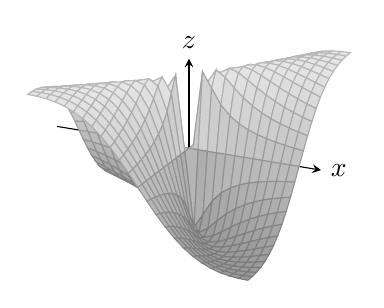
\begin{tikzpicture}[declare function={f(\x,\y)=2*\x*\y/((\x)^2+(\y)^2);}]
  \begin{axis}[small,axis lines=center,colormap={}{gray(0.2cm)=(0.6);gray(1cm)=(0.9);},enlargelimits=true,xlabel={$x$},ylabel={$y$},zlabel={$z$},hide y axis,xlabel style={anchor={west}},zlabel style={anchor=south},xtick={\empty},ytick={\empty},ztick={\empty}]
    \addplot3[surf] { (x==0&&y==0) ?0 : f(x,y) } ;
  \end{axis}
\end{tikzpicture}
\end{subfigure}\hfill
\begin{subfigure}{0.45\textwidth}
\centering
\begin{tikzpicture}[declare function={f(\x,\y)=2*\x*\y/((\x)^2+(\y)^2);}]
  \begin{axis}[small,axis lines=center,colormap={}{gray(0.2cm)=(0.6);gray(1cm)=(0.9);},enlargelimits=true,xlabel={$x$},ylabel={$y$},zlabel={$z$},xlabel style={anchor={west}},ylabel style={anchor=south west},zlabel style={anchor=south},xtick={\empty},ytick={\empty},ztick={\empty},hide z axis]
\addplot3[contour gnuplot={output point meta=rawz,number=5,labels=false,},samples=41,z filter/.code=\def\pgfmathresult{0},]{f(x,y)};
\addplot3[] coordinates {(0,0,0)}coordinate(ka);
  \end{axis}
\draw[fill=white](ka) circle (2pt);
\end{tikzpicture}
\end{subfigure}
\caption{ماسوائے نقطہ \عددی{(0,0)} تفاعل \عددی{f(x,y)} استمراری ہے۔}
\label{شکل_مثال_کثیرالمتغیر_حد_یکتا_ضروری}
\end{figure}

\ابتدا{مثال}\شناخت{مثال_کثیرالمتغیر_حد_یکتا_ضروری}
دکھائیں کہ ماسوائے مبدا   درج ذیل ہر نقطہ پر استمراری ہے (شکل \حوالہ{شکل_مثال_کثیرالمتغیر_حد_یکتا_ضروری})۔
\begin{align*}
f(x,y)=
\begin{cases}
\frac{2xy}{x^2+y^2},&(x,y)\ne (0,0)\\
0,&(x,y)=(0,0)
\end{cases}
\end{align*}
حل:\quad
ہر نقطہ \عددی{(x,y)\ne (0,0)} پر تفاعل کی قیمت \عددی{x} اور \عددی{y}کے  ناطق تفاعل سے حاصل کی جاتی ہے لہٰذا   \عددی{f}   استمراری ہو گا۔

نقطہ \عددی{(0,0)} پر \عددی{f}  کی قیمت معین ہے، لیکن ہم دعویٰ کرتے ہیں کہ \عددی{(x,y)\to(0,0)} کرتے ہوئے اس کا حد غیر موجود ہے۔اس کی وجہ، جیسا ہم دیکھیں گے،   یہ ہے کہ مبدا تک مختلف راہوں سے پہنچتے ہوئے مختلف  نتائج حاصل ہوتے ہیں۔

درج ذیل کی بنا، سوراخ دار لکیر \عددی{y=mx,\, x\ne 0} پر \عددی{m} کی ہر قیمت کے لئے تفاعل \عددی{f} کی ایک مستقل قیمت  ہو گی۔
\begin{align*}
\left. f(x,y)\right\vert_{y=mx}=\left. \frac{2xy}{x^2+y^2}\right\vert_{y=mx}=\frac{2x(mx)}{x^2+(mx)^2}=\frac{2mx^2}{x^2+m^2x^2}=\frac{2m}{1+m^2}
\end{align*}
یوں  اس لکیر  پر جیسے جیسے   \عددی{(x,y)} مبدا تک پہنچتا ہے،  \عددی{f} کی حد اتنی ہو گی:
\begin{align*}
\lim_{\substack{(x,y)\to(0,0)\\ \text{\RL{خط $y=mx$ پر}}}} f(x,y)=\lim_{(x,y)\to(0,0)}\big[\left.f(x,y)\right\vert_{y=mx}\big]=\frac{2m}{1+m^2}
\end{align*}
ہم دیکھتے ہیں کہ حد کی قیمت \عددی{m} پر منحصر ہے۔یوں ایسی کوئی   یکتا قیمت حاصل نہیں ہوتی  جس کو    مبدا تک \عددی{(x,y)} پہنچنے   پر ہم  \عددی{f}  کی حد کہہ سکیں۔ مبدا پر حد غیر موجود ہے لہٰذا مبدا  پر تفاعل غیر استمراری ہو گا۔
\انتہا{مثال}
%=============

دو  (یا دو سے زیادہ)متغیرات کے تفاعل کے حد کے بارے میں ایک اہم نقطہ مثال \حوالہ{مثال_کثیرالمتغیر_حد_یکتا_ضروری} میں  اجاگر ہوا۔ ایک نقطہ پر حد کی موجودگی کے لئے  ضروری ہے کہ اس نقطہ تک  تمام آمد    راہوں  پر  حد  کی قیمت ایک جیسی ہو۔  یوں جب بھی ہم ایک نقطہ  تک  ایسی راہیں  تلاش  کریں جن  پر حد ایک دوسرے سے  مختلف ہوں  تب  اس نقطہ پر تفاعل کا حد غیر موجود ہو گا۔

\ابتدا{پرکھ}\موٹا{حد کی غیر موجودگی کی  دو راہ  پرکھ}\\
اگر \عددی{(x_0,y_0)} تک نقطہ \عددی{(x,y)} ایسی دو مختلف راہوں سے پہنچے جن پر \عددی{f(x,y)} کے حد ایک دوسرے سے مختلف ہوں تب \عددی{\lim\limits_{(x,y)\to(x_0,y_0)}f(x,y)} غیر موجود ہو گا۔
\انتہا{پرکھ}
%===================

\ابتدا{مثال}\شناخت{مثال_کثیرالمتغیر_مبدا_پر_غیر_استمراری_سطح_ب}
دکھائیں کہ \عددی{(0,0)} تک \عددی{(x,y)} پہنچنے سے درج ذیل تفاعل کا کوئی حد حاصل نہیں ہوتا ہے (شکل \حوالہ{شکل_مثال_کثیرالمتغیر_مبدا_پر_غیر_استمراری_سطح_ب})۔
\begin{align*}
f(x,y)=\frac{2x^2y}{x^4+y^2}
\end{align*}
حل:\quad
منحنی \عددی{y=kx^2,\, x\ne 0} پر اس تفاعل کی قیمت ایک مستقل ہے:
\begin{align*}
\left.f(x,y)\right\vert_{y=kx^2}=\left.\frac{2x^2y}{x^4+y^2}\right\vert_{y=kx^2}=\frac{2x^2(kx^2)}{x^4+(kx^2)^2}=\frac{2kx^4}{x^4+k^2x^4}=\frac{2k}{1+k^2}
\end{align*}  
یوں
\begin{align*}
\lim_{\substack{(x,y)\to (0,0)\\ \text{\RL{$y=kx^2$ پر}}}}f(x,y)=\lim_{(x,y)\to(0,0)}\big[\left.f(x,y)\right\vert_{y=kx^2}\big]=\frac{2k}{1+k^2}
\end{align*}
ہو گا  جو   آمد راہ  پر منحصر ہے۔ اگر \عددی{(x,y)} نقطہ \عددی{(0,0)} تک قطع مکافی \عددی{y=x^2}  راہ پر چلتے ہوئے پہنچے، جہاں \عددی{k=1} ہے،  تب حد \عددی{1} کے برابر حاصل ہوتا ہے۔ اگر \عددی{(x,y)} نقطہ \عددی{(0,0)} تک محور \عددی{x} پر چلتے ہوئے پہنچے، جہاں \عددی{k=0} ہے،  تب حد \عددی{0} کے برابر حاصل ہوتا ہے۔ یوں دو راہ پرکھ کے تحت \عددی{(0,0)} تک \عددی{(x,y)} کے پہنچنے سے \عددی{f} کا کوئی حد حاصل نہیں ہو گا۔  
\انتہا{مثال}
%=================
\begin{figure}
\centering
\begin{subfigure}{0.45\textwidth}
\centering
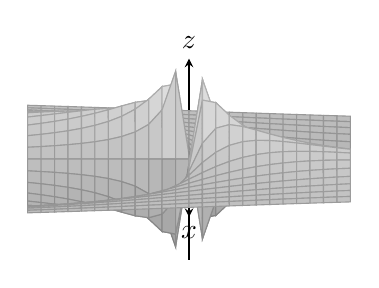
\begin{tikzpicture}[declare function={f(\x,\y)=2*\x*\y/((\x)^4+(\y)^2);}]
  \begin{axis}[view/h=90,small,axis lines=center,colormap={}{gray(0.2cm)=(0.6);gray(1cm)=(0.9);},enlargelimits=true,xlabel={$x$},ylabel={$y$},zlabel={$z$},hide y axis,xlabel style={anchor={north}},zlabel style={anchor=south},xtick={\empty},ytick={\empty},ztick={\empty}]
    \addplot3[surf,domain=-2:2,domain y=-1:1] { (x==0&&y==0) ?0 : f(x,y) } ;
  \end{axis}
\end{tikzpicture}
\end{subfigure}\hfill
\begin{subfigure}{0.45\textwidth}
\centering
\begin{tikzpicture}[declare function={f(\x,\y)=2*\x*\y/((\x)^4+(\y)^2);}]
  \begin{axis}[view/h=90,small,axis lines=center,colormap={kdark}{gray(0.2cm)=(0.6);gray(1cm)=(0.6);},enlargelimits=true,xlabel={$x$},ylabel={$y$},zlabel={$z$},xlabel style={anchor={west}},ylabel style={anchor=south west},zlabel style={anchor=south},xtick={\empty},ytick={\empty},ztick={\empty},hide z axis]
\addplot3[contour gnuplot={output point meta=rawz,number=10,labels=false,},samples=41,z filter/.code=\def\pgfmathresult{0},]{f(x,y)};
  \end{axis}
\end{tikzpicture}
\end{subfigure}
\caption{ماسوائے نقطہ \عددی{(0,0)} تفاعل \عددی{f(x,y)=2x^2y/(x^4+y^2)} استمراری ہے۔}
\label{شکل_مثال_کثیرالمتغیر_مبدا_پر_غیر_استمراری_سطح_ب}
\end{figure}
یہاں آپ سوال اٹھا سکتے ہیں کہ مبدا تک نقطہ \عددی{(x,y)} کے پہنچنے سے بہت سارے مختلف حد ملتے ہیں لہٰذا یہ کہنا درست نہیں کہ \عددی{f} کا حد غیر موجود ہے۔ یہی وہ نقطہ ہے جسے سمجھنا ضروری ہے۔ حد کی تعریف  کہتی ہے کہ حد کی قیمت راہ پر منحصر نہیں ہو سکتی۔

\جزوحصہء{دو سے زیادہ متغیرات کے تفاعل}
دو متغیرات کے تفاعل  کے حد اور استمرار کی تعریف  اور ان  تفاعل کے مجموعہ،  فرق، حاصل ضرب، حاصل تقسیم، طاقت اور مرکب کے بارے میں حاصل نتائج  تین یا تین سے زیادہ متغیرات کے تفاعل کے لئے بھی کارآمد  ہیں۔ درج ذیل تفاعل اپنے پورے دائرہ کار میں استمراری ہیں
\begin{align*}
\ln(x+y+z)\quad \text{اور}\quad \frac{y\sin z}{x-1}
\end{align*} 
اور  درج ذیل طرز کا حد ، جہاں \عددی{N} نقطہ \عددی{(x,y,z)} کو ظاہر کرتا ہے،   حاصل کرنے کے لئے  تفاعل میں نقطہ پر  کیا جاتا ہے۔
\begin{align*}
\lim_{N\to(1,0,-1)}\frac{e^{x+z}}{z^2+\cos\sqrt{xy}}=\frac{e^{1-1}}{(-1)^2+\cos 0}=\frac{1}{2}
\end{align*}

\جزوحصہء{سوالات}
\ابتدا{سوالات}
\موٹا{حد کی قیمت کی تلاش}\\
سوال \حوالہ{سوال_کثیرالمتغیر_حد_قیمت_تلاش_الف} تا سوال \حوالہ{سوال_کثیرالمتغیر_حد_قیمت_تلاش_ب} میں حد کی قیمت تلاش کریں۔

\ابتدا{سوال}\شناخت{سوال_کثیرالمتغیر_حد_قیمت_تلاش_الف}
$\lim\limits_{(x,y)\to(0,0)}\frac{3x^2-y^2+5}{x^2+y^2+2}$
\انتہا{سوال}  
   %======== 
  \ابتدا{جواب}
\wf{\unexpanded{
$\tfrac{5}{2}$
}}
\انتہا{جواب}
%==================
\ابتدا{سوال}
$\lim\limits_{(x,y)\to(0,4)}\frac{x}{\sqrt{y}}$
\انتہا{سوال}
%===================
\ابتدا{سوال}
$\lim\limits_{(x,y)\to(3,4)}\sqrt{x^2+y^2-1}$
\انتہا{سوال}  
   %======== 
  \ابتدا{جواب}
\wf{\unexpanded{
$2\sqrt{6}$
}}
\انتہا{جواب}
%===================
\ابتدا{سوال}
$\lim\limits_{(x,y)\to(2,-3)}\big(\frac{1}{x}+\frac{1}{y}\big)^2$
\انتہا{سوال}
%===================
\ابتدا{سوال}
$\lim\limits_{(x,y)\to(0,\pi/4)}\sec x\tan y$
\انتہا{سوال}  
   %======== 
  \ابتدا{جواب}
\wf{\unexpanded{
$1$
}}
\انتہا{جواب}
%===================
\ابتدا{سوال}
$\lim\limits_{(x,y)\to(0,0)}\cos\frac{x^2+y^3}{x+y+1}$
\انتہا{سوال}
%===================
\ابتدا{سوال}
$\lim\limits_{(x,y)\to(0,\ln 2)}e^{x-y}$
\انتہا{سوال}  
   %======== 
  \ابتدا{جواب}
\wf{\unexpanded{
$\tfrac{1}{2}$
}}
\انتہا{جواب}
%===================
\ابتدا{سوال}
$\lim\limits_{(x,y)\to(1,1)}\ln\abs{1+x^2y^2}$
\انتہا{سوال}
%===================
\ابتدا{سوال}
$\lim\limits_{(x,y)\to(0,0)} \frac{e^y\sin x}{x}$
\انتہا{سوال}  
   %======== 
  \ابتدا{جواب}
\wf{\unexpanded{
$1$
}}
\انتہا{جواب}
%===================
\ابتدا{سوال}
$\lim\limits_{(x,y)\to(1,1)}\cos\sqrt[3]{\abs{xy}-1}$
\انتہا{سوال}
%===================
\ابتدا{سوال}
$\lim\limits_{(x,y)\to(1,0)}\frac{x\sin y}{x^2+1}$
\انتہا{سوال}  
   %======== 
  \ابتدا{جواب}
\wf{\unexpanded{
$0$
}}
\انتہا{جواب}
%===================
\ابتدا{سوال}\شناخت{سوال_کثیرالمتغیر_حد_قیمت_تلاش_ب}
$\lim\limits_{(x,y)\to(\pi/2,0)}\frac{\cos y+1}{y-\sin x}$
\انتہا{سوال}
%===================

\موٹا{حاصل تقسیم کے حد}\\
حاصل تقسیم کو ترتیب دیتے ہوئے سوال \حوالہ{سوال_کثیرالمتغیر_ترتیب_حد_تلاش_الف} تا سوال \حوالہ{سوال_کثیرالمتغیر_ترتیب_حد_تلاش_ب} میں حد تلاش کریں۔

\ابتدا{سوال}\شناخت{سوال_کثیرالمتغیر_ترتیب_حد_تلاش_الف}
$\lim\limits_{\substack{(x,y)\to(1,1)\\ x\ne y}}\frac{x^2-2xy+y^2}{x-y}$
\انتہا{سوال}  
   %======== 
  \ابتدا{جواب}
\wf{\unexpanded{
$0$
}}
\انتہا{جواب}
%=================
\ابتدا{سوال}
$\lim\limits_{\substack{(x,y)\to(1,1)\\ x\ne y}}\frac{x^2-y^2}{x-y}$
\انتہا{سوال}
%=================
\ابتدا{سوال}
$\lim\limits_{\substack{(x,y)\to(1,1)\\x\ne 1}}\frac{xy-y-2x+2}{x-1}$
\انتہا{سوال}  
   %======== 
  \ابتدا{جواب}
\wf{\unexpanded{
$-1$
}}
\انتہا{جواب}
%=================
\ابتدا{سوال}
$\lim\limits_{\substack{(x,y)\to(2,-4)\\y\ne -4,\, x\ne x^2}}\frac{y+4}{x^2y-xy+4x^2-4x}$
\انتہا{سوال}
%=================
\ابتدا{سوال}
$\lim\limits_{\substack{(x,y)\to(0,0)\\x\ne y}}\frac{x-y+2\sqrt{x}-2\sqrt{y}}{\sqrt{x}-\sqrt{y}}$
\انتہا{سوال}  
   %======== 
  \ابتدا{جواب}
\wf{\unexpanded{
$2$
}}
\انتہا{جواب}
%=================
\ابتدا{سوال}
$\lim\limits_{\substack{(x,y)\to(2,2)\\x+y\ne 4}}\frac{x+y-4}{\sqrt{x+y}-2}$
\انتہا{سوال}
%=================
\ابتدا{سوال}
$\lim\limits_{\substack{(x,y)\to(2,0)\\2x-y\ne 4}}\frac{\sqrt{2x-y}-2}{2x-y-4}$
\انتہا{سوال}  
   %======== 
  \ابتدا{جواب}
\wf{\unexpanded{
$\tfrac{1}{4}$
}}
\انتہا{جواب}
%=================
\ابتدا{سوال}\شناخت{سوال_کثیرالمتغیر_ترتیب_حد_تلاش_ب}
$\lim\limits_{\substack{(x,y)\to(4,3)\\x\ne y+1}}\frac{\sqrt{x}-\sqrt{y+1}}{x-y-1}$
\انتہا{سوال}
%=================

\موٹا{تین متغیرات کے تفاعل کا حد}\\
سوال \حوالہ{سوال_کثیرالمتغیر_تین_متغیر_حد_الف} تا سوال \حوالہ{سوال_کثیرالمتغیر_تین_متغیر_حد_ب} میں حد تلاش کریں۔

\ابتدا{سوال}\شناخت{سوال_کثیرالمتغیر_تین_متغیر_حد_الف}
$\lim\limits_{N\to (1,3,4)}\big(\frac{1}{x}+\frac{1}{y}+\frac{1}{z}\big)$
\انتہا{سوال}  
   %======== 
  \ابتدا{جواب}
\wf{\unexpanded{
$\tfrac{19}{12}$
}}
\انتہا{جواب}
%=====================
\ابتدا{سوال}
$\lim\limits_{N\to(1,-1,-1)}\frac{2xy+yz}{x^2+z^2}$
\انتہا{سوال}
%================
\ابتدا{سوال}
$\lim\limits_{N\to(3,3,0)}(\sin^2x+\cos^2y+\sec^2z)$
\انتہا{سوال}  
   %======== 
  \ابتدا{جواب}
\wf{\unexpanded{
$2$
}}
\انتہا{جواب}
%======================
\ابتدا{سوال}
$\lim\limits_{N\to(-1/4,\pi/2,2)}\tan^{-1}xyz$
\انتہا{سوال}
%======================
\ابتدا{سوال}
$\lim\limits_{N\to(\pi,0,3)}ze^{-2y}\cos 2x$
\انتہا{سوال}  
   %======== 
  \ابتدا{جواب}
\wf{\unexpanded{
$3$
}}
\انتہا{جواب}
%======================
\ابتدا{سوال}\شناخت{سوال_کثیرالمتغیر_تین_متغیر_حد_ب}
$\lim\limits_{N\to(0,-2,0)}\ln\sqrt{x^2+y^2+z^2}$
\انتہا{سوال}
%======================

\موٹا{مستوی میں استمرار}\\
سوال \حوالہ{سوال_کثیرالمتغیر_استمراری_سطح_الف} تا سوال \حوالہ{سوال_کثیرالمتغیر_استمراری_سطح_ب} میں  کس نقطہ \عددی{(x,y)} پر مستوی میں تفاعل استمراری ہیں؟

\ابتدا{سوال}\شناخت{سوال_کثیرالمتغیر_استمراری_سطح_الف}
(ا)
$f(x,y)=\sin(x+y)$\quad
(ب)
$f(x,y)=\ln(x^2+y^2)$
\انتہا{سوال}  
   %======== 
  \ابتدا{جواب}
\wf{\unexpanded{
(ا)   تمام \عددی{(x,y)}، (ب) ماسوائے \عددی{(0,0)} تمام \عددی{(x,y)}
}}
\انتہا{جواب}
%==================
\ابتدا{سوال}
(ا)
$f(x,y)=\frac{x+y}{x-y}$\quad
(ب)
$f(x,y)=\frac{y}{x^2+1}$
\انتہا{سوال}
%=================
\ابتدا{سوال}
(ا)
$g(x,y)=\sin\frac{1}{xy}$\quad
(ب)
$g(x,y)=\frac{x+y}{2+\cos x}$
\انتہا{سوال}  
   %======== 
  \ابتدا{جواب}
\wf{\unexpanded{
(ا) تمام \عددی{(x,y)} ماسوائے جہاں \عددی{x=0} یا \عددی{y=0} ہو، (ب) تمام \عددی{(x,y)}
}}
\انتہا{جواب}
%=================
\ابتدا{سوال}\شناخت{سوال_کثیرالمتغیر_استمراری_سطح_ب}
(ا)
$g(x,y)=\frac{x^2+y^2}{x^2-3x+2}$\quad
(ب)
$g(x,y)=\frac{1}{x^2-y}$
\انتہا{سوال}
%=================

\موٹا{فضا میں استمرار}\\
سوال \حوالہ{سوال_کثیرالمتغیر_استمراری_فضا_الف} تا سوال \حوالہ{سوال_کثیرالمتغیر_استمراری_فضا_ب} میں  کس نقطہ \عددی{(x,y,z)} پر فضا  میں تفاعل استمراری ہیں؟

\ابتدا{سوال}\شناخت{سوال_کثیرالمتغیر_استمراری_فضا_الف}
(ا)
$f(x,y,z)=x^2+y^2-2z^2$\quad
(ب)
$f(x,y,z)=\sqrt{x^2+y^2-1}$
\انتہا{سوال}  
   %======== 
  \ابتدا{جواب}
\wf{\unexpanded{
(ا) تمام \عددی{(x,y,z)}، (ب) نلکی \عددی{x^2+y^2=1} کی اندرون کے علاوہ تمام \عددی{(x,y,z)}
}}
\انتہا{جواب}
%=================
\ابتدا{سوال}
(ا)
$f(x,y,z)=\ln xyz$\quad
(ب)
$f(x,y,z)=e^{x+y}\cos z$
\انتہا{سوال}
%=====================
\ابتدا{سوال}
(ا)
$h(x,y,z)=xy\sin\frac{1}{z}$\quad
(ب)
$h(x,y,z)=\frac{1}{x^2+z^2-1}$
\انتہا{سوال}  
   %======== 
  \ابتدا{جواب}
\wf{\unexpanded{
(ا) وہ تمام \عددی{(x,y,z)} جہاں \عددی{z\ne 0} ہو، (ب)   وہ تمام \عددی{(x,y,z)} جہاں \عددی{x^2+y^2\ne 1} ہو۔
}}
\انتہا{جواب}
%=====================
\ابتدا{سوال}\شناخت{سوال_کثیرالمتغیر_استمراری_فضا_ب}
(ا)
$h(x,y,z)=\frac{1}{\abs{y}+\abs{z}}$\quad
(ب)
$h(x,y,z)=\frac{1}{\abs{xy}+\abs{z}}$
\انتہا{سوال}
%=====================

\موٹا{نقطہ پر حد غیر موجود}\\
نقطہ تک   مختلف راہ پر پہنچتے ہوئے سوال \حوالہ{سوال_کثیرالمتغیر_غیر_موجود_حد_الف} تا سوال \حوالہ{سوال_کثیرالمتغیر_غیر_موجود_حد_ب} میں دکھائیں کہ \عددی{(x,y)\to(0,0)} کرتے ہوئے تفاعل کا کوئی حد نہیں پایا جاتا ہے۔

\ابتدا{سوال}\شناخت{سوال_کثیرالمتغیر_غیر_موجود_حد_الف}
$f(x,y)=-\frac{x}{\sqrt{x^2+y^2}}$\quad
(شکل \حوالہ{شکل_سوال_کثیرالمتغیر_غیر_موجود_حد_الف}-ا)
\انتہا{سوال}  
   %======== 
  \ابتدا{جواب}
\wf{\unexpanded{
راہ \عددی{y=x,x>0} اور \عددی{y=x,x<0}  لیں۔ 
}}
\انتہا{جواب}
%===================
\begin{figure}
\centering
\begin{subfigure}{0.45\textwidth}
\centering
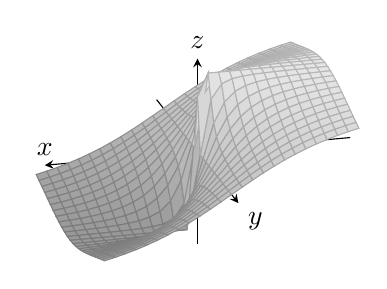
\begin{tikzpicture}[declare function={f(\x,\y)=-\x/sqrt((\x)^2+(\y)^2);}]
\begin{axis}[small,axis lines=center,view/h=165,colormap={}{gray(0.2cm)=(0.6);gray(1cm)=(0.9);},enlargelimits=true,xlabel={$x$},ylabel={$y$},zlabel={$z$},xlabel style={anchor=south},ylabel style={anchor=north west},zlabel style={anchor=south},xtick={\empty},ytick={\empty},ztick={\empty}]
\addplot3[z buffer=sort,surf,domain=-0.1:0.1,domain y=-0.1:0.1]{f(x,y)};
\end{axis}
\end{tikzpicture}
\caption{}
\end{subfigure}\hfill
\begin{subfigure}{0.45\textwidth}
\centering
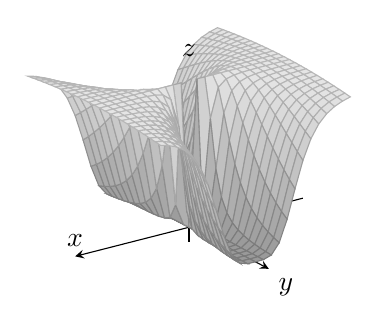
\begin{tikzpicture}[declare function={f(\x,\y)=(\x)^4/((\x)^4+(\y)^2);}]
\begin{axis}[small,axis lines=center,view/h=145,colormap={}{gray(0.2cm)=(0.6);gray(1cm)=(0.9);},enlargelimits=true,xlabel={$x$},ylabel={$y$},zlabel={$z$},xlabel style={anchor=south},ylabel style={anchor=north west},zlabel style={anchor=south},xtick={\empty},ytick={\empty},ztick={\empty}]
\addplot3[z buffer=sort,surf]{f(x,y)};
\end{axis}
\end{tikzpicture}
\caption{}
\end{subfigure}
\caption{}
\label{شکل_سوال_کثیرالمتغیر_غیر_موجود_حد_الف}
\end{figure}
\ابتدا{سوال}
$h(x,y)=\frac{x^4}{x^4+y^2}$\quad
(شکل \حوالہ{شکل_سوال_کثیرالمتغیر_غیر_موجود_حد_الف}-ب)
\انتہا{سوال}
%=================
\ابتدا{سوال}
$h(x,y)=\frac{x^4-y^2}{x^4+y^2}$
\انتہا{سوال}  
   %======== 
  \ابتدا{جواب}
\wf{\unexpanded{
راہ \عددی{y=kx^2} لیں جہاں \عددی{k} ایک  مستقل ہو۔
}}
\انتہا{جواب}
%================
\ابتدا{سوال}
$f(x,y)=\frac{xy}{\abs{xy}}$
\انتہا{سوال}
%=================
\ابتدا{سوال}
$g(x,y)=\frac{x-y}{x+y}$
\انتہا{سوال}  
   %======== 
  \ابتدا{جواب}
\wf{\unexpanded{
راہ \عددی{y=mx} لیں جہاں \عددی{m} ایک مستقل    \عددی{m\ne -1} ہو۔
}}
\انتہا{جواب}
%=================
\ابتدا{سوال}
$g(x,y)=\frac{x+y}{x-y}$
\انتہا{سوال}
%=================
\ابتدا{سوال}
$h(x,y)=\frac{x^2+y}{y}$
\انتہا{سوال}  
   %======== 
  \ابتدا{جواب}
\wf{\unexpanded{
راہ \عددی{y=kx^2} لیں جہاں \عددی{k} ایک مستقل  \عددی{k\ne 0} ہو۔ 
}}
\انتہا{جواب}
%=================
\ابتدا{سوال}\شناخت{سوال_کثیرالمتغیر_غیر_موجود_حد_ب}
$h(x,y)=\frac{x^2}{x^2-y}$
\انتہا{سوال}
%=================
\موٹا{نظریہ اور مثالیں}\\
\ابتدا{سوال}
کیا  \عددی{\lim_{(x,y)\to(x_0,y_0)}f(x,y)=L} کی صورت میں \عددی{(x_0,y_0)} کا معین ہونا لازمی ہے؟ اپنے جواب کی وجہ پیش کریں۔
\انتہا{سوال}  
   %======== 
  \ابتدا{جواب}
\wf{\unexpanded{
نہیں
}}
\انتہا{جواب}
%=====================
\ابتدا{سوال}
اگر \عددی{f(x_0,y_0)=3} ہو تب درج ذیل کے بارے میں  (ا)   \عددی{(x_0,y_0)} پر استمراری \عددی{f} کی صورت میں،
\begin{align*}
\lim_{(x,y)\to(x_0,y_0)} f(x,y)
\end{align*}
(ب)  \عددی{(x_0,y_0)} پر غیر استمراری \عددی{f} کی صورت میں کیا کہا جا  سکتا ہے۔ اپنے جواب کہ وجہ پیش کریں۔
\انتہا{سوال}
%===============
دو متغیرات کے تفاعل کا مسئلہ بیچ  کہتا ہے کہ اگر ایک قرص، جس کا  مرکز  \عددی{(x_0,y_0)} ہو، کے اندر تمام \عددی{(x,y)\ne (x_0,y_0)} پر \عددی{g(x,y)\le f(x,y)\le h(x,y)} ہو،  اور \عددی{(x,y)\to (x_0,y_0)} کرتے ہوئے  \عددی{g} اور \عددی{h} دونوں کا  حد  متناہی اور \عددی{L} ہو   تب
\begin{align*}
\lim_{(x,y)\to(x_0,y_0)}f(x,y)=L
\end{align*}
ہو گا۔سوال \حوالہ{سوال_کثیرالمتغیر_مسئلہ_بیچ_الف} تا سوال \حوالہ{سوال_کثیرالمتغیر_مسئلہ_بیچ_ب} میں  اس نتیجہ  کا سہارا لیتے ہوئے جواب دیں۔ 

\ابتدا{سوال}\شناخت{سوال_کثیرالمتغیر_مسئلہ_بیچ_الف}
کیا 
\begin{align*}
1-\frac{x^2y^2}{3}<\frac{\tan^{-1}xy}{xy}<1
\end{align*}
جانتے ہوئے آپ
\begin{align*}
\lim\limits_{(x,y)\to(0,0)}\frac{\tan^{-1}xy}{xy}
\end{align*}
کے بارے میں کچھ کہہ سکتے ہیں؟ اپنے جواب کی وجہ پیش کریں۔
\انتہا{سوال}  
   %======== 
  \ابتدا{جواب}
\wf{\unexpanded{
حد \عددی{1} ہے۔
}}
\انتہا{جواب}
%============
\ابتدا{سوال}
کیا
\begin{align*}
2\abs{xy}-\frac{x^2y^2}{6}<4-4\cos\sqrt{\abs{xy}}<2\abs{xy}
\end{align*}
جانتے ہوئے
\begin{align*}
\lim\limits_{(x,y)\to(0,0)}\frac{4-4\cos\sqrt{\abs{xy}}}{\abs{xy}}
\end{align*}
کے بارے میں کچھ کہا جا سکتا ہے؟ اپنے جواب کی وجہ پیش کریں۔
\انتہا{سوال}
%===============
\ابتدا{سوال}
کیا \عددی{\abs{\sin(1/x)}\le 1} جانتے ہوئے درج ذیل کے بارے میں کچھ کہا جا سکتا ہے؟ اپنے جواب کی وجہ پیش کریں۔
\begin{align*}
\lim\limits_{(x,y)\to(0,0)}y\sin\frac{1}{x}
\end{align*}
\انتہا{سوال}  
   %======== 
  \ابتدا{جواب}
\wf{\unexpanded{
حد \عددی{0} ہے۔
}}
\انتہا{جواب}
%==============
\ابتدا{سوال}
کیا \عددی{\abs{\cos(1/y)}\le 1} جانتے ہوئے درج ذیل کے بارے میں کچھ کہا جا سکتا ہے؟ اپنے جواب کی وجہ پیش کریں۔
\begin{align*}
\lim\limits_{(x,y)\to(0,0)}x\cos\frac{1}{y}
\end{align*}
\انتہا{سوال}
%==============
\ابتدا{سوال}
(ا)دوبارہ  مثال \حوالہ{مثال_کثیرالمتغیر_حد_یکتا_ضروری} کو  پڑھیں۔اب درج ذیل کلیہ میں \عددی{m=\tan\theta} پر کر کے اس کی سادہ صورت حاصل کرتے ہوئے دکھائیں کہ \عددی{f} کی قیمت  لکیر کے زاویہ میلان  پر منحصر ہی گی۔
\begin{align*}
\left.f(x,y)\right\vert_{y=mx}=\frac{2m}{1+m^2}
\end{align*}
(ب) جزو-ا میں حاصل کلیہ استعمال کرتے ہوئے دکھائیں کہ لکیر \عددی{y=mx} پر چلتے ہوئے \عددی{(x,y)\to (0,0)} کرنے سے \عددی{f} کے  حد کی قیمت \عددی{-1} تا \عددی{1} ہو سکتی ہے جو قریب پہنچنے کی راہ کے  زاویہ پر منحصر ہو گی۔  
\انتہا{سوال}  
   %======== 
  \ابتدا{جواب}
\wf{\unexpanded{
(ا) \عددی{\left. f(x,y)\right\vert_{y=mx}=\sin2\theta} جہاں\\  
 \عددی{\tan\theta=m} ہے۔
}}
\انتہا{جواب}
%=================
\ابتدا{سوال}\شناخت{سوال_کثیرالمتغیر_مسئلہ_بیچ_ب}
\عددی{f(0,0)} کی ایسی تعریف پیش کریں جو درج ذیل کو مبدا پر بھی استمراری بناتا ہو۔
\begin{align*}
f(x,y)=xy\frac{x^2-y^2}{x^2+y^2}
\end{align*}
\انتہا{سوال}
%==============

\موٹا{قطبی محدد میں تبادلہ}\\
اگر کارتیسی محدد میں \عددی{\lim_{(x,y)\to(0,0)}f(x,y)}  کے حصول میں پیش رفت  نہ ہو تب قطبی محدد میں حد تلاش کرنے کی کوشش کریں۔ ایسا کرنے  کی خاطر \عددی{x=r\cos\theta} اور \عددی{y=r\sin\theta} کرتے ہوئے \عددی{r\to 0}  کے لئے حاصل تفاعل کا حد تلاش کریں۔دوسرے الفاظ میں یہ دیکھنے کی کوشش کریں کہ آیا کوئی ایسا عدد \عددی{L} پایا جاتا ہے جو درج ذیل کو مطمئن کرتا ہو:

کسی بھی دیے گئے عدد \عددی{\epsilon>0} کا ایسا مطابقتی عدد \عددی{\delta>0} پایا جاتا ہو کہ تمام \عددی{r} اور \عددی{\theta} کے لئے درج ذیل ہو۔
\begin{align*}
\abs{r}<\delta\implies \abs{f(r,\theta)-L}<\epsilon
\end{align*}
اگر ایسا \عددی{L} موجود ہو تب
\begin{align}\label{مساوات_کثیرالمتغیر_قطبی_حد_الف}
\lim_{(x,y)\to(0,0)}f(x,y)=\lim_{r\to 0}f(r,\theta)=L
\end{align}
ہو گا۔مثال کے طور پر 
\begin{align*}
\lim_{(x,y)\to(0,0)}\frac{x^3}{x^2+y^2}=\lim_{r\to 0}\frac{r^3\cos^3\theta}{r^2}=\lim_{r\to 0}r\cos^3\theta=0
\end{align*}
ہو گا۔ آخری عدم مساوات  کی تصدیق کرنے کی خاطر ہمیں دکھانا  ہو گا کہ \عددی{f(r,\theta)=r\cos^3\theta} اور \عددی{L}  مساوات \حوالہ{مساوات_کثیرالمتغیر_قطبی_حد_الف} کو مطمئن کرتے ہیں۔ یعنی ہمیں دکھانا ہو گا کہ کسی بھی دیے گئے عدد \عددی{\epsilon>0} کے لئے ایسا مطابقتی  عدد \عددی{\delta>0} موجود ہے کہ  تمام \عددی{r} اور \عددی{\theta} کے لئے درج ذیل  مطمئن ہو۔
\begin{align}\label{مساوات_کثیرالمتغیر_قطبی_حد_ب}
\abs{r}<\delta\implies \abs{r\cos^3\theta-0}<\epsilon
\end{align}
چونکہ
\begin{align*}
\abs{r\cos^3\theta}=\abs{r}\abs{\cos^3\theta}\le \abs{r}\cdot 1=\abs{r}
\end{align*}
ہوتا ہے لہٰذا  \عددی{\delta=\epsilon} لینے سے تمام \عددی{r} اور \عددی{\theta} کے لئے مساوات \حوالہ{مساوات_کثیرالمتغیر_قطبی_حد_ب} مطمئن ہو گا۔

اس کے برعکس    \عددی{\abs{r}} جتنا بھی چھوٹا کیوں نا ہو   درج ذیل تفاعل کی قیمت \عددی{0}  سے  \عددی{1} تک ہو سکتی ہے لہٰذا \عددی{\lim_{(x,y)\to (0,0)}\tfrac{x^2}{x^2+y^2}} غیر موجود ہو گا۔
\begin{align*}
\frac{x^2}{x^2+y^2}=\frac{r^2\cos^2\theta}{r^2}=\cos^2\theta
\end{align*}

درج بالا دو تفاعل میں \عددی{r\to 0} کرتے ہوئے  حد کی موجودگی یا غیر موجودگی کا مسئلہ سیدھا تھا۔البتہ ضروری نہیں کہ  قطبی محدد میں تبادلہ سودمند ثابت ہو، بلکہ بعض اوقات ایسا کرنے سے ہم بالکل غلط نتیجہ کی طرف راغب ہو سکتے ہیں۔ مثال کے طور پر، تمام سیدھے خطوط \عددی{\theta=c}، جہاں \عددی{c} مستقل ہے، پر حد موجود ہو سکتا ہے اگرچہ وسیع معنوں میں حد غیر موجود ہو گا۔ مثال \حوالہ{مثال_کثیرالمتغیر_مبدا_پر_غیر_استمراری_سطح_ب} میں اس حقیقت کی وضاحت کی گئی ہے۔قطبی محدد میں \عددی{r\ne 0} کے لئے  \عددی{f(x,y)=\tfrac{2x^2y}{x^4+y^2}} درج ذیل ہو گا۔
\begin{align*}
f(r\cos\theta,r\sin\theta)=\frac{r\cos\theta\sin2\theta}{r^2\cos^4\theta+\sin^2\theta}
\end{align*}
اب \عددی{\theta}  برقرار رکھتے ہوئے  \عددی{r\to 0} کرنے سے حد \عددی{0} ملتا ہے۔البتہ راہ \عددی{y=x^2} پر \عددی{r\sin\theta=r^2\cos^2\theta}لہٰذا درج ذیل ہو گا۔
\begin{align*}
f(r\cos\theta,r\sin\theta)&=\frac{r\cos\theta\sin 2\theta}{r^2\cos^4\theta+(r\cos^2\theta)^2}\\
&=\frac{2r\cos^2\theta\sin\theta}{2r^2\cos^4\theta}=\frac{r\sin\theta}{r^2\cos^2\theta}=1
\end{align*}

سوال \حوالہ{سوال_کثیرالمتغیر_قطبی_محدد_حد_الف} تا سوال \حوالہ{سوال_کثیرالمتغیر_قطبی_محدد_حد_ب} میں \عددی{(x,y)\to(0,0)} کرتے ہوئے \عددی{f} کا حد تلاش کریں یا دکھائیں کہ اس کا حد غیر موجود ہے۔

\ابتدا{سوال}\شناخت{سوال_کثیرالمتغیر_قطبی_محدد_حد_الف}
$f(x,y)=\frac{x^3-xy^2}{x^2+y^2}$
\انتہا{سوال}  
   %======== 
  \ابتدا{جواب}
\wf{\unexpanded{
$0$
}}
\انتہا{جواب}
%==================
\ابتدا{سوال}
$f(x,y)=\cos\big(\frac{x^3-y^3}{x^2+y^2}\big)$
\انتہا{سوال}
%====================
\ابتدا{سوال}
$f(x,y)=\frac{y^2}{x^2+y^2}$
\انتہا{سوال}  
   %======== 
  \ابتدا{جواب}
\wf{\unexpanded{
غیر موجود ہے۔
}}
\انتہا{جواب}
%====================
\ابتدا{سوال}
$f(x,y)=\frac{2x}{x^2+x+y^2}$
\انتہا{سوال}
%====================
\ابتدا{سوال}
$f(x,y)=\tan^{-1}\big(\frac{\abs{x}+\abs{y}}{x^2+y^2}\big)$
\انتہا{سوال}  
   %======== 
  \ابتدا{جواب}
\wf{\unexpanded{
$\tfrac{\pi}{2}$
}}
\انتہا{جواب}
%====================
\ابتدا{سوال}\شناخت{سوال_کثیرالمتغیر_قطبی_محدد_حد_ب}
$f(x,y)=\frac{x^2-y^2}{x^2+y^2}$
\انتہا{سوال}
%====================

سوال \حوالہ{سوال_کثیرالمتغیر_مبدا_پر_استمراری_الف} اور سوال \حوالہ{سوال_کثیرالمتغیر_مبدا_پر_استمراری_ب} میں \عددی{f(0,0)} کی ایسی تعریف پیش کریں کہ \عددی{f} مبدا پر بھی استمراری ہو۔

\ابتدا{سوال}\شناخت{سوال_کثیرالمتغیر_مبدا_پر_استمراری_الف}
$f(x,y)=\ln\big(\frac{3x^2-x^2y^2+3y^2}{x^2+y^2}\big)$
\انتہا{سوال}  
   %======== 
  \ابتدا{جواب}
\wf{\unexpanded{
$f(0,0)=\ln 3$
}}
\انتہا{جواب}
%====================
\ابتدا{سوال}\شناخت{سوال_کثیرالمتغیر_مبدا_پر_استمراری_ب}
$f(x,y)=\frac{2xy^2}{x^2+y^2}$
\انتہا{سوال}
%=================

\موٹا{\عددی{\delta\epsilon}  تعریفات  کا استعمال}\\
\ابتدا{سوال}
دکھائیں کہ حد کی تعریف  (مساوات \حوالہ{مساوات_کثیرالمتغیر_تعریف_حد_الف}) میں \عددی{\delta\epsilon} پر عائد  شرط مساوات \حوالہ{مساوات_کثیرالمتغیر_تعریف_حد_ب} میں دی گئی شرط کے مترادف ہے۔
\انتہا{سوال}
%===================
\ابتدا{سوال}
\عددی{(x,y)\to (x_0,y_0)} کرتے ہوئے تفاعل \عددی{f(x,y)}کے حد  کی باضابطہ \عددی{\delta\epsilon} تعریف کو مد نظر رکھتے ہوئے  \عددی{(x,y,z)\to(x_ 0,y_0,z_0)} کرتے ہوئے \عددی{g(x,y,z)} کے حد کی تعریف پیش کریں۔چار غیر تابع متغیرات کے تفاعل \عددی{h(x,y,z,t)} کی حد کی تعریف کیا ہو گی؟  
\انتہا{سوال}
%=========

سوال \حوالہ{سوال_کثیرالمتغیر_حد_دو_متغیرات_الف} تا سوال \حوالہ{سوال_کثیرالمتغیر_حد_دو_متغیرات_ب} میں  تفاعل \عددی{f(x,y)} اور مثبت عدد \عددی{\epsilon} دیے گئے ہیں۔ ہر ایک سوال میں یا دکھائیں کہ  ایسا \عددی{\delta>0} موجود ہے  کہ  \عددی{(x,y)} کے لئے 
\begin{align*}
\sqrt{x^2+y^2}<\delta\implies \abs{f(x,y)-f(0,0)}<\epsilon
\end{align*}
مطمئن ہوتا ہے  یا دکھائیں کہ ایسا \عددی{\delta>0} موجود ہے کہ تمام \عددی{(x,y)} کے لئے
\begin{align*}
\abs{x}<\delta,\quad \abs{y}<\delta \implies \abs{f(x,y)-f(0,0)}<\epsilon
\end{align*}
مطمئن ہوتا ہے۔ان میں سے وہ دکھائیں  جو آپ کو زیادہ  آسان لگے۔ دونوں دکھانے  کی ضرورت نہیں ہے۔ 

\ابتدا{سوال}\شناخت{سوال_کثیرالمتغیر_حد_دو_متغیرات_الف}
$f(x,y)=x^2+y^2,\quad \epsilon=0.01$
\انتہا{سوال}  
   %======== 
  \ابتدا{جواب}
\wf{\unexpanded{
$\delta=0.1$
}}
\انتہا{جواب}
%==================
\ابتدا{سوال}
$f(x,y)=\frac{y}{x^2+1},\quad \epsilon=0.05$
\انتہا{سوال}
%==============
\ابتدا{سوال}
$f(x,y)=\frac{x+y}{x^2+1},\quad \epsilon=0.01$
\انتہا{سوال}  
   %======== 
  \ابتدا{جواب}
\wf{\unexpanded{
$\delta=0.005$
}}
\انتہا{جواب}
%================
\ابتدا{سوال}\شناخت{سوال_کثیرالمتغیر_حد_دو_متغیرات_ب}
$f(x,y)=\frac{x+y}{2+\cos x},\quad \epsilon=0.02$
\انتہا{سوال}
%=================


سوال \حوالہ{سوال_کثیرالمتغیر_حد_تین_متغیرات_الف} تا سوال \حوالہ{سوال_کثیرالمتغیر_حد_تین_متغیرات_ب} میں  تفاعل \عددی{f(x,y,z)} اور مثبت عدد \عددی{\epsilon} دیے گئے ہیں۔ ہر ایک سوال میں یا دکھائیں کہ  ایسا \عددی{\delta>0} موجود ہے  کہ  \عددی{(x,y,z)} کے لئے 
\begin{align*}
\sqrt{x^2+y^2+z^2}<\delta\implies \abs{f(x,y,z)-f(0,0,0)}<\epsilon
\end{align*}
مطمئن ہوتا ہے  یا دکھائیں کہ ایسا \عددی{\delta>0} موجود ہے کہ تمام \عددی{(x,y,z)} کے لئے
\begin{align*}
\abs{x}<\delta,\quad \abs{y}<\delta,\quad \abs{z}<\delta  \implies \abs{f(x,y,z)-f(0,0,0)}<\epsilon
\end{align*}
مطمئن ہوتا ہے۔ان میں سے وہ دکھائیں  جو آپ کو زیادہ  آسان لگے۔ دونوں دکھانے کی ضرورت نہیں ہے۔ 

\ابتدا{سوال}\شناخت{سوال_کثیرالمتغیر_حد_تین_متغیرات_الف}
$f(x,y,z)=x^2+y^2+z^2,\quad \epsilon=0.015$
\انتہا{سوال}  
   %======== 
  \ابتدا{جواب}
\wf{\unexpanded{
$\delta=\sqrt{0.015}$
}}
\انتہا{جواب}
%=================
\ابتدا{سوال}
$f(x,y,z)=xyz,\quad \epsilon=0.008$
\انتہا{سوال}
%===================
\ابتدا{سوال}
$f(x,y,z)=\frac{x+y+z}{x^2+y^2+z^2+1},\quad \epsilon=0.015$
\انتہا{سوال}  
   %======== 
  \ابتدا{جواب}
\wf{\unexpanded{
$\delta=0.005$
}}
\انتہا{جواب}
%===================
\ابتدا{سوال}\شناخت{سوال_کثیرالمتغیر_حد_تین_متغیرات_ب}
$f(x,y,z)=\tan^2x+\tan^2y+\tan^2z,\quad \epsilon=0.03$
\انتہا{سوال}
%===================
\ابتدا{سوال}
دکھائیں کہ ہر نقطہ  \عددی{(x_0,y_0,z_0)} پر تفاعل \عددی{f(x,y,z)=x+y-z} استمراری ہے۔ 
\انتہا{سوال}
%===============
\ابتدا{سوال}
دکھائیں کہ مبدا پر \عددی{f(x,y,z)=x^2+y^2+z^2} استمراری ہے۔
\انتہا{سوال}
%==================
\انتہا{سوالات}


\حصہ{جزوی تفرقات}
جب ہم   ماسوائے ایک غیر تابع متغیر  کے باقی تمام  کو برقرار رکھیں اور اس ایک متغیر کے لحاظ سے تفاعل کا تفرق لیں تو ہمیں "جزوی" تفرق حاصل ہوتا ہے۔ اس حصہ میں دکھایا جائے گا کہ جزوی تفرقات کیسے  پائے جاتے ہیں اور واحد متغیر کے تفاعل کے تفرق کے قواعد بروئے کار لاتے ہوئے   جزوی تفرقات   کی قیمت کے حصول کے بارے میں بتایا جائے گا۔

\جزوحصہء{تعریفات اور علامتیت }
اگر تفاعل \عددی{f(x,y)} کے دائرہ کار میں \عددی{(x_0,y_0)} ایک نقطہ ہو تب انتصابی سطح \عددی{y=y_0}  سطح \عددی{z=f(x,y)} کو منحنی \عددی{z=f(x,y_0)} میں مس کرے گا (شکل \حوالہ{شکل_کثیرالمتغیر_تقاطع_سطح_اور_مستوی})۔ یہ منحنی مستوی \عددی{y=y_0} میں   تفاعل \عددی{z=f(x,y_0)} کی ترسیم ہو گی۔اس مستوی میں  افقی محدد \عددی{x}  ہے؛   انتصابی محدد \عددی{z} ہے۔
\begin{figure}
\centering
\pgfmathsetmacro{\xa}{1}
\pgfmathsetmacro{\ya}{1.25}
\pgfmathsetmacro{\m}{-3*\xa^2}
\pgfmathsetmacro{\za}{8-\xa^3}
\pgfmathsetmacro{\xb}{\xa+0.4}
\begin{tikzpicture}[declare function={f(\x,\y)=8-(\x)^3;g(\x)=\za+\m*(\x-\xa);}]
\begin{axis}[font=\small,clip=false,view/h=155,small,axis lines=center,xlabel={$x$},ylabel={$y$},zlabel={$z$},enlargelimits=true,zmax=9,colormap={lgray}{gray(0.2cm)=(0.9);gray(1cm)=(0.9);},xtick={\empty},ytick={\empty},ztick={\empty},xlabel style={anchor=north east},ylabel style={anchor=north west},zlabel style={anchor=east}]
\addplot3[surf,domain=0:1.75,domain y=0.4:2]{f(x,y)};
\addplot3[black,domain=0:1.75,samples y=0](x,\ya,{f(x,\ya)})node[pin={[align=right]-135:{\RL{مستوی \عددی{y=y_0} میں}\\  \RL{منحنی \عددی{z=f(x,y_0)}}}}]{};
\addplot3[black,domain=-0.2:1.75,samples y=0](x,\ya,{g(x)})node[pos=0,right]{\RL{مماسی خط}};
\addplot3[-latex]coordinates {(0,\ya,0)(1.75,\ya,0)}node[pos=0.3,pin={[below,align=right,font=\small,pin edge=-]-60:{\RL{مستوی \عددی{y=y_0} }\\  \RL{میں افقی محور}}}]{};
\addplot3[-latex]coordinates {(0,\ya,0)(0,\ya,12)}node[pos=0,below]{$y_0$}node[pos=0.15,pin={[align=right,font=\small,pin edge=-]45:{\RL{مستوی \عددی{y=y_0} }\\  \RL{میں انتصابی  محور}}}]{};
\addplot3[dashed]coordinates{(\xa,\ya,{f(\xa,\ya)})(\xa,\ya,0)}node[below]{$(x_0,y_0)$};
\addplot3[dashed]coordinates{(\xb,\ya,{f(\xb,\ya)})(\xb,\ya,0)}node[pin={[pin edge={-,solid},below]-110:{$(x_0+h,y_0)$}}]{};
\addplot3[]coordinates{(\xa,\ya,{f(\xa,\ya)})}node[pin=125:{$N(x_0,y_0,f(x_0,y_0))$}]{};
\addplot3[]coordinates {(1.75,0.4,{f(1.75,0.4)})}node[pin=170:{$z=f(x,y)$}]{};
\end{axis}
\end{tikzpicture}
\caption{مستوی \عددی{y=y_0} اور سطح \عددی{z=f(x,y)} کا تقاطع۔}
\label{شکل_کثیرالمتغیر_تقاطع_سطح_اور_مستوی}
\end{figure}

ہم نقطہ \عددی{(x_0,y_0)} پر \عددی{x} کے لحاظ سے \عددی{f} کے جزوی تفرق سے مراد  نقطہ \عددی{x=x_0} پر  \عددی{f(x,y_0)} کا سادہ تفرق لیتے ہیں۔

\ابتدا{تعریف}
نقطہ \عددی{(x_0,y_0)} پر\اصطلاح{ \عددی{x} کے لحاظ سے \عددی{f(x,y)} کا جزوی تفرق}\فرہنگ{تفرق!جزوی}\حاشیہب{partial derivative}\فرہنگ{derivative!partial}
\begin{align}\label{مساوات_کثیرالمتغیر_جزوی_تفرق_الف}
\left.\frac{\partial f}{\partial x}\right\vert_{(x_0,y_0)}=\left.\frac{\dif}{\dif x}f(x,y_0)\right\vert_{x=x_0}=\lim_{h\to 0}\frac{f(x_0+h,y_0)-f(x_0,y_0)}{h}
\end{align}
ہو گا بشرطیکہ  یہ حد موجود ہو۔ (آپ \عددی{\partial} کو \عددی{\dif} کی ایک قسم تصور کریں۔)
\انتہا{تعریف}
%================

نقطہ \عددی{N(x_0,y_0,f(x_0,y_0))} پر مستوی \عددی{y=y_0} میں منحنی \عددی{z=f(x,y_0)} کی ڈھلوان  سے مراد نقطہ \عددی{(x_0,y_0)} پر \عددی{x} کے لحاظ سے \عددی{f} کے جزوی تفرق کی قیمت ہے۔  نقطہ \عددی{N} پر منحنی کا مماسی خط، مستوی \عددی{y=y_0} میں وہ خط ہے جو \عددی{N} سے گزرتا ہو اور جس کی ڈھلوان یہی ہو۔ جب \عددی{y} کی قیمت برقرار \عددی{y_0} رکھی جائے  تب \عددی{x} کے لحاظ سے \عددی{f} کی شرح تبدیلی نقطہ \عددی{(x_0,y_0)} پر جزوی تفرق \عددی{\tfrac{\partial f}{\partial x}}    دیتا ہے۔ یہ نقطہ \عددی{(x_0,y_0)} پر \عددی{\ai} کے رخ \عددی{f} کی شرح تبدیلی  ہے۔

جزوی تفرق کی علامت اس چیز  پر منحصر ہو گی جس پر ہم زور دینا چاہتے ہیں۔یوں درج ذیل علامت اس وقت استعمال کیے جائیں گے  جب ہم نقطہ \عددی{(x_0,y_0)} پر زور دینا چاہیں۔
\begin{align*}
\frac{\partial f}{\partial x}(x_0,y_0),\quad f_x(x_0,y_0)
\end{align*}
سائنس اور انجینئری میں درج ذیل علامت مقبول ہے جہاں تفاعل کا صریحاً  ذکر  کیے  بغیر نقطہ \عددی{(x_0,y_0)} پر \عددی{x} کے لحاظ سے  \عددی{z} کا  جزوی تفرق لیا  گیا ہے۔
\begin{align*}
\left.\frac{\partial z}{\partial x}\right\vert_{(x_0,y_0)}
\end{align*}
جہاں جزوی تفرق  کو ایک تفاعل تصور کرنا مقصود  ہو وہاں درج ذیل علامت استعمال کیے جائیں گے، جہاں  \عددی{x} لے لحاظ سے \عددی{f} (یا \عددی{z}) کے جزوی تفرقات لیے گئے ہیں۔
\begin{align*}
f_x,\quad \frac{\partial f}{\partial x},\quad z_x,\quad \frac{\partial z}{\partial x}
\end{align*}

نقطہ \عددی{(x_0,y_0)} پر \عددی{y} کے لحاظ سے \عددی{f(x,y)} کے جزوی تفرق کی تعریف ، \عددی{x} کے لحاظ سے \عددی{f} کی جزوی تفرق کی تعریف کی طرح ہے۔ہم \عددی{x} کو \عددی{x_0} رکھتے ہوئے \عددی{y_0} پر \عددی{y} کے لحاظ سے \عددی{f(x_0,y)} کا سادہ تفرق لیتے ہیں۔

\ابتدا{تعریف}
نقطہ \عددی{(x_0,y_0)} پر\اصطلاح{ \عددی{y} کے لحاظ سے \عددی{f(x,y)} کا جزوی تفرق}\فرہنگ{تفرق!جزوی}\حاشیہب{partial derivative}\فرہنگ{derivative!partial}
\begin{align}\label{مساوات_کثیرالمتغیر_جزوی_تفرق_ب}
\left.\frac{\partial f}{\partial y}\right\vert_{(x_0,y_0)}=\left.\frac{\dif}{\dif y}f(x_0,y)\right\vert_{y=y_0}=\lim_{h\to 0}\frac{f(x_0,y_0+h)-f(x_0,y_0)}{h}
\end{align}
ہو گا بشرطیکہ  یہ حد موجود ہو۔ 
\انتہا{تعریف}
%=================

\begin{figure}
\centering
\pgfmathsetmacro{\ya}{1}
\pgfmathsetmacro{\xa}{1.25}
\pgfmathsetmacro{\m}{-3*\ya^2}
\pgfmathsetmacro{\za}{8-\ya^3}
\pgfmathsetmacro{\yb}{\ya+0.4}
\begin{tikzpicture}[declare function={f(\x,\y)=8-(\y)^3;g(\y)=\za+\m*(\y-\ya);}]
\begin{axis}[font=\small,clip=false,view/h=110,small,axis lines=center,xlabel={$x$},ylabel={$y$},zlabel={$z$},enlargelimits=true,zmax=9,colormap={lgray}{gray(0.2cm)=(0.9);gray(1cm)=(0.9);},xtick={\empty},ytick={\empty},ztick={\empty},xlabel style={anchor=east},ylabel style={anchor=west},zlabel style={anchor=east}]
\addplot3[surf,domain y=0:1.75,domain=0.4:2]{f(x,y)};
\addplot3[black,domain y=0:1.75](\xa,y,{f(\xa,y)})node[pin={[align=right]-45:{\RL{مستوی \عددی{x=x_0} میں}\\  \RL{منحنی \عددی{z=f(x_0,y)}}}}]{};
\addplot3[black,domain y=-0.2:1.75](\xa,y,{g(y)})node[pos=0,left]{مماسی خط };
\addplot3[-latex]coordinates {(\xa,0,0)(\xa,1.75,0)}node[pos=0,left]{$x_0$}node[pos=0.3,pin={[pin distance=1cm,pin edge={-},below,align=right]-135:{\RL{مستوی \عددی{x=x_0}}\\  \RL{میں افقی محور}}}]{};
\addplot3[-latex]coordinates {(\xa,0,0)(\xa,0,12)}node[pos=0.2,pin={[pin distance=1cm,pin edge={-},left,align=right]135:{\RL{مستوی \عددی{x=x_0}}\\  \RL{میں انتصابی  محور}}}]{};
\addplot3[dashed]coordinates{(\xa,\ya,{f(\xa,\ya)})(\xa,\ya,0)}node[below]{$(x_0,y_0)$};
\addplot3[dashed]coordinates{(\xa,\yb,{f(\xa,\yb)})(\xa,\yb,0)}node[pin={[pin edge={-,solid},below]-80:{$(x_0,y_0+h)$}}]{};
\addplot3[]coordinates{(\xa,\ya,{f(\xa,\ya)})}node[pin=45:{$N(x_0,y_0,f(x_0,y_0))$}]{};
\addplot3[]coordinates {(0.4,1.75,{f(0.4,1.75)})}node[pin=10:{$z=f(x,y)$}]{};
\end{axis}
\end{tikzpicture}
\caption{مستوی \عددی{x=x_0} اور سطح \عددی{z=f(x,y)} کا تقاطع۔}
\label{شکل_کثیرالمتغیر_تقاطع_سطح_اور_مستوی_دوم}
\end{figure}

نقطہ \عددی{N(x_0,y_0,f(x_0,y_0))} پر مستوی \عددی{x=x_0} میں منحنی \عددی{z=f(x_0,y)} کی ڈھلوان  سے مراد نقطہ \عددی{(x_0,y_0)} پر \عددی{y} کے لحاظ سے \عددی{f} کے جزوی تفرق کی قیمت ہے (شکل \حوالہ{شکل_کثیرالمتغیر_تقاطع_سطح_اور_مستوی_دوم})۔  نقطہ \عددی{N} پر منحنی کا مماسی خط، مستوی \عددی{x=x_0} میں وہ خط ہے جو \عددی{N} سے گزرتا ہو اور جس کی ڈھلوان یہی ہو۔ جب \عددی{x} کی قیمت برقرار \عددی{x_0} رکھی جائے  تب \عددی{y} کے لحاظ سے \عددی{f} کی شرح تبدیلی نقطہ \عددی{(x_0,y_0)} پر جزوی تفرق \عددی{\tfrac{\partial f}{\partial y}}    دیتا ہے۔ یہ نقطہ \عددی{(x_0,y_0)} پر \عددی{\aj} کے رخ \عددی{f} کی شرح تبدیلی  ہے۔

متغیر \عددی{y} کے لحاظ سے جزوی تفرق کو \عددی{x} کے لحاظ سے جزوی تفرق کی طرح لکھا جاتا ہے:
\begin{align*}
\frac{\partial f}{\partial y}(x_0,y_0),\quad f_y(x_0,y_0),\quad \frac{\partial f}{\partial y},\quad f_y
\end{align*}

دھیان رہے کہ نقطہ \عددی{(x_0,y_0)} پر اب سطح \عددی{z=f(x,y)} کے ساتھ دو مماسی خط منسلک ہیں (شکل \حوالہ{شکل_کثیرالمتغیر_دو_مماس}) ۔شکل \حوالہ{شکل_کثیرالمتغیر_دو_مماس} میں ظاہری طور پر دو مماس کا تعین کردہ سطح نقطہ \عددی{N} پر \عددی{z=f(x,y)} کو مماسی نظر آتا ہے۔کیا  ایسے دو  مماسی  کا تعین کردہ سطح نقطہ \عددی{N} پر \عددی{z=f(x,y)} کو مماسی ہو گا؟  جزوی تفرق کے بارے میں مزید معلومات جاننے کے بعد ہم اس سوال کا جواب دے پائیں گے۔

\begin{figure}
\centering
\pgfmathsetmacro{\xa}{1}
\pgfmathsetmacro{\ya}{1}
\pgfmathsetmacro{\m}{-3*\xa^2}
\pgfmathsetmacro{\my}{-3*\ya^2}
\pgfmathsetmacro{\za}{8-\xa^3-\ya^3}
\pgfmathsetmacro{\xb}{\xa+0.4}
\begin{tikzpicture}[declare function={f(\x,\y)=8-(\x)^3-(\y)^3;g(\x)=\za+\m*(\x-\xa);h(\y)=\za+\my*(\y-\ya);}]
\begin{axis}[font=\small,clip=false,view/h=155,small,axis lines=center,xlabel={$x$},ylabel={$y$},zlabel={$z$},enlargelimits=true,zmax=9,colormap={lgray}{gray(0.2cm)=(0.9);gray(1cm)=(0.9);},xtick={\empty},ytick={\empty},ztick={\empty},xlabel style={anchor=north east},ylabel style={anchor=north west},zlabel style={anchor=east},ymax=1.25]
\addplot3[surf,domain=0:1.5,domain y=0:1.5]{f(x,y)};
\addplot3[black,domain=0:1.5,samples y=0](x,\ya,{f(x,\ya)})node[pos=0,pin={[align=right]-45:{\RL{مستوی \عددی{y=y_0} میں}\\  \RL{منحنی \عددی{z=f(x,y_0)}}}}]{};
\addplot3[black,domain=-0.2:1.5,samples y=0](x,\ya,{g(x)})node[pos=0,right,align=right]{\RL{اس خط مماس کی ڈھلوان}\\  \RL{\عددی{f_x(x_0,y_0)} ہے}};
\addplot3[black,domain y=0:1.5](\xa,y,{f(\xa,y)})node[pin={[align=right,below]-80:{\RL{مستوی \عددی{x=x_0} میں}\\  \RL{منحنی \عددی{z=f(x_0,y)}}}}]{};
\addplot3[black,domain y=-0.2:1.75](\xa,y,{h(y)})node[pos=0,left,align=right]{\RL{اس مماسی خط کی ڈھلوان}\\  \RL{\عددی{f_y(x_0,y_0)} ہے}};
\addplot3[]coordinates{(\xa,\ya,{f(\xa,\ya)})}node[pin={[pin distance=2cm]170:{$N(x_0,y_0,f(x_0,y_0))$}}]{};
\addplot3[]coordinates {(1.5,0.4,{f(1.5,0.4)})}node[pin={[left]-170:{$z=f(x,y)$}}]{};
\end{axis}
\end{tikzpicture}
\caption{نقطہ \عددی{N} پر  دو مماس کا تعین کردہ سطح ظاہری طور پر \عددی{z=f(x,y)} کو مماسی نظر آتا ہے۔}
\label{شکل_کثیرالمتغیر_دو_مماس}
\end{figure}
\جزوحصہء{حساب}
جیسا ہم مساوات \حوالہ{مساوات_کثیرالمتغیر_جزوی_تفرق_الف} سے جانتے ہیں،   \عددی{y} کو مستقل تصور کرتے ہوئے \عددی{x} کے لحاظ سے \عددی{f} کا سادہ تفرق  ہمیں  \عددی{\tfrac{\partial f}{\partial x}} دیگا۔اسی طرح مساوات \حوالہ{مساوات_کثیرالمتغیر_جزوی_تفرق_ب} کہتی ہے کہ \عددی{x} کو مستقل رکھتے ہوئے \عددی{y} کے لحاظ سے \عددی{f} کا سادہ تفرق ہمیں \عددی{\tfrac{\partial f}{\partial y}} دیگا۔ 

\ابتدا{مثال}
نقطہ \عددی{(4,-5)} پر درج ذیل کے لئے \عددی{\tfrac{\partial f}{\partial x}} اور \عددی{\tfrac{\partial f}{\partial y}} کی قیمتیں تلاش کریں۔
\begin{align*}
f(x,y)=x^2+3xy+y-1
\end{align*}
حل:\quad
ہم \عددی{y} کو مستقل تصور کرتے ہوئے \عددی{x} کے لحاظ سے \عددی{f} کا تفرق لے کر   \عددی{\tfrac{\partial f}{\partial x}} حاصل کرتے ہیں۔
\begin{align*}
\frac{\partial f}{\partial x}=\frac{\partial}{\partial x}(x^2+3xy+y-1)=2x+3\cdot 1\cdot y+0-0=2x+3y
\end{align*}
نقطہ \عددی{(4,-5)} پر \عددی{\tfrac{\partial f}{\partial x}} کی قیمت \عددی{2(4)+3(-5)=-7} ہو گی۔

اسی طرح ہم \عددی{x} کو مستقل تصور کرتے ہوئے \عددی{y} کے لحاظ سے \عددی{f} کا تفرق لے کر   \عددی{\tfrac{\partial f}{\partial y}} حاصل کرتے ہیں۔
\begin{align*}
\frac{\partial f}{\partial y}=\frac{\partial}{\partial x}(x^2+3xy+y-1)=0+3\cdot x\cdot 1+1-0=3x+1
\end{align*}
نقطہ \عددی{(4,-5)} پر \عددی{\tfrac{\partial f}{\partial y}} کی قیمت \عددی{3(4)+1=13} ہو گی۔
\انتہا{مثال}
%=============
\ابتدا{مثال}
تفاعل \عددی{f(x,y)=y\sin xy} کا \عددی{\tfrac{\partial f}{\partial y}} معلوم کریں۔

حل:\quad
ہم \عددی{x} کو مستقل  تصور جبکہ  \عددی{f} کو \عددی{y} اور \عددی{\sin xy} کا حاصل ضرب تصور کرتے ہیں:
\begin{align*}
\frac{\partial f}{\partial y}&=\frac{\partial}{\partial y}(y\sin xy)=y\frac{\partial}{\partial y}\sin xy+(\sin xy)\frac{\partial}{\partial y}(y)\\
&=(y\cos xy)\frac{\partial}{\partial y}(xy) +\sin xy=xy\cos xy+\sin xy
\end{align*}
\انتہا{مثال}
%==================

\جزوحصہء{فنیات}
\ترچھا{جزوی تفرق}\quad کمپیوٹر آپ کو حساب میں کئی بعد  تک مدد فراہم کر سکتا ہے۔ آپ ایک غیر تابع متغیر کے علاوہ تمام متغیرات کی قیمتیں فراہم کر کے واحد  متغیر کے لحاظ سے جزوی تفرق معلوم کر  کے  ترسیم کر سکتے ہیں۔ جزوی تفرق اور سادہ تفرق کے لئے کمپیوٹر کی زبان میں عموماً  ایک جیسی اصطلاح استعمال کی جاتی ہے۔  جزوی تفرقات کے حصول میں کمپیوٹر ضرور استعمال کریں۔

\ابتدا{مثال}
تفاعل \عددی{f(x,y)=\tfrac{2y}{y+\cos x}} کے لئے \عددی{f_x} تلاش کریں۔

حل:\quad
ہم \عددی{f} کو حاصل تقسیم تصور کر کے \عددی{y} کو مستقل رکھ کر درج ذیل حاصل کرتے ہیں۔
\begin{align*}
f_x&=\frac{\partial}{\partial x}\big(\frac{2y}{y+\cos x}\big)=\frac{(y+\cos x)\tfrac{\partial}{\partial x}(2y)-2y\tfrac{\partial}{\partial x}(y+\cos x)}{(y+\cos x)^2}\\
&=\frac{(y+\cos x)(0)-2y(-\sin x)}{(y+\cos x)^2}=\frac{2y\sin x}{(y+\cos x)^2}
\end{align*}
\انتہا{مثال}
%=================

\ابتدا{مثال}\شناخت{مثال_کثیر_المتغیر_پیالہ_جزوی_تفرق}
مستوی \عددی{x=1} قطع مکافی سطح  \عددی{z=x^2+y^2} کو قطع مکافی میں قطع کرتا ہے۔نقطہ \عددی{(1,2,5)} پر اس قطع مکافی کے مماس کی ڈھلوان تلاش کریں۔

حل:\quad
مماس کی ڈھلوان نقطہ \عددی{(1,2)} پر جزوی تفرق \عددی{\tfrac{\partial z}{\partial y}} کی قیمت ہو گی (شکل \حوالہ{شکل_مثال_کثیر_المتغیر_پیالہ_جزوی_تفرق}):
\begin{align*}
\left.\frac{\partial z}{\partial y}\right\vert_{(1,2)}=\left.\frac{\partial}{\partial y}(x^2+y^2)\right\vert_{(1,2)}=\left.2y\right\vert_{(1,2)}=2(2)=4
\end{align*}
تصدیق کی خاطر ہم قطع مکافی کو  واحد متغیر تفاعل \عددی{z=(1)^2+y^2=1+y^2} کی مستوی \عددی{x=1} میں ترسیم تصور کر کے \عددی{y=2} پر اس کی ڈھلوان حاصل کرتے ہیں۔ یہ ڈھلوان جس کو سادہ تفرق سے حاصل کیا جاتا ہے درج ذیل ہو گا۔
\begin{align*}
\left.\frac{\dif z}{\dif y}\right\vert_{y=2}=\left.\frac{\dif}{\dif y}(1+y^2)\right\vert_{y=2}=\left.2y\right\vert_{y=2}=4
\end{align*}
\انتہا{مثال}
%==============
\begin{figure}
\centering
\begin{tikzpicture}[declare function={f(\x,\y)=(\x)^2+(\y)^2;fx(\r,\t)=\r*cos(\t);fy(\r,\t)=\r*sin(\t);fz(\r,\t)=(\r)^2;ft(\y)=5+4*(\y-2);}]
\pgfmathsetmacro{\k}{2.4}
\begin{axis}[small,clip=false,axis lines=center,colormap={}{gray(0cm)=(0.6);gray(1cm)=(0.8);},view/h=110,xtick={\empty},ytick={\empty},ztick={\empty},xlabel={$x$},ylabel={$y$},zlabel={$z$},xlabel style={anchor=west},zlabel style={anchor={south}},enlargelimits=true,hide z axis]
\addplot3[z buffer=sort,surf,domain=0:2.6,domain y=-45:360]({fx(x,y)},{fy(x,y)},{fz(x,y)});
\addplot3[thick,domain y=-\k:\k](1,\y,{1+(\y)^2});
\addplot3[]coordinates {(1,\k,0)(1,\k,0)(1,\k,7)(1,-\k,7)(1,-\k,0)}node[pos=0.75,pin={[align=center]190:{\RL{مستوی}\\ $x=1$}}]{};
\addplot3[domain y=0.75:2](1,y,{ft(y)})node[pos=0,pin={-45:{\RL{مماسی خط}}}]{};
\addplot3[]coordinates{(1,2,5)}node[circ]{}node[right]{$(1,2,5)$};
\end{axis}
\end{tikzpicture}
\caption{مستوی \عددی{x=1} اور سطح \عددی{z=x^2+y^2} کے تقاطع منحنی کا نقطہ \عددی{(1,2,5)} پر  مماس (مثال \حوالہ{مثال_کثیر_المتغیر_پیالہ_جزوی_تفرق})۔}
\label{شکل_مثال_کثیر_المتغیر_پیالہ_جزوی_تفرق}
\end{figure}
سادہ تفرق کی طرح جزوی تفرق کے لئے بھی  خفی تفرق کار آمد ہے۔

\ابتدا{مثال}
اگر درج ذیل مساوات  دو غیر تابع متغیرات \عددی{x} اور \عددی{y} کا تفاعل  \عددی{z} دیتی ہو  جس کا  جزوی تفرق موجود ہو تب \عددی{\tfrac{\partial z}{\partial x}} تلاش کریں۔
\begin{align*}
yz-\ln z=x+y
\end{align*}
حل:\quad
ہم \عددی{y} کو مستقل اور \عددی{z} کو \عددی{x} کا تفاعل تصور کرتے ہوئے  مساوات کے دونوں اطراف کا \عددی{x} کے لحاظ سے تفرق لیتے ہیں:
\begin{align*}
\frac{\partial}{\partial x}(yz)-\frac{\partial}{\partial x}\ln z&=\frac{\partial x}{\partial x}+\frac{\partial y}{\partial x}\\
y\frac{\partial z}{\partial x}-\frac{1}{z}\frac{\partial z}{\partial x}&=1+0&&\text{\RL{\عددی{y} مستقل}}\\
\big(y-\frac{1}{z}\big)\frac{\partial z}{\partial x}&=1&&\tfrac{\partial}{\partial x}(yz)=y\tfrac{\partial z}{\partial x}\\
\frac{\partial z}{\partial x}&=\frac{z}{yz-1}
\end{align*}
\انتہا{مثال}
%===================
\جزوحصہء{دو سے زیادہ متغیرات کے تفاعل}
دو سے زیادہ متغیرات کے تفاعل کے جزوی تفرق کی تعریف ،  دو متغیرات کے تفاعل کے جزوی تفرق کی طرح ہے۔یہ ایک متغیر کے لحاظ سے سادہ تفرق ہوتے ہیں جبکہ باقی  تمام  متغیرات کو مستقل تصور کیا جاتا ہے۔

\ابتدا{مثال}
اگر \عددی{x}، \عددی{y} اور \عددی{z} غیر تابع متغیرات ہوں  جن کا تفاعل
\begin{align*}
f(x,y,z)=x\sin(y+3z)
\end{align*}
ہو تب درج ذیل ہو گا۔
\begin{align*}
\frac{\partial f}{\partial z}&=\frac{\partial}{\partial z}[x\sin(y+3z)]=x\frac{\partial}{\partial z}\sin(y+3z)\\
&=x\cos(y+3z)\frac{\partial}{\partial z}(y+3z)=3x\cos(y+3z)
\end{align*}
\انتہا{مثال}
%==========
\ابتدا{مثال}\شناخت{مثال_کثیرالمتغیر_متوازی_مزاحمت}\ترچھا{متوازی جڑے برقی مزاحمت}\\
اگر \عددی{R_1}، \عددی{R_2} اور \عددی{R_3} مزاحمت متوازی جڑے ہوں  تب ان کا معادل مزاحمت \عددی{R} درج ذیل کلیہ سے حاصل کیا جا سکتا ہے (شکل \حوالہ{شکل_مثال_کثیرالمتغیر_متوازی_مزاحمت})۔ 
\begin{align}\label{مساوات_کثیرالمتغیر_متوازی_مزاحمت}
\frac{1}{R}=\frac{1}{R_1}+\frac{1}{R_2}+\frac{1}{R_3}
\end{align}
برقی مزاحمتوں کی قیمتیں \عددی{R_1=\SI{30}{\ohm}}، \عددی{R_2=\SI{45}{\ohm}}، \عددی{R_3=\SI{90}{\ohm}} لیتے ہوئے  جزوی تفرق \عددی{\tfrac{\partial R}{\partial R_2}} حاصل کریں۔

حل:\quad
ہم \عددی{R_1} اور \عددی{R_3} کو مستقل تصور کرتے ہوئے \عددی{\tfrac{\partial R}{\partial R_2}} تلاش کرنے کی خاطر  مساوات \حوالہ{مساوات_کثیرالمتغیر_متوازی_مزاحمت} کے دونوں اطراف کا \عددی{R_2}  کے لحاظ سے تفرق لیتے ہیں۔
\begin{align*}
\frac{\partial}{\partial R_2}\big(\frac{1}{R}\big)&=\frac{\partial}{\partial R_2}\big(\frac{1}{R_1}+\frac{1}{R_2}+\frac{1}{R_3}\big)\\
-\frac{1}{R^2}\frac{\partial R}{\partial R_2}&=0-\frac{1}{R_2^2}+0\\
\frac{\partial R}{\partial R_2}&=\frac{R^2}{R_2^2}=\big(\frac{R}{R_2}\big)^2
\end{align*}
مزاحمتوں کی دی گئی قیمتیں پر کرتے ہیں۔
\begin{align*}
\frac{1}{R}=\frac{1}{30}+\frac{1}{45}+\frac{1}{90}=\frac{3+2+1}{90}=\frac{6}{90}=\frac{1}{15}
\end{align*}
یوں \عددی{R=\SI{15}{\ohm}} حاصل ہوتا ہے لہٰذا   درج ذیل نتیجہ حاصل ہو گا۔
\begin{align*}
\frac{\partial R}{\partial R_2}=\big(\frac{15}{45}\big)^2=\big(\frac{1}{3}\big)^2=\frac{1}{9}
\end{align*}
\انتہا{مثال}
%====================
\begin{figure}
\centering
\begin{minipage}{0.45\textwidth}
\centering
\begin{tikzpicture}
\pgfmathsetmacro{\k}{1.5}
\draw(0,0) to [american voltage source,l_={$V_S$}]++(0,\k) to [short,i>={$I$}]++(\k,0) to [resistor,l={$R_1$}]++(0,-\k) to [short](0,0);
\ctikzset{bipoles/length=1.25cm}
\draw(\k,0) to [short,*-]++(\k,0) to [resistor,l_={$R_2$}]++(0,\k) to [short,-*]++(-\k,0);
\draw(2*\k,0) to [short,*-]++(\k,0) to [resistor,l_={$R_3$}]++(0,\k) to [short,-*]++(-\k,0);
\end{tikzpicture}
\caption{اس طرح جوڑے گئے مزاحمتوں کو متوازی جڑا کہتے ہیں۔}
\label{شکل_مثال_کثیرالمتغیر_متوازی_مزاحمت}
\end{minipage}\hfill
\begin{minipage}{0.45\textwidth}
\centering
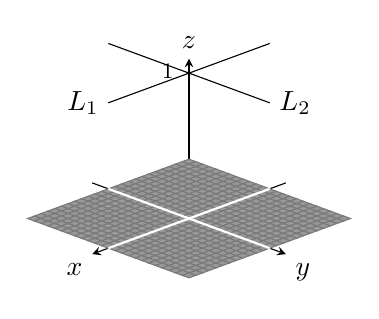
\begin{tikzpicture}
\begin{axis}[small,view/h=135,axis lines=center,colormap={}{gray(0.2cm)=(0.6);gray(1cm)=(0.9);},xlabel={$x$},ylabel={$y$},zlabel={$z$},enlargelimits=true,xtick={\empty},ytick={\empty},ztick={0,1},xlabel style={anchor={north east}},ylabel style={anchor={north west}},zlabel style={anchor={south}}]
\addplot3[surf,domain=-1:1,domain y=-1:1]{0};
\addplot3[thick,white,domain=-1:1](x,0,0);
\addplot3[thick,white,domain y=-1:1](0,y,0);
\addplot3[domain=-1:1](x,0,1)node[left]{$L_1$};
\addplot3[domain y=-1:1](0,y,1)node[right]{$L_2$};
\end{axis}
\end{tikzpicture}
\caption{تفاعل \عددی{f} چار کھلے ربعات اور لکیر \عددی{L_1}، \عددی{L_2} پر مشتمل ہے (مثال \حوالہ{مثال_کثیرالمتغیر_ٹکڑوں_میں_استمراری})۔}
\label{شکل_مثال_کثیرالمتغیر_ٹکڑوں_میں_استمراری}
\end{minipage}
\end{figure}
\جزوحصہء{استمرار اور جزوی تفرق کی موجودگی کا تعلق}
ایک نقطہ پر ایک تفاعل کا \عددی{x} اور \عددی{y} دونوں کے لحاظ سے جزوی تفرق موجود ہونے کے باوجود تفاعل غیر استمراری ہو سکتا ہے۔ یہ واحد متغیر  تفاعل سے مختلف ہے جہاں تفاعل کے تفرق کی موجودگی اس کی استمرار یقینی بناتی ہے۔ہاں (جیسا ہم اگلے حصہ میں دیکھیں گے)، اگر ایک قرص میں،  جس کا مرکز   \عددی{(x_0,y_0)} ہو،  \عددی{f(x,y)} کے جزوی تفرق موجود ہوں  جو پورے قرص میں استمراری ہوں تب \عددی{(x_0,y_0)} پر \عددی{f} استمراری ہو گا۔ 

\ابتدا{مثال}\شناخت{مثال_کثیرالمتغیر_ٹکڑوں_میں_استمراری}
درج ذیل تفاعل
\begin{align*}
f(x,y)=
\begin{cases}
0,&xy\ne 0\\
1,& xy=0
\end{cases}
\end{align*}
نقطہ \عددی{(0,0)} پر غیر استمراری ہے (شکل \حوالہ{شکل_مثال_کثیرالمتغیر_ٹکڑوں_میں_استمراری})۔ لکیر \عددی{y=x} پر چلتے ہوئے  نقطہ  \عددی{(x,y)} کا  \عددی{(x_0,y_0)} تک پہنچنے سے \عددی{f} کا حد \عددی{0} حاصل ہوتا ہے جبکہ \عددی{f(0,0)=1} ہے۔   نقطہ \عددی{(0,0)} پر \عددی{f} کے جزوی تفرقات \عددی{f_x}، \عددی{f_y}، جو شکل میں خط \عددی{L_1} اور \عددی{L_2} کی ڈھلوان ہیں،  دونوں موجود ہیں۔
\انتہا{مثال}
%===============

\جزوحصہء{دو رتبی جزوی  تفرقات}
تفاعل \عددی{f(x,y)} کو دو بار تفرق کرنے سے ہمیں  اس تفاعل کا دو رتبی تفرق ملتا ہے۔ان تفرقات کو عموماً درج ذیل سے ظاہر کیا جاتا ہے۔
\begin{align*}
\frac{\partial^{\,2}f}{\partial x^2}\quad \text{یا}\quad f_{xx}\\
\frac{\partial^{\,2}f}{\partial y^2}\quad \text{یا}\quad f_{yy}\\
\frac{\partial^{\,2}f}{\partial x \partial y}\quad \text{یا}\quad f_{yx}\\
\frac{\partial^{\,2}f}{\partial y \partial x}\quad \text{یا}\quad f_{xy}
\end{align*}
ان کی تعریفی مساوات درج ذیل ہیں
\begin{align*}
\frac{\partial^{\,2}f}{\partial x^2}=\frac{\partial}{\partial x}\big(\frac{\partial f}{\partial x}\big),\quad \frac{\partial^{\,2}f}{\partial x\partial y}=\frac{\partial}{\partial x}\big(\frac{\partial f}{\partial y}\big)
\end{align*}
جہاں تفرق لینے کی ترتیب  دھیان سے دیکھیں۔
\begin{align*}
\frac{\partial^{\,2}f}{\partial x\partial y}&=\frac{\partial}{\partial x}\big(\frac{\partial f}{\partial y}\big)&&\text{\RL{پہلے \عددی{y} اور بعد میں \عددی{x} کے ساتھ تفرق لیں}}\\
f_{yx}&=(f_y)_x&&\text{\RL{ان کا بھی یہی مطلب ہے۔}}
\end{align*}

\ابتدا{مثال}\شناخت{مثال_کثیرالمتغیر_مدغم_دو_رتبی}
اگر \عددی{f(x,y)=x\cos y+ye^x} ہو تب
\begin{align*}
\frac{\partial f}{\partial x}&=\cos y+ye^x\\
\frac{\partial^{\,2} f}{\partial y\partial x}&=\frac{\partial}{\partial y}\big(\frac{\partial f}{\partial x}\big)=-\sin y+e^x\\
\frac{\partial^{\,2} f}{\partial x^2}&=\frac{\partial}{\partial x}\big(\frac{\partial f}{\partial x}\big)=ye^x
\end{align*}
اور  درج ذیل ہوں گے۔
\begin{align*}
\frac{\partial f}{\partial y}&=-x\sin y+e^x\\
\frac{\partial^{\,2} f}{\partial x\partial y}&=\frac{\partial}{\partial x}\big(\frac{\partial f}{\partial y}\big)=-\sin y+e^x\\
\frac{\partial^{\,2} f}{\partial y^2}&=\frac{\partial}{\partial y}\big(\frac{\partial f}{\partial y}\big)=-x\cos y
\end{align*}
\انتہا{مثال}
%=================================

\جزوحصہء{مسئلہ یولر}
آپ نے مثال \حوالہ{مثال_کثیرالمتغیر_مدغم_دو_رتبی} میں دھیان دیا ہو گا کہ    مدغم      دو رتبی جزوی تفرقات
\begin{align*}
\frac{\partial^{\,2}f}{\partial y\partial x}\quad \text{}\quad \frac{\partial^{\,2}f}{\partial x\partial y}
\end{align*}
 کی قیمتیں ایک جیسی تھیں۔یہ محض اتفاق نہیں ہے۔جہاں  بھی \عددی{f}، \عددی{f_x}، \عددی{f_y}، \عددی{f_{xy}} اور \عددی{f_{yx}} استمراری ہوں یہ ایک دوسرے کے برابر ہوں گے۔

\ابتدا{مسئلہ}\شناخت{مسئلہ_کثیرالمتغیر_یولر}\موٹا{مدغم تفرق مسئلہ یا مسئلہ یولر}\\
اگر   ایک  کھلے  خطہ میں،  جس میں نقطہ \عددی{(a,b)} پایا جاتا ہو، \عددی{f(x,y)} اور اس کے جزوی تفرقات \عددی{f_x}، \عددی{f_y}، \عددی{f_{xy}} اور \عددی{f_{yx}} معین ہوں اور    \عددی{(a,b)}  پر یہ تمام  استمراری ہوں تب درج ذیل ہو گا۔
\begin{align}
f_{xy}(a,b)=f_{yx}(a,b)
\end{align} 
\انتہا{مسئلہ}
%================= 

مسئلہ یولر (مسئلہ \حوالہ{مسئلہ_کثیرالمتغیر_یولر}) کا ثبوت آپ کو  ضمیمہ \حوالہ{ضمیمہ_ط} میں ملے گا۔

مسئلہ \حوالہ{مسئلہ_کثیرالمتغیر_یولر} کہتا ہے کہ مدغم دو رتبی جزوی تفرق کے حصول میں ہم کسی بھی ترتیب سے تفرق لے سکتے ہیں۔ بعض اوقات ایسا مدد گار ثابت ہوتا ہے۔ 

\ابتدا{مثال}
درج ذیل تفاعل کے لئے \عددی{\tfrac{\partial^{\,2}w}{\partial x\partial y}} تلاش کریں۔
\begin{align*}
w=xy+\frac{e^y}{y^2+1}
\end{align*}
حل:\quad
ہمیں  \عددی{\tfrac{\partial^{\,2}w}{\partial x\partial y}} کہتا ہے کہ کہ پہلے \عددی{y} کے لحاظ سے تفرق لیں اور بعد میں \عددی{x} کے لحاظ سے تفرق لیں۔البتہ اگر ہم پہلے \عددی{x} اور بعد میں \عددی{y} کے لحاظ  سے تفرق لیں تب  نتیجہ زیادہ جلدی   اور زیادہ  آسانی سے صرف دو  قدموں  میں   حاصل ہوتا ہے۔ 
\begin{align*}
\frac{\partial w}{\partial x}&=y\\
\frac{\partial^{\,2}w}{\partial y\partial x}&=1
\end{align*}
اب  پہلے \عددی{y} اور بعد میں \عددی{x} کا تفرق لیتے ہوئے اسی کو دوبارہ حل کر کے دیکھیں۔
\انتہا{مثال}
%=================

\جزوحصہء{مزید بلند رتبہ کے جزوی تفرقات}
عملی استعمال میں یک رتبی اور دو رتبی جزوی تفرقات   زیادہ کثرت سے پائے جاتے ہیں لہٰذا ہمیں عموماً انہیں سے واسطہ ہو گا ۔جہاں تک تفاعل کے بلند تفرقات  کی بات ہے، ہم ایک تفاعل کا تفرق  جتنی بار چاہیں لیں سکتے ہیں بشرطیکہ ایسے تفرقات موجود ہوں۔ یوں ہم تین رتبی اور چار رتبی تفرقات لے سکتے ہیں جنہیں درج ذیل علامتوں  کی طرز    پر  ظاہر کیا جائے گا۔
 \begin{align*}
\frac{\partial^{\,3}f}{\partial x\partial^{\,2}y}&=f_{yyx}\\
\frac{\partial^{\,4}f}{\partial^{\,2}x\partial^{\,2}y}&=f_{yyxx}
\end{align*}
دو رتبی تفرق کی طرح،   تفرق کی ترتیب غیر اہم ہے جب تک تمام  تفرقات استمراری ہوں۔


\جزوحصہء{سوالات}
\ابتدا{سوالات}
\موٹا{یک رتبی جزوی تفرق کی تلاش}\\
سوال \حوالہ{ سوال_کثیرالمتغیر_یک_رتبی_جزوی_الف}  تا سوال  \حوالہ{سوال_کثیرالمتغیر_یک_رتبی_جزوی_ب} میں \عددی{\tfrac{\partial f}{\partial x}} اور \عددی{\tfrac{\partial f}{\partial y}} تلاش کریں۔

\ابتدا{سوال}\شناخت{ سوال_کثیرالمتغیر_یک_رتبی_جزوی_الف}
$f(x,y)=2x^2-3y-4$
\انتہا{سوال}  
   %======== 
  \ابتدا{جواب}
\wf{\unexpanded{
$\tfrac{\partial f}{\partial x}=4x,\quad \tfrac{\partial f}{\partial y}=-3$
}}
\انتہا{جواب}
%===================
\ابتدا{سوال}
$f(x,y)=x^2-xy+y^2$
\انتہا{سوال}
%====================
\ابتدا{سوال}
$f(x,y)=(x^2-1)(y+2)$
\انتہا{سوال}  
   %======== 
  \ابتدا{جواب}
\wf{\unexpanded{
$\tfrac{\partial f}{\partial x}=2x(y+2),\quad \tfrac{\partial f}{\partial y}=x^2-1$
}}
\انتہا{جواب}
%====================
\ابتدا{سوال}
$f(x,y)=5xy-7x^2-y^2+3x-6y+2$
\انتہا{سوال}
%====================
\ابتدا{سوال}
$f(x,y)=(xy-1)^2$
\انتہا{سوال}  
   %======== 
  \ابتدا{جواب}
\wf{\unexpanded{
$\tfrac{\partial f}{\partial x}=2y(xy-1),\quad \tfrac{\partial f}{\partial y}=2x(xy-1)$
}}
\انتہا{جواب}
%====================
\ابتدا{سوال}
$f(x,y)=(2x-3y)^3$
\انتہا{سوال}
%====================
\ابتدا{سوال}
$f(x,y)=\sqrt{x^2+y^2}$
\انتہا{سوال}  
   %======== 
  \ابتدا{جواب}
\wf{\unexpanded{
$\tfrac{\partial f}{\partial x}=\tfrac{x}{\sqrt{x^2+y^2}},\quad \tfrac{\partial f}{\partial y}=\tfrac{y}{\sqrt{x^2+y^2}}$
}}
\انتہا{جواب}
%====================
\ابتدا{سوال}
$f(x,y)=(x^3+y/2)^{2/3}$
\انتہا{سوال}
%====================
\ابتدا{سوال}
$f(x,y)=\frac{1}{x+y}$
\انتہا{سوال}  
   %======== 
  \ابتدا{جواب}
\wf{\unexpanded{
$\tfrac{\partial f}{\partial x}=\tfrac{-1}{(x+y)^2},\quad \tfrac{\partial f}{\partial y}=\tfrac{-1}{(x+y)^2}$
}}
\انتہا{جواب}
%====================
\ابتدا{سوال}
$f(x,y)=\frac{x}{x^2+y^2}$
\انتہا{سوال}
%====================
\ابتدا{سوال}
$f(x,y)=\frac{x+y}{xy-1}$
\انتہا{سوال}  
   %======== 
  \ابتدا{جواب}
\wf{\unexpanded{
$\tfrac{\partial f}{\partial x}=\tfrac{-y^2-1}{(xy-1)^2},\quad \tfrac{\partial f}{\partial y}=\tfrac{-x^2-1}{(xy-1)^2}$
}}
\انتہا{جواب}
%====================
\ابتدا{سوال}
$f(x,y)=\tan^{-1}\frac{y}{x}$
\انتہا{سوال}
%====================
\ابتدا{سوال}
$f(x,y)=e^{x+y+1}$
\انتہا{سوال}  
   %======== 
  \ابتدا{جواب}
\wf{\unexpanded{
$\tfrac{\partial f}{\partial x}=e^{x+y+1},\quad \tfrac{\partial f}{\partial y}=e^{x+y+1}$
}}
\انتہا{جواب}
%====================
\ابتدا{سوال}
$f(x,y)=e^{-x}\sin(x+y)$
\انتہا{سوال}
%====================
\ابتدا{سوال}
$f(x,y)=\ln(x+y)$
\انتہا{سوال}  
   %======== 
  \ابتدا{جواب}
\wf{\unexpanded{
$\tfrac{\partial f}{\partial x}=\tfrac{1}{x+y},\quad \tfrac{\partial f}{\partial y}=\tfrac{1}{x+y}$
}}
\انتہا{جواب}
%====================
\ابتدا{سوال}
$f(x,y)=e^{xy}\ln y$
\انتہا{سوال}
%====================
\ابتدا{سوال}
$f(x,y)=\sin^2(x-3y)$
\انتہا{سوال}  
   %======== 
  \ابتدا{جواب}
\wf{\unexpanded{
$\tfrac{\partial f}{\partial x}=2\sin(x-3y)\cos(x-3y),$\\
$\tfrac{\partial f}{\partial y}=-6\sin(x-3y)\cos(x-3y)$
}}
\انتہا{جواب}
%====================
\ابتدا{سوال}
$f(x,y)=\cos^2(3x-y^2)$
\انتہا{سوال}
%====================
\ابتدا{سوال}
$f(x,y)=x^y$
\انتہا{سوال}  
   %======== 
  \ابتدا{جواب}
\wf{\unexpanded{
$\tfrac{\partial f}{\partial x}=yx^{y-1},\quad \tfrac{\partial f}{\partial y}=x^y\ln x$
}}
\انتہا{جواب}
%====================
\ابتدا{سوال}
$f(x,y)=\log_y x$
\انتہا{سوال}
%====================
\ابتدا{سوال}
$f(x,y)=\int_x^yg(t)\dif t\quad \text{\RL{تمام \عددی{t} کے لئے \عددی{g} استمراری ہے}}$
\انتہا{سوال}  
   %======== 
  \ابتدا{جواب}
\wf{\unexpanded{
$\tfrac{\partial f}{\partial x}=-g(x),\quad \tfrac{\partial f}{\partial y}=g(y)$
}}
\انتہا{جواب}
%====================
\ابتدا{سوال}\شناخت{سوال_کثیرالمتغیر_یک_رتبی_جزوی_ب}
$f(x,y)=\sum\limits_{n=0}^{\infty}(xy)^n\quad (\abs{xy}<1)$
\انتہا{سوال}
%====================

سوال \حوالہ{سوال_کثیرالمتغیر_یک_رتبی_تین_متغیر_تفاعل_الف} تا سوال \حوالہ{سوال_کثیرالمتغیر_یک_رتبی_تین_متغیر_تفاعل_ب} میں \عددی{f_x}، \عددی{f_y}  اور \عددی{f_z} تلاش کریں۔

\ابتدا{سوال}\شناخت{سوال_کثیرالمتغیر_یک_رتبی_تین_متغیر_تفاعل_الف}
$f(x,y,z)=1+xy^2-2z^2$
\انتہا{سوال}  
   %======== 
  \ابتدا{جواب}
\wf{\unexpanded{
$f_x=y^2,\quad f_y=2xy,\quad f_z=-4z$
}}
\انتہا{جواب}
%===================
\ابتدا{سوال}
$f(x,y,z)=xy+yz+xz$
\انتہا{سوال}
%=====================
\ابتدا{سوال}
$f(x,y,z)=x-\sqrt{y^2+z^2}$
\انتہا{سوال}  
   %======== 
  \ابتدا{جواب}
\wf{\unexpanded{
$f_x=1,f_y=-y(y^2+z^2)^{-1/2},$\\
$f_z=-z(y^2+z^2)^{-1/2}$
}}
\انتہا{جواب}
%=====================
\ابتدا{سوال}
$f(x,y,z)=(x^2+y^2+z^2)^{-1/2}$
\انتہا{سوال}
%=====================
\ابتدا{سوال}
$f(x,y,z)=\sin^{-1}(xyz)$
\انتہا{سوال}  
   %======== 
  \ابتدا{جواب}
\wf{\unexpanded{
$f_x=\tfrac{yz}{\sqrt{1-x^2y^2z^2}}, f_y=\tfrac{xz}{\sqrt{1-x^2y^2z^2}},$\\
$f_z=\tfrac{xy}{\sqrt{1-x^2y^2z^2}}$
}}
\انتہا{جواب}
%=====================
\ابتدا{سوال}
$f(x,y,z)=\sec^{-1}(x+yz)$
\انتہا{سوال}
%=====================
\ابتدا{سوال}
$f(x,y,z)=\ln(x+2y+3z)$
\انتہا{سوال}  
   %======== 
  \ابتدا{جواب}
\wf{\unexpanded{
$f_x=\tfrac{1}{x+2y+3z},f_y=\tfrac{2}{x+2y+3z},$\\
$f_z=\tfrac{3}{x+2y+3z}$
}}
\انتہا{جواب}
%=====================
\ابتدا{سوال}
$f(x,y,z)=yz\ln(xy)$
\انتہا{سوال}
%=====================
\ابتدا{سوال}
$f(x,y,z)=e^{-(x^2+y^2+z^2)}$
\انتہا{سوال}  
   %======== 
  \ابتدا{جواب}
\wf{\unexpanded{
$f_x=-2xe^{-(x^2+y^2+z^2)},$\\
$f_y=-2ye^{-(x^2+y^2+z^2)},$\\
$f_z=-2ze^{-(x^2+y^2+z^2)}$
}}
\انتہا{جواب}
%=====================
\ابتدا{سوال}
$f(x,y,z)=e^{-xyz}$
\انتہا{سوال}
%=====================
\ابتدا{سوال}
$f(x,y,z)=\tanh(x+2y+3z)$
\انتہا{سوال}  
   %======== 
  \ابتدا{جواب}
\wf{\unexpanded{
$f_x=\sech^2(x+2y+3z),$\\
$f_y=2\sech^2(x+2y+3z),$\\
$f_z=3\sech^2(x+2y+3z)$
}}
\انتہا{جواب}
%=====================
\ابتدا{سوال}\شناخت{سوال_کثیرالمتغیر_یک_رتبی_تین_متغیر_تفاعل_ب}
$f(x,y,z)=\sinh(xy-z^2)$
\انتہا{سوال}
%=====================

سوال \حوالہ{سوال_کثیر_المتغیر_ہر_متغیر_جزوی_الف} تا سوال \حوالہ{سوال_کثیر_المتغیر_ہر_متغیر_جزوی_ب} میں ہر متغیر کے لحاظ سے تفاعل کا جزوی تفرق تلاش کریں۔

\ابتدا{سوال}\شناخت{سوال_کثیر_المتغیر_ہر_متغیر_جزوی_الف}
$f(t,\alpha)=\cos(2\pi t-\alpha)$
\انتہا{سوال}  
   %======== 
  \ابتدا{جواب}
\wf{\unexpanded{
$\tfrac{\partial f}{\partial t}=-2\pi\sin(2\pi t-\alpha),$\\
$\tfrac{\partial f}{\partial \alpha}=\sin(2\pi t-\alpha)$
}}
\انتہا{جواب}
%=================
\ابتدا{سوال}
$g(u,v)=v^2e^{2u/v}$
\انتہا{سوال}
%=================
\ابتدا{سوال}
$h(\rho,\theta,\phi)=\rho\sin\theta\cos\phi$
\انتہا{سوال}  
   %======== 
  \ابتدا{جواب}
\wf{\unexpanded{
$\tfrac{\partial h}{\partial \rho}=\sin\theta\cos\phi,$\\
$\tfrac{\partial h}{\partial \theta}=\rho\cos\theta\cos\phi,$\\
$\frac{\partial h}{\partial \phi}=-\rho\sin\theta\sin\phi$
}}
\انتہا{جواب}
%=================
\ابتدا{سوال}
$g(r,\theta,z)=r(1-\cos\theta)-z$
\انتہا{سوال}
%=================
\ابتدا{سوال}\ترچھا{قلب کا کام}\\
$W(P,H,\delta,v,g)=PH+\frac{H\delta v^2}{2g}$
\انتہا{سوال}  
   %======== 
  \ابتدا{جواب}
\wf{\unexpanded{
$W_P(P,H,\delta,v,g)=H,$\\
$W_H(P,H,\delta,v,g)=P+\tfrac{\delta v^2}{2g},$\\
$W_{\delta}(P,H,\delta,v,g)=\tfrac{Hv^2}{2g},$\\
$W_v(P,H,\delta,v,g)=\tfrac{H\delta v}{g},$\\
$W_g(P,H,\delta,v,g)=-\tfrac{H\delta v^2}{2g^2}$
}}
\انتہا{جواب}
%=================
\ابتدا{سوال}\شناخت{سوال_کثیر_المتغیر_ہر_متغیر_جزوی_ب}
$A(c,h,k,m,q)=\frac{km}{q}+cm+\frac{hq}{2}$
\انتہا{سوال}
%=================

\موٹا{دو رتبی جزوی تفرق کا حصول}\\
سوال \حوالہ{سوال_کثیرالمتغیر_تمام_جزوی_تلاش_الف} تا سوال \حوالہ{سوال_کثیرالمتغیر_تمام_جزوی_تلاش_ب} میں تفاعل کے تمام دو رتبی جزوی تفرقات تلاش کریں۔

\ابتدا{سوال}\شناخت{سوال_کثیرالمتغیر_تمام_جزوی_تلاش_الف}
$f(x,y)=x+y+xy$
\انتہا{سوال}  
   %======== 
  \ابتدا{جواب}
\wf{\unexpanded{
$\tfrac{\partial f}{\partial x}=1+y, \tfrac{\partial f}{\partial y}=1+x,\frac{\partial^{\,2} f}{\partial x^2}=0,$\\
$\frac{\partial^{\,2} f}{\partial y^2}=0,\frac{\partial^{\,2} f}{\partial y\partial x}=\frac{\partial^{\,2} f}{\partial x\partial y}=1$
}}
\انتہا{جواب}
%=================
\ابتدا{سوال}
$f(x,y)=\sin xy$
\انتہا{سوال}
%=================
\ابتدا{سوال}
$g(x,y)=x^2y+\cos y+y\sin x$
\انتہا{سوال}  
   %======== 
  \ابتدا{جواب}
\wf{\unexpanded{
$\tfrac{\partial g}{\partial x}=2xy+y\cos x,$\\
$\tfrac{\partial g}{\partial y}=x^2-\sin y+\sin x,$\\
$\frac{\partial^{\,2} g}{\partial x^2}=2y-y\sin x,\frac{\partial^{\,2} g}{\partial y^2}=-\cos y,$\\
$\frac{\partial^{\,2} g}{\partial y\partial x}=\frac{\partial^{\,2} f}{\partial x\partial y}=2x+\cos x$
}}
\انتہا{جواب}
%=================
\ابتدا{سوال}
$h(x,y)=xe^y+y+1$
\انتہا{سوال}
%=================
\ابتدا{سوال}
$r(x,y)=\ln(x,y)$
\انتہا{سوال}  
   %======== 
  \ابتدا{جواب}
\wf{\unexpanded{
$\tfrac{\partial r}{\partial x}=\tfrac{1}{x+y},\tfrac{\partial r}{\partial y}=\tfrac{1}{x+y},\frac{\partial^{\,2} r}{\partial x^2}=\tfrac{-1}{(x+y)^2}$\\
$\frac{\partial^{\,2} r}{\partial y^2}=\tfrac{-1}{(x+y)^2},\frac{\partial^{\,2} r}{\partial y\partial x}=\frac{\partial^{\,2} f}{\partial x\partial y}=\tfrac{-1}{(x+y)^2}$
}}
\انتہا{جواب}
%=================
\ابتدا{سوال}\شناخت{سوال_کثیرالمتغیر_تمام_جزوی_تلاش_ب}
$s(x,y)=\tan^{-1}\frac{y}{x}$
\انتہا{سوال}
%=================

\موٹا{مدغم جزوی تفرقات}\\
سوال \حوالہ{سوال_کثیرالمتغیر_تصدیق_مدغم_الف} تا سوال \حوالہ{سوال_کثیرالمتغیر_تصدیق_مدغم_ب}   میں \عددی{w_{xy}=w_{yx}} کی   تصدیق کریں۔

\ابتدا{سوال}\شناخت{سوال_کثیرالمتغیر_تصدیق_مدغم_الف}
$w=\ln(2x+3y)$
\انتہا{سوال}  
   %======== 
  \ابتدا{جواب}
\wf{\unexpanded{
$\tfrac{\partial w}{\partial x}=\tfrac{2}{2x+3y},\tfrac{\partial w}{\partial y}=\tfrac{3}{2x+3y},$\\
$\frac{\partial^{\,2} w}{\partial y\partial x}=\frac{\partial^{\,2} f}{\partial x\partial y}=\tfrac{-6}{(2x+3y)^2}$
}}
\انتہا{جواب}
%===============
\ابتدا{سوال}
$w=e^x+x\ln y+y\ln x$
\انتہا{سوال}
%==================
\ابتدا{سوال}
$w=xy^2+x^2y^3+x^3y^4$
\انتہا{سوال}  
   %======== 
  \ابتدا{جواب}
\wf{\unexpanded{
$\tfrac{\partial w}{\partial x}=y^2+2xy^3+3x^2y^4,$\\
$\tfrac{\partial w}{\partial y}=2xy+3x^2y^2+4x^3y^3,$\\
$\frac{\partial^{\,2} w}{\partial y\partial x}=2y+6xy^2+12x^2y^3,$\\
$\frac{\partial^{\,2} f}{\partial x\partial y}=2y+6xy^2+12x^2y^3$
}}
\انتہا{جواب}
%==================
\ابتدا{سوال}\شناخت{سوال_کثیرالمتغیر_تصدیق_مدغم_ب}
$w=x\sin y+y\sin x+xy$
\انتہا{سوال}
%==================
\ابتدا{سوال}
بغیر قلم اٹھائے   بتائیں کہ درج ذیل میں \عددی{x} کے لحاظ سے پہلے اور \عددی{y} کے  لحاظ سے بعد میں یا اس کے الٹ حل کرتے ہوئے  \عددی{f_{xy}} زیادہ جلدی حاصل ہو گا۔
\begin{enumerate}[a.]
\item
$f(x,y)=x\sin y+e^y$
\item
$f(x,y)=\frac{1}{x}$
\item
$f(x,y)=y+\frac{x}{y}$
\item
$f(x,y)=y+x^2y+4y^3-\ln(y^2+1)$
\item
$f(x,y)=x^2+5xy+\sin x+7e^x$
\item
$f(x,y)=x\ln xy$
\end{enumerate}
\انتہا{سوال}  
   %======== 
  \ابتدا{جواب}
\wf{\unexpanded{
(ا) پہلے \عددی{x}، (ب) پہلے \عددی{y}، (ج) پہلے \عددی{x}، (د) پہلے \عددی{x}، (ہ) پہلے \عددی{y}، (ہ) پہلے \عددی{y} 
}}
\انتہا{جواب}
%===============
\ابتدا{سوال}
درج ذیل میں تمام کا پانچ رتبی جزوی تفرق \عددی{\tfrac{\partial^{\,5}f}{\partial x^2\partial y^3}} صفر کے برابر ہے۔ اس کی تصدیق کرنے کی خاطر آپ کس متغیر کے لحاظ سے پہلے جزوی تفرق لیں گے؟ بغیر کچھ لکھے جواب دینے کی کوشش کریں۔
\begin{enumerate}[a.]
\item
$f(x,y)=y^2x^4e^x+2$
\item
$f(x,y)=y^2+y(\sin x-x^4)$
\item
$f(x,y)=x^2+5xy+\sin x+7e^x$
\item
$f(x,y)=xe^{y^2/2}$
\end{enumerate}
\انتہا{سوال}
%==============

\موٹا{جزوی تفرق کی تعریف کا استعمال}\\
سوال \حوالہ{سوال_کثیرالمتغیر_تعریف_حد_جزوی_تفرق_الف} اور سوال \حوالہ{سوال_کثیرالمتغیر_تعریف_حد_جزوی_تفرق_ب} میں جزوی تفرق کی تعریف بذریعہ حد استعمال کرتے ہوئے دیے گئے نقطہ پر تفاعل کا جزوی تفرق حاصل کریں۔

\ابتدا{سوال}\شناخت{سوال_کثیرالمتغیر_تعریف_حد_جزوی_تفرق_الف}
$f(x,y)=1-x+y-3x^2y,\quad \frac{\partial f}{\partial x},\,\frac{\partial f}{\partial y},\quad (1,2)$
\انتہا{سوال}  
   %======== 
  \ابتدا{جواب}
\wf{\unexpanded{
$f_x(1,2)=-13, f_y(1,2)=-2$
}}
\انتہا{جواب}
%==================
\ابتدا{سوال}\شناخت{سوال_کثیرالمتغیر_تعریف_حد_جزوی_تفرق_ب}
$f(x,y)=4+2x-3y-xy^2,\quad \frac{\partial f}{\partial x},\,\frac{\partial f}{\partial y},\quad (-2,1)$
\انتہا{سوال}
%=================
\ابتدا{سوال}
فرض کریں \عددی{w=f(x,y,z)} تین غیر تابع متغیرات کا تفاعل ہے۔ نقطہ \عددی{(x_0,y_0,z_0)} پر جزوی تفرق  \عددی{\tfrac{\partial f}{\partial z}} کی باضابطہ تعریف  لکھیں کریں۔ اس تعریف کو استعمال کرتے ہوئے \عددی{(1,2,3)} پر \عددی{f(x,y,z)=x^2yz^2} کا \عددی{\tfrac{\partial f}{\partial z}} تلاش کریں۔
\انتہا{سوال}  
   %======== 
  \ابتدا{جواب}
\wf{\unexpanded{
$12$
}}
\انتہا{جواب}
%===================
\ابتدا{سوال}
فرض کریں \عددی{w=f(x,y,z)} تین غیر تابع متغیرات کا تفاعل ہے۔ نقطہ \عددی{(x_0,y_0,z_0)} پر جزوی تفرق  \عددی{\tfrac{\partial f}{\partial y}} کی باضابطہ تعریف  لکھیں کریں۔ اس تعریف کو استعمال کرتے ہوئے \عددی{(-1,0,3)} پر \عددی{f(x,y,z)=-2xy^2+yz^2} کا \عددی{\tfrac{\partial f}{\partial z}} تلاش کریں۔
\انتہا{سوال}
%===============
\موٹا{خفی جزوی تفرقات}\\
\ابتدا{سوال}
 ذیل مساوات  میں     غیر تابع متغیرات \عددی{x} اور \عددی{y} کا تفاعل \عددی{z} پیش کیا گیا ہے۔ نقطہ \عددی{(1,1,1)} پر \عددی{\tfrac{\partial z}{\partial x}} کی قیمت تلاش کریں۔ اس نقطہ پر   یہ  جزوی تفرق  موجود ہے۔  
\begin{align*}
xy+z^3x-2yz=0
\end{align*}
\انتہا{سوال}  
   %======== 
  \ابتدا{جواب}
\wf{\unexpanded{
$-2$
}}
\انتہا{جواب}
%====================
\ابتدا{سوال}
 ذیل مساوات  میں     غیر تابع متغیرات \عددی{x} اور \عددی{y} کا تفاعل \عددی{z} پیش کیا گیا ہے۔ نقطہ \عددی{(1,-1,-3)} پر \عددی{\tfrac{\partial z}{\partial x}} کی قیمت تلاش کریں۔ اس نقطہ پر   یہ  جزوی تفرق  موجود ہے۔  
\begin{align*}
xz+y\ln x-x^2+4=0
\end{align*}
\انتہا{سوال}
%===================
سوال \حوالہ{سوال_کثیرالمتغیر_مثلث_الف} اور سوال \حوالہ{سوال_کثیرالمتغیر_مثلث_الف} درج ذیل مثلث  کے بارے میں ہے۔
\begin{center}
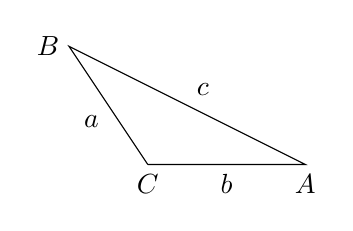
\begin{tikzpicture}
\draw(0,0)node[below]{$C$}--(2,0)node[below]{$A$}node[pos=0.5,below]{$b$}--(-1,1.5)node[left]{$B$}node[pos=0.5,above right]{$c$}--(0,0)node[pos=0.5,below left]{$a$};
\end{tikzpicture}
\end{center}

\ابتدا{سوال}\شناخت{سوال_کثیرالمتغیر_مثلث_الف}
\عددی{A} کو خفی طور پر \عددی{a}، \عددی{b} اور \عددی{c} کا تفاعل لکھ کر \عددی{\tfrac{\partial A}{\partial a}} اور \عددی{\tfrac{\partial A}{\partial b}} تلاش کریں۔
\انتہا{سوال}  
   %======== 
  \ابتدا{جواب}
\wf{\unexpanded{
$\tfrac{\partial A}{\partial a}=\tfrac{a}{bc\sin A},\tfrac{\partial A}{\partial b}=\tfrac{c\cos A-b}{bc\sin A}$
}}
\انتہا{جواب}
%=================
\ابتدا{سوال}\شناخت{سوال_کثیرالمتغیر_مثلث_ب}
\عددی{a} کو خفی طور پر \عددی{A}، \عددی{b} اور \عددی{B} کا تفاعل لکھ کر \عددی{\tfrac{\partial a}{\partial A}} اور \عددی{\tfrac{\partial a}{\partial B}} تلاش کریں۔
\انتہا{سوال}
%=================
\ابتدا{سوال}\شناخت{سوال_کثیرالمتغیر_پیچیدہ_مساوات}
غیر تابع متغیرات \عددی{x} اور \عددی{y} کی صورت میں تفاعل  \عددی{u} اور \عددی{v} مساوات \عددی{x=v\ln u} اور \عددی{y=u\ln v} دیتی ہیں۔ جزوی تفرق \عددی{v_x} ،  جو موجود ہے، کو \عددی{u} اور \عددی{v} کی صورت میں لکھیں۔ (اشارہ: دونوں مساوات کا تفرق  \عددی{x} ا کے لحاظ سے لے کر \عددی{v_x} کے لئے حل کریں۔)
\انتہا{سوال}  
   %======== 
  \ابتدا{جواب}
\wf{\unexpanded{
$v_x=\tfrac{\ln v}{(\ln u)(\ln v)-1}$
}}
\انتہا{جواب}
%=====================
\ابتدا{سوال}
غیر تابع متغیرات \عددی{u} اور \عددی{v} کی صورت میں تفاعل  \عددی{x} اور \عددی{y} مساوات \عددی{u=x^2-y^2} اور \عددی{v=x^2-y} دیتی ہیں۔ جزوی تفرق \عددی{\tfrac{\partial x}{\partial u}} اور  \عددی{\tfrac{\partial y}{\partial u}} ،  جو موجود  ہیں تلاش کریں۔ (اشارہ:سوال \حوالہ{سوال_کثیرالمتغیر_پیچیدہ_مساوات} میں دیا گیا اشارہ دیکھیں۔)   اب \عددی{s=x^2+y} لیتے ہوئے \عددی{\tfrac{\partial s}{\partial u}} حاصل کریں۔
\انتہا{سوال}
%=====================
\موٹا{مساوات لاپلاس}\\
\ترچھا{تین بعدی مساوات لاپلاس}
\begin{align}\label{مساوات_کثیر_المتغیر_مساوات_لاپلاس_الف}
\frac{\partial^{\,2}f}{\partial x^2}+\frac{\partial^{\,2}f}{\partial y^2}+\frac{\partial^{\,2}f}{\partial z^2}=0
\end{align}
کو فضا میں  برقرار حال حراری تقسیم \عددی{T=f(x,y,z)}، تجاذبی  مخفی قوہ اور برقی ساکن مخفی قوہ   مطمئن کرتے ہیں۔ مساوات \حوالہ{مساوات_کثیر_المتغیر_مساوات_لاپلاس_الف} سے جزو \عددی{\tfrac{\partial f}{\partial z}} نکالنے سے    \ترچھا{دو بعدی مساوات لاپلاس}
 \begin{align}\label{مساوات_کثیر_المتغیر_مساوات_لاپلاس_ب}
\frac{\partial^{\,2}f}{\partial x^2}+\frac{\partial^{\,2}f}{\partial y^2}=0
\end{align}
حاصل ہوتی ہے جو مستوی میں  خفی قوہ اور برقرار حال حراری تقسیم  بیان کرتی ہے (شکل \حوالہ{شکل_کثیر_المتغیر_لاپلاس_اور_حرارت})۔

دکھائیں کہ سوال \حوالہ{سوال_کثیرالمتغیر_مطمئن_لاپلاس_الف} تا سوال \حوالہ{سوال_کثیرالمتغیر_مطمئن_لاپلاس_ب} میں  دیا ہر ایک  تفاعل مساوات لاپلاس میں سے کسی ایک کو مطمئن کرتا ہے۔ 

\ابتدا{سوال}\شناخت{سوال_کثیرالمتغیر_مطمئن_لاپلاس_الف}
$f(x,y,z)=x^2+y^2-2z^2$
\انتہا{سوال}
%==============
\ابتدا{سوال}
$f(x,y,z)=2z^3-3(x^2+y^2)z$
\انتہا{سوال}
%=====================
\ابتدا{سوال}
$f(x,y)=e^{-2y}\cos 2x$
\انتہا{سوال}
%=====================
\ابتدا{سوال}
$f(x,y)=\ln\sqrt{x^2+y^2}$
\انتہا{سوال}
%=====================
\ابتدا{سوال}
$f(x,y,z)=(x^2+y^2+z^2)^{-1/2}$
\انتہا{سوال}
%=====================
\ابتدا{سوال}\شناخت{سوال_کثیرالمتغیر_مطمئن_لاپلاس_ب}
$f(x,y,z)=e^{2x+4y}\cos 5z$
\انتہا{سوال}
%=====================
\begin{figure}
\centering
\begin{subfigure}{0.45\textwidth}
\centering
\begin{tikzpicture}[font=\small]
\pgfmathsetmacro{\a}{2.5}
\pgfmathsetmacro{\b}{1.25}
\pgfmathsetmacro{\t}{0.1}
\pgfmathsetmacro{\ang}{45}
\draw[fill=llgray](0,0)coordinate(aa)--++(\a,0)coordinate(bb)--++(\ang:\b)coordinate(cc)--++(-\a,0)coordinate(dd)--(0,0);
\draw(0,0)--++(0,-\t)coordinate(aaa)--++(\a,0)coordinate(bbb)--++(\ang:\b)coordinate(ccc)--(cc);
\draw[fill=llgray](aa)--(aaa)--(bbb)--(ccc)--(cc)--(bb)--(aa);
\draw(bb)--(bbb);
\draw(\a/2,-0.8) circle (0.3cm and 0.1cm);
\draw(\a/2-0.3,-0.8)--++(0,-0.5);
\draw(\a/2+0.3,-0.8)--++(0,-0.5);
\draw[fill=white](\a/2,-0.3)to [out=-135,in=110]++(0,-0.5) to [out=80,in=-45]++(0,0.5);
\draw(3/4*\a,\b/2)node[circ]{}node[pin=60:{$\frac{\partial^{\,2}f}{\partial x^2}+\frac{\partial^{\,2}f}{\partial y^2}=0$}]{};
\end{tikzpicture}
\caption{}
\end{subfigure}\hfill
\begin{subfigure}{0.45\textwidth}
\centering
\begin{tikzpicture}[font=\small]
\pgfmathsetmacro{\a}{2.5}
\pgfmathsetmacro{\b}{1.25}
\pgfmathsetmacro{\c}{0.6}
\pgfmathsetmacro{\t}{0.1}
\pgfmathsetmacro{\ang}{45}
\draw(0,0)coordinate(aa)--++(\a,0)coordinate(bb)--++(\ang:\b)coordinate(cc)--++(-\a,0)coordinate(dd)--++(\ang:-\b);
\draw(0,\c)coordinate(taa)--++(\a,0)coordinate(tbb)--++(\ang:\b)coordinate(tcc)--++(-\a,0)coordinate(tdd)--++(\ang:-\b);
\draw[fill=llgray,opacity=0.5](0,\c/2)coordinate(maa)--++(\a,0)coordinate(mbb)--++(\ang:\b)coordinate(mcc)--++(-\a,0)coordinate(mdd)--++(\ang:-\b);
\draw[dashed](0,\c/2-\t)--++(\ang:\b)--++(\a,0);
\draw[fill=llgray,opacity=0.5](0,\c/2-\t)--++(\a,0)--++(\ang:\b)--++(0,\t)--++(\ang:-\b)--++(-\a,0)--++(0,-\t);
\draw(aa)--(taa)  (bb)--(tbb)  (cc)--(tcc)  (dd)--(tdd);
\draw(1/2*\a,\b/2+\t)node[circ]{}node[pin={[pin distance=1cm]70:{$\frac{\partial^{\,2}f}{\partial x^2}+\frac{\partial^{\,2}f}{\partial y^2}+\frac{\partial^{\,2}f}{\partial z^2}=0$}}]{};
\end{tikzpicture}
\caption{مستوی کی سرحدی (کناروں کی) حرارت قابو کی گئی ہے۔}
\end{subfigure}
\caption{مستوی اور ٹھوس اجسام میں برقرار حال حرارت، مساوات لاپلاس کو مطمئن کرتی ہے۔}
\label{شکل_کثیر_المتغیر_لاپلاس_اور_حرارت}
\end{figure}

\موٹا{مساوات موج}\\
سمندر  کے کنارے کھڑے  ہو کر سمندری امواج کی لی گئی  تصویر  میں نشیب و فراز کا   ایک منظم نقش نظر آتا ہے۔ہمیں  فضا میں  فاصلہ کے لحاظ سے   دوری انتصابی حرکت نظر آتی ہے۔ پانی میں کھڑے ہو کر ہم گزرتی امواج کی بنا پانی کا اتار چھڑاو محسوس کرتے ہیں۔ ہم وقت کے لحاظ سے دوری انتصابی حرکت  دیکھتے ہیں۔طبیعیات  میں اس خوبصورت   تشاکلی کو \ترچھا{یک بعدی مساوات موج}
\begin{align}
\frac{\partial^{\,2}u}{\partial t^2}=c^2\frac{\partial ^{\,2}w}{\partial x^2}
\end{align}
بیان کرتی ہے جہاں  قد موج  \عددی{w}، فاصلاتی متغیر  \عددی{x}، لمحاتی متغیر \عددی{t} اور موج کی رفتار  \عددی{c}  ہے۔ 

سمندری سطح پر فاصلہ \عددی{x} ہو گا لیکن دیگر عملی استعمال میں \عددی{x}  ارتعاش پذیر  تار کے ساتھ ساتھ  فاصلہ، ہوا میں فاصلہ (صوتی امواج)، یا فضا میں فاصلہ  (امواج نور)  ہو سکتا ہے۔  عدد \عددی{c} کی قیمت موج کی قسم اور  ذریعہ پر منحصر ہو  گا۔

دکھائیں کہ سوال \حوالہ{سوال_کثیرالمتغیر_مساوات_موج_الف} تا سوال \حوالہ{سوال_کثیرالمتغیر_مساوات_موج_ب}  میں تمام  تفاعل مساوات موج کو مطمئن کرتے ہیں۔ 

\ابتدا{سوال}\شناخت{سوال_کثیرالمتغیر_مساوات_موج_الف}
$w=\sin(x+ct)$
\انتہا{سوال}
%===================
\ابتدا{سوال}
$w=\cos(2x+2ct)$
\انتہا{سوال}
%==================
\ابتدا{سوال}
$w=\sin(x+ct)+\cos(2x+2ct)$
\انتہا{سوال}
%==================
\ابتدا{سوال}
$w=\ln(2x+2ct)$
\انتہا{سوال}
%==================
\ابتدا{سوال}
$w=\tan(2x-2ct)$
\انتہا{سوال}
%==================
\ابتدا{سوال}
$w=5\cos(3x+3ct)+e^{x+ct}$
\انتہا{سوال}
%==================
\ابتدا{سوال}\شناخت{سوال_کثیرالمتغیر_مساوات_موج_ب}
\عددی{w=f(u)}؛ جہاں \عددی{f} متغیر \عددی{u} کا قابل تفرق تفاعل ،  \عددی{u=a(x+ct)} اور  \عددی{a} مستقل ہیں۔
\انتہا{سوال}
%==================

\انتہا{سوالات}

%===============================


\حصہ{تفرق  پذیری، خط بندی، اور تفرقات}\شناخت{حصہ_کثیرالمتغیر_تفرق_پذیری_خط_بندی_تفرقات}
اس حصہ میں ہم تفرق پذیری کی تعریف    کے بعد  خط بندی اور تفریقیں  پیش کرتے ہیں۔ اس حصہ کے  ریاضی نتائج مسئلہ  بڑھوتری کی بنا ہیں۔ جیسا ہم اگلے حصہ میں دیکھیں گے، کثیر المتغیر تفاعل کے  زنجیری قاعدہ  کی بنیاد بھی یہی مسئلہ ہے۔

\جزوحصہء{تفرق پذیری}
 نقطہ  بڑھوتری کا تصور،   تفرق پذیری کی   ابتدا ہے۔آپ کو یاد ہو گا کہ اگر \عددی{x=x_0} پر ایک متغیر کا تفاعل \عددی{y=f(x)} قابل تفرق ہو  تب \عددی{x} کی قیمت \عددی{x_0} سے \عددی{x_0+\Delta x}   کرنے سے \عددی{f} کی قیمت میں تبدیلی 
\begin{align}
\Delta y=f'(x_0)\Delta x+\epsilon \Delta x
\end{align}
لکھی جا سکتی ہے جہاں \عددی{\Delta x\to 0} اور \عددی{\epsilon \to 0} ہیں۔دو متغیرات کے تفاعل  کے لئے   یہی خاصیت تفرق پذیری کی تعریف  بنتی ہے۔اعلٰی  احصاء کا   مسئلہ بڑھوتری ہمیں یقین دلاتا ہے کہ یہ خاصیت  کار آمد رہے گی:

\ابتدا{مسئلہ}\شناخت{مسئلہ_کثیرالمتغیر_بڑھوتری}\موٹا{دو متغیرات کے تفاعل کا مسئلہ بڑھوتری}\\
فرض کریں    پورا کھلا  خطہ \عددی{R} میں، جس میں نقطہ \عددی{(x_0,y_0)} پایا جاتا ہو،     \عددی{f(x,y)} کے    جزوی  اول تفرقات  معین  ہیں اور \عددی{(x_0,y_0)} پر \عددی{f_x} اور \عددی{f_y} استمراری ہیں۔تب نقطہ \عددی{(x_0,y_0)} کو \عددی{R} میں    دوسری جگہ  \عددی{(x_0+\Delta x,y_0+\Delta y)} منتقل کرنے سے \عددی{f} میں رونما ہونے والی تبدیلی
\begin{align*}
\Delta z=f(x_0+\Delta x,y_0+\Delta y)-f(x_0,y_0)
\end{align*}
 درج ذیل روپ  کی مساوات کو مطمئن کرے گی جہاں \عددی{\Delta x,\, \Delta y\to 0}  کرنے سے \عددی{\epsilon_1,\,\epsilon_2\to 0} ہوں  گے۔
\begin{align}\label{مساوات_کثیرالمتغیر_تفریق_تعریف_الف}
\Delta z=f_x(x_0,y_0)\Delta x+f_y(x_0,y_0)\Delta y+\epsilon_1\Delta x+\epsilon_2\Delta y
\end{align}
\انتہا{مسئلہ}
%=================

آپ ضمیمہ \حوالہ{ضمیمہ_ط} میں  اس کا ثبوت  دیکھ کر جان سکیں گے کہ \عددی{\epsilon_1}، \عددی{\epsilon_2} کہاں سے آتے ہیں۔  آپ یہ بھی دیکھ پائیں گے کہ اسی طرح کے نتائج دو سے زیادہ  غیر تابع متغیرات کے تفاعل کے لئے کار آمد ہوں گے۔

\ابتدا{تعریف}
اگر   \عددی{f_x(x_0,y_0)} اور \عددی{f_y(x_0,y_0)}  موجود ہوں اور \عددی{(x_0,y_0)} پر \عددی{f} مساوات \حوالہ{مساوات_کثیرالمتغیر_تفریق_تعریف_الف}  کو مطمئن کرتا ہو تب \اصطلاح{\عددی{(x_0,y_0)} پر \عددی{f(x,y)} قابل تفرق}  ہو گا۔  اگر \عددی{f} اپنے دائرہ کار کے اندر ہر نقطہ پر قابل تفرق ہو تب \عددی{f}\اصطلاح{ قابل تفرق}\فرہنگ{قابل تفرق}\حاشیہب{differentiable}\فرہنگ{differentiable} ہو گا۔
\انتہا{تعریف}
%===============

اس تعریف کی روشنی میں ہمیں مسئلہ \حوالہ{مسئلہ_کثیرالمتغیر_بڑھوتری} کا  ضمنی نتیجہ ملتا ہے جس کے تحت  جس تفاعل کے   جزوی اول   تفرقات استمراری ہوں وہ تفاعل قابل تفرق ہو گا۔

\ابتدا{ضمنی نتیجہ}\موٹا{برائے مسئلہ \حوالہ{مسئلہ_کثیرالمتغیر_بڑھوتری}}
اگر پورے کھلا وقفہ \عددی{R} میں تفاعل \عددی{f(x,y)} کے جزوی تفرقات \عددی{f_x} اور \عددی{f_x} استمراری ہوں تب \عددی{R} کے ہر نقطہ پر \عددی{f} تفرق پذیر ہو گا۔
\انتہا{ضمنی نتیجہ}
%=============

  ہم مساوات \حوالہ{مساوات_کثیرالمتغیر_تفریق_تعریف_الف} میں \عددی{z} کی جگہ \عددی{f(x,y)-f(x_0,y_0)} پر کر کے اس کو
\begin{align}\label{مساوات_کثیرالمتغیر_نقطہ_پر_تفاعل_کی_قیمت}
f(x,y)=f(x_0,y_0)+f_x(x_0,y_0)\Delta x+f_y(x_0,y_0)\Delta y+\epsilon_1\Delta x+\epsilon_2\Delta y
\end{align}
لکھتے ہوئے دیکھتے ہیں کہ   اگر \عددی{\Delta x} اور \عددی{\Delta y} صفر کے قریب پہنچنے کی کوشش کرے   تب نئی مساوات کا دایاں ہاتھ \عددی{f(x_0,y_0)} کے قریب پہنچتا ہے۔اس سے ہمیں معلوم ہوتا ہے کہ تفاعل  \عددی{f(x,y)} ان تمام نقطوں پر  استمراری ہو  ہو گا جہاں یہ تفرق پذیر  ہو ۔

\ابتدا{مسئلہ}\شناخت{مسئلہ_کثیرالمتغیر_تفاعل_استمرار}
اگر نقطہ \عددی{(x_0,y_0)} پر تفاعل \عددی{f(x,y)} تفرق پذیر ہو تب \عددی{(x_0,y_0)} پر \عددی{f} استمراری ہو گا۔
\انتہا{مسئلہ}
%============

ہم مسئلہ \حوالہ{مسئلہ_کثیرالمتغیر_بڑھوتری} اور مسئلہ  \حوالہ{مسئلہ_کثیرالمتغیر_تفاعل_استمرار} سے دیکھتے ہیں کہ  اگر اس پورے  خطہ میں، جس میں  نقطہ \عددی{(x_0,y_0)} پایا جاتا ہو،     \عددی{f_x} اور \عددی{f_y} استمراری ہوں تب  \عددی{(x_0,y_0)} پر \عددی{f(x,y)} لازماً استمراری ہو گا۔  یاد رہے کہ  دو متغیرات کا تفاعل اس نقطہ پر غیر استمراری ہو سکتا ہے جہاں اس  کا جزوی اول تفرق موجود ہو (مثال \حوالہ{مثال_کثیرالمتغیر_ٹکڑوں_میں_استمراری})۔ صرف موجودگی کافی نہیں ہے۔ 
\begin{figure}
\centering
\begin{tikzpicture}[font=\small]
\pgfmathsetmacro{\a}{5.25}
\pgfmathsetmacro{\b}{3}
\draw[fill=llgray](0,0)--++(\a,0)--++(0,\b)--++(-\a,0)--+(0,-\b);
\draw(1.25,0.5)node[circ]{}node[left]{$(x_0,y_0)$}node[pin={[align=center,pin distance=0.25cm]80:{\RL{نقطہ جہاں}\\   \RL{\عددی{f} قابل تفرق ہے}}}]{}--++(2,0)node[pos=0.5,below]{$\Delta x=x-x_0$}--++(0,2)node[pos=0.5,right]{$\Delta y=y-y_0$}node[circ]{}node[right]{$(x,y)$}node[pin={[align=center,left]-170:{\RL{\عددی{(x_0,y_0)} کے}\\   \RL{قریب نقطہ}}}]{};
\end{tikzpicture}
\caption{
اگر \عددی{(x_0,y_0)} پر \عددی{f} قابل تفرق ہو تب قریبی نقطہ \عددی{(x,y)} پر \عددی{f} کی قیمت تقریباً\\
\عددی{f(x_0,y_0)+f_x(x_0,y_0)\Delta x+f_y(x_0,y_0)\Delta y} ہو گی۔
}
\label{شکل_کثیرالمتغیر_نقطہ_کے_قریب_قیمت}
\end{figure}

\جزوحصہء{دو متغیرات کے تفاعل کی خط بندی}
دو متغیرات کے تفاعل پیچیدہ ہو سکتے ہیں اور بعض اوقات    ہم چاہیں گے کہ  ان کی جگہ  ایسے نسبتاً  سادہ  تفاعل استعمال کریں  جن کے ساتھ کام کرنا  آسان ہو  اور جو  مخصوص عملی  استعمال میں درکار درستگی دیتے ہوں۔ہم      واحد متغیر کے تفاعل  کی خط بند ی  کی طرز پر ایسا    کرتے ہیں (حصہ \حوالہ{حصہ_استعمال_خط_بندی_اور_تفرقات})۔


فرض کریں   تفاعل \عددی{z=f(x,y)} نقطہ \عددی{(x_0,y_0)} پر  قابل تفرق ہے  اور ہم اس نقطہ پر     \عددی{f}، \عددی{f_x} اور \عددی{f_y} کی  قیمتیں  جانتے ہیں۔ ہم  اس تفاعل کا ایسا متبادل  چاہتے ہیں جو  \عددی{(x_0,y_0)}    کے قریب  موثر ہو۔ چونکہ \عددی{f} قابل تفرق ہے لہٰذا نقطہ \عددی{(x_0,y_0)} پر مساوات \حوالہ{مساوات_کثیرالمتغیر_نقطہ_پر_تفاعل_کی_قیمت}  تفاعل \عددی{f} کے لئے کار آمد ہو گا۔یوں \عددی{\Delta x=x-x_0} اور \عددی{\Delta y=y-y_0} کی بڑھوتری  سے   \عددی{(x_0,y_0)} سے نقطہ  \عددی{(x,y)}  منتقل  (شکل \حوالہ{شکل_کثیرالمتغیر_نقطہ_کے_قریب_قیمت})    ہونے سے \عددی{f} کی نئی قیمت
\begin{align*}
f(x,y)&=f(x_0,y_0)+f_x(x_0,y_0)(x-x_0)+f_y(x_0,y_0)(y-y_0)+\epsilon_1\Delta x+\epsilon_2\Delta y
\end{align*}
ملتی ہے جہاں \عددی{\Delta x,\Delta y\to 0} کرنے سے \عددی{\epsilon_1,\epsilon_2\to 0} ہو گا۔ اگر \عددی{\Delta x} اور \عددی{\Delta y} چھوٹے ہوں تب \عددی{\epsilon_1\Delta x} اور \عددی{\epsilon_2\Delta y} آخر کار مزید چھوٹے ہوں گے لہٰذا ہم درج ذیل لکھ سکتے ہیں۔
\begin{align*}
f(x,y)&\approx \underbrace{f(x_0,y_0)+f_x(x_0,y_0)(x-x_0)+f_y(x_0,y_0)(y-y_0)}_{L(x,y)}
\end{align*}
دوسرے لفظوں میں، جب تک \عددی{\Delta x} اور \عددی{\Delta y} چھوٹے ہوں، \عددی{f} کی قیمت تقریباً وہی ہو گی جو خطی تفاعل \عددی{L} کی ہو گی۔ اگر \عددی{f} کے ساتھ کام کرنا دشوار ہو اور \عددی{L} ہمیں درکار درستگی دیتا ہو تب ہم \عددی{f} کی جگہ \عددی{L} استعمال کر سکتے ہیں۔

\ابتدا{تعریف}
نقطہ \عددی{(x_0,y_0)}پر  ،  جہاں تفاعل \عددی{f(x,y)} قابل تفرق ہو، \عددی{f} کا\اصطلاح{  خط بند}\فرہنگ{خط بند!تفاعل}\حاشیہب{linearization}\فرہنگ{linearization} تفاعل درج ذیل ہو گا۔
\begin{align}\label{مساوات_کثیرالمتغیر_خط_بند_تخمین}
L(x,y)=f(x_0,y_0)+f_x(x_0,y_0)(x-x_0)+f_y(x_0,y_0)(y-y_0)
\end{align}
درج ذیل  تخمین
\begin{align*}
f(x,y)\approx L(x,y)
\end{align*}
  نقطہ \عددی{(x_0,y_0)} پر تفاعل \عددی{f}  کی \اصطلاح{معیاری خطی تخمین}\فرہنگ{خطی تخمین!معیاری}\حاشیہب{standard linear approximation}\فرہنگ{linear approximation!standard} ہے۔ 
\انتہا{تعریف}
%=====================

ہم دیکھیں گے کہ مستوی \عددی{z=L(x,y)} سطح \عددی{z=f(x,y)} کو  نقطہ \عددی{(x_0,y_0)} پر مماسی ہے۔یوں  جیسا واحد متغیر کی خط بندی مماسی خط تخمین دیتی ہے، اسی طرح  دو متغیرات کے تفاعل کی خط بندی ہمیں مماسی مستوی  تخمین دیتی ہے۔

\ابتدا{مثال}\شناخت{مثال_کثیرالمتغیر_خط_بند_تخمین}
نقطہ \عددی{(3,2)} پر درج ذیل کی خط بند تخمین تلاش کریں۔
\begin{align*}
f(x,y)=x^2-xy+\frac{1}{2}y^2+3
\end{align*}
حل:\quad
ہم  مساوات \حوالہ{مساوات_کثیرالمتغیر_خط_بند_تخمین} میں درج ذیل  پر کرتے ہیں۔
\begin{align*}
f(x_0,y_0)&=\big(x^2-xy+\frac{1}{2}y^2+3\big)_{(3,2)}=8\\
f_x(x_0,y_0)&=\frac{\partial}{\partial x}\big(x^2-xy+\frac{1}{2}y^2+3\big)_{(3,2)}=(2x-y)_{(3,2)}=4\\
f_y(x_0,y_0)&=\frac{\partial}{\partial y}\big(x^2-xy+\frac{1}{2}y^2+3\big)_{(3,2)}=(-x+y)_{(3,2)}=-1
\end{align*}
یوں درج ذیل حاصل ہو گا۔
\begin{align*}
L(x,y)&=f(x_0,y_0)+f_x(x_0,y_0)(x-x_0)+f_y(x_0,y_0)(y-y_0)&&\text{\RL{مساوات \حوالہ{مساوات_کثیرالمتغیر_خط_بند_تخمین}}}\\
&=8+(4)(x-3)+(-1)(y-2)=4x-y-2
\end{align*}
نقطہ \عددی{(3,2)} پر \عددی{f} کی خط بندی \عددی{L(x,y)=4x-y-2} ہے۔
\انتہا{مثال}
%================
\begin{figure}
\centering
\begin{tikzpicture}
\pgfmathsetmacro{\a}{2.75}
\pgfmathsetmacro{\b}{2}
\draw[-latex](0,0)--(3.5,0)node[right]{$x$};
\draw[-latex](0,0)--(0,2.5)node[left]{$y$};
\draw[fill=llgray,opacity=0.5](0.5,0.25)node[above right,black]{$R$}--++(\a,0)--++(0,\b)--++(-\a,0)--++(0,-\b);
\draw[-latex](0.5,0.25)++(\a/2,\b/2)--++(\a/2,0)node[pos=0.5,above]{$h$};
\draw[-latex](0.5,0.25)++(\a/2,\b/2)node[ocirc]{}node[below]{$(x_0,y_0)$}--++(0,\b/2)node[pos=0.5,left]{$k$};
\end{tikzpicture}
\caption{
مستوی \عددی{xy} میں مستطیل خطہ  \عددی{R}:
$\abs{x-x_0}\le h,\,\abs{y-y_0}\le k$
جہاں  میں ہم اپنی تخمین کے خلل کی کارآمد  حد بندی تلاش کر سکتے ہیں
}
\label{شکل_کثیرالمتغیر_تخمین_درستگی}
\end{figure}

\جزوحصہء{معیاری خطی تخمین کی درستگی}
تخمین \عددی{f(x,y)\approx L(x,y)}  میں خلل کی تلاش میں ہم \عددی{f} کے دو  رتبی  جزوی تفرقات استعمال کرتے ہیں۔ فرض کریں ایک  کھلا  سلسلہ  میں \عددی{f} کے یک رتبی اور دو رتبی جزوی تفرقات استمراری ہوں اور اس سلسلہ   میں ایک  مستطیل خطہ \عددی{R}   جس کا مرکز \عددی{(x_0,y_0)} ہو پایا جاتا ہو۔ اس مستطیل خطہ کو  درج ذیل عدم مساوات  ظاہر کرتے ہیں (شکل \حوالہ{شکل_کثیرالمتغیر_تخمین_درستگی})۔
\begin{align*}
\abs{x-x_0}\le h,\quad \abs{y-y_0}\le k
\end{align*}
چونکہ \عددی{R} بند اور محدود ہے لہٰذا \عددی{R} میں    تمام دو رتبی جزوی تفرقات  کی مطلق   زیادہ سے زیادہ قیمتیں ہوں گی۔ اگر ان میں \عددی{B} سب سے بڑی قیمت ہو تب، جیسا   آگے حصہ میں سمجھایا گیا ہے،پورے \عددی{R} میں   معیاری خطی تخمین میں خلل \عددی{E(x,y)=f(x,y)-L(x,y)}  درج ذیل عدم مساوات کو مطمئن کرے گا۔ 
\begin{align*}
\abs{E(x,y)}\le \frac{1}{2}B(\abs{x-x_0}+\abs{y-y_0})^2
\end{align*}

جب ہم اس عدم مساوات کو  \عددی{E} کی اندازاً قیمت حاصل کرنے کے لئے استعمال کریں تب ہم \عددی{f_{xx}}، \عددی{f_{yy}} اور \عددی{f_{xy}}، جو \عددی{B} تعین کرتے ہیں،  حاصل کرنے سے قاصر ہوں گے لہٰذا ہمیں  بالائی حد بندی  یعنی  بد ترین قیمت  پر گزارہ کرنا ہو گا۔   اگر   \عددی{R} میں  \عددی{\abs{f_{xx}}}، \عددی{\abs{f_{yy}}} اور \عددی{\abs{f_{xy}}}    کی مشترک بالائی حد بندی \عددی{M} ہو، تب \عددی{B} کی قیمت \عددی{M} کے برابر یا اس سے کم ہو گی لہٰذا درج ذیل ہو گا۔
\begin{align*}
\abs{E(x,y)}\le\frac{1}{2}M(\abs{x-x_0}+\abs{y-y_0})^2
\end{align*}
اس  عدم مساوات سے عموماً   \عددی{E}کی  تخمینی  قیمت حاصل کی جاتی ہے۔  کسی \عددی{M} کے لئے \عددی{\abs{E(x,y)}} کی قیمت کم کرنے کے لئے ہم \عددی{\abs{x-x_0}} اور \عددی{\abs{y-y_0}} کو چھوٹا بناتے ہیں۔

\موٹا{معیاری خطی تخمین میں خلل}\\
اگر   ایک  کھلا  سلسلہ  میں \عددی{f} کے یک رتبی اور دو رتبی جزوی تفرقات استمراری ہوں اور اس سلسلہ   میں ایک  مستطیل خطہ \عددی{R}   جس کا مرکز \عددی{(x_0,y_0)} ہو پایا جاتا ہو  اور \عددی{R} پر \عددی{\abs{f_{xx}}}، \عددی{\abs{f_{yy}}} اور \عددی{\abs{f_{xy}}}  کی بالائی حد  بندی \عددی{M} ہو   تب  \عددی{R}  پر \عددی{f(x,y)} کا متبادل 
\begin{align*}
L(x,y)=f(x_0,y_0)+f_x(x_0y_0)(x-x_0)+f_y(x_0,y_0)(y-y_0)
\end{align*}
استعمال کرنے سے پیدا خلل \عددی{E(x,y)} درج ذیل مساوات کو مطمئن کرے گا۔
\begin{align}\label{مساوات_کثیرالمتغیر_بالائی_حد_بندی_عدم_مساوات}
\abs{E(x,y)}\le \frac{1}{2}M(\abs{x-x_0}+\abs{y-y_0})^2
\end{align}


\ابتدا{مثال}
ہم نے مثال \حوالہ{مثال_کثیرالمتغیر_خط_بند_تخمین} میں \عددی{(3,2)} پر درج ذیل کی خط بندی کی۔
\begin{align*}
f(x,y)=x^2-xy+\frac{1}{2}y^2+3
\end{align*}
مستطیل 
\begin{align*}
R:\quad \abs{x-3}\le 0.1,\quad \abs{y-2}\le 0.1
\end{align*}
پر تخمین \عددی{f(x,y)\approx L(x,y)} کے خلل کی بالائی حد بندی  تلاش کریں۔اس حد بندی کو  مستطیل کے مرکز پر  \عددی{f} کی قیمت \عددی{f(3,2)} کا فی صد لکھیں۔

حل:\quad
ہم درج ذیل عدم مساوات استعمال کرتے ہیں۔
\begin{align*}
\abs{E(x,y)}&\le \frac{1}{2}M(\abs{x-x_0}+\abs{y-y_0})^2&&\text{\RL{مساوات \حوالہ{مساوات_کثیرالمتغیر_بالائی_حد_بندی_عدم_مساوات}}}
\end{align*}
ہم معمول کے تفرق سے دیکھتے ہیں کہ   \عددی{f_{xx}}، \عددی{f_{yy}} اور \عددی{f_{xy}}  تینوں مستقل  ہیں:
\begin{align*}
\abs{f_{xx}}=\abs{2}=2,\quad \abs{f_{xy}}=\abs{-1}=1,\quad \abs{f_{yy}}=\abs{1}=1
\end{align*}
ان تمام میں  سب سے بڑی قیمت   \عددی{2} ہے لہٰذا ہم \عددی{M} کو \عددی{2} کے برابر رکھ سکتے ہیں۔ اب \عددی{(x_0,y_0)=(3,2)} کے لئے \عددی{R} میں درج ذیل ہو گا۔
\begin{align*}
\abs{E(x,y)}&\le \frac{1}{2}(2)(\abs{x-3}+\abs{y-2})^2
\end{align*}
آخر میں چونکہ \عددی{\abs{x-3}\le 0.1} اور \عددی{\abs{y-2}\le 0.1} ہیں لہٰذا \عددی{R} پر 
\begin{align*}
\abs{E(x,y)}\le (0.1+0.1)^2=0.04
\end{align*}
ہو گا۔جب تب \عددی{(x,y)} مستطیل \عددی{R} میں رہے تخمین \عددی{f(x,y)\approx L(x,y)}  میں خلل \عددی{0.04} سے زیادہ نہیں ہو گی جو \عددی{R} کے مرکز پر \عددی{f} کی قیمت کا \عددی{\SI{0.5}{\percent}} ہے۔
\انتہا{مثال}
%==========

\جزوحصہء{تفریق سے تبدیلی کی پیش گوئی}
فرض  کریں ہم   نقطہ \عددی{(x_0,y_0)}   پر قابل تفرق تفاعل  \عددی{f(x,y)} اور اس کے یک رتبی تفرقات  کی قیمتیں جانتے ہیں اور ہم قریبی نقطہ \عددی{(x_0+\Delta x,y_0+\Delta y)}  پر   منتقل ہونے سے \عددی{f} کی قیمت میں تبدیلی  جاننا چاہتے  ہیں۔ اگر \عددی{\Delta x} اور \عددی{\Delta y} چھوٹے ہوں تب\عددی{(x_0,y_0)} پر  \عددی{f} اور اس کی خط بندی کی  قیمت  میں تبدیلی تقریباً ایک دوسرے جیسی ہو گی لہٰذا \عددی{L} کی تبدیلی سے ہمیں عملاً  \عددی{f} کی تبدیلی حاصل ہو گی۔

تفاعل \عددی{f}  میں تبدیلی درج ذیل ہو گی۔
\begin{align*}
\Delta f=f(x_0+\Delta x,y_0+\Delta y)-f(x_0,y_0)
\end{align*}
ہم مساوات \حوالہ{مساوات_کثیرالمتغیر_خط_بند_تخمین} میں \عددی{x-x_0=\Delta x} اور \عددی{y-y_0=\Delta y} لیتے ہوئے  \عددی{L} میں تبدیلی
\begin{align*}
\Delta L&=L(x_0+\Delta x,y_0+\delta y)-L(x_0,y_0)\\
&=f_x(x_0,y_0)\Delta x+f_y(x_0,y_0)\Delta y
\end{align*}
حاصل کرتے ہیں۔عموماً \عددی{\Delta L} کے  کلیہ  کے ساتھ کام کرنا اتنا ہی مشکل ہو گا جتنا  \عددی{\Delta f} کے کلیہ کے ساتھ کام کرنا مشکل ہو گا۔البتہ \عددی{L} میں تبدیلی \عددی{f} کے کلیہ سے حاصل کرنا زیادہ مشکل ثابت ہوتا ہے۔ خطی تخمین \عددی{L} میں تبدیلی،  ایک معلوم  مستقل ضرب \عددی{\Delta x} جمع دوسرا  معلوم  مستقل ضرب \عددی{\Delta y} ہوتا ہے۔  

ہم  تبدیلی \عددی{\Delta L} کو عموماً درج ذیل خیال آفریں  علامتی روپ    سے ظاہر کرتے ہیں جہاں\عددی{x} اور \عددی{y} میں تبدیلی \عددی{\Delta x} اور \عددی{\Delta y} کی بنا     خط بندی میں   تبدیلی کو \عددی{\dif f} ظاہر کرتی ہے۔ 
\begin{align*}
\dif f=f_x(x_0,y_0)\dif x+f_y(x_0,y_0)\dif y
\end{align*}
حسب معمول ہم \عددی{\dif x} اور \عددی{\dif y} کو \عددی{x} اور \عددی{y} کی  تفریق کہتے ہیں اور \عددی{\dif f} کو \عددی{f} کی مطابقتی  تفریق کہتے ہیں۔

\ابتدا{تعریف}
نقطہ  \عددی{(x_0,y_0)} سے قریبی نقطہ \عددی{(x_0+\Delta x,y_0+\Delta y)} منتقلی  کی بنا \عددی{f} کی  \اصطلاح{تفریق}\فرہنگ{تفریق}\حاشیہب{differential}\فرہنگ{differential} درج ذیل ہو گی۔
\begin{align}\label{مساوات_کثیرالمتغیر_کل_تفریق}
\dif f=f_x(x_0,y_0)\dif x+f_y(x_0,y_0)\dif y
\end{align}
تفاعل \عددی{f} کی خط بندی میں اس تبدیلی کو\اصطلاح{ \عددی{f} کی کل تفریق}\فرہنگ{تفریق!کل}\حاشیہب{total differential}\فرہنگ{differential!total} کہتے ہیں۔
\انتہا{تعریف}
%=================
\begin{figure}
\centering
\begin{subfigure}{0.45\textwidth}
\centering
\begin{tikzpicture}[font=\small]
\pgfmathsetmacro{\ra}{0.5}
\pgfmathsetmacro{\rb}{\ra/2}
\pgfmathsetmacro{\h}{1.25}
\draw([shift={(180:\ra cm and \rb cm)}]0,0) arc (180:360:\ra cm and \rb cm);
\draw(0,\h) circle (\ra cm and \rb cm);
\draw(-\ra,0)--++(0,\h)  (\ra,0)--++(0,\h);
\draw(0,\h)--++(\ra,0)node[pos=0.25,pin=45:{$r=5$}]{};
\draw(\ra,\h/2)node[right]{$h=25$};
\end{tikzpicture}
\caption{}
\end{subfigure}\hfill
\begin{subfigure}{0.45\textwidth}
\centering
\begin{tikzpicture}[font=\small]
\pgfmathsetmacro{\ra}{1.25}
\pgfmathsetmacro{\rb}{\ra/2}
\pgfmathsetmacro{\h}{0.5}
\draw([shift={(180:\ra cm and \rb cm)}]0,0) arc (180:360:\ra cm and \rb cm);
\draw(0,\h) circle (\ra cm and \rb cm);
\draw(-\ra,0)--++(0,\h)  (\ra,0)--++(0,\h);
\draw(0,\h)--++(\ra,0)node[pos=0.45,above]{$r=25$};
\draw(\ra,\h/2)node[right]{$h=5$};
\end{tikzpicture}
\caption{}
\end{subfigure}
\caption{
بیلن-ا کا حجم \عددی{r} میں چھوٹی تبدیلی کو زیادہ حساس ہے جبکہ بیلن-ب کا حجم \عددی{h} میں چھوٹی تبدیلی کو زیادہ حساس ہے۔
}
\label{شکل_مثال_کثیرالمتغیر_تبدیلی_کو_حساسیت}
\end{figure}

\ابتدا{مثال}\شناخت{مثال_کثیرالمتغیر_تبدیلی_کو_حساسیت}\ترچھا{تبدیلی کے لئے حساسیت }\\
آپ کا ادارہ       دائری نلکی حوض   بناتا ہے جس کا قد \عددی{\SI{25}{\meter}} اور رداس \عددی{\SI{5}{\meter}} ہے۔ قد اور رداس میں چھوٹی تبدیلی کو حوض کے حجم کی حساسیت تلاش کریں۔ 

حل:\quad
حوض کا حجم درج ذیل ہو گا۔
\begin{align*}
H(r,h)=\pi r^2 h
\end{align*}
قد اور رداس میں چھوٹی تبدیلیوں  \عددی{\dif h} اور \عددی{\dif r} کی بنا حوض کے حجم میں تبدیلی درج ذیل ہو گی۔
\begin{align*} 
\dif H&=H_r(5,25)\dif r+H_h(5,25)\dif h&&\text{\RL{مساوات \حوالہ{مساوات_کثیرالمتغیر_کل_تفریق}}}\\
&=(2\pi rh)_{(5,25)}\dif r+(\pi r^2)_{(5,25)}\dif h\\
&=250\pi\dif r+25\pi \dif h
\end{align*}
یوں \عددی{r} میں \عددی{1} اکائی تبدیلی \عددی{H} میں \عددی{250\pi} اکائیاں تبدیلی پیدا کرتی ہے جبکہ   \عددی{h} میں \عددی{1} اکائی تبدیلی \عددی{H} میں \عددی{25\pi} اکائیاں تبدیلی پیدا کرتی ہے۔ حوض کا حجم \عددی{r} میں  چھوٹی تبدیلی کو،  \عددی{h}  میں چھوٹی  تبدیلی کے لحاظ سے  \عددی{10} گنّا زیادہ حساس ہے۔ یوں آپ کو رداس پر کھڑی نظر رکھنی ہو گی۔

اس کے برعکس اگر \عددی{r} اور \عددی{h} کی قیمتیں آپس میں بدل دی جائیں تا کہ \عددی{r=\SI{25}{\meter}} اور \عددی{h=\SI{5}{\meter}} ہوں تب   کل تفریقی حجم
\begin{align*}
\dif H=(2\pi r h)_{(25,5)}\dif h+(\pi r^2)_{(25,5)}\dif r=250\pi\dif r+625\pi\dif h
\end{align*}
ہو گا۔اب حوض کا حجم قد میں تبدیلی کو زیادہ حساس ہے (شکل \حوالہ{شکل_مثال_کثیرالمتغیر_تبدیلی_کو_حساسیت})۔

اس مثال سے ہم یہ قاعدہ سیکھتے ہیں کہ تفاعل ان متغیرات کو زیادہ حساس ہوتے ہیں جو سب سے بڑا جزوی  تفرق دیتا ہو۔
\انتہا{مثال}
%==========

\جزوحصہء{مطلق،  نسبتی اور فی صف تبدیلی}
ایک نقطہ \عددی{(x_0,y_0)} سے قریبی نقطہ منتقلی  کی بنا تفاعل \عددی{f(x,y)}  کی قیمت میں تبدیلی کو تین مختلف طریقوں سے بیان کیا جا سکتا ہے:
\begin{center}
\renewcommand{\arraystretch}{1.5}
\begin{tabular}{RCC}
&\text{درست}&\text{اندازاً}\\
\cline{2-3}
\text{\RL{مطلق تبدیلی}}&\Delta f&\dif f\\
\text{\RL{نسبتی تبدیلی}}&\frac{\Delta f}{f(x_0,y_0)}&\frac{\dif f}{f(x_0,y_0)}\\
\text{\RL{فی صد تبدیلی}}&\frac{\Delta f}{f(x_0,y_0)}\times 100&\frac{\dif f}{f(x_0,y_0)}\times 100
\end{tabular}
\end{center}

\ابتدا{مثال}
فرض کریں متغیرات \عددی{r} اور \عددی{h} کی   قیمتوں  \عددی{(r_0,h_0)=(1,5)}  میں تبدیلی  \عددی{\dif r=0.03} اور \عددی{\dif h=-0.1} ہو۔ تفاعل \عددی{H=\pi r^2h}  کی قیمت میں مطلق، نسبتی اور فی صد تبدیلی کتنی ہو گی؟

حل:\quad
تفاعل \عددی{H} میں تبدیلی جاننے کے لئے ہم
\begin{align*}
\dif H=H_r(r_0,h_0)\dif r+H_h(r_0,h_0)\dif h
\end{align*}
کی قیمت تلاش کر کے
\begin{align*}
\dif H&=2\pi r_0h_0\dif r+\pi r_0^2h\dif h\\
&=2\pi(1)(5)(0.03)+\pi(1)^2(-0.1)=0.3\pi-0.1\pi=0.2\pi
\end{align*}
حاصل کرتے ہیں جبکہ   \عددی{H(1,5)=\pi(1)^2(5)=5\pi} ہے۔  یوں مطلق تبدیلی \عددی{0.2\pi}،  نسبتی تبدیلی \عددی{\tfrac{0.2\pi}{5\pi}=0.04} اور فی صف تبدیلی \عددی{\SI{4}{\percent}} ہو گی۔ 
\انتہا{مثال}
%==========
\ابتدا{مثال}
ایک دائری بیلن  کا حجم \عددی{H=\pi r^2h}  اس کا رداس اور قد ناپ کر حاصل کیا جاتا ہے۔ فرض کریں رداس اور قد  کی ناپ میں خلل  بالترتیب \عددی{\SI{2}{\percent}}  اور  \عددی{\SI{0.5}{\percent}} سے زیادہ نہیں ہو سکتا ہے۔حجم  کی قیمت حاصل کرنے میں خلل کتنا ہو سکتا ہے؟

حل:\quad
ہمیں درج ذیل معلومات دی گئی ہیں۔
\begin{align*}
\abs{\frac{\dif r}{r}\times 100}\le 2,\quad \abs{\frac{\dif h}{h}\times 100}\le 0.5
\end{align*}
چونکہ
\begin{align*}
\frac{\dif H}{H}=\frac{2\pi rh\dif r+\pi r^2\dif h}{\pi r^2h}=\frac{2\dif r}{r}+\frac{\dif h}{h}
\end{align*}
ہے لہٰذا 
\begin{align*}
\abs{\frac{\dif H}{H}\times 100}&=\abs{2\frac{\dif r}{r}\times 100+\frac{\dif h}{h}\times 100}\\
&\le 2\abs{\frac{\dif r}{r}\times 100}+\abs{\frac{\dif h}{h}\times 100}\le 2(2)+0.5=4.5
\end{align*}
ہو گا۔ہمارا اندازہ  ہے کہ حجم  کے حساب میں خلل  \عددی{\SI{4.5}{\percent}} سے زیادہ نہیں ہو گا۔
\انتہا{مثال}
%================

ہمیں \عددی{r} اور \عددی{h} کتنی درستگی سے ناپنا ہو گا تا کہ حجم کے حساب میں خلل  مثلاً \عددی{\SI{2}{\percent}} سے زیادہ نہ ہو؟ اس طرح کے سوالات کا جواب دینا مشکل ہے چونکہ اس کا کوئی ایک صحیح جواب نہیں پایا جاتا ہے۔چونکہ
\begin{align*}
\frac{\dif H}{H}=2\frac{\dif r}{r}+\frac{\dif h}{h}
\end{align*}
ہے لہٰذا \عددی{\tfrac{\dif H}{H}} کو \عددی{\tfrac{\dif r}{r}} اور \عددی{\tfrac{\dif h}{h}}  مل کر قابو کرتے ہیں۔اگر ہم \عددی{h} درست  ناپ سکیں تب  عین  ممکن ہے کہ \عددی{r} کی ناپ زیادہ درست نہ ہونے کی صورت میں بھی ہمیں درکار نتائج  ملیں۔ اس کے برعکس    \عددی{h} کی ناپ اتنی ناقص ہو سکتی ہے کہ ہم جتنا چاہیں \عددی{r} کی ناپ درست رکھیں، نتائج قابل قبول نہ ہوں۔

ایسی صورت میں ہم ناپی گئی قیمتوں  \عددی{(r_0,h_0)}  کو مرکز رکھتے ہوئے ایک مربع  منتخب کرتے ہیں جس میں \عددی{H} کی  قیمت \عددی{\pi r_0^2h_0} سے قابل قبول حد سے زیادہ تجاوز نہ کرتا ہو۔
%=================
\begin{figure}
\centering
\begin{tikzpicture}
\pgfmathsetmacro{\a}{1.75}
\pgfmathsetmacro{\b}{1.5}
\draw[-latex](0,0)--(3,0)node[right]{$x$};
\draw[-latex](0,0)--(0,2.5)node[left]{$y$};
\draw[fill=llgray,opacity=0.5](1,1)--++(\a,0)--++(0,\b)--++(-\a,0)--++(0,-\b);
\draw[-latex](1,1)++(\a/2,\b/2)--++(\a/2,0)node[pos=0.5,above]{$\dif r$};
\draw[-latex](1,1)++(\a/2,\b/2)node[ocirc]{}node[below]{$(5,12)$}--++(0,\b/2)node[pos=0.5,left]{$\dif h$};
\end{tikzpicture}
\caption{نقطہ \عددی{(5,12)} کے گرد چھوٹا مربع (مثال \حوالہ{مثال_کثیرالمتغیر_موزوں_مستطیل_تلاش})}
\label{شکل_مثال_کثیرالمتغیر_موزوں_مستطیل_تلاش}
\end{figure}
\ابتدا{مثال}\شناخت{مثال_کثیرالمتغیر_موزوں_مستطیل_تلاش}
نقطہ \عددی{(r_0,h_0=(5,12)} کو مرکز رکھتے ہوئے ایسا مربع تلاش کریں جس میں حجم \عددی{H=\pi r^2h} کی   قیمت \عددی{\pm 0.1} سے زیادہ تجاوز نہ کرے (شکل \حوالہ{شکل_مثال_کثیرالمتغیر_موزوں_مستطیل_تلاش})۔

حل:\quad
ہم \عددی{\dif H} کی درج ذیل تخمین  لیتے ہیں۔
\begin{align*}
\dif H=2\pi r_0h_0\dif r+\pi r_0^2\dif h=2\pi(5)(12)\dif r+\pi(5)^2\dif h=120\pi\dif r+25\pi\dif h
\end{align*}
چونکہ ہم جس خطہ کے اندر رہنا چاہتے ہیں وہ خطہ ایک  مربع  ہے لہٰذا ہم \عددی{\dif h=\dif r} لے  کر
\begin{align*}
\dif H=120\pi \dif r+25\pi\dif r=145\pi\dif r
\end{align*}
حاصل کرتے ہیں۔ ہم اب پوچتھے  ہیں، \عددی{\dif r} کتنا چھوٹا ہونا چاہیے تا کہ \عددی{\abs{\dif H}} ی قیمت \عددی{0.1} سے کسی صورت زیادہ نہ ہو؟ ہم عدم مساوات
\begin{align*}
\abs{\dif H}\le 0.1
\end{align*}
سے شروع کر کے \عددی{\dif H} کو \عددی{\dif r} کی صورت 
\begin{align*}
\abs{145\pi\dif r}\le 0.1
\end{align*}
میں لکھ کر \عددی{\dif r} کی بالائی حد بندی تلاش کرتے ہیں:
\begin{align*}
\abs{\dif r}\le \frac{0.1}{145\pi}&\approx 2.1\times 10^{-4}&&\text{\RL{نیچے  پورا کرتے ہیں تا کہ غلطی سے \عددی{\dif r} بڑا نہ ہو جائے}}
\end{align*}
اب \عددی{\dif h=\dif r} کی بنا ہمارا مربع درج ذیل مساوات دیں گے۔
\begin{align*}
\abs{r-5}\le 2.1\times 10^{-4},\quad \abs{h-12}\le 2.1\times 10^{-4}
\end{align*}
جب تک \عددی{(r,h)} اس مربع میں رہیں، ہم توقع کر سکتے ہیں کہ \عددی{\abs{\dif H}} کی قیمت \عددی{0.1} کے برابر یا اس سے کم ہو گی اور ہم توقع کر سکتے ہیں کہ \عددی{\abs{\Delta H}}  بھی تقریباً اتنا ہو گا۔
\انتہا{مثال}
%=====================
\جزوحصہء{دو سے زیادہ متغیرات کے تفاعل}
دو سے زیادہ متغیرات کے تفاعل کے لئے بھی ایسا ہو گا۔
\begin{enumerate}[1.]
\item
نقطہ \عددی{N_0(x_0,y_0,z_0)} پر تفاعل \عددی{f(x,y,z)} کی خط بندی  درج ذیل ہو گی۔
{\small{
\begin{align}\label{مساوات_کثیرالمتغیر_تین_متغیر_تفاعل_تخمین}
L(x,y,z)=f(N_0)+f_x(N_0)(x-x_0)+f_y(N_0)(y-y_0)+f_z(N_0)(z-z_0)
\end{align}
}}
\item
فرض کریں بند  ٹھوس مستطیل  \عددی{R} کا مرکز \عددی{N_0} ہے۔ یہ مستطیل ایسے خطہ میں پایا جاتا ہے جہاں \عددی{f} کے دو رتبی جزوی تفرقات استمراری ہیں۔ مزید فرض کریں کہ پورے \عددی{R} پر \عددی{\abs{f_{xx}}}،  \عددی{\abs{f_{yy}}}،  \عددی{\abs{f_{zz}}}،  \عددی{\abs{f_{xy}}}،  \عددی{\abs{f_{xz}}} اور  \عددی{\abs{f_{yz}}} کی قیمتیں \عددی{M} کے برابر یا اس سے کم ہیں۔تب پورے \عددی{R} میں   \عددی{f} کی تخمین \عددی{L} میں \اصطلاح{خلل}\فرہنگ{خلل}\حاشیہب{error}\فرہنگ{error} \عددی{ٰE(x,y,z)=f(x,y,z)-L(x,y,z)}کی بالائی حد بندی   درج ذیل عدم مساوات دے گی۔
\begin{align}\label{مساوات_کثیرالمتغیر_تین_متغیر_تفاعل_خلل}
\abs{E}\le \frac{1}{2}M(\abs{x-x_0}+\abs{y-y_0}+\abs{z-z_0})^2
\end{align} 
\item
اگر \عددی{f} کے  دو رتبی جزوی تفرقات استمراری ہوں اور \عددی{x}، \عددی{y}، \عددی{z} کی قیمتیں  چھوٹی تبدیلیوں \عددی{\dif x}، \عددی{\dif y}، \عددی{\dif z} کی بنا  \عددی{x_0}، \عددی{y_0}، \عددی{z_0} سے تبدیل ہو جائیں ، تب کل  تفریق
\begin{align*}
\dif =f_x(N_0)\dif x+f_y(N_0)\dif y+f_z(N_0)\dif z
\end{align*}
تفاعل \عددی{f} میں نتیجتاً تبدیلی کی اچھی تخمین ہو گی۔
\end{enumerate}

\ابتدا{مثال}
نقطہ \عددی{(x_0,y_0,z_0)=(2,1,0)} پر درج ذیل تفاعل کی خط بندی \عددی{L(x,y,z)} تلاش کریں۔
\begin{align*}
f(x,y,z)=x^2-xy+3\sin z
\end{align*}
تفاعل \عددی{f} کی جگہ تخمین \عددی{L} استعمال کرنے سے درج ذیل مستطیل میں   پیدا خلل کی بالائی حد بندی دریافت کریں۔
\begin{align*}
R:\quad \abs{x-2}\le 0.01,\quad \abs{y-1}\le 0.02,\quad \abs{z}\le 0.01
\end{align*}
حل:\quad
ہم پلہے درج ذیل معلوم کرتے ہیں۔
\begin{align*}
f(2,1,0)=2, f_x(2,1,0)=3, f_y(2,1,0)=-2,f_z(2,1,0)=3
\end{align*}
ان قیمتوں کو استعمال کرتے ہوئے  مساوات \حوالہ{مساوات_کثیرالمتغیر_تین_متغیر_تفاعل_تخمین} درج ذیل دیتی ہے۔
\begin{align*}
L(x,y,z)=2+3(x-2)+(-2)(y-1)+3(z-0)=3x-2y+3z-2
\end{align*}
اسی طرح پہلے دو رتبی جزوی تفرقات حاصل کرتے ہیں۔
\begin{align*}
f_{xx}=2, f_{yy}=0, f_{zz}=-3\sin z, f_{xy}=-1,f_{xz}=0,f_{yz}=0
\end{align*}
مساوات \حوالہ{مساوات_کثیرالمتغیر_تین_متغیر_تفاعل_خلل} میں \عددی{M} کو \عددی{\abs{-3\sin z}} کی زیادہ سے زیادہ قیمت یعنی \عددی{3} لے سکتے ہیں۔یوں 
\begin{align*}
\abs{E}\le \frac{1}{2}(3)(0.01+0.02+0.01)^2=0.0024
\end{align*}
ہو گا لہٰذا خلل \عددی{0.0024} سے زیادہ نہیں ہو گا۔
\انتہا{مثال}
%===========
\begin{figure}
\centering
\begin{subfigure}{0.45\textwidth}
\centering
\begin{tikzpicture}
\pgfmathsetmacro{\len}{3.75}
\pgfmathsetmacro{\w}{0.25}
\pgfmathsetmacro{\h}{0.5}
\pgfmathsetmacro{\ang}{60}
\pgfmathsetmacro{\sa}{-10}
\pgfmathsetmacro{\sb}{-170}
\draw(0,0)to [out=\sa,in=\sb]coordinate[pos=0.5](kM)++(\len,0)--++(0,\h)coordinate(k)to [out=\sb,in=\sa]++(-\len,0)--++(0,-\h);
\draw(\len,0)--++(\ang:\w)node[pos=0.5,right]{$w$}--++(0,\h)node[pos=0.5,right]{$h$}to [out=\sb,in=\sa]++(-\len,0)--++(\ang:-\w);
\draw(k)--++(\ang:\w);
\draw[dashed](0,\h/2)--++(\len,0);
\draw(0,\h)++(\ang:\w)++(0,0.1)--++(0,0.2)coordinate[pos=0.5](kL);
\draw(\len,\h)++(\ang:\w)++(0,0.1)--++(0,0.2)coordinate[pos=0.5](kR);
\draw[stealth-stealth](kL)--(kR)node[pos=0.5,fill=white]{$x$};
\draw[stealth-stealth](\len/2,\h/2)--(kM)node[pos=0.3,pin={[pin edge=-]-45:{جھول\,$=S$}}]{};
\end{tikzpicture}
\caption{شہتیر کا جھول}
\end{subfigure}\hfill
\begin{subfigure}{0.45\textwidth}
\centering
\begin{tikzpicture}
\pgfmathsetmacro{\len}{3.75}
\pgfmathsetmacro{\w}{0.25}
\pgfmathsetmacro{\h}{0.5}
\pgfmathsetmacro{\ang}{60}
\draw(0,0)--++(\len,0)node[pos=0.5,below]{$x_0=\SI{4}{\meter}$}--++(0,\h)coordinate(k)--++(-\len,0)--++(0,-\h);
\draw(\len,0)--++(\ang:\w)node[pos=0.5,pin={[pin distance=0.25cm]-45:{$w_0=\SI{10}{\centi\meter}$}}]{}--++(0,\h)node[pos=0.5,right]{$h_0=\SI{20}{\centi\meter}$}--++(-\len,0)--++(\ang:-\w);
\draw(k)--++(\ang:\w);
\end{tikzpicture}
\caption{شہتیر کی جسامت}
\end{subfigure}
\caption{}
\label{شکل_مثال_کثیرالمتغیر_شہتیر_جھول}
\end{figure}

\ابتدا{مثال}\شناخت{مثال_کثیرالمتغیر_شہتیر_جھول}\ترچھا{یکساں بار بردار شہتیر کی جھول }\\
ایک افقی مستطیل شہتیر جس کے  دونوں سروں کو  سہارا دیا گیا  اور جس پر یکساں بوجھ (یکساں وزن فی میٹر لمبائی) ڈالا گیا ہو  اس  بوجھ کے نیچے جھک جائے گا (شکل \حوالہ{شکل_مثال_کثیرالمتغیر_شہتیر_جھول}-ا)۔ جھکاو \عددی{S}  کو درج ذیل کلیہ سے معلوم کیا جا سکتا ہے ۔
\begin{align*}
S=C\frac{px^4}{wh}
\end{align*}
اس مساوات میں متغیرات کی تفصیل درج ذیل ہے۔
\begin{description}
\item{p}\quad
بوجھ (شہتیر کے ایک میٹر پر وزن ۔وزن کی اکائی نیوٹن ہے۔)
\item{x}\quad
دونوں سروں پر سہارا کے بیچ فاصلہ (میٹر)
\item{w}\quad
شہتیر کی چوڑائی (میٹر)
\item{h}\quad
شہتیر کا قد (میٹر)
\item{C}\quad
ایک مستقل  جو اس مادہ پر منحصر ہو گا جس سے شہتیر بنایا گیا ہو۔
\end{description}
ایک شہتیر کی   لمبائی \عددی{\SI{4}{\meter}}، چوڑائی  \عددی{\SI{10}{\centi\meter}}  اور   قد  \عددی{\SI{20}{\centi\meter}}  ہیں۔اس پر \عددی{\SI{100}{\newton\per\meter}} بوجھ ڈالا گیا ہے (شکل \حوالہ{شکل_مثال_کثیرالمتغیر_شہتیر_جھول}-ب)۔ جھول میں تبدیلی  \عددی{\dif S}  سے شہتیر کے بارے میں کیا نتیجہ حاصل کیا جا سکتا ہے؟

حل:\quad
چونکہ \عددی{S} چار متغیرات \عددی{p}، \عددی{x}، \عددی{w}، \عددی{h} کا تفاعل ہے لہٰذا اس  کی  کل تفریق \عددی{\dif S} درج ذیل ہو گی۔
\begin{align*}
\dif S=S_p\dif p+S_x\dif x+S_w\dif w+S_h\dif h
\end{align*}
کسی مخصوص \عددی{p_0}، \عددی{x_0}، \عددی{w_0}، \عددی{h_0} کے لئے اس کو حل کرتے ہوئے  مساوات کی سادہ صورت حاصل کرنے سے  
\begin{align*}
\dif S=S_0\big(\frac{\dif p}{p_0}+\frac{4\dif x}{x_0}-\frac{\dif w}{w_0}-\frac{3\dif h}{h_0}\big)
\end{align*}
ملتا ہے جہاں \عددی{S_0=S(p_0,x_0,w_0,h_0)=Cp_0x_0^4/(w_0h_0^3)} ہے۔

اگر \عددی{p_0=\SI{100}{\newton\per\meter}}، \عددی{x_0=\SI{4}{\meter}}، \عددی{w_0=\SI{0.1}{\meter}} اور \عددی{h_0=\SI{0.2}{\meter}} ہوں تب
\begin{align}
\dif S=S_0\big(\frac{\dif p}{100}+\dif x-10\dif w-15\dif h\big)
\end{align}
اس مساوات میں چونکہ \عددی{\dif p} اور \عددی{\dif x} کے عددی سر  مثبت ہیں لہٰذا \عددی{p} اور \عددی{x} جھول بڑھاتے ہیں۔ اس کے برعکس \عددی{\dif w} اور \عددی{\dif h} کے عددی سر  منفی ہیں لہٰذا \عددی{w} اور \عددی{h} جھول کم کرتے ہیں۔ چونکہ \عددی{\dif p} کا عددی سر \عددی{\tfrac{1}{100}} ہے لہٰذا بوجھ کا جھول پر زیادہ اثر نہیں ہو گا۔ چونکہ \عددی{\dif h} کا عددی سر \عددی{\dif w} کے عدی سر سے بڑا ہے لہٰذا  شہتیر کا قد \عددی{\SI{1}{\centi\meter}} بڑھانے سے جھول زیادہ کم ہو گا۔
\انتہا{مثال}
%========================

\جزوحصہء{سوالات}
\ابتدا{سوالات}
\موٹا{خط بندی کی تلاش}\\
سوال \حوالہ{سوال_کثیرالمتغیر_خط_بندی_الف} تا سوال \حوالہ{سوال_کثیرالمتغیر_خط_بندی_ب} میں ایک ایک نقطہ پر خط  بندی \عددی{L(x,y)} تلاش کریں۔

\ابتدا{سوال}\شناخت{سوال_کثیرالمتغیر_خط_بندی_الف}
$f(x,y)=x^2+y^2+1$\quad
(ا) \عددی{(0,0)}، (ب) \عددی{(1,1)}
\انتہا{سوال}  
   %======== 
  \ابتدا{جواب}
\wf{\unexpanded{
(ا) \عددی{L(x,y)=1}،\\ 
(ب) \عددی{L(x,y)=2x+2y-1}
}}
\انتہا{جواب}
%=======================
\ابتدا{سوال}
$f(x,y)=(x+y+2)^2$\quad
(ا) \عددی{(0,0)}، (ب) \عددی{(1,2)}
\انتہا{سوال}
%=======================
\ابتدا{سوال}
$f(x,y)=3x-4y+5$\quad
(ا) \عددی{(0,0)}، (ب) \عددی{(1,1)}
\انتہا{سوال}  
   %======== 
  \ابتدا{جواب}
\wf{\unexpanded{
(ا) \عددی{L(x,y)=3x-4y+5}،\\
 (ب) \عددی{L(x,y)=3x-4y+5}
}}
\انتہا{جواب}
%=======================
\ابتدا{سوال}
$f(x,y)=x^3y^4$\quad
(ا) \عددی{(1,1)}، (ب) \عددی{(0,0)}
\انتہا{سوال}
%=======================
\ابتدا{سوال}
$f(x,y)=e^x\cos y$\quad
(ا) \عددی{(0,0)}، (ب) \عددی{(0,\pi/2)}
\انتہا{سوال}  
   %======== 
  \ابتدا{جواب}
\wf{\unexpanded{
(ا) \عددی{L(x,y)=1+x}،\\
 (ب) \عددی{L(x,y)=-y+\tfrac{\pi}{2}}
}}
\انتہا{جواب}
%=======================
\ابتدا{سوال}\شناخت{سوال_کثیرالمتغیر_خط_بندی_ب}
$f(x,y)=e^{2y-x}$\quad
(ا) \عددی{(0,0)}، (ب) \عددی{(1,2)}
\انتہا{سوال}
%=======================

\موٹا{خطی تخمین کی بالائی حد بندی}\\
سوال \حوالہ{سوال_کثیرالمتغیر_خلل_بالائی_حد_بندی_الف} تا سوال \حوالہ{سوال_کثیرالمتغیر_خلل_بالائی_حد_بندی_ب} میں \عددی{N_0} پر تفاعل \عددی{f(x,y)} کی خط بندی \عددی{L(x,y)} تلاش کریں۔ اس کے بعد مربع \عددی{R} میں تخمین \عددی{f(x,y)\approx L(x,y)} کی بنا   خلل کی مقدار \عددی{\abs{E}} کی بالائی  حد بندی عدم مساوات \حوالہ{مساوات_کثیرالمتغیر_بالائی_حد_بندی_عدم_مساوات}  سے دریافت کریں۔

\ابتدا{سوال}\شناخت{سوال_کثیرالمتغیر_خلل_بالائی_حد_بندی_الف}
$f(x,y)=x^2-3xy+5,\quad N_0(2,1),\,R:\,\abs{x-2}\le 0.1,\,\abs{y-1}\le 0.1$
\انتہا{سوال}  
   %======== 
  \ابتدا{جواب}
\wf{\unexpanded{
\عددی{L(x,y)=7+x-6y;0.06}
}}
\انتہا{جواب}
%====================
\ابتدا{سوال}
$f(x,y)=\tfrac{x^2}{2}+xy+\tfrac{y^2}{4}+3x-3y+4,$\\
$N_0(2,2),R:\abs{x-2}\le 0.1,\abs{y-2}\le 0.1$
\انتہا{سوال}
%=======================
\ابتدا{سوال}
$f(x,y)=1+y+x\cos y, N_0(0,0), R:\abs{x}\le 0.2, \abs{y}\le 0.2$\\
(خلل \عددی{E} کے حصول میں \عددی{\abs{\cos y}\le 1} اور \عددی{\abs{\sin y}\le 1} استعمال کریں۔)
\انتہا{سوال}  
   %======== 
  \ابتدا{جواب}
\wf{\unexpanded{
\عددی{L(x,y)=x+y+1;0.08}
}}
\انتہا{جواب}
%===================
\ابتدا{سوال}
$f(x,y)=xy^2+y\cos(x-1), N_0(1,2), R:\abs{x-1}\le 0.1, \abs{y-2}\le 0.1$
\انتہا{سوال}
%===================
\ابتدا{سوال}
$f(x,y)=e^x\cos y, N_0(0,0), R:\abs{x}\le 0.1,\abs{y}\le 0.1$\\
(خلل \عددی{E} کے حصول میں \عددی{e^x\le 1.11} اور \عددی{\abs{\cos y}\le 1} استعمال کریں۔)
\انتہا{سوال}  
   %======== 
  \ابتدا{جواب}
\wf{\unexpanded{
 \عددی{L(x,y)=1+x;0.0222}
}}
\انتہا{جواب}
%===================
\ابتدا{سوال}\شناخت{سوال_کثیرالمتغیر_خلل_بالائی_حد_بندی_ب}
$f(x,y)=\ln x+\ln y, N_0(1,1), R:\abs{x-1}\le 0.2,\abs{y-1}\le 0.2$
\انتہا{سوال}
%===================
\موٹا{تبدیلی کو حساسیت، اندازہ}\\
\ابتدا{سوال}
آپ ایک لمبی  اور  پتلی مستطیل کا رقبہ ناپنا چاہتے ہیں۔ کس  ضلع  کی ناپ میں زیادہ احتیاط   ضروری ہے؟ اپنے جواب کی وجہ پیش کریں۔
\انتہا{سوال}  
   %======== 
  \ابتدا{جواب}
\wf{\unexpanded{
چھوٹے ضلع پر زیادہ توجہ دیں۔یہ زیادہ بڑا جزوی تفرق دے گا۔
}}
\انتہا{جواب}
%==================
\ابتدا{سوال}
(ا) نقطہ \عددی{(1,0)} کے قریب تفاعل \عددی{f(x,y)=x^2(y+1)} متغیر \عددی{x} یا \عددی{y}  میں تبدیلی کو زیادہ حساس ہے؟ اپنے جواب کی وجہ پیش کریں۔ (ب) نقطہ \عددی{(1,0)} پر \عددی{\dif f} کو صفر بنانے کے لئے \عددی{\dif x} اور \عددی{\dif y} نسبت تلاش کریں۔
\انتہا{سوال}
%=====================
\ابتدا{سوال}
تفاعل   \عددی{T=x(e^y+e^{-y})} کی قیمت \عددی{x} اور \عددی{y} ناپ کر حاصل کی جاتی ہے۔ یہ ناپ بالترتیب \عددی{2} اور \عددی{\ln 2} ہیں  جن میں زیادہ سے زیادہ خلل \عددی{\abs{\dif x}=0.1} اور \عددی{\abs{\dif y}=0.02} ممکن ہے۔ تفاعل کی قیمت میں زیادہ سے زیادہ خلل کتنا متوقع ہے؟
\انتہا{سوال}  
   %======== 
  \ابتدا{جواب}
\wf{\unexpanded{
خلل کی زیادہ سے زیادہ  مقدار (اندازاً)    \عددی{\le 0.31} ہو گی۔
}}
\انتہا{جواب}
%===================
\ابتدا{سوال}
متغیرات \عددی{r} اور \عددی{h} کی ناپ میں \عددی{\SI{1}{\percent}} خلل کی بنا  \عددی{H=\pi r^2h} میں کتنا خلل متوقع ہے؟
\انتہا{سوال}
%=======================
\ابتدا{سوال}
رداس \عددی{r=\SI{5}{\centi\meter}} اور قد \عددی{h=\SI{12}{\centi\meter}} ایک ملی میٹر درستگی تک ناپے جاتے ہیں۔ حجم \عددی{H=\pi r^2h} میں کتنا خلل متوقع ہے؟ 
\انتہا{سوال}  
   %======== 
  \ابتدا{جواب}
\wf{\unexpanded{
زیادہ سے زیادہ فی صد خلل \عددی{\mp\SI{4.83}{\percent}} ہو گا۔ 
}}
\انتہا{جواب}
%============
\ابتدا{سوال}
ایک بیلن کا رداس  تقریباً \عددی{r=\SI{2}{\meter}} اور قد تقریباً  \عددی{h=\SI{3}{\meter}} ہے۔  رداس اور قد کی ناپ میں خلل کو یکساں تصور کریں۔ رداس اور قد کی ناپ میں زیادہ سے زیادہ کتنا خلل  قابل برداشت ہو گا اگر یوں ناپی گئی حجم میں خلل \عددی{\SI{0.1}{\meter\cubed}} سے کم رکھنا ہو۔ 
\انتہا{سوال}
%=================
\ابتدا{سوال}
نقطہ \عددی{(1,1)} کو  مربع  کا مرکز لیتے ہوئے ایسا مربع تلاش کریں جس میں \عددی{f(x,y)=x^3y^4}  کی قیمت میں  \عددی{\mp 0.1} سے زیادہ تبدیل نہ ہو۔
\انتہا{سوال}  
   %======== 
  \ابتدا{جواب}
\wf{\unexpanded{
\عددی{\abs{x-1}\le 0.014} اور \عددی{\abs{y-1}\le 0.014} لیں۔
}}
\انتہا{جواب}
%===============
\ابتدا{سوال}\شناخت{سوال_کثیرالمتغیر_متوازی_دو_مزاحمت_الف}
دو برقی مزاحمت متوازی جوڑ کر ایک برقی دور حاصل کیا  جاتا  ہے۔ ان کی کل مزاحمت \عددی{\tfrac{1}{R}=\tfrac{1}{R_1}+\tfrac{1}{R_2}} ہو گی۔ (ا) درج ذیل دکھائیں۔
\begin{align*}
\dif R=\big(\frac{R}{R_1}\big)^2\dif R_1+\big(\frac{R}{R_2}\big)^2\dif r_2
\end{align*}
(ب) آپ  \عددی{R_1=\SI{100}{\ohm}} اور \عددی{R_2=\SI{400}{\ohm}} رکھنا چاہتے ہیں لیکن   دستیاب مزاحمت کبھی بھی سو فی صد درست  نہیں ہوتے۔ کیا \عددی{R} کی قیمت \عددی{R_1} کو یا \عددی{R_2} کو زیادہ حساس ہو گی؟ اپنے جواب کی وجہ پیش کریں۔
\انتہا{سوال}
%===============
\ابتدا{سوال}
آپ سوال \حوالہ{سوال_کثیرالمتغیر_متوازی_دو_مزاحمت_الف} کے برقی دور کی طرح دوسرے دور  میں  \عددی{R_1} کی قیمت  \عددی{\SI{20}{\ohm}} سے تبدیل کر کے \عددی{\SI{20.1}{\ohm}} کرتے ہیں جبکہ \عددی{R_2} کی قیمت \عددی{\SI{25}{\ohm}} سے تبدیل کر کے \عددی{\SI{24.9}{\ohm}} کرتے ہیں۔ ان تبدیلیوں کی بنا کل مزاحمت \عددی{R} میں  کتنے فی صد تبدیلی رونما  ہو گی؟
\انتہا{سوال}  
   %======== 
  \ابتدا{جواب}
\wf{\unexpanded{
$\approx \SI{0.1}{\percent}$
}}
\انتہا{جواب}
%======================
\ابتدا{سوال}\شناخت{سوال_قطبی_محدد_میں_خلل}\ترچھا{محدد کی تبدیلی میں خلل کی منتقل}\\
(ا) اگر \عددی{x=3\mp 0.01} اور \عددی{y=4\mp 0.01} ہوں تب  نقطہ \عددی{N(x,y)} کے قطبی محدد \عددی{r}، \عددی{\theta} کتنی درستگی  تک   کلیات \عددی{r^2=x^2+y^2}، \عددی{\theta=\tan^{-1}\tfrac{y}{x}} سے   حاصل ہوں گے؟   حاصل قطبی محدد  میں تبدیلی کو  نقطہ \عددی{(x_0,y_0)=(3,4)} پر مطابقتی قیمتوں کا فی صد  لکھیں۔ (ب) نقطہ \عددی{(x_0,y_0)=(3,4)} پر \عددی{r} اور \عددی{\theta} کی قیمتیں \عددی{x} یا \عددی{y} کو زیادہ حساس ہیں؟ اپنے جواب کی وجہ پیش کریں (شکل \حوالہ{شکل_سوال_قطبی_محدد_میں_خلل})۔ 
\انتہا{سوال}
%======================
\begin{figure}
\centering
\begin{minipage}{0.45\textwidth}
\centering
\begin{tikzpicture}[font=\small]
\pgfmathsetmacro{\r}{2.5}
\pgfmathsetmacro{\ang}{30}
\pgfmathsetmacro{\kx}{\r*cos(\ang)}
\pgfmathsetmacro{\ky}{\r*sin(\ang)}
\draw[-latex](0,0)--(3,0)node[right]{$x$};
\draw[-latex](0,0)--(0,2)node[left]{$y$};
\draw(0,0)--++(\ang:\r)node[pos=0.5,above left]{$r$}node[circ]{}node[above]{$N(3\mp0.01,4\mp0.01)$};
\draw[-stealth]([shift={(0:0.6)}]0,0) arc (0:\ang:0.6)node[pos=0.6,right]{$\theta$};
\draw(\kx,0)node[below]{$3$}--++(0,0.2);
\draw(0,\ky)node[left]{$4$}--++(0.2,0);
\end{tikzpicture}
\caption{}
\label{شکل_سوال_قطبی_محدد_میں_خلل}
\end{minipage}\hfill
\begin{minipage}{0.45\textwidth}
\centering
\begin{tikzpicture}[font=\small]
\pgfmathsetmacro{\a}{2.5}
\pgfmathsetmacro{\b}{1.75}
\pgfmathsetmacro{\angA}{10}
\pgfmathsetmacro{\angB}{50}
\draw(0,0)--++(180+\angA:\a)coordinate(a)node[pos=0.5,below right]{$b=200\mp 0.5$};
\draw(0,0)--++(180-\angB:\b)coordinate(b)node[pos=0.7,above right]{$a=150\mp 0.5$};
\draw(a)--(b);
\draw([shift={(180-\angB:0.5)}]0,0) arc (180-\angB:180+\angA:0.5)node[pos=0.5,xshift=0.5ex,left,font=\scriptsize]{$C=60^{\circ}\mp 2^{\circ}$};
\end{tikzpicture}
\caption{}
\label{شکل_سوال_کثیرالمتغیر_تکون_رقبہ_میں_خلل}
\end{minipage}
\end{figure}


\موٹا{تین متغیرات کے تفاعل}\\
سوال \حوالہ{سوال_کثیرالمتغیر_خط_بندی_تین_متغیراتی_تفاعل_الف} تا سوال \حوالہ{سوال_کثیرالمتغیر_خط_بندی_تین_متغیراتی_تفاعل_ب} میں دیے نقاط  پر تفاعل کی خط بندی \عددی{L(x,y)} تلاش کریں۔ 

\ابتدا{سوال}\شناخت{سوال_کثیرالمتغیر_خط_بندی_تین_متغیراتی_تفاعل_الف}
$f(x,y,z)=xy+yz+xz$\quad
(ا) \عددی{(1,1,1)}، (ب) \عددی{(1,0,0)}، (ج) \عددی{(0,0,0)}
\انتہا{سوال}  
   %======== 
  \ابتدا{جواب}
\wf{\unexpanded{
(ا) \عددی{L(x,y,z)=2x+2y+2z-3}،\\
(ب)  \عددی{L(x,y,z,)=y+z}،  \\
(ج) \عددی{L(x,y,z)=0}
}}
\انتہا{جواب}
%=====================
\ابتدا{سوال}
$f(x,y,z)=x^2+y^2+z^2$\quad
(ا) \عددی{(1,1,1)}، (ب) \عددی{(0,1,0)}، (ج) \عددی{(1,0,0)}
\انتہا{سوال}
%==================
\ابتدا{سوال}
$f(x,y,z)=\sqrt{x^2+y^2+z^2}$\quad 
(ا) \عددی{(1,0,0)}، (ب) \عددی{(1,1,0)}، (ج) \عددی{(1,2,2)}
\انتہا{سوال}  
   %======== 
  \ابتدا{جواب}
\wf{\unexpanded{
(ا) \عددی{L(x,y,z)=x}،\\
 (ب) \عددی{L(x,y,z)=\tfrac{x}{\sqrt{2}}+\tfrac{y}{\sqrt{2}}}،\\
 (ج)  \عددی{L(x,y,z)=\tfrac{x}{3}+\tfrac{2y}{3}+\tfrac{2z}{3}}
}}
\انتہا{جواب}
%====================
\ابتدا{سوال}
$f(x,y,z)=\frac{\sin xy}{z}$\quad 
(ا) \عددی{(\tfrac{\pi}{2},1,1)}، (ب) \عددی{(2,0,1)}
\انتہا{سوال}
%====================
\ابتدا{سوال}
$f(x,y,z)=e^x+\cos(y+z)$\quad 
(ا) \عددی{(0,0,0)}، (ب) \عددی{(0,\tfrac{\pi}{2},0)}، (ج) \عددی{(0,\tfrac{\pi}{4},\tfrac{\pi}{4})}
\انتہا{سوال}  
   %======== 
  \ابتدا{جواب}
\wf{\unexpanded{
(ا) \عددی{L(x,y,z)=2+x}،\\
 (ب) \عددی{L(x,y,z)=x-y-z+\tfrac{\pi}{2}+1}،\\
 (ج) \عددی{L(x,y,z)=x-y-z+\tfrac{\pi}{2}+1}
}}
\انتہا{جواب}
%====================
\ابتدا{سوال}\شناخت{سوال_کثیرالمتغیر_خط_بندی_تین_متغیراتی_تفاعل_ب}
$f(x,y,z)=\tan^{-1}(xyz)$\quad 
(ا) \عددی{(1,0,0)}، (ب) \عددی{(1,1,0)}، (ج) \عددی{(1,1,1)}
\انتہا{سوال}
%====================

سوال \حوالہ{سوال_کثیرالمتغیر_خط_بندی_تلاش_تفاعل_الف} تا سوال \حوالہ{سوال_کثیرالمتغیر_خط_بندی_تلاش_تفاعل_ب} میں \عددی{N_0} پر تفاعل \عددی{f(x,y,z)} کی خط بندی \عددی{L(x,y,z)} تلاش کریں۔ اس کے بعد خطہ \عددی{R} میں تخمین \عددی{f(x,y,z)\approx L(x,y,z)} سے پیدا خلل \عددی{E}  کی مقدار کی بالائی حد بندی عدم مساوات \حوالہ{مساوات_کثیرالمتغیر_تین_متغیر_تفاعل_خلل} سے حاصل کریں۔

\ابتدا{سوال}\شناخت{سوال_کثیرالمتغیر_خط_بندی_تلاش_تفاعل_الف}
$f(x,y,z)=xz-3yz+2, \quad N_0(1,1,2),$\\
$R:\quad \abs{x-1}\le 0.01, \abs{y-1}\le 0.01,\abs{z-2}\le 0.02$
\انتہا{سوال}  
   %======== 
  \ابتدا{جواب}
\wf{\unexpanded{
$L(x,y,z)=2x-6y-2z+6,\, 0.0024$
}}
\انتہا{جواب}
%=====================
\ابتدا{سوال}
$f(x,y,z)=x^2+xy+yz+\tfrac{1}{4}z^2,\quad N_0(1,1,2),$\\
$R:\quad \abs{x-1}\le 0.01, \abs{y-1}\le 0.01,\abs{z-2}\le 0.08$
\انتہا{سوال}
%==================
\ابتدا{سوال}
$f(x,y,z)=xy+2yz-3xz,\quad N_0(1,1,0)$\\
$R:\quad \abs{x-1}\le 0.01,\abs{y-1}\le 0.01,\abs{z}\le 0.01$
\انتہا{سوال}  
   %======== 
  \ابتدا{جواب}
\wf{\unexpanded{
$L(x,y,z)=x+y-z-1,\,0.00135$
}}
\انتہا{جواب}
%===================
\ابتدا{سوال}\شناخت{سوال_کثیرالمتغیر_خط_بندی_تلاش_تفاعل_ب}
$f(x,y,z)=\sqrt{2}\cos x\sin(y+z),\quad N_0(0,0,\tfrac{\pi}{4})$\\
$R:\quad \abs{x}\le 0.01,\abs{y}\le 0.01,\abs{z-\tfrac{\pi}{4}}\le 0.01$
\انتہا{سوال}
%=================

\موٹا{نظریہ اور مثالیں}\\
\ابتدا{سوال}
مثال \حوالہ{مثال_کثیرالمتغیر_شہتیر_جھول} کی شہتیر کو پلٹا دیا جاتا ہے  ۔ یوں  \عددی{h=\SI{0.1}{\meter}} اور \عددی{w=\SI{0.2}{\meter}} ہوں گے۔ (ا) اب \عددی{\dif S} کی کیا قیمت ہو گی؟ (ب) قد میں چھوٹی تبدیلی کی حساسیت     اور  چوڑائی میں تبدیلی  کی  حساسیت کا آپس میں  موازنہ کریں۔  
\انتہا{سوال}  
   %======== 
  \ابتدا{جواب}
\wf{\unexpanded{
(ا)
$S_0(\tfrac{1}{100}\dif p+\dif x-5\dif w-30\dif h)$\\
(ب) قد میں تبدیلی کو زیادہ حساس ہے۔
}}
\انتہا{جواب}
%===================
\ابتدا{سوال}
ایک نلکی ڈبے کا رداس \عددی{r=\SI{2.54}{\centi\meter}} اور قد \عددی{h=\SI{12.7}{\centi\meter}} ہے۔ (ا)  اس کے  حجم کی    رداس میں تبدیلی کو حساسیت  بالمقابل قد میں تبدیلی   کو  حساسیت کتنی  ہے؟ (ب)  کیا آپ ایسا نلکی ڈبہ تخلیق دے سکتے ہیں جس کا حجم  ظاہری طور پر زیادہ   لیکن حقیقت میں  وہی ہو۔ (اس کے کئی جواب ممکن ہیں۔)
\انتہا{سوال}
%==============
\ابتدا{سوال}
اگر \عددی{\abs{a}} کی قیمت \عددی{\abs{b}}، \عددی{\abs{c}}، \عددی{\abs{d}} سے بہت زیادہ ہو تب   مقطع 
\begin{align*}
f(a,b,c,d)=\begin{vmatrix}a&b\\ c&d \end{vmatrix}
\end{align*}
متغیرات \عددی{a}، \عددی{b}، \عددی{c} اور \عددی{d} میں کس متغیر کو زیادہ حساس ہے؟ اپنے جواب  کی وجہ پیش کریں۔
\انتہا{سوال}  
   %======== 
  \ابتدا{جواب}
\wf{\unexpanded{
\عددی{d} میں تبدیلی کو \عددی{f} زیادہ حساس ہے۔
}}
\انتہا{جواب}
%=====================
\ابتدا{سوال}
حاصل ضرب \عددی{p(a,b,c)=abc} متغیرات \عددی{a}، \عددی{b} اور \عددی{c} میں بیکوقت  \عددی{\SI{2}{\percent}} خلل  کو کتنا حساس ہے؟
\انتہا{سوال}
%====================
\ابتدا{سوال}
بغیر ڈھکن ایک خول    \عددی{\SI{0.5}{\centi\meter}}  موٹی چادر سے بنایا جاتا ہے۔ اس خول کی اندرونی لمبائی \عددی{\SI{10}{\centi\meter}}،  اندرونی چوڑائی \عددی{\SI{10}{\centi\meter}} اور اندرونی گہرائی \عددی{\SI{5}{\centi\meter}} ہے۔ اس خول میں کتنی چادر استعمال کی گئی؟
\انتہا{سوال}
%===========
\ابتدا{سوال}
مثلث  کا رقبہ \عددی{\tfrac{1}{2}ab\sin C}  کے برابر ہوتا ہے جہاں \عددی{a} اور \عددی{b} مستطیل کے دو اضلاع کی لمبائی جبکہ \عددی{C} ان  اضلاع  کے بیچ زاویہ ہے (شکل \حوالہ{شکل_سوال_کثیرالمتغیر_تکون_رقبہ_میں_خلل})۔ آپ \عددی{a=150}،
 \عددی{b=200} اور \عددی{C=60^{\circ}} ناپتے ہیں۔ اگر \عددی{a} اور \عددی{b} کی ناپ میں \عددی{\mp 0.5} اور \عددی{C} کی ناپ میں \عددی{\mp 2^{\circ}}  خلل متوقع ہو تب  رقبہ میں کتنا کلل ہو سکتا ہے؟ (یاد رہے کہ زاویہ   ریڈیئن میں لینا ضروری ہے۔) 
\انتہا{سوال}
%==================
\ابتدا{سوال}
فرض کریں \عددی{u=xe^y+y\sin z} ہے جہاں \عددی{x}، \عددی{y} اور \عددی{z} کی ناپ میں بالترتیب زیادہ سے زیادہ \عددی{\mp 0.2}، \عددی{\mp 0.6} اور \عددی{\mp \tfrac{\pi}{180}} خلل ممکن ہے۔ آپ \عددی{x=2}، \عددی{y=\ln 3} اور \عددی{z=\tfrac{\pi}{2}} ناپتے ہیں۔ بتائیں \عددی{u}  میں  زیادہ سے زیادہ کتنا خلل ممکن ہے؟
\انتہا{سوال}  
   %======== 
  \ابتدا{جواب}
\wf{\unexpanded{
ممکنہ خلل کی مقدار \عددی{\le 4.8} ہو گی۔
}}
\انتہا{جواب}
%=====================
\ابتدا{سوال}\ترچھا{ولسن کا کلیہ برائے  جسامت کھیپ}\\
اقتصادیات کی میدان میں ولسن کا کلیہ برائے جسامت کھیپ  کہتا ہے کہ   مال   (جوتے، برتن، وغیرہ)  کی بہترین  تعداد  \عددی{Q}   جو ایک دکان  منگوا  سکتا ہے  \عددی{Q=\sqrt{\tfrac{2KM}{h}}} ہے  جہاں  مال منگواتے وقت ادائگی  \عددی{K} ، ہفتہ وار فروخت کی تعداد  \عددی{M}،  اور ایک رکن  کو دکان میں رکھنے کا ہفتہ وار خرچ (دکان کا کرایا، دکان میں مزدوروں کی تنخواہ، وغیرہ) \عددی{h} ہو۔ نقطہ \عددی{(K_0,M_0,h_0)=(2,20,0.05)}  کے قریب \عددی{Q} کس متغیر کو زیادہ حساس ہے؟ اپنے جواب کی وجہ پیش کریں۔
\انتہا{سوال}
%=====================
\ابتدا{سوال}
کیا پورے  کھلا خطہ \عددی{R} میں استمراری دو رتبی جزوی تفرقات والا   تفاعل \عددی{f(x,y)} خطہ \عددی{R} میں لازماً استمراری ہو گا؟ اپنے جواب کی وجہ پیش کریں۔
\انتہا{سوال}  
   %======== 
  \ابتدا{جواب}
\wf{\unexpanded{
جی ہاں
}}
\انتہا{جواب}
%=====================
\ابتدا{سوال}
کیا پورے کھلا خطہ \عددی{R} میں استمراری دو رتبی جزوی تفرقات والے ا   تفاعل \عددی{f(x,y)}کے  خطہ \عددی{R} میں لازماً استمراری یک رتبی جزوی تفرقات پائے جائیں گے؟ اپنے جواب کی وجہ پیش کریں۔
\انتہا{سوال}
%=============
\انتہا{سوالات}

%%%%%%%%%%%

\حصہ{زنجیری قاعدہ}\شناخت{حصہ_کثیرالمتغیر_زنجیری_قاعدہ}
جب ہم  فضا میں کسی   منحنی \عددی{x=g(t),\, y=h(t),\, z=k(t)}  کے مختلف نقطوں پر درجہ حرارت \عددی{w=f(x,y,z)} جاننا چاہتے ہوں، یا   کسی مائع  یا گیس میں   کسی راہ پر دباو میں دلچسپی رکھتے ہوں،  ہم \عددی{f} کو واحد متغیر \عددی{t} کا تفاعل تصور کر سکتے ہیں۔ یوں \عددی{t} کی ہر قیمت کے لئے نقطہ \عددی{(g(t),h(t),k(t))} پر    حرارت کی قیمت  مرکب تفاعل \عددی{f(g(t),h(t),k(t))} کی قیمت دے گی۔اس راہ پر \عددی{t} کے لحاظ سے \عددی{f} کی شرح تبدیلی  ہمیں \عددی{t} کے لحاظ سے  \عددی{f} کا تفرق دیگا، بشرطیکہ ایسا تفرق موجود ہو۔

بعض اوقات ہم \عددی{g}، \عددی{h} اور \عددی{k} کے کلیات کو \عددی{f} کے کلیہ میں پر کر کے \عددی{t}  کے لحاظ سے \عددی{f} کا  بلا واسطہ تفرق لے سکتے ہیں۔لیکن زیادہ  تر  \عددی{g}، \عددی{h} اور \عددی{k} کے کلیات اتنا پیچیدہ ہوتے ہیں یا ان کے کلیات با آسانی دستیاب نہیں ہوتے ہیں لہٰذا   انہیں \عددی{f} میں پر کر کے \عددی{t} کے لحاظ سے \عددی{f} کا بلا واسطہ  تفرق لینا ممکن  نہیں ہو گا۔ ایسی صورتوں میں تفاعل کا تفرق حاصل کرنے کی خاطر ہم زنجیری قاعدہ کی مدد لیتے ہیں۔زنجیری قاعدہ کا روپ متغیرات کی تعداد پر منحصر ہو گا۔ ماسوائے اضافی متغیرات کے زنجیری قاعدہ عین حصہ \حوالہ{حصہ_تفرق_زنجیری_قاعدہ} کے زنجیری قاعدہ کی طرح کام کرتا ہے۔

\جزوحصہء{دو متغیرات کے تفاعل کا زنجیری قاعدہ}
ہم نے حصہ \حوالہ{حصہ_تفرق_زنجیری_قاعدہ} میں زنجیری قاعدہ استعمال کیا جہاں  \عددی{w=f(x)} متغیر \عددی{x} کا قابل تفرق تفاعل تھا  اور \عددی{x=g(t)}  متغیر \عددی{t} کا قابل تفرق تفاعل تھا۔ یوں \عددی{w} متغیر \عددی{t} کا قابل تفرق تفاعل تھا اور زنجیری قاعدہ کے تحت \عددی{\tfrac{\dif w}{\dif t}} کو درج ذیل کلیہ سے حاصل کیا جا سکتا تھا۔
\begin{align*}
\frac{\dif w}{\dif t}=\frac{\dif w}{\dif x}\frac{\dif x}{\dif t}
\end{align*}
تفاعل \عددی{w=f(x,y)} کے لئے   ایسا کلیہ مسئلہ \حوالہ{مسئلہ_کثیرالمتغیر_زنجیری_قاعدہ_دو_متغیرات} پیش کرتا ہے۔

\ابتدا{مسئلہ}\شناخت{مسئلہ_کثیرالمتغیر_زنجیری_قاعدہ_دو_متغیرات}\موٹا{دو غیر تابع متغیرات کے تفاعل کا زنجیری قاعدہ}\\
اگر \عددی{w=f(x,y)}  قابل تفرق ہو اور  \عددی{x}، \عددی{y} متغیر \عددی{t} کے قابل تفرق تفاعل ہوں تب \عددی{w} متغیر \عددی{t} کا قابل تفرق تفاعل ہو گا اور \عددی{\tfrac{\dif w}{\dif t}} درج ذیل ہو گا۔
\begin{align}\label{مساوات_کثیرالمتغیر_زنجیری_دو_متغیرات_الف}
\frac{\dif w}{\dif t}=\frac{\partial f}{\partial x}\frac{\dif x}{\dif t}+\frac{\partial f}{\partial y}\frac{\dif y}{\dif t}
\end{align}
\انتہا{مسئلہ}
%==================
\ابتدا{ثبوت}
ہم نے اتنا دکھانا ہو گا کہ اگر  \عددی{x} اور \عددی{y} نقطہ \عددی{t=t_0} پر قابل تفرق ہوں تب \عددی{w} بھی \عددی{t_0} پر قابل تفرق ہو گا اور \عددی{N_0=(x(t_0,y(t_0))} پر درج ذیل ہو گا۔
\begin{align}\label{مساوات_کثیرالمتغیر_زنجیری_دو_متغیرات_ب}
\big(\frac{\dif w}{\dif t}\big)_{t_0}=\big(\frac{\partial w}{\partial x}\big)_{N_0}\big(\frac{\dif x}{\dif t}\big)_{t_0}+\big(\frac{\partial w}{\partial y}\big)_{N_0}\big(\frac{\dif y}{\dif t}\big)_{t_0}
\end{align}

ہم \عددی{t} کو \عددی{t_0} سے \عددی{t_0+\Delta t} منتقل کرنے سے پیدا بڑھوتری \عددی{\Delta x}، \عددی{\Delta y} اور \عددی{\Delta w} لیتے  ہیں۔ چونکہ \عددی{f} قابل تفرق ہے  (حصہ \حوالہ{حصہ_کثیرالمتغیر_تفرق_پذیری_خط_بندی_تفرقات} میں دی گئی تعریف ذہن میں رکھتے ہوئے)
\begin{align}\label{مساوات_کثیرالمتغیر_زنجیری_دو_متغیرات_پ}
\Delta w=\big(\frac{\partial w}{\partial x}\big)_{N_0}\Delta x+\big(\frac{\partial w}{\partial y}\big)_{N_0}\Delta y+\epsilon_1\Delta x+\epsilon_2\Delta y
\end{align}
ہو گا، جہاں \عددی{\Delta x,\Delta y\to 0} کرنے سے \عددی{\epsilon_1,\epsilon_2\to 0} ہوں گے۔ہم مساوات \حوالہ{مساوات_کثیرالمتغیر_زنجیری_دو_متغیرات_پ} کے دونوں اطراف کو \عددی{\Delta t} سے تقسیم کر کے \عددی{\Delta t} کو صفر کے قریب پہنچا کر \عددی{\tfrac{\dif w}{\dif t}} حاصل کرتے ہیں۔تقسیم سے
\begin{align*}
\frac{\Delta w}{\Delta t}=\big(\frac{\partial w}{\partial x}\big)_{N_0}\frac{\Delta x}{\Delta t}+\big(\frac{\partial w}{\partial y}\big)_{N_0}\frac{\Delta y}{\Delta t}+\epsilon_1\frac{\Delta x}{\Delta t}+\epsilon_2\frac{\Delta y}{\Delta t}
\end{align*}
حاصل ہو گا اور \عددی{\Delta t} کو صفر کے قریب پہنچانے سے درج  ذیل ملے گا۔
\begin{align*}
\big(\frac{\dif w}{\dif t}\big)_{t_0}&=\lim_{\Delta t\to 0}\frac{\Delta w}{\Delta t}\\
&=\big(\frac{\partial w}{\partial x}\big)_{N_0}\big(\frac{\dif x}{\dif t}\big)_{t_0}+\big(\frac{\partial w}{\partial y}\big)_{N_0}\big(\frac{\dif y}{\dif t}\big)_{t_0}+0\cdot \big(\frac{\dif x}{\dif t}\big)_{t_0}+0\cdot \big(\frac{\dif y}{\dif t}\big)_{t_0}
\end{align*}
یہ مساوات \حوالہ{مساوات_کثیرالمتغیر_زنجیری_دو_متغیرات_ب} کی  تصدیق کرتی ہے لہٰذا ثبوت مکمل ہوتا ہے۔
\انتہا{ثبوت}
%===================

تفرق \عددی{\tfrac{\dif w}{\dif t}} میں حقیقی غیر تابع متغیر \عددی{t} اور تابع متغیر \عددی{w} ہے جبکہ \عددی{x} اور \عددی{y}  درمیانی متغیرات ہیں جنہیں \عددی{t} قابو کرتا ہے۔زنجیری قاعدہ کا  درج ذیل روپ ہمیں  مساوات \حوالہ{مساوات_کثیرالمتغیر_زنجیری_دو_متغیرات_الف} میں مختلف تفرقات کے حصول کا صحیح طریقہ دیتا ہے۔
\begin{align*}
\frac{\dif w}{\dif t}(t_0)=\frac{\partial f}{\partial x}(x_0,y_0)\cdot\frac{\dif x}{\dif t}(t_0)+\frac{\partial f}{\partial y}(x_0,y_0)\cdot\frac{\dif y}{\dif t}(t_0)
\end{align*} 
یوں \عددی{\tfrac{\dif x}{\dif t}} اور \عددی{\tfrac{\dif y}{\dif t}} نقطہ \عددی{t_0} پر حاصل کیے جائیں گے۔ حقیقی غیر تابع متغیر کی قیمت  \عددی{t_0}،  درمیانی متغیرات \عددی{x} اور \عددی{y} کی   \عددی{x_0} اور \عددی{y_0} قیمتیں  تعین کرتا ہے۔ جزوی تفرقات \عددی{\tfrac{\partial w}{\partial x}} اور \عددی{\tfrac{\partial w}{\partial y}} نقطہ \عددی{(x_0,y_0)} پر حاصل کیے جاتے ہیں۔ 

زنجیری  قاعدہ کو شکل \حوالہ{شکل_کثیر_المتغیر_زنجیری_قاعدہ_یاد_رکھنا} کی  مدد سے یاد رکھنا زیادہ آسان  ہو گا۔اس طرح شکل  کو  \اصطلاح{شکل شجرہ}\فرہنگ{شکل شجرہ}\حاشیہب{tree diagram}\فرہنگ{tree diagram}  کہتے ہیں۔  آپ شکل شجرہ سے  دیکھ سکتے ہیں کہ جب \عددی{t=t_0} ہو تفرقات \عددی{\tfrac{\dif x}{\dif t}} اور \عددی{\tfrac{\dif y}{\dif t}} کی قیمتیں   \عددی{t_0} پر حاصل کیا جاتا ہے۔ اب  قابل تفرق تفاعل \عددی{x} کے لئے \عددی{x_0} کی قیمت \عددی{t_0} تعین کرتا ہے اور قابل تفرق تفاعل \عددی{y} کے لئے \عددی{y_0}  کی قیمت \عددی{t_0} تعین کرتا ہے۔ جزوی تفرقات \عددی{\tfrac{\partial w}{\partial x}}، \عددی{\tfrac{\partial w}{\partial y}} (جو از خود \عددی{x} اور \عددی{y} کے تفاعل ہیں)  کی قیمتیں نقطہ \عددی{N_0(x_0,y_0)} پر حاصل کی جاتی ہیں جو \عددی{t_0} کا مطابقتی نقطہ ہے۔ حقیقی  غیر تابع متغیر \عددی{t} ہے جبکہ \عددی{x} اور \عددی{y} درمیانے متغیرات اور \عددی{w}  تابع متغیر ہے۔
\begin{figure}
\centering
\begin{tikzpicture}[font=\small]
\pgfmathsetmacro{\h}{1.25}
\pgfmathsetmacro{\w}{1}
\coordinate(kT) at (0,\h);
\coordinate(ka) at (-\w,0);
\coordinate(kc) at (\w,0);
\coordinate(kB) at (0,-\h);
\draw(kT)node[circ]{}node[above right,xshift=-1ex]{$w=f(x,y)$}--(ka)node[circ]{}node[left]{$x$}node[left,pos=0.5]{$\tfrac{\partial w}{\partial x}$};
\draw(kT)--(kc)node[circ]{}node[right]{$y$}node[right,pos=0.5]{$\tfrac{\partial w}{\partial y}$};
\draw(ka)--(kB)node[circ]{}node[below]{$t$}node[pos=0.5,left]{$\tfrac{\dif x}{\dif t}$};
\draw(kc)--(kB)node[pos=0.5,right]{$\tfrac{\dif y}{\dif t}$};
\draw(2*\w,\h)node[right]{\RL{تابع متغیر}};
\draw(2*\w,0)node[right]{\RL{درمیانے  متغیرات}};
\draw(2*\w,-\h)node[right]{\RL{غیر تابع متغیر}};
\draw(0,-\h)node[below,yshift={-0.5cm}]{$\frac{\dif w}{\dif t}=\frac{\partial w}{\partial x}\frac{\dif x}{\dif t}+\frac{\partial w}{\partial y}\frac{\dif y}{\dif t}$};
\draw(0,\h)node[above,yshift=0.5cm]{\RL{\موٹا{زنجیری قاعدہ}}};
\end{tikzpicture}
\caption{
زنجیری قاعدہ یاد رکھنے کی خاطر اس شکل کو ذہن میں رکھیں۔اب \عددی{\tfrac{\dif w}{\dif t}}  معلوم کرنے کی خاطر \عددی{w} سے شروع ہو کر \عددی{t} تک باری باری دونوں راہ پر  چل  کر  تفرقات کا  حاصل ضرب لیں ۔  آخر میں دونوں راہ کے حاصل ضرب کا  مجموعہ لیں۔ 
}
\label{شکل_کثیر_المتغیر_زنجیری_قاعدہ_یاد_رکھنا}
\end{figure}

\ابتدا{مثال}\شناخت{مثال_کثیرالمتغیر_زنجیری_حاصل_ضرب_تفاعل}
زنجیری قاعدہ استعمال کرتے ہوئے راہ \عددی{x=\cos t,\,y=\sin t} پر درج ذیل کا تفرق \عددی{\tfrac{\dif w}{\dif t}} حاصل کریں۔
\begin{align*}
w=xy
\end{align*}
نقطہ \عددی{t=\tfrac{\pi}{2}} پر اس تفرق کی قیمت کیا ہو گی؟

حل:\quad
ہم مساوات \حوالہ{مساوات_کثیرالمتغیر_زنجیری_دو_متغیرات_الف} کا دایاں ہاتھ  \عددی{w=xy}، \عددی{x=\cos t} اور \عددی{y=\sin t} لیتے ہوئے معلوم کرتے ہیں:
\begin{align*}
\frac{\partial w}{\partial x}&=y=\sin t,\quad \frac{\partial w}{\partial y}=x=\cos t,\quad \frac{\dif x}{\dif t}=-\sin t,\quad \frac{\dif y}{\dif t}=\cos t\\
\frac{\dif w}{\dif t}&=\frac{\partial w}{\partial x}\frac{\dif x}{\dif t}+\frac{\partial w}{\partial y}\frac{\dif y}{\dif t}=(\sin t)(-\sin t)+(\cos t)(\cos t)\\
&=-\sin^2t+\cos^2t=\cos 2t
\end{align*}

آپ نے دیکھا کہ ہم نے \عددی{x=\cos t} اور \عددی{y=\sin t} کو جزوی تفرقات \عددی{\tfrac{\partial w}{\partial x}} اور \عددی{\tfrac{\partial w}{\partial y}} میں پر کیا (شکل \حوالہ{شکل_مثال_کثیرالمتغیر_زنجیری_حاصل_ضرب_تفاعل})۔ یوں حاصل تفرق \عددی{\tfrac{\dif w}{\dif t}}  کا اظہار غیر تابع متغیر \عددی{t} کی صورت میں   کیا جاتا ہے (جس میں  درمیا نے    متغیرات \عددی{x} اور \عددی{y} نہیں پائے  جاتے ہیں۔ )

اس مثال میں ہم حاصل نتیجہ کی تصدیق زیادہ بلا واسطہ طریقہ سے  کر سکتے ہیں۔ہم \عددی{w} کو \عددی{t} کا تفاعل لکھتے ہیں:
\begin{align*}
w=xy=\cos t\sin t=\frac{1}{2}\sin 2t
\end{align*}
یوں
\begin{align*}
\frac{\dif w}{\dif t}=\frac{\dif}{\dif t}\big(\frac{1}{2}\sin 2t\big)=\frac{1}{2}\cdot 2\cos 2t=\cos 2t
\end{align*}
ہو گا۔دونوں صورتوں میں \عددی{t=\tfrac{\pi}{2}} پر درج ذیل ہو گا۔
\begin{align*}
\big(\frac{\dif w}{\dif t}\big)_{t=\pi/2}=\cos(2\cdot\tfrac{\pi}{2})=\cos \pi=-1
\end{align*}
\انتہا{مثال}
%==========
\begin{figure}
\centering
\begin{minipage}{0.45\textwidth}
\centering
\begin{tikzpicture}[font=\small]
\pgfmathsetmacro{\h}{1.25}
\pgfmathsetmacro{\w}{1}
\coordinate(kT) at (0,\h);
\coordinate(ka) at (-\w,0);
\coordinate(kb) at (0,0);
\coordinate(kc) at (\w,0);
\coordinate(kB) at (0,-\h);
\draw(kT)node[circ]{}node[above right,xshift=-2ex]{$w=f(x,y,z)$}--(ka)node[circ]{}node[left]{$x$}node[left,pos=0.5]{$\tfrac{\partial w}{\partial x}$};
\draw(kT)--(kb)node[circ]{}node[right]{$y$}node[left,pos=0.7,xshift=0.25ex]{$\tfrac{\partial w}{\partial y}$};
\draw(kT)--(kc)node[circ]{}node[right]{$z$}node[right,pos=0.5]{$\tfrac{\partial w}{\partial z}$};
\draw(ka)--(kB)node[circ]{}node[below]{$t$}node[pos=0.5,left]{$\tfrac{\dif x}{\dif t}$};
\draw(kb)--(kB)node[pos=0.4,left,xshift=0.5ex]{$\tfrac{\dif y}{\dif t}$};
\draw(kc)--(kB)node[pos=0.5,right]{$\tfrac{\dif z}{\dif t}$};
\draw(2*\w,\h)node[right]{\RL{تابع متغیر}};
\draw(2*\w,0)node[right]{\RL{درمیانے  متغیرات}};
\draw(2*\w,-\h)node[right]{\RL{غیر تابع متغیر}};
\draw(0,-\h)node[below,yshift={-0.5cm}]{$\frac{\dif w}{\dif t}=\frac{\partial w}{\partial x}\frac{\dif x}{\dif t}+\frac{\partial w}{\partial y}\frac{\dif y}{\dif t}+\frac{\partial w}{\partial z}\frac{\dif z}{\dif t}$};
\draw(0,\h)node[above,yshift=0.5cm]{\RL{\موٹا{زنجیری قاعدہ}}};
\end{tikzpicture}
\caption{یہاں \عددی{w} سے \عددی{t} تک تین راستے ہیں۔اب بھی \عددی{\tfrac{\dif w}{\dif t}} حاصل کرنے کی خاطر ہر راہ پر چلتے ہوئے تفرقات کا ضرب لے کر تمام    کا مجموعہ لیں۔}
\label{شکل_مثال_کثیرالمتغیر_زنجیری_حاصل_ضرب_تفاعل}
\end{minipage}\hfill
\begin{minipage}{0.45\textwidth}
\centering
\begin{tikzpicture}[declare function={fx(\x)=cos(\x);fy(\x)=1/360*\x+0.25*sin(\x);}]
\pgfmathsetmacro{\ra}{1}
\pgfmathsetmacro{\rb}{0.25}
\pgfmathsetmacro{\h}{1}
\draw([shift={(180:\ra cm and \rb cm)}]0,-\h) arc (180:360:\ra cm and \rb cm);
\draw([shift={(0:\ra cm and \rb cm)}]0,\h) arc (0:360:\ra cm and \rb cm);
\draw(-\ra,-\h)--(-\ra,\h);
\draw(\ra,-\h)--(\ra,\h);
\draw[dashed,domain=-360:-180] plot ({fx(\x)},{fy(\x)});
\draw[domain=-180:0] plot ({fx(\x)},{fy(\x)});
\draw[dashed,domain=0:180] plot ({fx(\x)},{fy(\x)});
\draw[domain=180:360] plot ({fx(\x)},{fy(\x)});
\end{tikzpicture}
\caption{پیچدار منحنی}
\label{شکل_مثال_کثیرالمتغیر_پیچدار_پر_پابند_راہ}
\end{minipage}
\end{figure}



\جزوحصہء{تین متغیرات کے تفاعل کا زنجیری قاعدہ}
ہم مساوات \حوالہ{مساوات_کثیرالمتغیر_زنجیری_دو_متغیرات_الف} کے ساتھ ایک جزو جمع  کرتے ہوئے  زنجیری قاعدہ حاصل  کرتے ہیں۔

\موٹا{تین غیر تابع متغیرات کے تفاعل کا زنجیری قاعدہ}\\
\begin{align}\label{مساوات_کثیرالمتغیر_زنجیری_تین_متغیرات_الف}
\frac{\dif w}{\dif t}=\frac{\partial f}{\partial x}\frac{\dif x}{\dif t}+\frac{\partial f}{\partial y}\frac{\dif y}{\dif t}+\frac{\partial f}{\partial z}\frac{\dif z}{\dif t}
\end{align}

اس کا ثبوت مساوات \حوالہ{مساوات_کثیرالمتغیر_زنجیری_دو_متغیرات_الف} کی ثبوت کی طرح ہے، بس اب دو کی بجائے تین  درمیانے  متغیرات ہوں گے۔

\ابتدا{مثال}\شناخت{مثال_کثیرالمتغیر_پیچدار_پر_پابند_راہ}\ترچھا{پیچ دار منحنی پر تفاعل کی قیمت میں تبدیلی}\\
درج ذیل لیتے ہوئے \عددی{\tfrac{\dif w}{\dif t}} تلاش کریں۔
\begin{align*}
w=xy+z,\quad x=\cos t,\quad y=\sin t,\quad z=t
\end{align*}
نقطہ \عددی{t=0} پر اس تفرق کی قیمت کیا ہو گی (شکل \حوالہ{شکل_مثال_کثیرالمتغیر_پیچدار_پر_پابند_راہ})؟

حل:\quad
\begin{align*}
\frac{\dif w}{\dif t}&=\frac{\partial w}{\partial x}\frac{\dif x}{\dif t}+\frac{\partial w}{\partial y}\frac{\dif y}{\dif t}+\frac{\partial w}{\partial z}\frac{\dif z}{\dif t}&&\text{\RL{مساوات \حوالہ{مساوات_کثیرالمتغیر_زنجیری_تین_متغیرات_الف}}}\\
&=(y)(-\sin t)+(x)(\cos t)+(1)(1)\\
&=(\sin t)(-\sin t)+(\cos t)(\cos t)+1\\
&=-\sin^2t+\cos^2t+1=1+\cos 2t
\end{align*}
یوں \عددی{t=0} پر درج ذیل ہو گا۔
\begin{align*}
\big(\frac{\dif w}{\dif t}\big)_{t=0}=1+\cos (0)=2
\end{align*}
\انتہا{مثال}
%============

\جزوحصہء{سطح پر معین تفاعل کا زنجیری قاعدہ}
اگر ہماری دلچسپی  فضا میں ایک کرہ  پر نقطہ \عددی{(x,y,z)}  کے  حرارت \عددی{w=f(x,y,z)}سے ہو، ہم  \عددی{x}، \عددی{y} اور \عددی{z} کو  متغیرات \عددی{r} اور \عددی{s} کے تفاعل تصور کر سکتے ہیں جو  اس نقطہ کے عرض بلند اور  طول بلند قیمتیں دیتے ہیں۔ اگر \عددی{x=g(r,s)}، \عددی{y=h(r,s)} اور \عددی{z=k(r,s)} ہوں  تب ہم حرارت کو \عددی{r} اور \عددی{s} کا  مرکز تفاعل
\begin{align*}
w=f(g(r,s),h(r,s),k(r,s))
\end{align*}
 تصور کر سکتے ہیں۔ موزوں حالات میں  \عددی{r} اور \عددی{s} دونوں کے لحاظ سے \عددی{w} کے جزوی تفرقات موجود ہوں گے جنہیں درج ذیل طریقہ سے حاصل کیا جا سکتا ہے۔

\موٹا{دو غیر تابع متغیرات اور تین درمیانے متغیرات کا زنجیری قاعدہ}\\
فرض کریں \عددی{w=f(x,y,z)}، \عددی{x=g(r,s)}، \عددی{y=h(r,s)} اور \عددی{z=k(r,s)} ہوں۔ اگر چاروں تفاعل قابل تفرق ہوں، تب \عددی{r} اور \عددی{s} کے لحاظ سے \عددی{w} کے جزوی تفرقات قابل  پائے جائیں گے جنہیں درج ذیل مساوات سے حاصل کیا جا سکتا ہے۔
\begin{align}
\frac{\partial w}{\partial r}&=\frac{\partial w}{\partial x}\frac{\partial x}{\partial r}+\frac{\partial w}{\partial y}\frac{\partial y}{\partial r}+\frac{\partial w}{\partial z}\frac{\partial z}{\partial r}\label{مساوات_کثیرالمتغیر_دو_غیر_تابع_تین_درمیانے_متغیر_الف}\\
\frac{\partial w}{\partial s}&=\frac{\partial w}{\partial x}\frac{\partial x}{\partial s}+\frac{\partial w}{\partial y}\frac{\partial y}{\partial s}+\frac{\partial w}{\partial z}\frac{\partial z}{\partial s}\label{مساوات_کثیرالمتغیر_دو_غیر_تابع_تین_درمیانے_متغیر_ب}
\end{align}

 ہم \عددی{s} کو مستقل  تصور کر کے  اور \عددی{r}  کو \عددی{t}لیتے  ہوئے مساوات \حوالہ{مساوات_کثیرالمتغیر_دو_غیر_تابع_تین_درمیانے_متغیر_الف} کو   مساوات \حوالہ{مساوات_کثیرالمتغیر_زنجیری_تین_متغیرات_الف} سے   حاصل کر سکتے ہیں۔اسی طرح   ہم \عددی{r} کو مستقل  تصور کر کے  اور \عددی{s}  کو \عددی{t}لیتے  ہوئے مساوات \حوالہ{مساوات_کثیرالمتغیر_دو_غیر_تابع_تین_درمیانے_متغیر_ب} کو   مساوات \حوالہ{مساوات_کثیرالمتغیر_زنجیری_تین_متغیرات_الف} سے   حاصل کر سکتے ہیں۔ مساوات \حوالہ{مساوات_کثیرالمتغیر_دو_غیر_تابع_تین_درمیانے_متغیر_الف} اور مساوات \حوالہ{مساوات_کثیرالمتغیر_دو_غیر_تابع_تین_درمیانے_متغیر_ب} کے اشکال شجرہ  شکل \حوالہ{شکل_کثیرالمتغیر اور اشکال شجرہ_برائے} میں دکھائی گئی ہیں۔

\begin{figure}
\centering
\begin{subfigure}{0.30\textwidth}
\centering
\begin{tikzpicture}
\pgfmathsetmacro{\h}{1.25}
\pgfmathsetmacro{\w}{1}
\coordinate (kT) at (0,\h);
\coordinate (kB) at (0,-\h);
\coordinate (ka) at (-\w,0);
\coordinate (kb) at (0,0);
\coordinate (kc) at (\w,0);
\draw[-latex](kB)node[circ]{}node[below]{$r,s$}--(ka)node[pos=0.5,left]{$g$}node[circ]{}node[left]{$x$};
\draw[-latex](kB)--(kb)node[pos=0.5,left]{$h$}node[circ]{}node[left]{$y$};
\draw[-latex](kB)--(kc)node[pos=0.5,right]{$k$}node[circ]{}node[right]{$z$};
\draw[dashed](-\w-0.35,-0.25) rectangle (\w+0.35,0.25);
\draw[-latex](0,0.25)--(kT)node[circ]{}node[above]{$w$}node[pos=0.5,right]{$f$};
\draw(1.5*\w,\h)node[right]{\RL{تابع متغیر}};
\draw(1.5*\w,0)node[right]{\RL{درمیانے  متغیرات}};
\draw(1.5*\w,-\h)node[right]{\RL{غیر تابع متغیرات}};
\draw(\w,-\h)node[below,yshift={-0.5cm}]{$w=f(g(r,s),h(r,s),k(r,s))$};
\end{tikzpicture}
\caption{}
\end{subfigure}\hfill
\begin{subfigure}{0.30\textwidth}
\centering
\begin{tikzpicture}[font=\small]
\pgfmathsetmacro{\h}{1.25}
\pgfmathsetmacro{\w}{1}
\coordinate(kT) at (0,\h);
\coordinate(ka) at (-\w,0);
\coordinate(kb) at (0,0);
\coordinate(kc) at (\w,0);
\coordinate(kB) at (0,-\h);
\draw(kT)node[circ]{}node[above right,xshift=-2ex]{$w=f(x,y,z)$}--(ka)node[circ]{}node[left]{$x$}node[left,pos=0.5]{$\tfrac{\partial w}{\partial x}$};
\draw(kT)--(kb)node[circ]{}node[right]{$y$}node[left,pos=0.7,xshift=0.25ex]{$\tfrac{\partial w}{\partial y}$};
\draw(kT)--(kc)node[circ]{}node[right]{$z$}node[right,pos=0.5]{$\tfrac{\partial w}{\partial z}$};
\draw(ka)--(kB)node[circ]{}node[below]{$r$}node[pos=0.5,left]{$\tfrac{\dif x}{\dif r}$};
\draw(kb)--(kB)node[pos=0.4,left,xshift=0.5ex]{$\tfrac{\dif y}{\dif r}$};
\draw(kc)--(kB)node[pos=0.5,right]{$\tfrac{\dif z}{\dif r}$};
\draw(0,-\h)node[below,yshift={-0.5cm}]{$\frac{\dif w}{\dif r}=\frac{\partial w}{\partial x}\frac{\dif x}{\dif r}+\frac{\partial w}{\partial y}\frac{\dif y}{\dif r}+\frac{\partial w}{\partial z}\frac{\dif z}{\dif r}$};
\end{tikzpicture}
\caption{}
\end{subfigure}\hfill
\begin{subfigure}{0.30\textwidth}
\centering
\begin{tikzpicture}[font=\small]
\pgfmathsetmacro{\h}{1.25}
\pgfmathsetmacro{\w}{1}
\coordinate(kT) at (0,\h);
\coordinate(ka) at (-\w,0);
\coordinate(kb) at (0,0);
\coordinate(kc) at (\w,0);
\coordinate(kB) at (0,-\h);
\draw(kT)node[circ]{}node[above right,xshift=-2ex]{$w=f(x,y,z)$}--(ka)node[circ]{}node[left]{$x$}node[left,pos=0.5]{$\tfrac{\partial w}{\partial x}$};
\draw(kT)--(kb)node[circ]{}node[right]{$y$}node[left,pos=0.7,xshift=0.25ex]{$\tfrac{\partial w}{\partial y}$};
\draw(kT)--(kc)node[circ]{}node[right]{$z$}node[right,pos=0.5]{$\tfrac{\partial w}{\partial z}$};
\draw(ka)--(kB)node[circ]{}node[below]{$s$}node[pos=0.5,left]{$\tfrac{\dif x}{\dif s}$};
\draw(kb)--(kB)node[pos=0.4,left,xshift=0.5ex]{$\tfrac{\dif y}{\dif s}$};
\draw(kc)--(kB)node[pos=0.5,right]{$\tfrac{\dif z}{\dif s}$};
\draw(0,-\h)node[below,yshift={-0.5cm}]{$\frac{\dif w}{\dif s}=\frac{\partial w}{\partial x}\frac{\dif x}{\dif s}+\frac{\partial w}{\partial y}\frac{\dif y}{\dif s}+\frac{\partial w}{\partial z}\frac{\dif z}{\dif s}$};
\end{tikzpicture}
\caption{}
\end{subfigure}
\caption{مرکب  تفاعل اور شکل شجرہ برائے مساوات \حوالہ{مساوات_کثیرالمتغیر_دو_غیر_تابع_تین_درمیانے_متغیر_الف} اور مساوات \حوالہ{مساوات_کثیرالمتغیر_دو_غیر_تابع_تین_درمیانے_متغیر_ب}}
\label{شکل_کثیرالمتغیر اور اشکال شجرہ_برائے}
\end{figure}

%======================
\ابتدا{مثال}
درج ذیل لیتے ہوئے \عددی{\tfrac{\partial w}{\partial r}} اور \عددی{\tfrac{\partial w}{\partial s}} کو \عددی{r} اور \عددی{s} کی صورت میں لکھیں۔
\begin{align*}
w=x+2y+z^2,\quad x=\frac{r}{x},\quad y=r62+\ln s,\quad z=2r
\end{align*}
حل:\quad
\begin{align*}
\frac{\partial w}{\partial r}&=\frac{\partial w}{\partial x}\frac{\partial x}{\partial r}+\frac{\partial w}{\partial y}\frac{\partial y}{\partial r}+\frac{\partial w}{\partial z}\frac{\partial z}{\partial r}&&\text{\RL{مساوات \حوالہ{مساوات_کثیرالمتغیر_دو_غیر_تابع_تین_درمیانے_متغیر_الف}}}\\
&=(1)\big(\frac{1}{s}\big)+(2)(2r)+(2z)(2)\\
&=\frac{1}{s}+4r+(4r)(2)=\frac{1}{s}+12r\\
\frac{\partial w}{\partial s}&=\frac{\partial w}{\partial x}\frac{\partial x}{\partial s}+\frac{\partial w}{\partial y}\frac{\partial y}{\partial s}+\frac{\partial w}{\partial z}\frac{\partial z}{\partial s}&&\text{\RL{مساوات \حوالہ{مساوات_کثیرالمتغیر_دو_غیر_تابع_تین_درمیانے_متغیر_ب}}}\\
&=(1)\big(-\frac{r}{s^2}\big)+(2)\big(\frac{1}{s}\big)+(2z)(0)=\frac{2}{s}-\frac{r}{s^2}
\end{align*}
\انتہا{مثال}
%=====================

اگر \عددی{f} تین کی بجائے دو متغیرات کا تفاعل ہو تب درمیانہ متغیر \عددی{z} نہیں پایا جائے گا لہٰذا   مساوات \حوالہ{مساوات_کثیرالمتغیر_دو_غیر_تابع_تین_درمیانے_متغیر_الف} اور مساوات \حوالہ{مساوات_کثیرالمتغیر_دو_غیر_تابع_تین_درمیانے_متغیر_ب} میں ایک ایک جزو کم ہو گا۔

اگر \عددی{w=f(x,y)}، \عددی{x=g(r,s)} اور \عددی{y=h(r,s)} ہوں تب درج ذیل ہوں گے۔
\begin{gather}
\begin{aligned}\label{مساوات_کثیرالمتغیر_دو_غیر_تابع_تین_درمیانے_متغیر_پ}
\frac{\partial w}{\partial s}&=\frac{\partial w}{\partial x}\frac{\partial x}{\partial s}+\frac{\partial w}{\partial y}\frac{\partial y}{\partial s}
\end{aligned}\quad\text{اور}\quad
\begin{aligned}
\frac{\partial w}{\partial r}&=\frac{\partial w}{\partial x}\frac{\partial x}{\partial r}+\frac{\partial w}{\partial y}\frac{\partial y}{\partial r}
\end{aligned}
\end{gather}

  شکل \حوالہ{شکل_کثیرالمتغیر_شکل_شجرہ_دو_متغیرات}   میں  مساوات \حوالہ{مساوات_کثیرالمتغیر_دو_غیر_تابع_تین_درمیانے_متغیر_پ} کی  شکل شجرہ  دکھائی  گئی  ہے۔

\begin{figure}
\centering
\begin{minipage}{0.30\textwidth}
\centering
\begin{tikzpicture}[font=\small]
\pgfmathsetmacro{\h}{1.25}
\pgfmathsetmacro{\w}{1}
\coordinate(kT) at (0,\h);
\coordinate(ka) at (-\w,0);
\coordinate(kc) at (\w,0);
\coordinate(kB) at (0,-\h);
\draw(kT)node[circ]{}node[above right,xshift=-1.5ex]{$w=f(x,y)$}--(ka)node[circ]{}node[left]{$x$}node[left,pos=0.5]{$\tfrac{\partial w}{\partial x}$};
\draw(kT)--(kc)node[circ]{}node[right]{$y$}node[right,pos=0.5]{$\tfrac{\partial w}{\partial y}$};
\draw(ka)--(kB)node[circ]{}node[below]{$r$}node[pos=0.5,left]{$\tfrac{\dif x}{\dif r}$};
\draw(kc)--(kB)node[pos=0.5,right]{$\tfrac{\dif y}{\dif r}$};
\draw(0,-\h)node[below,yshift={-0.5cm}]{$\frac{\dif w}{\dif r}=\frac{\partial w}{\partial x}\frac{\dif x}{\dif r}+\frac{\partial w}{\partial y}\frac{\dif y}{\dif r}$};
\end{tikzpicture}
\caption{مساوات \حوالہ{مساوات_کثیرالمتغیر_دو_غیر_تابع_تین_درمیانے_متغیر_پ} کی پہلی مساوات کی شکل شجرہ۔}
\label{شکل_کثیرالمتغیر_شکل_شجرہ_دو_متغیرات}
\end{minipage}\hfill
\begin{minipage}{0.30\textwidth}
\centering
\begin{tikzpicture}[font=\small]
\pgfmathsetmacro{\h}{1.25}
\pgfmathsetmacro{\w}{1}
\coordinate(kT) at (0,\h);
\coordinate(ka) at (0,0);
\coordinate(kb) at (-\w,-\h);
\coordinate(kc) at (\w,-\h);
\draw(kT)node[circ]{}node[above right,xshift=-1ex]{$w=f(x)$}--(ka)node[circ]{}node[right]{$x$}node[left,pos=0.5]{$\tfrac{\dif w}{\dif x}$};
\draw(ka)--(kb)node[circ]{}node[below]{$r$}node[left,pos=0.5]{$\tfrac{\partial x}{\partial r}$};
\draw(ka)--(kc)node[circ]{}node[below]{$s$}node[right,pos=0.5]{$\tfrac{\partial x}{\partial s}$};

\draw(0,-\h)node[below,yshift={-0.5cm}]{$\begin{aligned}\frac{\dif w}{\dif r}&=\frac{\dif w}{\dif x}\frac{\partial x}{\partial r}\\
\frac{\dif w}{\dif s}&=\frac{\dif w}{\dif x}\frac{\partial x}{\partial s}  \end{aligned}$};
\end{tikzpicture}
\caption{شجرہ برائے مساوات \حوالہ{مساوات_کثیر_المتغیر_دو_مساوات_شجرہ}}
\label{شکل_کثیرالمتغیر_شکل_شجرہ_واحد_متغیر}
\end{minipage}\hfill
\begin{minipage}{0.30\textwidth}
\centering
\begin{tikzpicture}[font=\small]
\pgfmathsetmacro{\h}{1.25}
\pgfmathsetmacro{\w}{1}
\coordinate(kT) at (0,\h);
\coordinate(ka) at (-\w,0);
\coordinate(kc) at (\w,0);
\coordinate(kB) at (0,-\h);
\draw(kT)node[circ]{}node[above]{$w=F(x,y)$}--(ka)node[circ]{}node[left]{$x$}node[left,pos=0.5]{$\tfrac{\partial w}{\partial x}=F_x$};
\draw(kT)--(kc)node[circ]{}node[right]{$y=h(x)$}node[right,pos=0.5]{$F_y=\tfrac{\partial w}{\partial y}$};
\draw(ka)--(kB)node[circ]{}node[below]{$x$}node[pos=0.5,left]{$\tfrac{\dif x}{\dif x}=1$};
\draw(kc)--(kB)node[pos=0.5,right]{$\tfrac{\dif y}{\dif x}=h(x)$};
\draw(0,-\h)node[below,yshift={-0.5cm}]{$\frac{\dif w}{\dif x}=F_x\cdot 1+F_y\cdot \frac{\dif y}{\dif x}$};
\end{tikzpicture}
\caption{شجرہ برائے مساوات \حوالہ{مساوات_کثیر_المتغیر_خفی_الف}}
\label{شکل_کثیرالمتغیر_شکل_شجرہ_مرکب}
\end{minipage}
\end{figure}



\ابتدا{مثال}
درج ذیل لیتے ہوئے \عددی{\tfrac{\partial w}{\partial r}} اور \عددی{\tfrac{\partial w}{\partial s}} کو \عددی{r} اور \عددی{s} کی صورت میں لکھیں۔
\begin{align*}
w=x^2+y^2,\quad x=r-s,\quad y=r+s
\end{align*}
حل:\quad
ہم مساوات \حوالہ{مساوات_کثیرالمتغیر_دو_غیر_تابع_تین_درمیانے_متغیر_پ} استعمال کرتے ہیں۔
\begin{gather*}
\begin{aligned}
\frac{\partial w}{\partial r}&=\frac{\partial w}{\partial x}\frac{\partial x}{\partial r}+\frac{\partial w}{\partial y}\frac{\partial y}{\partial r}\\
&=(2x)(1)+(2y)(1)\\
&=2(r-s)+2(r+s)\\
&=4r
\end{aligned}\quad\quad
\begin{aligned}
\frac{\partial w}{\partial s}&=\frac{\partial w}{\partial x}\frac{\partial x}{\partial s}+\frac{\partial w}{\partial y}\frac{\partial y}{\partial s}\\
&=(2x)(-1)+(2y)(1)\\
&=-2(r-s)+2(r+s)\\
&=4s
\end{aligned}
\end{gather*}
\انتہا{مثال}
%====================

اگر \عددی{f} صرف \عددی{x} کا تفاعل ہو تب مساوات \حوالہ{مساوات_کثیرالمتغیر_دو_غیر_تابع_تین_درمیانے_متغیر_الف} اور مساوات \حوالہ{مساوات_کثیرالمتغیر_دو_غیر_تابع_تین_درمیانے_متغیر_ب} مزید سادہ صورت اختیار کرتے ہیں۔

اگر \عددی{w=f(x)} اور \عددی{x=g(r,s)} ہوں  تب
\begin{align}\label{مساوات_کثیر_المتغیر_دو_مساوات_شجرہ}
\frac{\partial w}{\partial s}=\frac{\dif w}{\dif x}\frac{\partial x}{\partial s} \quad \text{اور}\quad \frac{\partial w}{\partial r}=\frac{\dif w}{\dif x}\frac{\partial x}{\partial r}
\end{align}
ہوں گے جہاں \عددی{\tfrac{\dif w}{\dif x}} سادہ  (ایک متغیر کا) تفرق ہے (شکل \حوالہ{شکل_کثیرالمتغیر_شکل_شجرہ_واحد_متغیر})۔

\جزوحصہء{خفی تفرق (باب \حوالہ{باب_تفرق})}
یقین کیجیے  مساوات \حوالہ{مساوات_کثیرالمتغیر_زنجیری_دو_متغیرات_الف} میں دیا گیا دو متغیرات کا زنجیری قاعدہ سے ایک ایسا کلیہ اخذ ہوتا ہے جو خفی تفرق کا حصول نہایت آسان بناتا ہے۔ فرض کریں
\begin{enumerate}[1.]
\item
تفاعل \عددی{F(x,y)} قابل تفرق ہے اور
\item
مساوات \عددی{F(x,y)=0}   تابع متغیر \عددی{y} کو خفی طور پر غیر تابع متغیر \عددی{x}  کے  قابل تفرق مساوات کی کی صورت،  مثلاً \عددی{y=h(x)}،  میں پیش کرتا ہو۔
\end{enumerate} 

چونکہ \عددی{w=F(x,y)=0}  ہے، تفرق \عددی{\tfrac{\dif w}{\dif x}} صفر ہو گا۔ زنجیری قاعدہ (شکل \حوالہ{شکل_کثیرالمتغیر_شکل_شجرہ_مرکب}) سے تفرق حاصل کرتے ہوئے درج ذیل حاصل ہو گا:
\begin{align}
0&=\frac{\dif w}{\dif x}=F_x\frac{\dif x}{\dif x}+F_y\frac{\dif y}{\dif x}&&
\text{\RL{مساوات \حوالہ{مساوات_کثیرالمتغیر_زنجیری_دو_متغیرات_الف} میں \عددی{t=x} اور \عددی{f=F}}}\nonumber\\
&=F_x\cdot 1+F_y\cdot\frac{\dif y}{\dif x}\label{مساوات_کثیر_المتغیر_خفی_الف}
\end{align}
اگر \عددی{F_y=\tfrac{\partial w}{\partial y}\ne 0} ہو تب ہم مساوات \حوالہ{مساوات_کثیر_المتغیر_خفی_الف} کو \عددی{\tfrac{\dif y}{\dif x}} کے لئے حل کر کے درج ذیل حاصل کرتے ہیں۔
\begin{align*}
\frac{\dif y}{\dif x}=-\frac{F_x}{F_y}
\end{align*}

فرض کریں \عددی{F(x,y)} قابل تفرق ہو اور مساوات \عددی{F(x,y)=0}  تابع متغیر \عددی{y} کو غیر تابع متغیر \عددی{x}  کے قابل تفرق تفاعل کی صورت میں پیش کرتی ہو، تب ایسا نقطہ پر جہاں \عددی{F_y\ne 0} ہو درج ذیل ہو گا۔
\begin{align}\label{مساوات_کثیرالمتغیر_خفی_تفرق_کا_حصول}
\frac{\dif y}{\dif x}=-\frac{F_x}{F_y}
\end{align}

\ابتدا{مثال}
\عددی{x^2+\sin y-2y=0} لیتے ہوئے \عددی{\tfrac{\dif y}{\dif x}} تلاش کریں۔
حل:\quad
ہم \عددی{F(x,y)=x^2+\sin y-2y} لیتے ہیں۔یوں
\begin{align*}
\frac{\dif y}{\dif x}&=-\frac{F_x}{F_y}=-\frac{2x}{\cos y-2}&&\text{\RL{مساوات \حوالہ{مساوات_کثیرالمتغیر_خفی_تفرق_کا_حصول}}}
\end{align*}
ہو گا۔ ہم  مثال \حوالہ{مثال_تفرق_خفی_جو_بعد_میں_درکار} میں اس کو پہلے حل کر  چکے ہیں ۔ آپ دیکھ سکتے ہیں کہ موجودہ طریقہ زیادہ جلدی  جواب مہیا کرتا ہے۔
\انتہا{مثال}
%==========

\جزوحصہء{متعدد متغیرات کے تفاعل کا زنجیری قاعدہ}
فرض کریں \عددی{f(x,y,\cdots,v)} غیر تابع (متناہی تعداد کے)  متغیرات \عددی{x,y,\cdots,v}  کا قابل تفرق تفاعل ہے اور \عددی{x,y,\cdots,v}  (ایک دوسرے متناہی تعداد کے)  متغیرات \عددی{p,q,\cdots,t} کے قابل تفرق تفاعل ہیں۔ تب \عددی{w} متغیرات \عددی{p,q,\cdots,t} کا قابل تفرق تفاعل ہو گا اور ان متغیرات کے لحاظ سے \عددی{w} کے جزوی تفرقات  کی  صورت درج ذیل ہو گی۔
\begin{align}\label{مساوات_کثیرالمتغیر_متعدد_متغیرات_کا_تفاعل}
\frac{\partial w}{\partial p}=\frac{\partial w}{\partial x}\frac{\partial x}{\partial p}+\frac{\partial w}{\partial y}\frac{\partial y}{\partial p}+\cdots+\frac{\partial w}{\partial v}\frac{\partial v}{\partial p}
\end{align}
باقی مساوات حاصل کرنے کے لئے \عددی{p} کی جگہ باری باری \عددی{q,\cdots,t} پر کریں۔

مساوات \حوالہ{مساوات_کثیرالمتغیر_متعدد_متغیرات_کا_تفاعل} کو یاد رکھنے کا  ایک طریقہ یہ ہے کہ اس کے دائیں ہاتھ کو دو سمتیات،جن کے اجزاء درج ذیل ہوں،  کا ضرب  نقطہ تصور کیا جائے ۔
\begin{align*}
\underbrace{\big(\frac{\partial w}{\partial x},\frac{\partial w}{\partial y},\cdot,\frac{\partial w}{\partial v}\big)}_{\text{\RL{درمیانی  متغیرات کے لحاظ سے \عددی{w} کے تفرقات}}}\quad \text{اور}\quad \underbrace{\big(\frac{\partial x}{\partial p},\frac{\partial y}{\partial p},\cdot,\frac{\partial v}{\partial p}\big)}_{\text{\RL{منتخب غیر تابع متغیر کے لحاظ سے درمیانی متغیرات کے تفرقات}}}
\end{align*}

\جزوحصہء{سوالات}
\ابتدا{سوالات}
\موٹا{زنجیری قاعدہ: ایک غیر تابع متغیر}\\
سوال \حوالہ{سوال_کثیرالمتغیر_زنجیری_بلا_واسطہ_الف} تا سوال \حوالہ{سوال_کثیرالمتغیر_زنجیری_بلا_واسطہ_ب} میں (ا)   پہلے زنجیری قاعدہ استعمال کرتے ہوئے اور  بعد میں \عددی{w} کو \عددی{t} کا تفاعل لکھ کر \عددی{t} کے لحاظ سے  بلا واسطہ تفرق لیتے ہوئے،    \عددی{\tfrac{\dif w}{\dif t}} کو \عددی{t} کا تفاعل لکھیں۔ (ب) اس کے بعد \عددی{t} کی دی گئی قیمت پر \عددی{\tfrac{\dif w}{\dif t}} کی قیمت تلاش کریں۔

\ابتدا{سوال}\شناخت{سوال_کثیرالمتغیر_زنجیری_بلا_واسطہ_الف}
$w=x^2+y^2,\quad x=\cos t,\quad y=\sin t; \quad t=\pi$
\انتہا{سوال}  
   %======== 
  \ابتدا{جواب}
\wf{\unexpanded{
$\tfrac{\dif w}{\dif t}=0,\, \tfrac{\dif w}{\dif t}(\pi)=0$
}}
\انتہا{جواب}
%====================
\ابتدا{سوال}
$w=x^2+y^2,\quad x=\cos t+\sin t,\quad y=\cos t-\sin t; \quad t=0$
\انتہا{سوال}
%===================
\ابتدا{سوال}
$w=\frac{x}{z}+\frac{y}{z},\quad x=\cos^2t,\quad y=\sin^2t,\quad z=\frac{1}{t};\quad t=3$
\انتہا{سوال}  
   %======== 
  \ابتدا{جواب}
\wf{\unexpanded{
$\tfrac{\dif w}{\dif t}=1,\, \tfrac{\dif w}{\dif t}(3)=1$
}}
\انتہا{جواب}
%===================
\ابتدا{سوال}
$w=\ln(x^2+y^2+z^2),\quad x=\cos t,\quad y=\sin t,\quad z=4\sqrt{t},\quad t=3$ 
\انتہا{سوال}
%===================
\ابتدا{سوال}
$w=2ye^x-\ln z,\quad x=\ln(t^2+1),\quad y=\tan^{-1}t,\quad z=e^t;\quad t=1$
\انتہا{سوال}  
   %======== 
  \ابتدا{جواب}
\wf{\unexpanded{
$\tfrac{\dif w}{\dif t}=4t\tan^{-1}t+1,\, \tfrac{\dif w}{\dif t}(1)=\pi+1$
}}
\انتہا{جواب}
%===================
\ابتدا{سوال}\شناخت{سوال_کثیرالمتغیر_زنجیری_بلا_واسطہ_ب}
$w=z-\sin xy,\quad x=t,\quad y=\ln t,\quad z=e^{t-1};\quad t=1$
\انتہا{سوال}
%===================
\موٹا{زنجیری قاعدہ: دو اور تین غیر تابع متغیرات}\\
سوال \حوالہ{سوال_کثیرالمتغیر_دو_اور_تین-متغیرات_زنجیری_الف} اور سوال \حوالہ{سوال_کثیرالمتغیر_دو_اور_تین-متغیرات_زنجیری_ب}  میں (ا)  \عددی{\tfrac{\partial z}{\partial r}} اور \عددی{\tfrac{\partial z}{\partial \theta}} کو  \عددی{r} اور \عددی{\theta} کی صورت میں (پہلے)   زنجیری قاعدہ استعمال کرتے ہوئے  اور (بعد میں)  \عددی{z} کو \عددی{r} اور \عددی{\theta} کا تفاعل لکھ کر بلا واسطہ تفرق لیتے ہوئے  لکھیں۔ (ب) اس کے بعد  دیے گئے نقطہ \عددی{(r,\theta)} پر    \عددی{\tfrac{\partial z}{\partial r}} اور \عددی{\tfrac{\partial z}{\partial \theta}}  کی قیمتیں تلاش کریں۔

\ابتدا{سوال}\شناخت{سوال_کثیرالمتغیر_دو_اور_تین-متغیرات_زنجیری_الف}
$z=4e^x\ln y,\,x=\ln(r\cos\theta),\,y=r\sin\theta;\, (r,\theta)=(2,\tfrac{\pi}{4})$
\انتہا{سوال}  
   %======== 
  \ابتدا{جواب}
\wf{\unexpanded{
(ا) 
$\tfrac{\partial z}{\partial r}=4\cos \theta\ln(r\sin \theta)+4\cos\theta,$\\
$\tfrac{\partial z}{\partial \theta}=-4r\sin\theta\ln(r\sin\theta)+\tfrac{4r\cos^2\theta}{\sin\theta}$\\
(ب)
$\tfrac{\partial z}{\partial r}=\sqrt{2}(\ln 2+2),$\\
$\tfrac{\partial z}{\partial \theta}=-2\sqrt{2}\ln 2+4\sqrt{2}$
}}
\انتہا{جواب}
%===================
\ابتدا{سوال}\شناخت{سوال_کثیرالمتغیر_دو_اور_تین-متغیرات_زنجیری_ب}
$z=\tan^{-1}\frac{x}{y},\, x=r\cos\theta,\,y=r\sin\theta;\,(r,\theta)=(1.3,\tfrac{\pi}{6})$
\انتہا{سوال}
%=================
سوال \حوالہ{سوال_کثیرالمتغیر_دو_اور_تین-متغیرات_دوبارہ_زنجیری_الف} اور سوال \حوالہ{سوال_کثیرالمتغیر_دو_اور_تین-متغیرات_دوبارہ_زنجیری_ب}  میں (ا)  \عددی{\tfrac{\partial w}{\partial u}} اور \عددی{\tfrac{\partial w}{\partial v}} کو  \عددی{u} اور \عددی{v} کی صورت میں (پہلے)   زنجیری قاعدہ استعمال کرتے ہوئے  اور (بعد میں)  \عددی{w} کو \عددی{u} اور \عددی{v} کا تفاعل لکھ کر بلا واسطہ تفرق لیتے ہوئے  لکھیں۔ (ب) اس کے بعد  دیے گئے نقطہ \عددی{(u,v)} پر    \عددی{\tfrac{\partial w}{\partial u}} اور \عددی{\tfrac{\partial w}{\partial v}}  کی قیمتیں تلاش کریں۔

\ابتدا{سوال}\شناخت{سوال_کثیرالمتغیر_دو_اور_تین-متغیرات_دوبارہ_زنجیری_الف}
$w=xy+yz+xz,\,x=u+v,\,y=u-v,\,z=uv;\,(u,v)=(\tfrac{1}{2},1)$
\انتہا{سوال}  
   %======== 
  \ابتدا{جواب}
\wf{\unexpanded{
(ا) 
$\tfrac{\partial w}{\partial u}=2u+4uv,$\\
$\tfrac{\partial w}{\partial v}=-2v+2u^2$\\
(ب)
$\tfrac{\partial w}{\partial u}=3,\,\tfrac{\partial w}{\partial v}=-\tfrac{3}{2}$
}}
\انتہا{جواب}
%===================
\ابتدا{سوال}\شناخت{سوال_کثیرالمتغیر_دو_اور_تین-متغیرات_دوبارہ_زنجیری_ب}
$w=\ln(x^2+y^2+z^2),\, x=ue^v\sin u,\,y=ue^v\cos u,$\\
$z=ue^v;\,(u,v)=(-2,0)$
\انتہا{سوال}
%===============
سوال \حوالہ{سوال_کثیرالمتغیر_تین-متغیرات_دوبارہ_زنجیری_الف} اور سوال \حوالہ{سوال_کثیرالمتغیر_تین-متغیرات_دوبارہ_زنجیری_ب}  میں (ا)  \عددی{\tfrac{\partial u}{\partial x}}،
 \عددی{\tfrac{\partial u}{\partial y}} اور \عددی{\tfrac{\partial u}{\partial z}} کو  \عددی{x}، و  \عددی{y}  اور \عددی{z} کی صورت میں (پہلے)   زنجیری قاعدہ استعمال کرتے ہوئے  اور (بعد میں)  \عددی{u} کو \عددی{x}، و  \عددی{y}  اور \عددی{z} کا تفاعل لکھ کر بلا واسطہ تفرق لیتے ہوئے  لکھیں۔ (ب) اس کے بعد  دیے گئے نقطہ \عددی{(x,y,z)} پر    \عددی{\tfrac{\partial u}{\partial x}}، \عددی{\tfrac{\partial u}{\partial y}}  اور \عددی{\tfrac{\partial u}{\partial z}}  کی قیمتیں تلاش کریں۔

\ابتدا{سوال}\شناخت{سوال_کثیرالمتغیر_تین-متغیرات_دوبارہ_زنجیری_الف}
{\small{$u=\frac{p-q}{q-r},\, p=x+y+z,\, q=x-y+z,\, r=x+y-z;\, (x,y,z)=(\sqrt{3},2,1)$}}
\انتہا{سوال}  
   %======== 
  \ابتدا{جواب}
\wf{\unexpanded{
(ا) 
$\tfrac{\partial u}{\partial x}=0,\,\tfrac{\partial u}{\partial y}=\tfrac{z}{(z-y)^2}$\\
$\tfrac{\partial u}{\partial z}=\tfrac{-y}{(z-y)^2}$\\
(ب)
$\tfrac{\partial u}{\partial x}=0,\tfrac{\partial u}{\partial y}=1,\tfrac{\partial u}{\partial z}=-2$
}}
\انتہا{جواب}
%==================
\ابتدا{سوال}\شناخت{سوال_کثیرالمتغیر_تین-متغیرات_دوبارہ_زنجیری_ب}
$u=e^{qr}\sin^{-1}p,\,p=\sin x,\,q=z^2\ln y,\,r=\tfrac{1}{z};\, (x,y,z)=(\tfrac{\pi}{4},\tfrac{1}{2},-\tfrac{1}{2})$
\انتہا{سوال}
%===============================

\موٹا{ شجرہ کا  استعمال}\\
سوال \حوالہ{سوال_کثیرالمتغیر_قاعدہ_سے_اخذ_الف} تا سوال \حوالہ{سوال_کثیرالمتغیر_قاعدہ_سے_اخذ_ب} میں شکل شجرہ  بناتے ہوئے   ہر ایک  تفرق کا    کلیہ  اخذ کریں۔

\ابتدا{سوال}\شناخت{سوال_کثیرالمتغیر_قاعدہ_سے_اخذ_الف}
\عددی{\tfrac{\dif z}{\dif t}}؛ \عددی{z=f(x,y)}، \عددی{x=g(t)}، \عددی{y=h(t)}
\انتہا{سوال}  
   %======== 
  \ابتدا{جواب}
\wf{\unexpanded{
$\tfrac{\partial z}{\partial t}=\tfrac{\partial z}{\partial x}\tfrac{\dif x}{\dif t}+\tfrac{\partial z}{\partial y}\tfrac{\dif y}{\dif t}$
}}
\انتہا{جواب}
%==================
\ابتدا{سوال}
\عددی{\tfrac{\dif z}{\dif t}}؛   \عددی{z=f(u,v,w)}، \عددی{u=g(t)}، \عددی{v=h(t)}،  \عددی{w=k(t)}
\انتہا{سوال}
%=================
\ابتدا{سوال}
\عددی{\tfrac{\partial w}{\partial u}}، \عددی{\tfrac{\partial w}{\partial v}}؛   \عددی{w=h(x,y,z)}، \عددی{x=f(u,v)}، \عددی{y=g(u,v)}،  \عددی{z=k(u,v)} 
\انتہا{سوال}  
   %======== 
  \ابتدا{جواب}
\wf{\unexpanded{
$\tfrac{\partial w}{\partial u}=\tfrac{\partial w}{\partial x}\tfrac{\partial x}{\partial  u}+\tfrac{\partial w}{\partial y}\tfrac{\partial y}{\partial  u}+\tfrac{\partial w}{\partial z}\tfrac{\partial z}{\partial  u}$\\
$\tfrac{\partial w}{\partial v}=\tfrac{\partial w}{\partial x}\tfrac{\partial  x}{\partial  v}+\tfrac{\partial w}{\partial y}\tfrac{\partial  y}{\partial v}+\tfrac{\partial w}{\partial z}\tfrac{\partial  z}{\partial  v}$
}}
\انتہا{جواب}
%=====================
\ابتدا{سوال}
\عددی{\tfrac{\partial w}{\partial x}}،  \عددی{\tfrac{\partial w}{\partial y}}؛   \عددی{w=f(r,s,t)}، \عددی{r=g(x,y)}، \عددی{s=h(x,y)}،  \عددی{t=k(x,y)} 
\انتہا{سوال}
%=================
\ابتدا{سوال}
\عددی{\tfrac{\partial w}{\partial u}}،  \عددی{\tfrac{\partial w}{\partial v}}؛   \عددی{w=g(x,y)}، \عددی{x=h(u,v)}، \عددی{y=k(u,v)}
\انتہا{سوال}  
   %======== 
  \ابتدا{جواب}
\wf{\unexpanded{
$\tfrac{\partial w}{\partial u}=\tfrac{\partial w}{\partial x}\tfrac{\partial  x}{\partial  u}+\tfrac{\partial w}{\partial y}\tfrac{\partial  y}{\partial  u}$\\
$\tfrac{\partial w}{\partial v}=\tfrac{\partial w}{\partial x}\tfrac{\partial  x}{\partial v}+\tfrac{\partial w}{\partial y}\tfrac{\partial y}{\partial  v}$
}}
\انتہا{جواب}
%=================
\ابتدا{سوال}
\عددی{\tfrac{\partial w}{\partial x}}،  \عددی{\tfrac{\partial w}{\partial y}}؛   \عددی{w=g(u,v)}، \عددی{u=h(x,y)}، \عددی{v=k(x,y)} 
\انتہا{سوال}
%===================
\ابتدا{سوال}
\عددی{\tfrac{\partial z}{\partial t}}،  \عددی{\tfrac{\partial z}{\partial s}}؛   \عددی{z=f(x,y)}، \عددی{x=g(t,s)}، \عددی{y=h(t,s)} 
\انتہا{سوال}  
   %======== 
  \ابتدا{جواب}
\wf{\unexpanded{
$\tfrac{\partial z}{\partial t}=\tfrac{\partial z}{\partial x}\tfrac{\partial  x}{\partial  t}+\tfrac{\partial z}{\partial y}\tfrac{\partial  y}{\partial t}$\\
$\tfrac{\partial z}{\partial s}=\tfrac{\partial z}{\partial x}\tfrac{\partial  x}{\partial  s}+\tfrac{\partial z}{\partial y}\tfrac{\partial y}{\partial  s}$
}}
\انتہا{جواب}
%===================
\ابتدا{سوال}
\عددی{\tfrac{\partial y}{\partial r}}؛   \عددی{y=f(u)}، \عددی{u=g(r,s)}
\انتہا{سوال}
%===================
\ابتدا{سوال}
\عددی{\tfrac{\partial w}{\partial s}}،  \عددی{\tfrac{\partial w}{\partial t}}؛   \عددی{w=g(u)}، \عددی{u=h(s,t)}
\انتہا{سوال}  
   %======== 
  \ابتدا{جواب}
\wf{\unexpanded{
$\tfrac{\partial w}{\partial s}=\tfrac{\dif w}{\dif u}\tfrac{\partial  u}{\partial s},\,\tfrac{\partial w}{\partial t}=\tfrac{\dif w}{\dif u}\tfrac{\partial  u}{\partial  t}$
}}
\انتہا{جواب}
%===================
\ابتدا{سوال}
\عددی{\tfrac{\partial w}{\partial p}}؛   \عددی{w=f(x,y,z,v)}، \عددی{x=g(p,q)}، \عددی{y=h(p,q)}،\\
  \عددی{z=j(p,q)}، \عددی{v=k(p,q)} 
\انتہا{سوال}
%===================
\ابتدا{سوال}
\عددی{\tfrac{\partial w}{\partial r}}،  \عددی{\tfrac{\partial w}{\partial s}}؛   \عددی{w=f(x,y)}، \عددی{x=g(r)}، \عددی{y=h(s)} 
\انتہا{سوال}  
   %======== 
  \ابتدا{جواب}
\wf{\unexpanded{
چونکہ \عددی{\tfrac{\dif y}{\dif r}=0} ہے لہٰذا \\
$\tfrac{\partial w}{\partial r}=\tfrac{\partial w}{\partial x}\tfrac{\dif x}{\dif r}+\tfrac{\partial w}{\partial y}\tfrac{\dif y}{\dif r}=\tfrac{\partial w}{\partial x}\tfrac{\dif x}{\dif r}$\\
چونکہ \عددی{\tfrac{\dif x}{\dif s}=0} ہے لہٰذا \\
$\tfrac{\partial w}{\partial s}=\tfrac{\partial w}{\partial x}\tfrac{\dif x}{\dif s}+\tfrac{\partial w}{\partial y}\tfrac{\dif y}{\dif s}=\tfrac{\partial w}{\partial y}\tfrac{\dif y}{\dif s}$
}}
\انتہا{جواب}
%===================
\ابتدا{سوال}\شناخت{سوال_کثیرالمتغیر_قاعدہ_سے_اخذ_ب}
\عددی{\tfrac{\partial w}{\partial s}}؛   \عددی{w=g(x,y)}، \عددی{x=h(r,s,t)}، \عددی{y=k(r,s,t)} 
\انتہا{سوال}
%===================

\موٹا{خفی تفرق}\\
سوال \حوالہ{سوال_کثیرالمتغیر_خفی_الف} تا سوال \حوالہ{سوال_کثیرالمتغیر_خفی_ب} میں تصور کریں کہ دی گئی مساوات \عددی{y} کو غیر تابع متغیر \عددی{x} کا قابل تفرق تفاعل پیش کرتی ہے۔دیے گئے نقطہ پر  مساوات \حوالہ{مساوات_کثیرالمتغیر_خفی_تفرق_کا_حصول} کی مدد سے \عددی{\tfrac{\dif y}{\dif x}} کی قیمت تلاش کریں۔

\ابتدا{سوال}\شناخت{سوال_کثیرالمتغیر_خفی_الف}
$x^3-2y^2+xy=0,\quad (1,1)$
\انتہا{سوال}  
   %======== 
  \ابتدا{جواب}
\wf{\unexpanded{
$\tfrac{4}{3}$
}}
\انتہا{جواب}
%===================
\ابتدا{سوال}
$xy+y^2-3x-3=0,\quad (-1,1)$
\انتہا{سوال}
%======================
\ابتدا{سوال}
$x^2+xy+y^2-7=0,\quad (1,2)$
\انتہا{سوال}  
   %======== 
  \ابتدا{جواب}
\wf{\unexpanded{
$-\tfrac{4}{5}$
}}
\انتہا{جواب}
%======================
\ابتدا{سوال}\شناخت{سوال_کثیرالمتغیر_خفی_ب}
$xe^y+\sin xy+y-\ln 2=0,\quad (0,\ln 2)$
\انتہا{سوال}
%======================

ہم تین یا اس سے زیادہ متغیرات  کے تفاعل کے لئے  مساوات \حوالہ{مساوات_کثیرالمتغیر_خفی_تفرق_کا_حصول} کی موزوں صورتیں   لکھ سکتے ہیں۔ تین متغیرات کے تفاعل کے لئے کچھ یوں ہو گا:

اگر مساوات \عددی{F(x,y,z)=0}  تابع متغیر \عددی{z} کو غیر تابع متغیرات \عددی{x}، \عددی{y} کی صورت میں پیش کرتی ہو تب جن نقطوں پر \عددی{F_z\ne 0} ہو وہاں درج ذیل ہوں گے:
\begin{align}
\frac{\partial z}{\partial x}=-\frac{F_x}{F_z},\quad \frac{\partial z}{\partial y}=-\frac{F_y}{F_z}
\end{align}
اس مساوات کو  استعمال کرتے ہوئے سوال \حوالہ{سوال_کثیرالمتغیر_زیادہ_خفی_الف} تا سوال \حوالہ{سوال_کثیرالمتغیر_زیادہ_خفی_ب} میں دیے گئے نقطہ پر  \عددی{\tfrac{\partial z}{\partial x}} اور \عددی{\tfrac{\partial z}{\partial y}} کی قیمتیں تلاش کریں۔ 
  
\ابتدا{سوال}\شناخت{سوال_کثیرالمتغیر_زیادہ_خفی_الف}
$z^3-xy+yz+y^3-2=0,\quad (1,1,1)$
\انتہا{سوال}  
   %======== 
  \ابتدا{جواب}
\wf{\unexpanded{
$\tfrac{\partial z}{\partial x}=\tfrac{1}{4},\,\tfrac{\partial z}{\partial y}=-\tfrac{3}{4}$
}}
\انتہا{جواب}
%=================
\ابتدا{سوال}
$\frac{1}{x}+\frac{1}{y}+\frac{1}{z}-1=0,\quad (2,3,6)$
\انتہا{سوال}
%=================
\ابتدا{سوال}
$\sin(x+y)+\sin(y+z)+\sin(x+z)=0,\quad (\pi,\pi,\pi)$
\انتہا{سوال}  
   %======== 
  \ابتدا{جواب}
\wf{\unexpanded{
$\tfrac{\partial z}{\partial x}=-1,\,\tfrac{\partial z}{\partial y}=-1$
}}
\انتہا{جواب}
%=================
\ابتدا{سوال}\شناخت{سوال_کثیرالمتغیر_زیادہ_خفی_ب}
$xe^y+ye^z+2\ln x-2-3\ln 2=0,\quad (1,\ln 2,\ln 3)$
\انتہا{سوال}
%=================
\موٹا{منتخب جزوی تفرقات}\\
\ابتدا{سوال}
  \عددی{w=(x+y+z)^2}، \عددی{x=r-s}، \عددی{y=\cos(r+s)} اور \عددی{z=\sin(r+s)} لیتے ہوئے  \عددی{r=1}،   \عددی{s=-1}  پر  \عددی{\tfrac{\partial w}{\partial r}} تلاش کریں۔
\انتہا{سوال}  
   %======== 
  \ابتدا{جواب}
\wf{\unexpanded{
$12$
}}
\انتہا{جواب}
%==================
\ابتدا{سوال}
\عددی{w=xy+\ln z}، \عددی{x=\tfrac{v^2}{u}}، \عددی{y=u+v} اور \عددی{z=\cos u} لیتے ہوئے \عددی{u=-1}،    \عددی{v=2} پر \عددی{\tfrac{\partial w}{\partial v}} تلاش کریں۔
\انتہا{سوال}
%===================
\ابتدا{سوال}
\عددی{w=x^2+\tfrac{y}{x}}، \عددی{x=u-2v+1} اور \عددی{y=2u+v-2} لیتے ہوئے \عددی{u=0}، \عددی{v=0} پر \عددی{\tfrac{\partial w}{\partial v}} تلاش کریں۔
\انتہا{سوال}  
   %======== 
  \ابتدا{جواب}
\wf{\unexpanded{
$-7$
}}
\انتہا{جواب}
%===================
\ابتدا{سوال}
\عددی{z=\sin xy+x\sin y}، \عددی{x=u^2+v^2} اور \عددی{y=uv} لیتے ہوئے \عددی{u=0}، \عددی{v=1} پر \عددی{\tfrac{\partial z}{\partial u}} تلاش کریں۔
\انتہا{سوال}
%===================
\ابتدا{سوال}
\عددی{z=5\tan^{-1}x}  اور \عددی{x=e^u+\ln v}  لیتے ہوئے \عددی{u=\ln 2}، \عددی{v=1} پر \عددی{\tfrac{\partial z}{\partial u}} اور \عددی{\tfrac{\partial z}{\partial v}}  تلاش کریں۔
\انتہا{سوال}  
   %======== 
  \ابتدا{جواب}
\wf{\unexpanded{
$\tfrac{\partial z}{\partial u}=2,\,\tfrac{\partial z}{\partial v}=1$
}}
\انتہا{جواب}
%===================
\ابتدا{سوال}
\عددی{z=\ln q}  اور \عددی{q=\sqrt{v+3}\tan^{-1}u}  لیتے ہوئے \عددی{u=1}، \عددی{v=-2} پر \عددی{\tfrac{\partial z}{\partial u}} اور \عددی{\tfrac{\partial z}{\partial v}}  تلاش کریں۔
\انتہا{سوال}
%===================

\موٹا{نظریہ اور مثالیں}\\
\ابتدا{سوال}\ترچھا{دور میں برقی دباو کی تبدیلی}\\
ایک برقی  دور جو \عددی{V=IR} کو مطمئن  کرتا ہو میں  بیٹری کمزور پڑنے سے برقی دباو \عددی{V} آہستہ آہستہ  گھٹتا ہے۔ساتھ ہی ساتھ مزاحمت گرم ہونے کی بنا بڑھتا ہے۔درج ذیل مساوات استعمال کرتے ہوئے اس لمحہ پر برقی رو کی شرح تبدیلی دریافت کریں جب \عددی{R=\SI{600}{\ohm}}، \عددی{I=\SI{0.04}{\ampere}}، \عددی{\tfrac{\dif R}{\dif t}=\SI{0.5}{\ohm\per\second}} اور \عددی{\tfrac{\dif V}{\dif t}=\SI{-0.01}{\volt\per\second}} ہوں۔
\begin{align*}
\frac{\dif V}{\dif t}=\frac{\partial V}{\partial I}\frac{\dif I}{\dif t}+\frac{\partial V}{\partial R}\frac{\dif R}{\dif t}
\end{align*}
\begin{center}
\begin{tikzpicture}
\draw(0,0) to [american voltage source,l={$V$}]++(0,2) to [short,i>={$I$}]++(2,0) to [resistor,l={$R$}]++(0,-2) to [short]++(-2,0);
\end{tikzpicture}
\end{center}
\انتہا{سوال}  
   %======== 
  \ابتدا{جواب}
\wf{\unexpanded{
$\SI{-0.00005}{\ampere\per\second}$
}}
\انتہا{جواب}
%==================
\ابتدا{سوال}\ترچھا{ایک ڈبے کی اضلاع کی تبدیلی}\\
ایک مستطیل ڈبے کے اضلاع \عددی{a}، \عددی{b} اور \عددی{c}  وقت کے ساتھ تبدیل ہو رہے ہیں۔اس ڈبے کا   حجم اور  سطحی رقبہ کس شرح سے اس لمحہ تبدیل ہوں  گے  جب \عددی{a=\SI{1}{\meter}}، \عددی{b=\SI{2}{\meter}}، \عددی{c=\SI{3}{\meter}}، \عددی{\tfrac{\dif a}{\dif t}=\tfrac{\dif b}{\dif t}=\SI{1}{\meter\per\second}} اور \عددی{\tfrac{\dif c}{\dif t}=\SI{-3}{\meter\per\second}}  ہوں؟ کیا اس لمحہ پر  ڈبے کے اندرونی  وتروں کی لمبائیاں بڑھ رہی ہیں یا گھٹ رہی ہیں؟
\انتہا{سوال}
%=================
\ابتدا{سوال}
اگر \عددی{f(u,v,w)} قابل تفرق ہو اور \عددی{u=x-y}، \عددی{v=y-z} اور \عددی{w=z-x} ہوں تب دکھائیں کہ درج ذیل ہو گا۔
\begin{align*}
\frac{\partial f}{\partial x}+\frac{\partial f}{\partial y}+\frac{\partial f}{\partial z}=0
\end{align*}
\انتہا{سوال}
%====================
\ابتدا{سوال}
(ا) دکھائیں کہ قابل تفرق تفاعل \عددی{w=f(x,y)} میں قطبی محدد \عددی{x=r\cos\theta} اور \عددی{y=r\sin\theta}  پر کر کے درج ذیل حاصل کیے جا سکتے ہیں۔
\begin{align*}
\frac{\partial w}{\partial r}=f_x\cos\theta+f_y\sin\theta,\quad  \frac{1}{r}\frac{\partial w}{\partial \theta}=-f_x\sin\theta+f_y\cos\theta
\end{align*}
(ب) جزو-ا میں دی گئی مساواتوں کو حل کرتے ہوئے  \عددی{f_x} اور \عددی{f_y} کو \عددی{\tfrac{\partial w}{\partial r}} اور \عددی{\tfrac{\partial w}{\partial \theta}} کی صورت میں لکھیں۔ 
(ج) درج ذیل دکھائیں۔
\begin{align*}
(f_x)^2+(f_y)^2=\big(\frac{\partial w}{\partial r}\big)^2+\frac{1}{r^2}\big(\frac{\partial w}{\partial \theta}\big)^2
\end{align*}
\انتہا{سوال}
%====================
\ابتدا{سوال}
اگر  \عددی{w=f(u,v)}مساوات  لاپلاس \عددی{f_{uu}+f_{vv}=0}   کو مطمئن کرتا ہو اور \عددی{u=\tfrac{x^2-y^2}{2}} اور \عددی{v=xy} ہوں   تب دکھائیں کہ  \عددی{w} مساوات لاپلاس \عددی{w_{xx}+w_{yy}=0} کو بھی مطمئن کرے گا۔
\انتہا{سوال}
%=====================
\ابتدا{سوال}
فرض کریں \عددی{w=f(u)+g(v)} ہے جہاں \عددی{u=x+iy}، \عددی{v=x-iy} اور \عددی{i=\sqrt{-1}} ہیں۔ دکھائیں کہ \عددی{w} مساوات لاپلاس \عددی{w_{xx}+w_{yy}=0} کو مطمئن کرتا ہے، بشرطیکہ تمام درکار تفاعل قابل تفرق ہوں۔
\انتہا{سوال}
%===================

\موٹا{منحنی پر چلتے ہوئے تفاعل کی قیمت میں تبدیلی }\\
\ابتدا{سوال}
فرض کریں پیچدار منحنی \عددی{x=\cos t,\,y=\sin t,\, z=t} پر  پائے جانے والے نقطوں پر تفاعل \عددی{f(x,y,z)}  کے جزوی تفرقات درج ذیل ہیں۔
\begin{align*}
f_x=\cos t,\quad f_y=\sin t,\quad f_z=t^2+t-2
\end{align*}
اس منحنی پر ، کس نقطوں پر  (اگر ایسا ہو) \عددی{f}  کی انتہائی  قیمتیں ہوں گی؟
\انتہا{سوال}  
   %======== 
  \ابتدا{جواب}
\wf{\unexpanded{
\عددی{(\cos 1,\sin 1,1)}  اور \عددی{(\cos(-2),\sin(-2),-2)}
}}
\انتہا{جواب}
%===============
\ابتدا{سوال}
تفاعل \عددی{w=x^2e^{2y}\cos 3z} لیتے ہوئے  دائرہ \عددی{x=\cos t,\, y=\ln(t+2),\,z=t,\,}  کے  نقطہ \عددی{(1,\ln2 ,0)} پر \عددی{\tfrac{\dif w}{\dif t}} تلاش کریں۔  
\انتہا{سوال}
%================
\ابتدا{سوال}
دائرہ \عددی{x=\cos t,\, y=\sin t,\, 0\le t\le 2\pi} کے نقطہ \عددی{(x,y)}  پر درجہ حرارت  \عددی{T=f(x,y)} لیں اور درج ذیل فرض کریں۔
\begin{align*}
\frac{\partial T}{\partial x}=8x-4y,\quad \frac{\partial T}{\partial y}=8y-4x
\end{align*}
\begin{enumerate}[a.]
\item
تفرقات \عددی{\tfrac{\dif T}{\dif t}} اور \عددی{\tfrac{\dif^{\,2}T}{\dif t^2}} کو دیکھ کر بتائیں کہ اس دائرہ پر کہاں زیادہ سے زیادہ اور کہاں کم سے کم درجہ حرارت ہو گا۔
\item
حرارت \عددی{T=4x^2-4xy+4y^2}   لیتے ہوئے دائرہ پر زیادہ سے زیادہ اور کم سے کم \عددی{T} تلاش کریں۔
\end{enumerate}
\انتہا{سوال}  
   %======== 
  \ابتدا{جواب}
\wf{\unexpanded{
(ا) 
\عددی{(-\tfrac{\sqrt{2}}{2},\tfrac{\sqrt{2}}{2})} اور \عددی{(\tfrac{\sqrt{2}}{2},-\tfrac{\sqrt{2}}{2})} پر زیادہ سے زیادہ،\\
\عددی{(\tfrac{\sqrt{2}}{2},\tfrac{\sqrt{2}}{2})} اور \عددی{(-\tfrac{\sqrt{2}}{2},-\tfrac{\sqrt{2}}{2})} کم سے کم۔\\
(ب)
زیادہ =\عددی{6}، کم =\عددی{2}
}}
\انتہا{جواب}
%==================
\ابتدا{سوال}
درج ذیل ترخیم  کے نقطہ \عددی{(x,y)} پر درجہ حرارت \عددی{T=g(x,y)} لیں۔
\begin{align*}
x=2\sqrt{2}\cos t,\quad y=\sqrt{2}\sin t,\quad 0\le t\le 2\pi
\end{align*}
مزید  درج ذیل فرض کریں۔
\begin{align*}
\frac{\partial T}{\partial x}=y,\quad \frac{\partial T}{\partial y}=x
\end{align*}
\begin{enumerate}[a.]
\item
تفرقات \عددی{\tfrac{\dif T}{\dif t}} اور \عددی{\tfrac{\dif^{\,2}T}{\dif t^2}} کو دیکھ کر بتائیں  ترخیم پر  کہاں زیادہ سے زیادہ  اور  کہاں کم سے کم    \عددی{T} ہو گا۔
\item
حرارت \عددی{T=xy-2} لیتے ہوئے ترسیم کر کہاں زیادہ سے زیادہ اور کم سے کم \عددی{T} ہو گا؟
\end{enumerate}
\انتہا{سوال}
%============
\موٹا{تکملات کے تفرقات}\\
استمرار کی  نرم شرائط  پر پورا کرتے  ہوئے  اگر
\begin{align*}
F(x)=\int_a^bg(t,x)\dif t
\end{align*}
ہو  تب \عددی{F'(x)=\int_a^bg_x(t,x)\dif t} ہو گا۔ اس حقیقت کو اور زنجیری قاعدہ کو استعمال کرتے  ہوئے ہم
\begin{align*}
F(x)=\int_a^{f(x)}g(t,x)\dif t
\end{align*}
کا تفرق  درج ذیل لے کر حاصل کر سکتے ہیں جہاں \عددی{u=f(x)} ہو گا۔
\begin{align*}
G(u,x)=\int_a^ug(t,x)\dif t
\end{align*}
سوال \حوالہ{سوال_کثیرالمتغیر_تکمل_کا_تفرق_الف} اور سوال \حوالہ{سوال_کثیرالمتغیر_تکمل_کا_تفرق_ب} میں تفاعل کے تفرق تلاش کریں۔

\ابتدا{سوال}\شناخت{سوال_کثیرالمتغیر_تکمل_کا_تفرق_الف}
$F(x)=\int_0^{x^2}\sqrt{t^4+x^3}\dif t$
\انتہا{سوال}  
   %======== 
  \ابتدا{جواب}
\wf{\unexpanded{
$2x\sqrt{x^8+x^3}+\int_0^{x^2}\tfrac{3x^2}{2\sqrt{t^4+x^3}}\dif t$
}}
\انتہا{جواب}
%====================
\ابتدا{سوال}\شناخت{سوال_کثیرالمتغیر_تکمل_کا_تفرق_ب}
$F(x)=\int_{x^2}^1\sqrt{t^3+x^2}\dif t$
\انتہا{سوال}
%====================

\انتہا{سوالات}
%%%%%%%%%%%%%%%%%%%%%%

\حصہ{پابند متغیرات کے تفاعل کے جزوی تفرقات}
اب تک تفاعل، مثلاً  \عددی{w=f(x,y)}،    کے جزوی تفرقات تلاش کرتے ہوئے  ہم \عددی{x} اور \عددی{y} کو بالکل آزاد  غیر تابع متغیرات تصور کرتے رہے ہیں، اگرچہ  عملی زندگی میں ضروری نہیں کہ ایسا ہو۔ مثال کے طور پر ہم گیس کی اندرونی  توانائی  \عددی{U} کو دباو \عددی{P}، حجم \عددی{H} اور حرارت \عددی{T} کا تفاعل \عددی{U=f(P,H,T)} لکھ سکتے ہیں۔ اگر گیس کے انفرادی مالیکیول ایک دوسرے  پر اثر انداز نہ ہوں تب  \عددی{P}، \عددی{H} اور \عددی{T}  مثالی گیس کے    قانون
\begin{align*}
PH&=nRT&&\text{\RL{\عددی{n,R} مستقل ہیں}}
\end{align*}
 کو مطمئن کریں گے لہٰذا یہ متغیرات بالکل آزاد ہرگز نہیں ہوں گے۔ایسی صورت میں جزوی تفرقات کی تلاش  پیچیدہ ثابت ہوتے ہیں۔بہر حال ان سے نمٹنا ضروری ہے۔ 

\جزوحصہء{فیصلہ کریں کہ کون سے متغیرات غیر تابع اور کون سے تابع ہیں}
اگر تفاعل \عددی{w=f(x,y,z)} کے متغیرات کسی تعلق، مثلاً \عددی{z=x^2+y^2}، کے پابند ہوں تب \عددی{f} کے جزوی تفرقات کی جیومیٹریائی  معنی اور عددی قیمت  اس پر منحصر ہوں گے کہ کن متغیرات کو غیر تابع اور کن کو تابع متغیرات تصور کیا جاتا ہے۔ اس انتخاب کے اثرات کو دیکھنے کی خاطر آئیں \عددی{w=x^2+y^2+z^2}  اور \عددی{z=x^2+y^2} کی صورت میں \عددی{\tfrac{\partial w}{\partial x}} تلاش کریں۔ 
 
\ابتدا{مثال}\شناخت{مثال_کثیرالمتغیر_سطح_پابند_جزوی_تفرق}
تفاعل \عددی{w=x^2+y^2+z^2} اور متغیرات کو پابند کرنے والی مساوات \عددی{z=x^2+y^2} کی صورت میں \عددی{\tfrac{\partial w}{\partial x}} تلاش کریں۔

حل:\quad
ہمیں چار متغیرات کی دو مساوات دی گئی ہیں جنہیں ہم دو ( تابع)  متغیرات کے لئے  باقی (غیر تابع ) متغیرات کی صورت میں  حل کر سکتے ہیں۔ جب ہمیں \عددی{\tfrac{\partial w}{\partial x}} تلاش کرنے کو کہا جائے،  اس کا مطلب ہے کہ \عددی{w} تابع متغیر اور \عددی{x} تابع متغیر ہے۔ یوں ہمارے پاس تابع اور غیر تابع متغیرات منتخب کرنے کے درج ذیل ممکنات ہیں۔
\begin{center}
\begin{tabular}{CC}
\text{\RL{تابع}}&\text{\RL{غیر تابع}}\\
w,z&x,y\\
w,y&x,z
\end{tabular}
\end{center}
ہم دونوں صورتوں میں   \عددی{w} کو منتخب غیر تابع متغیرات کی صورت میں  صریحاً لکھ سکتے ہیں۔ایسا کرنے کی خاطر ہم دوسری مساوات   استعمال کرتے ہوئے پہلی مساوات کا    دوسرا تابع متغیر   حذف کرتے ہیں۔ 

پہلی انتخاب میں \عددی{z} دوسرا تابع متغیر ہو گا۔ ہم پہلی مساوات میں اس کی جگہ \عددی{x^2+y^2} پر کر کے اس کو حذف  کرتے ہیں۔یوں
\begin{align*}
w&=x^2+y^2+z^2=x^2+y^2+(x^+y^2)^2\\
&=x^2+y^2+x^4+2x^2y^2+y^4
\end{align*}
حاصل ہو گا جس سے
\begin{align}\label{مساوات_کثیرالمتغیر_پہلا_جواب}
\frac{\partial w}{\partial x}=2x+4x^3+4xy^2
\end{align}
 حاصل ہو گا جو  \عددی{x} اور \عددی{y} غیر تابع متغیرات لیتے ہوئے \عددی{\tfrac{\partial w}{\partial x}} کی مساوات ہے۔

دوسری  انتخاب میں غیر تابع متغیرات \عددی{x} اور \عددی{z} ہیں جبکہ دوسرا تابع تغیر \عددی{y} ہے۔یوں \عددی{y} حذف  کرنے کی خاطر ہم پہلی مساوات میں \عددی{y^2} کی جگہ \عددی{z-x^2} پر کر کے
\begin{align}
w&=x^2+y^2+z^2=x^2+(z-x^2)+z^2=z+z^2\nonumber\\
\tfrac{\partial w}{\partial x}&=0\label{مساوات_کثیرالمتغیر_دوسرا_جواب}
\end{align}
حاصل کرتے ہیں۔ یوں  غیر تابع متغیرات \عددی{x} اور \عددی{z} منتخب کرنے سے \عددی{\tfrac{\partial w}{\partial x}=0} حاصل ہوتا ہے۔

مساوات \حوالہ{مساوات_کثیرالمتغیر_پہلا_جواب} اور مساوات \حوالہ{مساوات_کثیرالمتغیر_دوسرا_جواب} ایک دوسرے سے بالکل مختلف ہیں۔ ہم \عددی{z=x^2+y^2} استعمال کرتے ہوئے ایک سے دوسری مساوات حاصل نہیں کر سکتے ہیں۔یوں ہمارے پاس  ایک \عددی{\tfrac{\partial w}{\partial x}} کی بجائے  دو نتائج موجود ہیں۔ہم دیکھتے ہیں کہ ہمیں   پوری معلومات فراہم کیے بغیر  جزوی تفرق حاصل کرنے کو کہا گیا۔ہمیں پوچھنا ہو گا کہ کونسا \عددی{\tfrac{\partial w}{\partial x}} درکار ہے؟

ہم مساوات \حوالہ{مساوات_کثیرالمتغیر_پہلا_جواب} اور مساوات \حوالہ{مساوات_کثیرالمتغیر_دوسرا_جواب} کی جیومیٹریائی (شکل \حوالہ{شکل_مثال_کثیرالمتغیر_سطح_پابند_جزوی_تفرق})  مطلب کو دیکھ کر جان سکتے ہیں کہ یہ جوابات ایک دوسرے سے مختلف  کیوں ہیں۔ تفاعل \عددی{w=x^2+y^2+z^2} مبدا  سے نقطہ \عددی{(x,y,z)} کا فاصلہ ناپتا ہے۔ شرط \عددی{z=x^2+y^2} کہتا  ہے کہ نقطہ \عددی{(x,y,z)}  قطع مکافی  کے جسم طواف پر پایا جاتا ہے۔ صرف اس سطح پر چلتے ہوئے نقطہ \عددی{N(x,y,z)} پر  \عددی{\tfrac{\partial w}{\partial x}} سے کیا مراد ہے؟مثال کے طور پر نقطہ \عددی{(1,0,1)} پر \عددی{\tfrac{\partial w}{\partial x}} کی کیا قیمت ہو گی؟

اگر ہم \عددی{x} اور \عددی{y} کو غیر تابع متغیرات لیں تب ہم  \عددی{y} کو مستقل (موجودہ صورت میں \عددی{y=0})  تصور کرتے ہوئے \عددی{x} تبدیل کرتے ہوئے \عددی{\tfrac{\partial w}{\partial x}} تلاش کرتے ہیں۔اس کا مطلب ہے کہ \عددی{N} مستوی \عددی{xz} میں قطع مکافی \عددی{z=x^2} پر حرکت کرے گا۔اس قطع مکافی پر چلتے ہوئے ، \عددی{w} جو مبدا سے \عددی{N} تک فاصلے کا مربع ہے تبدیل ہو گا۔ہم ایسی صورت میں  درج ذیل حاصل کرتے ہیں (جو مذکورہ بالا  ا پہلا نتیجہ ہے۔ )
\begin{align*}
\frac{\partial w}{\partial x}=2x+4x^3+4xy^2
\end{align*}
نقطہ \عددی{(1,0,1)} پر اس کی قیمت درج ذیل ہو گی۔
\begin{align*}
\frac{\partial w}{\partial x}=2+4+0=6
\end{align*}

اگر ہم \عددی{x} اور \عددی{z} کو غیر تابع متغیرات منتخب کریں تب ہم \عددی{z} کو مستقل رکھتے ہوئے \عددی{x} تبدیل کر کے \عددی{\tfrac{\partial w}{\partial x}} تلاش کرتے ہیں۔ چونکہ \عددی{N} کا \عددی{z} محدد \عددی{1} ہے لہٰذا \عددی{x} تبدیل کرنے سے  \عددی{N}  مستوی \عددی{z=1} میں ایک دائرہ پر حرکت کرے گا۔اس دائرہ پر چلتے ہوئے مبدا سے \عددی{N} تک  فاصلہ تبدیل نہیں ہوتا ہے لہٰذا \عددی{w} جو اس فاصلے کا مربع ہے بھی تبدیل نہیں ہو گا۔یوں
\begin{align*}
\frac{\partial w}{\partial x}=0
\end{align*}
ہو گا جو دوسرا انتخاب  کرتے ہوئے ہم حاصل کر چکے ہیں۔
\انتہا{مثال}

%=====================
\begin{figure}
\centering
\begin{tikzpicture}[declare function={f(\x,\y)=(\x)^2+(\y)^2;fx(\r,\t)=\r*cos(\t);fy(\r,\t)=\r*sin(\t);fz(\r,\t)=(\r)^2;}]
\begin{axis}[small,clip=false,axis lines=center,colormap={}{gray(0cm)=(0.6);gray(1cm)=(0.8);},view/h=110,xtick={\empty},ytick={\empty},ztick={\empty},xlabel={$x$},ylabel={$y$},zlabel={$z$},xlabel style={anchor=west},zlabel style={anchor={south}},enlargelimits=true,hide z axis]
\addplot3[z buffer=sort,surf,domain=0:1.2,domain y=-45:360]({fx(x,y)},{fy(x,y)},{fz(x,y)});
\addplot3[domain y=-70:110]({fx(1,\y)},{fy(1,\y)},{fz(1,\y)})node[pin={[align=center,right]20:{\RL{مستوی \عددی{z=1} میں دائرہ}\\ $x^2+y^2=1$}}]{};
\addplot3[dashed,domain y=110:290]({fx(1,\y)},{fy(1,\y)},{fz(1,\y)});
\addplot3[dashed,thick,domain=-1.25:0,samples y=0](\x,0,{(\x)^2})node[pos=0,above,align=center,xshift=1ex]{$z=x^2$\\ $y=0$};
\addplot3[thick,domain=0:1.25,samples y=0](\x,0,{(\x)^2});
\addplot3[]coordinates{(1,0,1)}node[circ]{}node[pin={[fill=white]-145:{$N(1,0,1)$}}]{};
\addplot3[]coordinates{(0,-1.25,{f(0,1.25)})}node[left]{$z=x^2+y^2$};
\end{axis}
\end{tikzpicture}
\caption{نقطہ \عددی{N} کو پابند کرنے سے جزوی تفرقات کے مختلف نتائج حاصل ہوں گے۔}
\label{شکل_مثال_کثیرالمتغیر_سطح_پابند_جزوی_تفرق}
\end{figure}

\جزوحصہء{جزوی تفرق \عددی{\tfrac{\partial w}{\partial x}} جب تفاعل  \عددی{w=f(x,y,z)}}  کے متغیرات کو دوسری مساوات قابو کرتی ہو
جیسا ہم نے مساوات \حوالہ{مثال_کثیرالمتغیر_سطح_پابند_جزوی_تفرق} میں دیکھا، جب تفاعل  \عددی{w=f(x,y,z)} کے متغیرات کو ایک دوسری مساوات قابو کرتی ہو تب \عددی{\tfrac{\partial w}{\partial x}}   تین قدموں میں  حاصل ہو گا۔۔یہ اقدام \عددی{\tfrac{\partial w}{\partial y}} اور \عددی{\tfrac{\partial w}{\partial z}} کے حصول کے لئے بھی کارآمد ہوں گے۔
\begin{enumerate}[1.]
\item
پہلے فیصلہ کریں کہ کون سے متغیرات تابع اور کون سے غیر تابع تصور کئے جائیں گے۔ (حقیقت میں ایسا فیصلہ طبیعی یا نظریاتی سیاق و سباق پر منحصر   ہو گا۔  )
\item
باقی تابع متغیرات کو \عددی{w} کی مساوات سے خارج کریں۔
\item
تفرق کو معمول کے مطابق حاصل کریں۔
\end{enumerate}

اگر دوسرے قدم پر ہم باقی تابع متغیرات کو حدف نہ کر  سکیں تب  ہم  دونوں مساوات کا تفرق لے  کر     \عددی{\tfrac{\partial w}{\partial x}} کے لئے حل کرنے کی کوشش کرتے ہیں۔اگلی مثال میں ایسا کرنا دکھایا گیا ہے۔

\ابتدا{مثال}
اگر درج ذیل ہوں تب نقطہ \عددی{(x,y,z)=(2,-1,1)} پر   \عددی{\tfrac{\partial w}{\partial x}}کیا ہو گا؟
\begin{align*}
w=x^2+y^2+z^2,\quad z^3-xy+yz+y^3=1
\end{align*}
حل:\quad
یہاں \عددی{w} کی مساوات سے \عددی{z} حذف کرنا  آسان نہیں ہے۔ ہم اس لئے  \عددی{x} اور \عددی{y} کو غیر تابع متغیرات  جبکہ \عددی{w} اور \عددی{z} کو تابع متغیرات  تصور کرتے ہوئے دونوں مساوات   کا \عددی{x} کے لحاظ سے تفرق لیتے ہیں۔یوں 
\begin{align}\label{مساوات_کثیرالمتغیر_اصل_الف}
\frac{\partial w}{\partial x}=2x+2z\frac{\partial z}{\partial x}
\end{align}
اور
\begin{align}\label{مساوات_کثیرالمتغیر_اصل_ب}
3z^2\frac{\partial z}{\partial x}-y+y\frac{\partial z}{\partial x}+0=0
\end{align}
حاصل ہوں گے۔ان  مساوات کو   ملا کر \عددی{x}، \عددی{y} اور \عددی{z} کی صورت میں \عددی{\tfrac{\partial w}{\partial x}} کے لئے حل کرتے ہیں۔ہم مساوات \حوالہ{مساوات_کثیرالمتغیر_اصل_ب} کو \عددی{\tfrac{\partial z}{\partial x}} کے لئے حل کر  کے
\begin{align*}
\frac{\partial z}{\partial x}=\frac{y}{y+3z^2}
\end{align*}
حاصل کرتے ہیں جس کو مساوات \حوالہ{مساوات_کثیرالمتغیر_اصل_الف}  میں پر کرنے سے درج ذیل حاصل ہو گا۔
\begin{align*}
\big(\frac{\partial w}{\partial x}\big)_{(2,-1,1)}=2(2)+\frac{2(-1)(1)}{-1+3(1)^2}=4+\frac{-2}{2}=3
\end{align*}
\انتہا{مثال}
%============  

تفرق کے حصول میں غیر تابع متغیرات واضح کرنے کی خاطر ہم درج ذیل علامتیت استعمال کرتے ہیں۔
\begin{description}
\item{$\big(\frac{\partial w}{\partial x}\big)_y$}\quad
\عددی{\tfrac{\partial w}{\partial x}} جہاں \عددی{x} اور \عددی{y} غیر تابع ہیں۔
\item{$\big(\frac{\partial f}{\partial x}\big)_{x,t}$}\quad
\عددی{\tfrac{\partial f}{\partial x}} جہاں \عددی{y}، \عددی{x}  اور \عددی{t} غیر تابع ہیں۔
\end{description}

\ابتدا{مثال}\شناخت{مثال_کثیرالمتغیر_کئی_تابع}
جزوی تفرق \عددی{(\tfrac{\partial w}{\partial x})_{y,z}} تلاش کریں جہاں \عددی{w=x^2+y-z+\sin t} اور \عددی{x+y=t} ہیں۔

حل:\quad
متغیرات \عددی{x}، \عددی{y} اور \عددی{z} کو غیر تابع لیتے ہوئے درج ذیل حاصل  ہو گا۔
\begin{align*}
t&=x+y,\quad w=x^2+y-z+\sin(x+y)\\
\big(\frac{\partial w}{\partial x}\big)_{y,z}&=2x+0-0+\cos(x+y)\frac{\partial}{\partial x}(x+y)\\
&=2x+\cos(x+y)
\end{align*}
\انتہا{مثال}
%===================

\جزوحصہء{تیر دار  اشکال}
مثال \حوالہ{مثال_کثیرالمتغیر_کئی_تابع} کی طرح مسائل حل کرتے ہوئے تیر دار اشکال استعمال کرنا مدد گار ثابت ہوتا ہے۔تیر دار اشکال تفاعل اور متغیرات کے بیچ تعلق دکھاتے ہیں۔اگر
\begin{align*}
x+y=t\quad \text{اور}\quad w=x*2+y-z+\sin t
\end{align*}
ہوں  ہمیں \عددی{x}، \عددی{y} اور \عددی{z}  غیر تابع لیتے ہوئے \عددی{\tfrac{\partial w}{\partial x}} تلاش کرنے کو کہا جائے تب درکار اشکال درج ذیل ہوں گے:
\begin{align}\label{مساوات_کثیرالمتغیر_تیر_دار}
\underset{\text{\RL{غیر تابع متغیرات}}}{\begin{pmatrix}
x\\y\\z
\end{pmatrix}} \to
\underset{\underset{\begin{matrix}x=x\\y=y\\z=z\\t=x+y  \end{matrix}}{\text{\RL{درمیانے متغیرات اور تعلق}}}}{
\begin{pmatrix}
x\\y\\z\\t
\end{pmatrix}}\to \underset{\text{\RL{تابع متغیر}}}{w}
\end{align} 
اس تیر دار شکل میں غیر تابع متغیرات دائیں ہاتھ، درمیانے متغیرات اور ان کا غیر تابع متغیرات کے ساتھ تعلق  درمیان میں اور تابع متغیرات دائیں ہاتھ ہیں۔

جزوی تفرق \عددی{\tfrac{\partial w}{\partial x}} حاصل کرنے کے لئے ہم چار متغیرات کا زنجیری قاعدہ \عددی{w} پر لاگو  کرتے ہیں۔
\begin{align}
\frac{\partial w}{\partial x}=\frac{\partial w}{\partial x}\frac{\partial x}{\partial x}+\frac{\partial w}{\partial y}\frac{\partial y}{\partial x}+\frac{\partial w}{\partial z}\frac{\partial z}{\partial x}+\frac{\partial w}{\partial t}\frac{\partial t}{\partial x}
\end{align}
اس کلیہ کے  دائیں ہاتھ میں \عددی{w} کے جزوی تفرقات کو  \عددی{w=x^2+y-z+\sin t} کے لئے حاصل کر کے  اس کلیہ میں پر کرتے ہوئے  درج ذیل حاصل کرتے ہیں۔
\begin{gather}
\begin{aligned}\label{مساوات_کثیرالمتغیر_درمیانی_مساوات}
\frac{\partial w}{\partial x}&=2x\frac{\partial x}{\partial x}+(1)\frac{\partial y}{\partial x}+(-1)\frac{\partial z}{\partial x}+\cos t\frac{\partial t}{\partial x}\\
&=2x\frac{\partial x}{\partial x}+\frac{\partial y}{\partial x}-\frac{\partial z}{\partial x}+\cos t\frac{\partial t}{\partial x}
\end{aligned}
\end{gather}
باقی جزوی تفرقات حاصل کرنے کے لئے  ہم متغیرات کی غیر تابعیت اور تابعیت  بروئے کار لاتے ہیں۔ ہم مساوات \حوالہ{مساوات_کثیرالمتغیر_تیر_دار} سے دیکھتے ہیں کہ \عددی{x}، \عددی{y} اور \عددی{z} غیر تابع  ہیں اور \عددی{t=x+y}  ہے۔ یوں
\begin{align*}
\frac{\partial x}{\partial x}=1,\quad \frac{\partial y}{\partial x}=0,\quad \frac{\partial z}{\partial x}=0,\quad \frac{\partial t}{\partial x}=\frac{\partial}{\partial x}(x+y)=(1+0)=1
\end{align*}
ہو گا۔ہم انہیں مساوات \حوالہ{مساوات_کثیرالمتغیر_درمیانی_مساوات} میں پر کر کے \عددی{\frac{\partial x}{\partial x}} حاصل کرتے ہیں:
\begin{align*}
\big(\frac{\partial x}{\partial x}\big)_{y,z}&=2x(1)+0-0+(\cos t)(1)\\
&=2x+\cos t\\
&=2x+\cos(x+y)&&\text{\RL{غیر تابع متغیر کی صورت میں}}
\end{align*}

\جزوحصہء{سوالات}
\ابتدا{سوالات}
\موٹا{پابند متغیرات کے تفاعل کے جزوی تفرقات}\\
سوال \حوالہ{سوال_کثیرالمتغیر_پابند_تفرق_الف} تا سوال \حوالہ{سوال_کثیرالمتغیر_پابند_تفرق_ب} میں  تیر دار اشکال سے شروع کرتے ہوئے دیے تفرقات تلاش کریں۔

\ابتدا{سوال}\شناخت{سوال_کثیرالمتغیر_پابند_تفرق_الف}
$w=x^2+y^2+z^2,\quad z=x^2+y^2$\\
(ا) \عددی{\big(\frac{\partial w}{\partial y}\big)_z}، (ب) \عددی{ \big(\frac{\partial w}{\partial z}\big)_x}، (ج) \عددی{\big(\frac{\partial w}{\partial z}\big)_y}
\انتہا{سوال}  
   %======== 
  \ابتدا{جواب}
\wf{\unexpanded{
(ا) \عددی{0}، (ب) \عددی{1+2z}، (ج) \عددی{1+2z}
}}
\انتہا{جواب}
%===============
\ابتدا{سوال}
$w=x^2+y-z+\sin t,\quad x+y=t$\\
(ا) \عددی{\big(\frac{\partial w}{\partial y}\big)_{x,z}}، (ب) \عددی{ \big(\frac{\partial w}{\partial y}\big)_{z,t}}،
 (ج) \عددی{\big(\frac{\partial w}{\partial z}\big)_{x,y}}،\\
(د) \عددی{\big(\frac{\partial w}{\partial z}\big)_{y,t}}، (ہ) \عددی{ \big(\frac{\partial w}{\partial t}\big)_{x,z}}،
 (و) \عددی{\big(\frac{\partial w}{\partial t}\big)_{y,z}}،
\انتہا{سوال}
%===============
\ابتدا{سوال}\شناخت{سوال_کثیرالمتغیر_پابند_تفرق_ب}
ایک  گیس جو مثالی گیس کے کلیہ \عددی{PH=nRT} پر پورا اترتا ہو، جہاں \عددی{n}، \عددی{R} مستقل ہیں، کی اندرونی توانائی \عددی{U=f(P,H,T)}  ہو گی۔\\
(ا) \عددی{\big(\frac{\partial U}{\partial P}\big)_H}، (ب) \عددی{ \big(\frac{\partial U}{\partial T}\big)_H}
\انتہا{سوال}  
   %======== 
  \ابتدا{جواب}
\wf{\unexpanded{
(ا)
$\tfrac{\partial U}{\partial P}+\tfrac{\partial U}{\partial T}(\tfrac{H}{nR})$
(ب)
$\tfrac{\partial U}{\partial P}(\tfrac{nR}{H})+\tfrac{\partial U}{\partial T}$
}}
\انتہا{جواب}
%===============
\ابتدا{سوال}
نقطہ \عددی{(x,y,z)=(0,1,\pi)}  اور \عددی{w=x^2+y^2+z^2}، \عددی{y\sin z+z\sin x=0}   لیں۔ اس نقطہ پر (ا)  \عددی{\big(\frac{\partial w}{\partial x}\big)_{y}}، (ب)  \عددی{\big(\frac{\partial w}{\partial z}\big)_{y}} تلاش کریں۔
\انتہا{سوال}
%================
\ابتدا{سوال}
نقطہ \عددی{(w,x,y,z)=(4,2,1,-1)} اور  \عددی{w=x^2y^2+yz-z^3} اور \عددی{x^2+y^2+z^2=6}  لیتے ہوئے اس نقطہ پر  (ا)   \عددی{\big(\frac{\partial w}{\partial y}\big)_{x}}، (ب)  \عددی{\big(\frac{\partial w}{\partial y}\big)_{z}} تلاش کریں۔
\انتہا{سوال}  
   %======== 
  \ابتدا{جواب}
\wf{\unexpanded{
(ا) \عددی{5}، (ب) \عددی{5}
}}
\انتہا{جواب}
%============
\ابتدا{سوال}
نقطہ \عددی{(u,v)=(\sqrt{2},1)} پر \عددی{\big(\tfrac{\partial u}{\partial y}\big)_x} تلاش کریں  جہاں  \عددی{x=u^2+v^2} اور \عددی{y=uv} ہیں۔
\انتہا{سوال}
%======================
\ابتدا{سوال}
فرض کریں \عددی{x^2+y^2=r^2} اور \عددی{x=r\cos\theta} ہیں۔ جزوی تفرقات  \عددی{\big(\tfrac{\partial x}{\partial r}\big)_{\theta}} اور 
\عددی{\big(\tfrac{\partial r}{\partial x}\big)_y} تلاش کریں۔
\انتہا{سوال}  
   %======== 
  \ابتدا{جواب}
\wf{\unexpanded{
$\tfrac{x}{\sqrt{x^2+y^2}}$
}}
\انتہا{جواب}
%=====================
\ابتدا{سوال}
فرض کریں \عددی{w=x^2-y^2+4z+t} اور \عددی{x+2z+t=25} ہیں۔ دکھائیں کہ مساوات
\begin{align*}
\tfrac{\partial w}{\partial x}=2x-1\quad \text{اور}\quad \tfrac{\partial w}{\partial x}=2x-2
\end{align*}
مختلف متغیرات کو تابع اور غیر تابع تصور کرتے ہوئے   \عددی{\tfrac{\partial w}{\partial x}} دیتے ہیں۔ دونوں صورتوں  میں غیر تابع متغیرات تلاش کریں۔
\انتہا{سوال}
%=========== 
\موٹا{ بغیر کسی مخصوص کلیہ جزوی تفرقات کا حصول}\\
\ابتدا{سوال}
ماقوا حرکیات  کی میدان میں  ایک  مستمل حقیقت کہتا ہے کہ اگر \عددی{f(x,y,z)=0} ہو تب
\begin{align*}
\big(\frac{\partial x}{\partial y}\big)_z \big(\frac{\partial y}{\partial z}\big)_x  \big(\frac{\partial z}{\partial x}\big)_y=-1
\end{align*}
ہو گا۔اس حقیقت  کی تصدیق کریں۔ (اشارہ:تمام تفرقات کو باضابطہ جزوی تفرقات \عددی{\tfrac{\partial f}{\partial x}}،  \عددی{\tfrac{\partial f}{\partial y}} اور \عددی{\tfrac{\partial f}{\partial z}} کی صورت میں لکھیں۔)
\انتہا{سوال}
%=============
\ابتدا{سوال}
اگر  \عددی{z=x+f(u)} اور \عددی{u=xy} ہوں تب درج ذیل دکھائیں۔
\begin{align*}
x\frac{\partial z}{\partial x}-y\frac{\partial z}{\partial y}=x
\end{align*}
\انتہا{سوال}
%===========
\ابتدا{سوال}
فرض کریں  مساوات \عددی{g(x,y,z)=0}  غیر تابع متغیرات \عددی{x} اور \عددی{y} کا قابل تفرق تفاعل \عددی{z} تعین کرتی ہے اور \عددی{g_z\ne 0} ہے۔ درج ذیل دکھائیں۔
\begin{align*}
\big(\frac{\partial z}{\partial y}\big)_x=-\frac{\partial g/\partial y}{\partial g/\partial z}
\end{align*}
\انتہا{سوال}
%================
\ابتدا{سوال}
فرض کریں  \عددی{f(x,y,z,w)=0} اور \عددی{g(x,y,z,w)=0}  غیر تابع متغیرات  \عددی{x} اور \عددی{y}  کے قابل  تفاعل تفاعل \عددی{z} اور \عددی{w} تعین کرتے  ہیں۔مزید  
\begin{align*}
\frac{\partial f}{\partial z}\frac{\partial g}{\partial w}-\frac{\partial f}{\partial w}\frac{\partial g}{\partial z}\ne 0
\end{align*}
فرض کرتے ہوئے درج ذیل دکھائیں۔
\begin{align*}
\big(\frac{\partial z}{\partial x}\big)_y&=-\frac{\frac{\partial f}{\partial x}\frac{\partial g}{\partial w}-\frac{\partial f}{\partial w}\frac{\partial g}{\partial x}}{\frac{\partial f}{\partial z}\frac{\partial g}{\partial w}-\frac{\partial f}{\partial w}\frac{\partial g}{\partial z}}\\
\big(\frac{\partial w}{\partial y}\big)_x&=-\frac{\frac{\partial f}{\partial z}\frac{\partial g}{\partial y}-\frac{\partial f}{\partial y}\frac{\partial g}{\partial z}}{\frac{\partial f}{\partial z}\frac{\partial g}{\partial w}-\frac{\partial f}{\partial w}\frac{\partial g}{\partial z}}
\end{align*}
\انتہا{سوال}
%================
\انتہا{سوالات}

%%%%%%%%%%%%%%%%%%%%%%%

\حصہ{ رخی تفرقات، سمتیہ ڈھلوان، اور مماسی سطحیں}\شناخت{حصہ_کثیرالمتغیر_رخی_تفرقات_سمتیہ_ڈھلوان_مماسی_سطحیں}
ہم حصہ \حوالہ{حصہ_کثیرالمتغیر_زنجیری_قاعدہ} سے جانتے ہیں کہ قابل تفرق تفاعل \عددی{f(x,y)}  منحنی \عددی{x=g(t),\,y=h(t)} کے ساتھ ساتھ چلتے ہوئے \عددی{t}  کے لحاظ سے شرح تبدیلی درج ذیل ہو گی۔
\begin{align*}
\frac{\dif f}{\dif t}=\frac{\partial f}{\partial x}\frac{\dif x}{\dif t}+\frac{\partial f}{\partial y}\frac{\dif y}{\dif t}
\end{align*} 
نقطہ \عددی{N_0(x_0,y_0)=N_0(g(t_0),h(t_0))}  پر یہ مساوات بڑھتی \عددی{t} کے لحاظ سے \عددی{f} کی شرح تبدیلی دیتی ہے،  جو دیگر  چیزوں کے ساتھ  منحنی پر چلنے کے رخ پر بھی منحصر ہے۔ یہ  مشاہدہ   اس صورت خصوصاً     اہم  ہو  گا  جب یہ    منحنی ایک سیدھی  لکیر ہو  اور نقطہ  \عددی{N_0} سے منحنی پر اکائی سمتیہ \عددی{\uu} کے رخ  چلتے ہوئے  مقدار معلوم لمبائی قوس   \عددی{t}  ہو۔چونکہ تب  \عددی{\uu} کے رخ \عددی{f} کے دائرہ کار میں  فاصلہ کے لحاظ  سے   \عددی{f} کی شرح تبدیلی  \عددی{\tfrac{\dif f}{\dif t}} ہو گی۔ ہم    \عددی{\uu}  تبدیل کرتے ہوئے نقطہ \عددی{N_0} پر،     فاصلہ کے لحاظ سے \عددی{f} کی مختلف رخ میں  شرح تبدیلی    دریافت کر سکتے ہیں۔   ان  \اصطلاح{رخی تفرقات}\فرہنگ{تفرق!رخی}\حاشیہب{directional derivative}\فرہنگ{derivative!directional} کی  سائنس،  انجینئری اور ریاضیات   میں کارآمد  تشریحات  کی جاتی ہیں۔ اس حصہ میں ان کی قیمت دریافت کرنے کا کلیہ اخذ کیا جائے گا جس کے بعد فضا میں سطحوں کی مماسی سطحیں اور عمودی سطحیں تلاش کی جائیں گی۔

\جزوحصہء{مستوی میں رخی تفرقات}
فرض کریں  مستوی \عددی{xy} میں پورے خطہ \عددی{R} میں  تفاعل \عددی{f(x,y)} معین ہے، \عددی{N_0(x_0,y_0)} خطہ \عددی{R} میں ایک نقطہ ہے، اور \عددی{\uu=u_1\ai+u_2\aj} ایک اکائی سمتیہ ہے۔  تب \عددی{\uu} کے متوازی نقطہ \عددی{N_0}  سے گزرتے  خط کی مقدار معلوم مساواتیں درج ذیل ہوں گی۔
\begin{align*}
x=x_0+su_1,\quad y=y_0+su_2
\end{align*}
 اکائی سمتیہ \عددی{\uu} کے رخ  نقطہ \عددی{N_0} سے فاصلہ  کو مقدار معلوم \عددی{s}سے ظاہر کیا جاتا ہے۔ ہم نقطہ \عددی{N_0} پر \عددی{\uu} کے رخ \عددی{f} کی شرح تبدیلی   \عددی{\tfrac{\dif f}{\dif s}}  سے حاصل کرتے ہیں (شکل \حوالہ{شکل_کثیرالمتغیر_کسی_رخ_بڑھنے_کی_شرح})۔
\begin{figure}
\centering
\begin{tikzpicture}[font=\small]
\draw[-latex](0,0)--++(4.5,0)node[right]{$x$};
\draw[-latex](0,0)--++(0,3)node[left]{$y$};
\draw[smooth cycle] plot coordinates {(-0.25,1.5)(1,0)(2.5,0.2)(4.5,1.5)(2,3)(1.6,2.2) };
\draw(1,0.75)++(45:-1)--++(45:4.5)node[above,align=left]{$x=x_0+su_1,$\\$y=y_0+su_2$};
\draw[-latex,thick](1,0.75)node[circ]{}node[right,yshift=-0.5ex]{$N_0(x_0,y_0)$}--++(45:2)node[below right,xshift=-4ex,align=right]{\text{\RL{\عددی{s} بڑھنے کا رخ}}\\$\uu=u_1\ai+u_2\aj$};
\draw(0.5,1.5)node[]{$R$};
\end{tikzpicture}
\caption{نقطہ \عددی{N_0} پر \عددی{\uu} کے رخ \عددی{f} کی شرح تبدیلی  \عددی{N_0} پر لکیر کے ساتھ \عددی{f} کی شرح تبدیلی ہو گی۔}
\label{شکل_کثیرالمتغیر_کسی_رخ_بڑھنے_کی_شرح}
\end{figure}

\ابتدا{تعریف}
نقطہ \عددی{N_0(x_0,y_0)} پر اکائی سمتیہ \عددی{\uu=u_1\ai+u_2\aj} کے رخ \عددی{f} کا تفرق درج ذیل عدد ہو گا
\begin{align}\label{مساوات_کثیرالمتغیر_رخی_تفرق_تعریف}
\big(\frac{\dif f}{\dif s}\big)_{\uu,N_0}=\lim_{s\to 0}\frac{f(x_0+su_1,y_0+su_2)-f(x_0,y_0)}{s}
\end{align}
 بشرطیکہ یہ حد موجود ہو۔
\انتہا{تعریف}
%==============

رخی تفرق کو درج ذیل سے بھی ظاہر کیا جاتا ہے۔
\begin{align*}
&(D_{\uu}f)_{N_0}&&\text{\RL{\عددی{N_0} پر \عددی{\uu} کے رخ \عددی{f} کا تفرق}}
\end{align*}

\ابتدا{مثال}
نقطہ \عددی{N_0(1,2)} پر اکائی سمتیہ \عددی{\uu=\tfrac{1}{\sqrt{2}}\ai+\tfrac{1}{\sqrt{2}}\aj} کے رخ درج ذیل کا تفرق تلاش کریں۔
\begin{align*}
f(x,y)=x^2+xy
\end{align*}
حل:\quad
\begin{align*}
\big(\frac{\dif f}{\dif s}\big)_{\uu,N_0}&=\lim_{s\to 0}\frac{f(x_0+su_1,y_0+su_2)-f(x_0,y_0)}{s}&&\text{\RL{مساوات \حوالہ{مساوات_کثیرالمتغیر_رخی_تفرق_تعریف}}}\\
&=\lim_{s\to 0}\frac{f\big(1+s\cdot \frac{1}{\sqrt{2}},2+s\cdot\frac{1}{\sqrt{2}}\big)-f(1,2)}{s}\\
&=\lim_{s\to 0}\frac{\big(1+\frac{s}{\sqrt{2}}\big)^2+\big(1+\frac{s}{\sqrt{2}}\big)\big(2+\frac{s}{\sqrt{2}}\big)-(1^2+1\cdot 2)}{s}\\
&=\lim_{s\to 0}\frac{\big(1+\frac{2s}{\sqrt{2}}+\frac{s^2}{2}\big)+\big(2+\frac{3s}{\sqrt{2}}+\frac{s^2}{2}\big)-3}{s}\\
&=\lim_{s\to 0}\frac{\frac{5s}{\sqrt{2}}+s^2}{s}=\lim_{s\to 0}\big(\frac{5}{\sqrt{2}}+s\big)=\big(\frac{5}{\sqrt{2}}+0\big)=\frac{5}{\sqrt{2}}
\end{align*}
نقطہ \عددی{N_0(1,2)} پر \عددی{\uu=\tfrac{1}{\sqrt{2}}\ai+\tfrac{1}{\sqrt{2}}\aj} کے رخ \عددی{f(x,y)=x^2+xy} کی تبدیلی کی شرح \عددی{\tfrac{5}{\sqrt{2}}} ہے۔
\انتہا{مثال}
%========================

\جزوحصہء{رخی تفرق کی جیومیٹریائی  تشریح}
مساوات  \عددی{z=f(x,y)} فضا میں ایک سطح \عددی{S}  کو ظاہر کرتی ہے۔ اگر \عددی{z_0=f(x_0,y_0)} ہو تب نقطہ \عددی{N_0(x_0,y_0,z_0)}  سطح \عددی{S}  پر واقع ہو گا۔ اکائی سمتیہ \عددی{\uu} کے متوازی انتصابی مستوی،   جو \عددی{N(x,y)} اور \عددی{N_0(x_0,y_0)} سے گزرتا  ہو،  \عددی{S} کو منحنی \عددی{C} میں قطع کرے گا۔اکائی سمتیہ \عددی{\uu} کے رخ \عددی{f} کی شرح تبدیلی \عددی{N} پر \عددی{C} کے مماس کی ڈھلوان ہو گی۔

دھیان رہے کہ جب \عددی{\uu=\ai} ہو، \عددی{N_0} پر  رخی تفرق \عددی{\tfrac{\partial f}{\partial x}} ہو گا جس کی قیمت \عددی{(x_0,y_0)} پر حاصل کی جائے گی۔ اسی طرح  جب   \عددی{\uu=\aj} ہو، \عددی{N_0} پر  رخی تفرق \عددی{\tfrac{\partial f}{\partial y}} ہو گا جس کی قیمت \عددی{(x_0,y_0)} پر حاصل کی جائے گی۔ رخی تفرق ان دو جزوی تفرقات کو عمومی بناتا ہے۔ ہم اب \عددی{\ai} اور \عددی{\aj} کے علاوہ کسی بھی رخ  \عددی{\uu}،    تفاعل \عددی{f} کی تبدیلی شرح  جان سکتے ہیں۔

\جزوحصہء{حساب}
جیسا آپ جانتے ہیں، تفرق کی تعریف بطور حد سے کسی بھی تفرق کا حصول اتنا آسان نہیں ہوتا ہے۔   رخی تفرق   کی تعریف سے بھی رخی تفرق کا حصول مشکل کام ہے۔ آئیں  رخی تفرق کا زیادہ  آسان کلیہ اخذ کریں۔  ہم  خط
\begin{align}\label{مساوات_کثیرالمتغیر_خط_مقدار_معلوم_الف}
x=x_0+su_1,\quad y=y_0+su_2
\end{align}
سے شروع کرتے ہیں جو نقطہ \عددی{N_0(x_0,y_0)} سے گزرتے خط کی مقدار معلوم مساوات ہے جس میں  اکائی سمتیہ \عددی{\uu=u_1\ai+u_2\aj} کے رخ بڑھتا ہوا  \عددی{s}  مقدار معلوم لمبائی قوس  ہے۔ تب درج ذیل ہو گا۔
\begin{align}
\big(\frac{\dif f}{\dif s}\big)_{\uu,N_0}&=\big(\frac{\partial f}{\partial x}\big)_{N_0}\frac{\dif x}{\dif s}+\big(\frac{\partial f}{\partial y}\big)_{N_0}\frac{\dif y}{\dif s}&&\text{\RL{زنجیری قاعدہ}}\nonumber\\
&=\big(\frac{\partial f}{\partial x}\big)_{N_0}\cdot u_1+\big(\frac{\partial f}{\partial y}\big)_{N_0}\cdot u_2&&\text{\RL{مساوات \حوالہ{مساوات_کثیرالمتغیر_خط_مقدار_معلوم_الف} سے \عددی{\tfrac{\dif x}{\dif s}=u_1} اور \عددی{\tfrac{\dif y}{\dif s}=u_2}}}\nonumber\\
&=\underbrace{\big[\big(\frac{\partial f}{\partial x}\big)_{N_0}\ai+\big(\frac{\partial f}{\partial y}\big)_{N_0}\cdot \aj\big]}_{\text{\RL{\عددی{N_0} پر \عددی{f} کی ڈھلوان}}}\cdot\underbrace{\big[u_1\ai+u_2\aj\big]}_{\text{\RL{\عددی{\uu} کا رخ}}}\label{مساوات_کثیرالمتغیر_خط_مقدار_معلوم_ب}
\end{align}

\ابتدا{تعریف}
نقطہ \عددی{N_0(x_0,y_0)} پر \عددی{f(x,y)} کا سمتیہ ڈھلوان (ڈھلوان)  درج ذیل سمتیہ ہو گا
\begin{align*}
\nabla f=\frac{\partial f}{\partial x}\ai+\frac{\partial f}{\partial y}\aj
\end{align*}
جس کی قیمت \عددی{N_0} پر \عددی{f} کے رخی تفرق سے حاصل کی جائے گی۔
\انتہا{تعریف}
%===================

سمتی  ڈھلوان \عددی{\nabla f} کو "ڈھلوان \عددی{f}"  پڑھتے  ہیں۔ علامت \عددی{\nabla}  یونانی حرف "نیبلا" ہے۔

مساوات \حوالہ{مساوات_کثیرالمتغیر_خط_مقدار_معلوم_ب} کہتی ہے کہ \عددی{N_0} پر \عددی{\uu} کے رخ \عددی{f} کا تفرق  \عددی{N_0} پر \عددی{f}  کی ڈھلوان اور \عددی{\uu} کا حاصل ضرب ہو گا۔

\ابتدا{مسئلہ}
اگر \عددی{N_0(x_0,y_0)} پر \عددی{f(x,y)} کے جزوی تفرقات معین ہوں تب \عددی{N_0} پر \عددی{\uu} کے رخ \عددی{f} کا تفرق،   \عددی{N_0} پر \عددی{f} کی ڈھلوان اور \عددی{\uu} کا  غیر سمتی  ضرب    ہو گا:
\begin{align}
\big(\frac{\dif f}{\dif s}\big)_{\uu,N_0}=\big(\nabla\big)_{N_0}\cdot \uu
\end{align}
\انتہا{مسئلہ}
%===============

\ابتدا{مثال}\شناخت{مثال_کثیرالمتغیر_سمتیہ_کے_رخ_شرح_تبدیلی}
نقطہ \عددی{(2,0)} پر \عددی{\kvec{A}=3\ai-4\aj} رخ \عددی{f(x,y)=xe^y+\cos(xy)} کا رخی تفرق تلاش کریں۔

حل:\quad
ہم \عددی{\kvec{A}} کی لمبائی سے \عددی{\kvec{A}} کو تقسیم کرتے ہوئے \عددی{\kvec{A}} کے رخ اکائی سمتیہ تلاش کرتے ہیں۔
\begin{align*}
\uu=\frac{\kvec{A}}{\abs{\kvec{A}}}=\frac{\kvec{A}}{5}=\frac{3}{5}\ai--\frac{4}{5}\aj
\end{align*}
نقطہ \عددی{(2,0)} پر \عددی{f} کے جزوی تفرقات
\begin{align*}
f_x(2,0)&=(e^y-y\sin(xy))_{(2,0)}=e^0-0=1\\
f_y(2,0)&=(xe^y-x\sin(xy))_{(2,0)}=2e^0-2\cdot 0=2
\end{align*}
ہوں گے لہٰذا نقطہ \عددی{(2,0)} پر \عددی{f} کی ڈھلوان 
\begin{align*}
\left.\nabla f\right\vert_{(2,0)}=f_x(2,0)\ai+f_y(2,0)\aj=\ai+2\aj
\end{align*}
ہو گی (شکل \حوالہ{شکل_مثال_کثیرالمتغیر_سمتیہ_کے_رخ_شرح_تبدیلی})۔نقطہ \عددی{(2,0)} پر \عددی{\kvec{A}} رخ \عددی{f} کا تفرق درج ذیل ہو گا۔
\begin{align*}
\left.\big(D_{\uu}f\big)\right\vert_{(2,0)}&=\left.\nabla f\right\vert_{(2,0)}\cdot \uu\\
&=(\ai+2\aj)\cdot\big(\frac{3}{5}\ai-\frac{4}{5}\aj\big)=\frac{3}{5}-\frac{8}{5}=-1
\end{align*}
\انتہا{مثال}
%====================
\begin{figure}
\centering
\begin{tikzpicture}[font=\small,declare function={f(\x,\y)=\x*e^(\y)+cos(deg(\x*\y));}]
\begin{axis}[view={0}{90},axis on top,clip=false,axis lines=center,small,colormap={}{gray(0cm)=(0.6);gray(1cm)=(0.9);},enlargelimits=true,xlabel={$x$},ylabel={$y$},zlabel={$z$},xlabel style={anchor=west},ylabel style={anchor=south},zlabel style={anchor=east},xtick={1,2,3,4},ytick={-1,1,2},ztick={\empty},domain=0:4,domain y=-1:2]
%\addplot3[surf,z buffer=sort,domain=0:3,domain y=-1:3]{f(x,y)};
\addplot3[-latex,thick]coordinates {(2,0,{f(2,0)})(2+3/5,0-4/5,{f(2+3/5,0-4/5)})}node[pos=0,circ]{}node[pos=0,above,xshift=-0.75ex,yshift=0.5ex]{$N_0$}node[below,xshift=-2ex]{$\uu=\tfrac{3}{5}\ai-\tfrac{4}{5}\aj$};
\addplot3[-latex,thick]coordinates {(2,0,{f(2,0)})(2+1,0+2,{f(2+1,0+2)})}node[above]{$\nabla f=\ai+2\aj$};
\addplot3[contour gnuplot={draw color = black,labels=false,levels={1,2,3,4,5,7,10,15,20,25}}]{f(x,y)};
\end{axis}
\end{tikzpicture}
\caption{روایتی طور  پر \عددی{\nabla f} کو \عددی{f} کے دائرہ کار میں دکھایا  جاتا ہے۔ موجودہ تفاعل کے لئے مکمل مستوی \عددی{xy} دائرہ کار ہو گا۔ سمتیہ \عددی{\uu=\tfrac{3}{5}\ai-\tfrac{4}{5}\aj} کے رخ \عددی{f} کی شرح تبدیلی \عددی{\nabla f\cdot \uu=-1} ہو گی (مثال \حوالہ{مثال_کثیرالمتغیر_سمتیہ_کے_رخ_شرح_تبدیلی})۔}
\label{شکل_مثال_کثیرالمتغیر_سمتیہ_کے_رخ_شرح_تبدیلی}
\end{figure}
\جزوحصہء{رخی تفرقات  کے خواص}
رخی تفرق کے کلیہ
\begin{align*}
D_{\uu}f=\nabla f\cdot\uu=\abs{\nabla f}\abs{\uu}\cos\theta=\abs{\nabla f}\cos\theta
\end{align*}
کی قیمت  تلاش  کرنے سے درج ذیل خواص   دریافت ہوتے ہیں:

\موٹا{رخی تفرق \عددی{D_{\uu}f=\nabla f\cdot\uu=\abs{\nabla f}\cos\theta} کے خواص}\\
\begin{enumerate}[1.]
\item
تفاعل \عددی{f} اس صورت تیز ترین بڑھتا ہے جب \عددی{\cos\theta=1} ہو، یعنی جب \عددی{\uu} اور \عددی{\nabla f} ایک ہی رخ ہوں۔اس طرح، اپنے دائرہ کار میں، نقطہ \عددی{N} پر  سمتیہ ڈھلوان \عددی{\nabla f} کے رخ،  \عددی{f}  تیز ترین بڑھتا ہے۔ اس رخ تفرق درج ذیل ہو گا۔
\begin{align*}
D_{\uu}f=\abs{\nabla f}\cos(0)=\abs{\nabla f}
\end{align*}
\item
اسی طرح  \عددی{-\nabla f} کے رخ  \عددی{f}  تیز ترین  گھٹتا ہے۔اس رخ تفرق \عددی{D_{\uu}f=\abs{\nabla f}\cos(\pi)=-\abs{\nabla f}} ہو گا۔
\item
ڈھلوان کے عمودی  کسی بھی رخ \عددی{\uu}  کوئی تبدیلی نہیں پائی جائے گی۔ایسے رخ \عددی{\theta} کی قیمت \عددی{\tfrac{\pi}{2}} ہو گی  لہٰذا درج ذیل ہو گا:
\begin{align*}
D_{\uu}f=\abs{\nabla f}\cos(\pi/2)=\abs{\nabla f}\cdot 0 =0
\end{align*}
\end{enumerate}

جیسا ہم دیکھیں گے، یہ خواص تین بعدی فضا میں بھی کارآمد  ہوں گی۔

\begin{figure}
\centering
\begin{tikzpicture}[font=\small,declare function={fx(\r,\t)=sqrt(2)*\r*cos(\t);fy(\r,\t)=sqrt(2)*\r*sin(\t);fz(\r,\t)=\r^2;f(\x,\y)=0.5*(\x)^2+0.5*(\y)^2;g(\x)=sqrt(1.5-(\x)^2);}]
\pgfmathsetmacro{\ra}{1}
\begin{axis}[view/h=110,clip=false,axis lines=center,small,colormap={}{gray(0cm)=(0.6);gray(1cm)=(0.9);},enlargelimits=true,xlabel={$x$},ylabel={$y$},zlabel={$z$},xlabel style={anchor=north},ylabel style={anchor=west},zlabel style={anchor=south},xtick={\empty},ytick={\empty},ztick={\empty},hide z axis]
%\addplot3[surf,z buffer=sort,domain=-1:1,domain y=-1:1]{f(x,y)};
\addplot3[surf,z buffer=sort,domain=0:1.1,domain y=0:360]({fx(x,y)},{fy(x,y)},{fz(x,y)});
\addplot3[-latex] coordinates {(0,0,0.6)(0,0,2)}node[left]{$z$};
\addplot3[thin,domain y=0:360]({fx(\ra,y)},{fy(\ra,y)},{fz(\ra,y)})node[pos=0.25,pin={[pin distance=0.25cm]-45:{\RL{دائرہ پر تبدیلی صفر ہے}}}]{};
\addplot3[]coordinates {(1,1,1)}node[circ]{}node[above]{$(1,1,1)$};
\addplot3[dashed]coordinates {(1,1,1)(1,1,0)}node[circ]{}node[below]{$(1,1)$};
\addplot3[-latex]coordinates {(1,1,0)(2,2,0)}node[below right]{$\nabla f=\ai+\aj$}node[pos=0.95,pin={[pin edge=-]-100:{\RL{تیز ترین بڑھنا}}}]{};
\addplot3[-latex]coordinates {(1,1,0)(0,0,0)}node[pos=0.5,pin={[pin distance=1.5cm,pin edge=-]-170:{\RL{تیز ترین گٹھنا}}}]{};
%\addplot3[contour gnuplot={draw color = black,labels=false,levels={1,2,3,4,5,7,10,15,20,25}}]{f(x,y)};
%\addplot3[-latex,domain y=45:65]({fx(\ra,y)},{fy(\ra,y)},{0});
\addplot3[-latex]coordinates {(1,1,0)(0.5,1.5,0)}node[pos=0.25,pin={[pin edge=-,right]-20:{\RL{صفر تبدیلی}}}]{};
\addplot3[-latex]coordinates {(1,1,0)(1.5,0.5,0)};
\addplot3[]({fx(1.1,270)},{fy(1.1,270)},{fz(1.1,270)})node[left]{$\begin{aligned}z&=f(x,y)\\  &=\tfrac{x^2}{2}+\tfrac{y^2}{2}\end{aligned}$};
\end{axis}
\end{tikzpicture}
\caption{نقطہ \عددی{(1,1,1)} پر \عددی{f} تیز ترین \عددی{\nabla f} رخ بڑھتا ہے جو سطح پر سیدھا چڑھنے کا  مطابقتی رخ ہے (مثال \حوالہ{مثال_کثیرالمتغیر_تیز_ترین_بڑھنے_کا_رخ})۔}
\label{شکل_مثال_کثیرالمتغیر_تیز_ترین_بڑھنے_کا_رخ}
\end{figure}


%==================
\ابتدا{مثال}\شناخت{مثال_کثیرالمتغیر_تیز_ترین_بڑھنے_کا_رخ}
نقطہ \عددی{(1,1)} پر  وہ رخ تلاش کریں جس رخ  تفاعل \عددی{f(x,y)=\tfrac{x^2}{2}+\tfrac{y^2}{2}}        (ا) تیز ترین بڑھتا ہو، (ب)  تیز ترین گھٹتا ہو، (ج)  میں کوئی تبدیلی رونما نہیں ہوتی ہو۔

حل:\quad
(ا) یہ تفاعل نقطہ \عددی{(1,1)} پر  \عددی{\nabla f} کے   رخ تیز ترین بڑھے گا ۔اس نقطہ پر   ڈھلوان
\begin{align*}
(\nabla f)_{(1,1)}=(x\ai+y\aj)_{(1,1)}=\ai+\aj
\end{align*}
ہے  لہٰذا تیز ترین بڑھنے کا رخ   درج ذیل اکائی سمتیہ دیگا۔
\begin{align*}
 \uu=\frac{\ai+\aj}{\abs{\ai+\aj}}=\frac{1}{\sqrt{2}}\ai+\frac{1}{\sqrt{2}}\aj
\end{align*}
(ب) یہ تفاعل \عددی{-\nabla f}  رخ تیز ترین گھٹے گا۔ یہ رخ درج ذیل ہو گا۔
\begin{align*}
-\uu=-\frac{1}{\sqrt{2}}\ai-\frac{1}{\sqrt{2}}\aj
\end{align*}
(ج) نقطہ \عددی{(1,1)} پر صفر تبدیلی کا رخ  \عددی{\nabla f}   کو عمودی ہو گا۔یہ رخ درج ذیل ہوں گے (شکل \حوالہ{شکل_مثال_کثیرالمتغیر_تیز_ترین_بڑھنے_کا_رخ})۔
\begin{align*}
\kvec{n}=-\frac{1}{\sqrt{2}}\ai+\frac{1}{\sqrt{2}}\aj,\quad -\kvec{n}=\frac{1}{\sqrt{2}}\ai-\frac{1}{\sqrt{2}}\aj
\end{align*}
\انتہا{مثال}
%==================

\جزوحصہء{ہم قد منحنی کے ڈھلوان اور مماس}
اگر ہموار منحنی \عددی{\kvec{r}=g(t)\ai+h(t)\aj}  پر قابل تفرق تفاعل \عددی{f(x,y)}  کی قیمت  مستقل ہو (جس کی بنا یہ منحنی،  \عددی{f} کی ہم قد منحنی ہو گی)،  تب  \عددی{f(g(t),h(t))=0} ہو گا۔دونوں اطراف کا \عددی{t}  کے لحاظ سے تفرق درج ذیل مساوات دیگا:
\begin{gather}
\begin{aligned}\label{مساوات_کثیرالمتغیر_ڈھلوان_مماس}
\frac{\dif}{\dif t}f(g(t),h(t))&=\frac{\dif}{\dif t}(c)\\
\frac{\partial f}{\partial x}\frac{\dif g}{\dif t}+\frac{\partial f}{\partial y}\frac{\dif h}{\dif t}&=0&&\text{\RL{زنجیری قاعدہ}}\\
\underbrace{\big(\frac{\partial f}{\partial x}\ai+\frac{\partial f}{\partial y}\aj\big)}_{\nabla f}\cdot\underbrace{\big(\frac{\dif g}{\dif t}\ai+\frac{\dif h}{\dif t}\aj\big)}_{\tfrac{\dif \kvec{r}}{\dif t}}&=0
\end{aligned}
\end{gather}
مساوات \حوالہ{مساوات_کثیرالمتغیر_ڈھلوان_مماس} کہتی ہے  کہ مماسی سمتیہ \عددی{\tfrac{\dif\kvec{r}}{\dif t}} کو  \عددی{\nabla f} عمودی ہو گا، لہٰذا  \عددی{\nabla f}   نقطہ \عددی{(x_0,y_0)} پر  منحنی کو عمودی ہو گا۔

تفاعل \عددی{f(x,y)} کے دائرہ کار میں ہر نقطہ \عددی{(x_0,y_0)} پر \عددی{f} کی ڈھلوان نقطہ \عددی{(x_0,y_0)} پر ہم قد منحنی کو عمودی ہو گی (شکل \حوالہ{شکل_کثیر_المتغیر_ہم_قد__ڈھلوان_عمودی})۔

ہم اس  مشاہدہ   کی بنا  ہم قد منحنیات  کی مماسات   کی مساواتیں  دریافت کر سکتے ہیں۔یہ ڈھلوان کو عمودی خطوط ہوں گے۔ نقطہ \عددی{N_0(x_0,y_0)} سے گزرتا ہوا،  سمتیہ \عددی{\kvec{N}=A\ai+B\aj} کو عمودی خط  کی مساوات درج ذیل ہو گی (سوال \حوالہ{سوال_کثیرالمتغیر_خط_کی_مساوات})۔
\begin{align*}
A(x-x_0)+B(y-y_0)=0
\end{align*}
اگر \عددی{\kvec{N}} ڈھلوان \عددی{(\nabla f)_{(x_0,y_0)}=f_x(x_0,y_0)\ai+f_y(x_0,y_0)\aj} ہو  تب اس مساوات کی صورت درج ذیل ہو گی۔
\begin{align}\label{مساوات_کثیرالمتغیر_ہم_قد_کی_خط_مماس}
f_x(x_0,y_0)(x-x_0)+f_y(x_0,y_0)(y-y_0)=0
\end{align}
%===========
\begin{figure}
\centering
\begin{minipage}{0.45\textwidth}
\centering
\begin{tikzpicture}[font=\small]
\pgfmathsetmacro{\ra}{1.25}
\pgfmathsetmacro{\a}{0.75}
\pgfmathsetmacro{\b}{0.5}
\pgfmathsetmacro{\ang}{50}
\pgfmathsetmacro{\w}{4}
\pgfmathsetmacro{\h}{3.5}
\pgfmathsetmacro{\angA}{70}
\draw[smooth cycle] plot coordinates {(20:\ra)(40:0.75*\ra)(60:0.85*\ra)(80:1*\ra)(100:0.8*\ra)(120:\ra)(140:0.85*\ra)(160:\ra)(180:0.75*\ra) (200:\ra)(220:0.85*\ra)(240:0.75*\ra)(260:1*\ra)(280:0.9*\ra)(300:\ra)(320:0.8*\ra)(340:\ra)};
\draw[smooth cycle] plot coordinates {(20:\a*\ra)(40:\a*0.75*\ra)(60:\a*0.85*\ra)(80:\a*1*\ra)(100:\a*0.8*\ra)(120:\a*\ra)(140:\a*0.85*\ra)(160:\a*\ra)(180:\a*0.75*\ra) (200:\a*\ra)(220:\a*0.85*\ra)(240:\a*0.75*\ra)(260:\a*1*\ra)(280:\a*0.9*\ra)(300:\a*\ra)(320:\a*0.8*\ra)(340:\a*\ra)};
\draw[smooth cycle] plot coordinates {(20:\b*\ra)(40:\b*0.75*\ra)(60:\b*0.85*\ra)(80:\b*1*\ra)(100:\b*0.8*\ra)(120:\b*\ra)(140:\b*0.85*\ra)(160:\b*\ra)(180:\b*0.75*\ra) (200:\b*\ra)(220:\b*0.85*\ra)(240:\b*0.75*\ra)(260:\b*1*\ra)(280:\b*0.9*\ra)(300:\b*\ra)(320:\b*0.8*\ra)(340:\b*\ra)};
\draw[-latex](40:0.75*\ra)node[circ]{}node[right,yshift=1ex,xshift=1ex]{$(x_0,y_0)$}--++(\ang:0.75)node[above,xshift=2ex]{$\nabla f(x_0,y_0)$};
\draw[](260:1*\ra)node[pin={-70:{\RL{منحنی $f(x,y)=f(x_0,y_0)$}}}]{};
\draw(-2,-1.5)--++(\w,0)--++(\angA:\h)--++(-\w,0)--++(\angA:-\h);
\end{tikzpicture}
\caption{دو متغیرات کے تفاعل کی ڈھلوان ہر صورت ہم قد منحنیات کی عمودی ہو گی۔}
\label{شکل_کثیر_المتغیر_ہم_قد__ڈھلوان_عمودی}
\end{minipage}\hfill
\begin{minipage}{0.45\textwidth}
\centering
\begin{tikzpicture}[font=\small,declare function={fx(\t)=sqrt(8)*cos(\t);fy(\t)=sqrt(2)*sin(\t);g(\x)=1/2*\x+2;}]
\pgfmathsetmacro{\xa}{2*sqrt(2)}
\begin{axis}[axis equal,view/h=110,clip=false,axis lines=center,small,colormap={}{gray(0cm)=(0.6);gray(1cm)=(0.9);},enlargelimits=true,xlabel={$x$},ylabel={$y$},zlabel={$z$},xlabel style={anchor=west},ylabel style={anchor=west},zlabel style={anchor=south},xtick={-2,-1,1,2,\xa},xticklabels={$-2$,$-1$,$1$,$2$,\rlap{$2\sqrt{2}$}},ytick={-1,1},ztick={\empty},hide z axis]
%\addplot3[surf,z buffer=sort,domain=-1:1,domain y=-1:1]{f(x,y)};
\addplot[smooth,domain=0:360]({fx(x)},{fy(x)})node[pos=0.125,above right]{$\frac{x^2}{4}+y^2=2$};
\addplot[domain=-3:2]{g(x)}node[above,xshift=3ex]{$x-2y=-4$};
\addplot[-latex,thick] coordinates{(-2,1)(-3,3)}node[pos=0,circ]{}node[pos=0,below,xshift=2ex]{$(-2,1)$}node[above]{$\nabla f_{(-2,1)}=-\ai+2\aj$};
\end{axis}
\end{tikzpicture}
\caption{ہم قطع مکافی کو تفاعل \عددی{f(x,y)=\tfrac{x^2}{4}+y^2} کی  ہم قد منحنی تصور کر کے اس کا مماس تلاش کر سکتے ہیں (مثال \حوالہ{مثال_کثیر_المتغیر_ترخیم_مماسی_ہم_قد})۔}
\label{شکل_مثال_کثیر_المتغیر_ترخیم_مماسی_ہم_قد}
\end{minipage}
\end{figure}

%====================
\ابتدا{مثال}\شناخت{مثال_کثیر_المتغیر_ترخیم_مماسی_ہم_قد}
نقطہ \عددی{(-2,1)} پر درج ذیل ترخیم کے مماس کی مساوات تلاش کریں (شکل \حوالہ{شکل_مثال_کثیر_المتغیر_ترخیم_مماسی_ہم_قد})۔
\begin{align*}
\frac{x^2}{4}+y^2=2
\end{align*}
حل:\quad
یہ ترخیم درج ذیل تفاعل کی ہم قد منحنی ہے۔
\begin{align*}
f(x,y)=\frac{x^2}{4}+y^2
\end{align*}
نقطہ \عددی{(-2,1)} پر  \عددی{f} کی ڈھلوان 
\begin{align*}
\left.\nabla f\right\vert_{(-2,1)}=\big(\frac{x}{2}\ai+2y\aj\big)_{(-2,1)}=-\ai+2\aj
\end{align*}
ہو گی لہٰذا مماسی خط کی مساوات درج ذیل ہو گی۔
\begin{align*}
(-1)(x+2)+(2)(y-1)&=0&&\text{\RL{مساوات \حوالہ{مساوات_کثیرالمتغیر_ہم_قد_کی_خط_مماس}}}\\
x-2y&=-4
\end{align*}
\انتہا{مثال}
%==================

\جزوحصہء{تین متغیرات کا تفاعل}
ہم دو متغیرات کلیات کے ساتھ جزو \عددی{z} شامل کر کے تین متغیرات کلیات حاصل کرتے ہیں۔فضا میں قابل تفرق تفاعل \عددی{f(x,y,z)} اور اکائی سمتیہ \عددی{\uu=u_1\ai+u_2\aj+u_3\ak}  کے لئے ہم
\begin{align*}
\nabla f&=\frac{\partial f}{\partial x}\ai+\frac{\partial f}{\partial y}\aj+\frac{\partial f}{\partial z}\ak\\
D_{\uu}f&=\nabla f\cdot \uu=\frac{\partial f}{\partial x}u_1+\frac{\partial f}{\partial y}u_2+\frac{\partial f}{\partial z}u_3&&\text{اور}
\end{align*}
لکھیں گے۔ رخی تفرق اب بھی
\begin{align*}
D_{\uu}f=\nabla f\cdot \uu=\abs{\nabla f}\abs{\uu}\cos\theta=\abs{\nabla f}\cos\theta
\end{align*}
ہو گا لہٰذا دو متغیرات کے خواص  (جن کا ہم ذکر کر چکے ہیں)، تین متغیرات کے تفاعل کے لئے بھی کارآمد ہوں گے۔کسی بھی نقطہ پر  \عددی{\nabla f} رخ تفاعل تیز ترین بڑھتا ہے اور \عددی{-\nabla f} رخ تیز ترین گھٹتا ہے، جبکہ \عددی{\nabla f} کے عمودی کسی بھی رخ، تفرق صفر ہو گا۔

\ابتدا{مثال}
(ا) نقطہ \عددی{(N_0(1,1,0))} پر \عددی{\kvec{A}=2\ai-3\aj+6\ak} رخ \عددی{f(x,y,z)=x^3-xy^2-z} کا تفرق تلاش کریں۔ (ب) نقطہ \عددی{N_0} پر \عددی{f} کس رخ تیز ترین بڑھتا ہے؟ اس رخ شرح تبدیلی کیا ہو گی؟

حل:\quad
(ا) سمتیہ \عددی{\kvec{A}}  کو اس کی لمبائی سے تقسیم کر کے  اس کے  رخ اکائی سمتیہ \عددی{\uu} تلاش کرتے ہیں۔
\begin{align*}
\abs{\kvec{A}}&=\sqrt{(2)^2+(-3)^2+(6)^2}=\sqrt{49}=7\\
\uu&=\frac{\kvec{A}}{\abs{\kvec{A}}}=\frac{2}{7}\ai-\frac{3}{7}\aj+\frac{6}{7}\ak
\end{align*}  
نقطہ \عددی{N_0} پر جزوی تفرقات
\begin{align*}
f_x&=\left. 3x^2-y^2\right\vert_{(1,1,0)}=2,\quad f_y=\left. -2xy\right\vert_{(1,1,0)}=-2,\quad f_z=\left.-1\right\vert_{(1,1,0)}=-1
\end{align*}
ہوں گے لہٰذا \عددی{N_0} پر \عددی{f} کی ڈھلوان درج ذیل ہو گی۔
\begin{align*}
\left.\nabla f\right\vert_{(1,1,0)}=2\ai-2\aj-\ak
\end{align*}
نقطہ \عددی{N_0} پر \عددی{\kvec{A}} کے رخ \عددی{f} کا تفرق درج ذیل ہو گا۔
\begin{align*}
\left.D_{\uu}f\right\vert_{(1,1,0)}&=\left.\nabla f\right\vert_{(1,1,0)}\cdot\uu=(2\ai-2\aj-\ak)\cdot\big(\frac{2}{7}\ai-\frac{3}{7}\aj+\frac{6}{7}\ak\big)\\
&=\frac{4}{7}+\frac{6}{7}-\frac{6}{7}=\frac{4}{7}
\end{align*}
(ب) تفاعل تیز ترین \عددی{\nabla f=2\ai-2\aj-\ak} رخ بڑھتا ہے اور \عددی{-\nabla f=-2\ai+2\aj+\ak} رخ تیز ترین گھٹتا ہے۔ ان رخ تبدیلی  کی شرح بالترتیب درج ذیل ہوں گی۔
\begin{align*}
\abs{\nabla f}&=\sqrt{(2)^2+(-2)^2+(-1)^2}=\sqrt{9}=3\\
-\abs{\nabla f}&=-3
\end{align*}
\انتہا{مثال}
%================

\جزوحصہء{مماسی مستوی  اور عمودی خطوط کی مساواتیں}
اگر قابل تفرق تفاعل \عددی{f}  کی ہم قد منحنی \عددی{f(x,y,z)=c}  پر \عددی{\kvec{r}=g(t)\ai+h(t)\aj+k(t)\ak} ایک ہموار منحنی ہو تب \عددی{f(g(t),h(t),k(t))=0} ہو گا۔ دونوں اطراف کا \عددی{t} کے لحاظ سے تفرق درج ذیل  دیگا:
\begin{align}
\frac{\dif}{\dif t}f(g(t),h(t),k(t))&=\frac{\dif}{\dif t}(c)\nonumber\\
\frac{\partial f}{\partial x}\frac{\dif g}{\dif t}+\frac{\partial f}{\partial y}\frac{\dif h}{\dif t}+\frac{\partial f}{\partial z}\frac{\dif k}{\dif t}&=0&&\text{\RL{زنجیری قاعدہ}}\nonumber\\
\underbrace{\big(\frac{\partial f}{\partial x}\ai+\frac{\partial f}{\partial y}\aj+\frac{\partial f}{\partial z}\ak\big)}_{\nabla f}\cdot\underbrace{\big(\frac{\dif g}{\dif t}\ai+\frac{\dif h}{\dif t}\aj+\frac{\dif k}{\dif t}\ak\big)}_{\tfrac{\dif \kvec{r}}{\dif t}}&=0\label{مساوات_کثیرالمتغیر_مماسی_مستوی_عمودی_خط}
\end{align}
منحنی  کے ساتھ ساتھ  ہر نقطہ  پر \عددی{\nabla f}،  منحنی کی سمتیہ  رفتار   کو عمودی ہو گا۔

آئیں اب نقطہ \عددی{N_0}  سے گزرتی منحنی تک اپنے آپ کو محدود رکھتے ہیں (شکل \حوالہ{شکل_کثیرالمتغیر_نقطہ_پر_مماسی_سطح_کی_تعریف})۔نقطہ \عددی{N_0} پر تمام سمتیات  رفتار،  \عددی{N_0} پر \عددی{\nabla f} کو عمودی ہوں گے لہٰذا منحنی  کے تمام مماسی خط  اس مستوی میں پائے جائیں گے جو \عددی{N_0} پر \عددی{\nabla f} کو عمودی ہو۔ اس مستوی کو ہم \عددی{N_0} پر سطح کا مماسی مستوی کہتے ہیں۔ نقطہ \عددی{N_0} سے گزرتا ہوا ایسا خط جو  اس مستوی کو عمودی ہو، \عددی{N_0} پر سطح کا عمودی خط ہو گا۔

\ابتدا{تعریف}
نقطہ \عددی{N_0(x_0,y_0,z_0)}  پر  \عددی{\left.\nabla f\right\vert_{N_0}} کا  عمودی مستوی،   نقطہ \عددی{N_0}   پر  ہم قد منحنی \عددی{f(x,y,z)=c}  کا مماسی مستوی  ہو گا۔

نقظہ \عددی{N_0} پر \عددی{\left.\nabla f\right\vert_{N_0}} کا متوازی خط ،  نقطہ \عددی{N_0} پر سطح کا عمودی خط ہو گا۔
\انتہا{تعریف}
%==================
 یوں حصہ \حوالہ{حصہ_سمتیہ_فضا_خطوط_مستوی}  کے تحت، مماسی مستوی اور عمودی خط کی بالترتیب مساوات درج ذیل ہوں گی۔
\begin{align}
f_x(N_0)(x-x_0)+f_y(N_0)(y-y_0)+f_z(N_0)(z-z_0)=0\\
x=x_0+f_x(N_0)t,\quad y=y_0+f_y(N_0)t,\quad z=z_0+f_z(N_0)t
\end{align}

%===============
\begin{figure}
\centering
\begin{minipage}{0.45\textwidth}
\centering
\begin{tikzpicture}[font=\small,declare function={fx(\r,\t)=\r*cos(\t);fy(\r,\t)=\r*sin(\t);fz(\r,\t)=9-(\r)^2;g(\x,\y)=14-2*\x-4*\y;hx(\t)=1+\t;hy(\t)=2+\t*sin(deg(\t));hz(\t)=9-(hx(\t))^2-(hy(\t))^2;kx(\t)=1+\t*sin(deg(\t));ky(\t)=2+\t;kz(\t)=9-(kx(\t))^2-(ky(\t))^2;}]
\pgfmathsetmacro{\ra}{1}
\pgfmathsetmacro{\ang}{300}
\pgfmathsetmacro{\ks}{-1.1}
\pgfmathsetmacro{\ke}{0.65}
\begin{axis}[view/h=115,clip=false,axis lines=center,small,colormap={}{gray(0cm)=(0.6);gray(1cm)=(0.9);},enlargelimits=true,xlabel={$x$},ylabel={$y$},zlabel={$z$},xlabel style={anchor=north},ylabel style={anchor=west},zlabel style={anchor=south},xtick={\empty},ytick={\empty},ztick={\empty},hide axis]
%\addplot3[surf,z buffer=sort,domain=-1:1,domain y=-1:1]{f(x,y)};
\addplot3[surf,z buffer=sort,domain=0:3,domain y=0:360]({fx(x,y)},{fy(x,y)},{fz(x,y)});
\addplot3[surf,domain=-0.75:2,domain y=1:2.5]{g(x,y)};
\addplot3[]coordinates{(-0.75,1,{g(-0.75,1)})}node[right]{\RL{مماسی مستوی}};
\addplot3[]coordinates{({fx(\ra,\ang)},{fy(\ra,\ang)},{fz(\ra,\ang)})}node[above left]{$f(x,y,z)=c$};
\addplot3[-latex]coordinates {(1,2,4)(1+2,2+4,4+1)}node[pos=0,circ]{}node[pos=0,below left,font=\scriptsize]{$N_0$}node[right,yshift=1ex]{$\nabla f$};
\addplot3[domain=\ks:\ke,samples y=0]({hx(x)},{hy(x)},{hz(x)});
\addplot3[domain=\ks:\ke,samples y=0]({kx(x)},{ky(x)},{kz(x)});
\draw[-latex](axis cs:1,2,4)--++(axis cs:-2,-1,4)node[right]{$v_1$};
\draw[-latex](axis cs:1,2,4)--++(axis cs:0,-2,7)node[right]{$v_2$};
\end{axis}
\end{tikzpicture}
\caption{نقطہ \عددی{N_0} سے گزرتی ہوئی  سطح میں ہر ہموار منحنی کا سمتیہ رفتار  \عددی{\nabla f} کو عمودی ہو گا۔یوں \عددی{N_0} پر سمتیات رفتار ایک مشترک مستوی میں پائے جائیں گے جس کو ہم مماسی مستوی کہتے ہیں۔}
\label{شکل_کثیرالمتغیر_نقطہ_پر_مماسی_سطح_کی_تعریف}
\end{minipage}\hfill
\begin{minipage}{0.45\textwidth}
\centering
\begin{tikzpicture}[font=\small,declare function={fx(\r,\t)=\r*cos(\t);fy(\r,\t)=\r*sin(\t);fz(\r,\t)=9-(\r)^2;g(\x,\y)=14-2*\x-4*\y;}]
\pgfmathsetmacro{\ra}{1}
\pgfmathsetmacro{\ang}{300}
\begin{axis}[view/h=115,clip=false,axis lines=center,small,colormap={}{gray(0cm)=(0.6);gray(1cm)=(0.9);},enlargelimits=true,xlabel={$x$},ylabel={$y$},zlabel={$z$},xlabel style={anchor=north},ylabel style={anchor=west},zlabel style={anchor=south},xtick={\empty},ytick={\empty},ztick={\empty}]
%\addplot3[surf,z buffer=sort,domain=-1:1,domain y=-1:1]{f(x,y)};
\addplot3[surf,z buffer=sort,domain=0:3,domain y=0:360]({fx(x,y)},{fy(x,y)},{fz(x,y)});
\addplot3[surf,domain=-0.75:2.25,domain y=1:3]{g(x,y)};
\addplot3[]coordinates{(-0.75,1,{g(-0.75,1)})}node[right]{\RL{مماسی مستوی}};
\addplot3[]coordinates{({fx(\ra,\ang)},{fy(\ra,\ang)},{fz(\ra,\ang)})}node[above left]{\RL{دائری قطع مکافی}};
\addplot3[]coordinates {(1,2,4)(1+2,2+4,4+1)}node[pos=0,circ]{}node[pos=0,above,font=\scriptsize]{$N_0(1,2,4)$}node[right,yshift=1ex]{\RL{عمودی خط}};
\end{axis}
\end{tikzpicture}
\caption{نقطہ \عددی{N_0} پر دائری قطع مکافی سطح   کا مماسی مستوی اور عمودی خط (مثال \حوالہ{مثال_کثیرالمتغیر_عمودی_خط_مماسی_مستوی_دائری_قطع_مکافی})۔}
\label{شکل_مثال_کثیرالمتغیر_عمودی_خط_مماسی_مستوی_دائری_قطع_مکافی}
\end{minipage}
\end{figure}
%==================
\ابتدا{مثال}\شناخت{مثال_کثیرالمتغیر_عمودی_خط_مماسی_مستوی_دائری_قطع_مکافی}
نقطہ \عددی{N_0(1,2,4)} پر درج ذیل کا مماسی مستوی اور عمودی خط دریافت کریں (شکل \حوالہ{شکل_مثال_کثیرالمتغیر_عمودی_خط_مماسی_مستوی_دائری_قطع_مکافی})۔
\begin{align*}
f(x,y,z)&=x^2+y^2+z-9=0&&\text{\RL{دائری قطع مکافی}}
\end{align*}
حل:\quad
نقطہ \عددی{N_0} پر \عددی{f} کی ڈھلوان کو عمودی سطح، نقطہ \عددی{N_0} پر مستوی   ہو گا۔ ڈھلوان
\begin{align*}
\left.\nabla f\right\vert_{N_0}=(2x\ai+2y\aj+\ak)_{(1,2,4)}=2\ai+4\aj+\ak
\end{align*}
ہے لہٰذا مستوی درج ذیل ہو گا۔
\begin{align*}
2x+4y+z=14\quad \text{یعنی}\quad 2(x-1)+4(y-2)+(z-4)=0
\end{align*}
نقطہ \عددی{N_0} پر سطح کا عمودی خط درج ذیل ہو گا۔
\begin{align*}
x=1+2t,\quad y=2+4t,\quad z=4+t
\end{align*}
\انتہا{مثال}
%======================
\begin{figure}
\centering
\pgfmathsetmacro{\ra}{1}
\pgfmathsetmacro{\rb}{0.25}
\pgfmathsetmacro{\h}{2}
\pgfmathsetmacro{\w}{3.25}
\pgfmathsetmacro{\l}{2}
\pgfmathsetmacro{\ang}{45}
\begin{tikzpicture}[font=\small,declare function={fx(\r,\t)=\ra*cos(\t);fy(\r,\t)=\rb*sin(\t);fz(\r,\t)=1/360*\t;}]
\draw[name path=bottomArc] ([shift={(180:\ra cm and \rb cm)}]0,0) arc (180:360:\ra cm and \rb cm)
node[pos=0.5,pin=-45:{$x^2+y^2-2=0$}]{};
\draw[] ([shift={(0:\ra cm and \rb cm)}]0,\h) arc (0:360:\ra cm and \rb cm);
\path(-2.5,\h/4)--++(\w,0)--++(\ang:\l)coordinate(kTR)--++(-\w,0)coordinate(kTL)--++(\ang:-\l);
\draw(-2.5,\h/4)--++(\w,0)--++(\ang:\l)node[right]{$x+z-4=0$};%--++(-\w,0)--++(\ang:-\l);
\draw(-\ra,\h/3) to [out=-20,in=-90]coordinate[pos=0.5](N)coordinate[pos=0.75](NN)++(2*\ra,\h/2);
\path[name path=kLow](-2.5,\h/4)--++(\w,0);
\path[name path=kRight](-2.5,\h/4)++(\w,0)--++(\ang:\l);
\path[name path=kTop](-2.5,\h/4)++(\w,0)++(\ang:\l)--++(-\w,0);
\path[name path=kLeft](-2.5,\h/4)++(\w,0)++(\ang:\l)++(-\w,0)--++(\ang:-\l);
\path[name path=leftVertical](-\ra,0)--++(0,\h);
\path[name path=rightVertical](\ra,0)--++(0,\h);
\draw[name intersections={of={leftVertical and kLow}}](-\ra,0)--(intersection-1)  (-\ra,\h/3)--(-\ra,\h);
\draw[name intersections={of={rightVertical and kRight}}] (\ra,0)--(intersection-1)  (\ra,5/6*\h)--(\ra,\h);
\draw[name intersections={of={kTop and rightVertical}}](kTR)--(intersection-1);
\draw[name intersections={of={kTop and leftVertical}}](intersection-1)--(kTL)--++(\ang:-\l);
\path[name path=kx](0,0)--++(-135:1);
\draw[-latex,name intersections={of=kx and bottomArc}] (intersection-1)--++(-135:0.5)node[below]{$x$};
\draw[-latex](\ra,0)--++(0.5,0)node[right]{$y$};
\draw[-latex](0,\h)--++(0,0.5)node[left]{$z$};
\draw[-latex](N)node[circ]{}node[right,xshift=0.5ex,font=\scriptsize]{$N_0$}--++(-0.125,0.5)node[left]{$\nabla g$};
\draw[-latex](N)--++(0.5,-0.5)node[below,xshift=-1ex,yshift=0.5ex]{$\nabla f$};
\draw[-latex](N)--++(\ang:-1)node[left]{$\nabla f\times \nabla g$};
\draw(NN)node[pin={[pin distance=1.25cm,right]10:{\RL{ترخیم}}}]{};
\end{tikzpicture}
\caption{بیلن \عددی{f(x,y,z)=x^2+y^2-2=0} اور مستوی \عددی{g(x,y,z)=x+z-4=0} ایک دوسرے کو  ترخیم میں  قطع کرتے ہیں۔}
\label{شکل_مثال_کثیرالمتغیر_بیلن_مستوی_تقاطع}
\end{figure}


\ابتدا{مثال}\شناخت{مثال_کثیرالمتغیر_بیلن_مستوی_تقاطع}
بیلنی سطح
\begin{align*}
f(x,y,z)=x^2+y^2-2=0
\end{align*}
اور مستوی
\begin{align*}
g(x,y,z)=x+z-4=0
\end{align*}
ایک ترخیم \عددی{T} میں ملتے ہیں (شکل \حوالہ{مثال_کثیرالمتغیر_بیلن_مستوی_تقاطع})۔ نقطہ \عددی{N_0(1,1,3)} پر \عددی{T} کے مماسی خط کی مقدار معلوم مساوات تلاش کریں۔

حل:\quad
نقطہ \عددی{N_0} پر مماسی خط \عددی{\nabla f} اور \عددی{\nabla g} دونوں کو  عمودی  لہٰذا \عددی{\kvec{v}=\nabla f\times \nabla g} کو متوازی ہو گا۔ نقطہ \عددی{N_0} کے محدد اور  \عددی{\kvec{v}} کے اجزاء ہمیں  مماسی  خط کی مساوات دیتے ہیں۔ ہمارے پاس درج ذیل ہے۔
\begin{align*}
\nabla f_{(1,1,3)}&=(2x\ai+2y\aj)_{(1,1,3)}=2\ai+2\aj\\
\nabla g_{(1,1,3)}&=(\ai+\ak)_{(1,1,3)}=\ai+\ak\\
\kvec{v}&=(2\ai+2\aj)\times (\ai+\ak)=\begin{vmatrix}\ai&\aj&\ak\\ 2&2&0\\ 1&0&1  \end{vmatrix}=2\ai-2\aj-2\ak
\end{align*}
مماسی خط درج ذیل ہو گا۔
\begin{align*}
x=1+2t,\quad y=1-2t,\quad z=3-2t
\end{align*}
\انتہا{مثال}
%================

\جزوحصہء{سطح \عددی{z=f(x,y)} کا مماسی مستوی}
نقطہ \عددی{N_0(x_0,y_0,z_0)} پر     سطح \عددی{z=f(x,y)}  کے مماسی مستوی کی مساوات تلاش کریں۔ اس نقطہ پر  \عددی{z_0=f(x_0,y_0)}  ہو گا۔ ہم دیکھتے ہیں کہ مساوات \عددی{z=f(x,y)}  کو \عددی{f(x,y)-z=0} لکھا  جا سکتا ہے۔ یوں سطح \عددی{z=f(x,y)}  درحقیقت تفاعل \عددی{F(x,y,z)=f(x,y)-z} کا صفر ہم قد مستوی ہو گا۔تفاعل \عددی{F}  کے جزوی تفرقات
\begin{align*}
F_x&=\frac{\partial}{\partial x}(f(x,y)-z)=f_x-0=f_x\\
F_y&=\frac{\partial}{\partial y}(f(x,y)-z)=f_y-0=f_y\\
F_z&=\frac{\partial}{\partial z}(f(x,y)-z)=0-1=-1
\end{align*}
ہوں گے۔ نقطہ \عددی{N_0} پر مماسی مستوی کا کلیہ
\begin{align*}
F_x(N_0)(x-x_0)+F_y(N_0)(y-y_0)+F_z(N_0)(z-z_0)=0
\end{align*}
یوں درج ذیل صورت اختیار کرے گا۔
\begin{align}\label{مساوات_کثیرالمتغیر_مماسی_مستوی}
f_x(x_0,y_0)(x-x_0)+f_y(x_0,y_0)(y-y_0)+(z-z_0)
\end{align}
%====================
\ابتدا{مثال}
نقطہ \عددی{(0,0,0)} پر سطح \عددی{z=x\cos y-ye^x} کا مماسی مستوی تلاش کریں۔

حل:\quad
ہم  جزوی تفرقات معلوم کر کے مساوات \حوالہ{مساوات_کثیرالمتغیر_مماسی_مستوی} استعمال کریں گے:
\begin{align*}
f_x(0,0)&=(\cos y-ye^x)_{(0,0)}=1-0\cdot 1=1\\
f_y(0,0)&=(-x\sin y-e^x)_{(0,0)}=0-1=-1
\end{align*}
یوں مماسی مستوی  
\begin{align*}
1\cdot(x-0)-1\cdot(y-0)-(z-0)&=0&&\text{\RL{مساوات \حوالہ{مساوات_کثیرالمتغیر_مماسی_مستوی}}}
\end{align*}
یعنی درج ذیل ہو گا۔
\begin{align*}
x-y-z=0
\end{align*}
\انتہا{مثال}
%======================

\جزوحصہء{بڑھوتری اور فاصلہ}
نقطہ \عددی{N_0} سے فاصلہ \عددی{\dif s} دور  قریبی نقطہ منتقلی  کے دوران  تفاعل \عددی{f} کی قیمت میں تبدیلی  جاننے کی خاطر رخی تفرق ایک سادہ تفرق کا کردار ادا کرتا ہے۔ اگر \عددی{f}  ایک متغیر کا تفاعل ہوتا تب درج ذیل ہوتا۔
\begin{align*}
\dif f&=f'(N_0)\dif s&&\text{\RL{سادہ تفرق\عددی{\times} بڑھوتری}}
\end{align*}
دو یا دو سے زیادہ متغیرات کے تفاعل کے لئے ہم  درج ذیل کلیہ استعمال کریں گے
\begin{align*}
\dif f&=(\left.\nabla f\right\vert_{N_0}\cdot \uu)\cdot \dif s &&\text{\RL{رخی تفرق\عددی{\times} بڑھوتری}}
\end{align*}
جہاں \عددی{N_0} سے حرکت کا رخ \عددی{\uu} ہو گا۔

\موٹا{رخ \عددی{\uu} میں \عددی{f} کی تبدیلی کا اندازہ}\\
ہم نقطہ \عددی{N_0} سے رخ \عددی{\uu}  چھوٹا فاصلہ \عددی{\dif x}  حرکت  کرنے سے \عددی{f}  کی قیمت میں تبدیلی درج ذیل کلیہ سے حاصل کرتے  ہیں۔
\begin{align}
\dif f&=\underbrace{(\left.\nabla f\right\vert_{N_0}\cdot \uu)}_{\text{\RL{رخی تفرق}}}\cdot \underbrace{\dif s}_{\text{\RL{فاصلاتی بڑھوتری}}}
\end{align}

\ابتدا{مثال}
نقطہ \عددی{N(x,y,z)} ابتدائی نقطہ \عددی{N_0(2,0,0)} سے \عددی{0.1} اکائی  دور \عددی{N_1(4,1,-4)} کے رخ منتقل ہوتا ہے۔ درج ذیل تفاعل کی قیمت میں کتنی تبدیلی رونما ہو گی؟
\begin{align*}
f(x,y,z)=xe^y+yz
\end{align*}
حل:\quad
ہم \عددی{N_0} پر   سمتیہ 
\begin{align*}
\krightharpoonup{N_0N_1}=2\ai+\aj-2\ak
\end{align*}
  کے رخ \عددی{f} کا تفرق حاصل کرتے ہیں۔اس سمتیہ کا رخ
\begin{align*}
\uu=\frac{\krightharpoonup{N_0N_1}}{\abs{\krightharpoonup{N_0N1}}}=\frac{\krightharpoonup{N_0N_1}}{3}=\frac{2}{3}\ai+\frac{1}{3}\aj-\frac{2}{3}\ak
\end{align*}
ہو گا۔نقطہ \عددی{N_0} پر \عددی{f} کی ڈھلوان 
\begin{align*}
\left.\nabla f\right\vert_{(2,0,0)}=\left.(e^y\ai+(xe^y+z)\aj+y\ak)\right\vert_{(2,0,0)}=\ai+2\aj
\end{align*}
ہو گی لہٰذا 
\begin{align*}
\left.\nabla f\right\vert_{N_0}\cdot\uu=(\ai+2\aj)\cdot\big(\frac{2}{3}\ai+\frac{1}{3}\aj-\frac{2}{3}\ak\big)=\frac{2}{3}+\frac{2}{3}=\frac{4}{3}
\end{align*}
ہو گا۔نقطہ \عددی{N_0} سے    \عددی{\uu} رخ \عددی{0.1} اکائی دور منتقلی سے \عددی{f} کی قیمت تقریباً درج ذیل تبدیلی رونما ہو گی۔
\begin{align*}
\dif f=(\left.\nabla f\right\vert_{N_0}\cdot\uu)(\dif s)=\big(\frac{4}{3}\big)(0.1)\approx 0.13
\end{align*}
\انتہا{مثال}
%========

\جزوحصہء{ڈھلوان کے  الجبرائی قواعد}
اگر ہم دو تفاعل \عددی{f} اور \عددی{g} کی  ڈھلوان جانتے ہوں تب ہم ان کے مستقل مضرب، مجموعہ،فرق،   حاصل ضرب، اور حاصل تقسیم کی ڈھلوان بھی جانتے ہیں۔ 

\موٹا{ڈھلوان کے الجبرائی قواعد}\\
\begin{description}
\item{قاعدہ مستقل مضرب}\quad
$\nabla(kf)=k\nabla f$\quad
جہاں \عددی{k} مستقل ہے
\item{قاعدہ مجموعہ}\quad
$\nabla (f+g)=\nabla f+\nabla g$
\item{قاعدہ فرق}\quad
$\nabla (f-g)=\nabla f-\nabla g$
\item{قاعدہ ضرب}\quad
$\nabla (fg)=f\nabla g+g\nabla f$
\item{قاعدہ حاصل تقسیم}\quad
$\nabla\big(\frac{f}{g}\big)=\frac{g\nabla f-f\nabla g}{g^2}$
\end{description}

\ابتدا{مثال}
ہم  درج ذیل تفاعل لیتے ہوئے ان قواعد کو  دکھاتے ہیں۔
\begin{align*}
f(x,y,z)=x-y,\quad g(x,y,z)=z,\quad \nabla f=\ai-\aj,\quad \nabla g=\ak
\end{align*}
یوں درج ذیل ہوں گے۔
\begin{align*}
\nabla(2f)&=\nabla(2x-2y)=2\ai-2\aj=2\nabla f\\
\nabla(f+g)&=\nabla(x-y+z)=\ai-\aj+\ak=\nabla f+\nabla g \\
\nabla(f-g)&=\nabla(x-y-z)=\ai-\aj-\ak=\nabla f-\nabla g\\
\nabla (fg)&=\nabla(xz-yz)=z\ai-z\aj+(x-y)\ak=g\nabla f+f\nabla g\\
\nabla\big(\frac{f}{g}\big)&=\nabla\big(\frac{x-y}{z}\big)=\frac{\partial}{\partial x}\big(\frac{x-y}{z}\big)\ai+\frac{\partial}{\partial y}\big(\frac{x-y}{z}\big)\aj+\frac{\partial}{\partial z}\big(\frac{x-y}{z}\big)\ak\\
&=\frac{1}{z}\ai-\frac{1}{z}\aj+\frac{z\cdot 0-(x-y)\cdot 1}{z^2}\ak\\
&=\frac{z\ai-z\aj-(x-y)\ak}{z^2}=\frac{g\nabla f-f\nabla g}{g^2}
\end{align*}
\انتہا{مثال}
%====================


\جزوحصہء{سوالات}
\ابتدا{سوالات}
\موٹا{نقطہ پر ڈھلوان کا حصول}\\
سوال \حوالہ{سوال_کثیرالمتغیر_ڈھلوان_ہم_قد_الف} تا سوال \حوالہ{سوال_کثیرالمتغیر_ڈھلوان_ہم_قد_ب} میں دیے نقطہ پر تفاعل کی ڈھلوان  تلاش کریں۔اس  نقطہ پر ڈھلوان اور اس نقطہ سے گزرتی   ہم قد منحنی  ترسیم کریں۔

\ابتدا{سوال}\شناخت{سوال_کثیرالمتغیر_ڈھلوان_ہم_قد_الف}
$f(x,y)=y-x,\quad (2,1)$
\انتہا{سوال}
%=======================
\ابتدا{جواب}
\wf{\unexpanded{
\begin{minipage}{0.45\textwidth}
\centering
\begin{tikzpicture}[font=\scriptsize,declare function={f(\x)=\x-1;}]
\begin{axis}[axis equal,small,axis lines=middle,xtick={1,2},ytick={1,2},xlabel={$x$},ylabel={$y$},ymax=3,xlabel style={anchor=west},ylabel style={anchor=east},xmax=5]
\addplot[domain=-0.25:3]{f(x)}node[right]{$y-x=-1$};
\addplot[-latex,thick] coordinates{(2,1)(1,2)}node[above,xshift=2ex]{$\nabla f=-\ai+\aj$};
\addplot[]coordinates{(2,1)}node[circ]{}node[right]{$(2,1)$};
\end{axis}
\end{tikzpicture}
\end{minipage}
}}
\انتہا{جواب}
%=======================
\ابتدا{سوال}
$f(x,y)=\ln(x^2+y^2),\quad (1,1)$
\انتہا{سوال}
%===================
\ابتدا{سوال}
$g(x,y)=y-x^2,\quad (-1,0)$
\انتہا{سوال}
%===================
\ابتدا{جواب}
\wf{\unexpanded{
\begin{minipage}{0.45\textwidth}
\centering
\begin{tikzpicture}[font=\scriptsize,declare function={f(\x)=(\x)^2-1;}]
\begin{axis}[axis equal,small,axis lines=middle,xtick={1},ytick={-1},xlabel={$x$},ylabel={$y$},xlabel style={anchor=west},ylabel style={anchor=east},xmax=2,ymax=1.5]
\addplot[domain=-1.25:1.25]{f(x)}node[above,xshift=2ex]{$y-x^2=-1$};
\addplot[-latex,thick] coordinates{(-1,0)(1,1)}node[above,xshift=2ex]{$\nabla f=2\ai+\aj$};
\addplot[]coordinates{(-1,0)}node[circ]{}node[below]{$(-1,0)$};
\end{axis}
\end{tikzpicture}
\end{minipage}
}}
\انتہا{جواب}
%=======================
\ابتدا{سوال}\شناخت{سوال_کثیرالمتغیر_ڈھلوان_ہم_قد_ب}
$g(x,y)=\frac{x^2}{2}-\frac{y^2}{2},\quad (\sqrt{2},1)$
\انتہا{سوال}
%===================
سوال \حوالہ{سوال_کثیرالمتغیر_ڈھلوان_الف} تا سوال \حوالہ{سوال_کثیرالمتغیر_ڈھلوان_ب} میں دیے نقطہ پر \عددی{\nabla f} تلاش کریں۔

\ابتدا{سوال}\شناخت{سوال_کثیرالمتغیر_ڈھلوان_الف}
$f(x,y,z)=x^2+y^2-2z^2+z\ln x,\quad (1,1,1)$
\انتہا{سوال}
%================
\ابتدا{جواب}
\wf{\unexpanded{
$\nabla f=3\ai+2\aj-4\ak$
}}
\انتہا{جواب}
%=======================
\ابتدا{سوال}
$f(x,y,z)=2z^3-3(x^2+y^2)z+\tan^{-1}xz,\quad (1,1,1)$
\انتہا{سوال}
%===================
\ابتدا{سوال}
$f(x,y,z)=(x^2+y^2+z^2)^{-1/2}+\ln(xyz),\quad (-1,2,-2)$
\انتہا{سوال}
%===================
\ابتدا{جواب}
\wf{\unexpanded{
$\nabla f=-\frac{26}{27}\ai+\frac{23}{54}\aj-\frac{23}{54}\ak$
}}
\انتہا{جواب}
%====================
\ابتدا{سوال}\شناخت{سوال_کثیرالمتغیر_ڈھلوان_ب}
$f(x,y,z)=e^{x+y}\cos z+(y+1)\sin^{-1}x,\quad (0,0,\pi/6)$
\انتہا{سوال}
%===================

\موٹا{مستوی \عددی{xy} میں رخی تفرق کی تلاش}\\
سوال \حوالہ{سوال_کثیرالمتغیر_رخی_تفرق_الف} تا سوال \حوالہ{سوال_کثیرالمتغیر_رخی_تفرق_ب} میں \عددی{N_0} پر \عددی{\kvec{A}} کے رخ تفاعل کا رخی تفرق دریافت کریں۔

\ابتدا{سوال}\شناخت{سوال_کثیرالمتغیر_رخی_تفرق_الف}
$f(x,y)=2xy-3y^2,\quad N_0(5,5),\quad \kvec{A}=4\ai+3\aj$
\انتہا{سوال}
%======================
\ابتدا{جواب}
\wf{\unexpanded{
$-4$
}}
\انتہا{جواب}
%====================
\ابتدا{سوال}
$f(x,y)=2x^2+y^2,\quad N_0(-1,1),\quad \kvec{A}=3\ai-4\aj$
\انتہا{سوال}
%==========================
\ابتدا{سوال}
$g(x,y)=x-\frac{y^2}{x}+\sqrt{3}\sec^{-1}(2xy),\quad N_0(1,1),\quad \kvec{A}=12\ai+5\aj$
\انتہا{سوال}
%==========================
\ابتدا{جواب}
\wf{\unexpanded{
$\frac{31}{13}$
}}
\انتہا{جواب}
%=======================
\ابتدا{سوال}
$h(x,y)=\tan^{-1}\frac{y}{x}+\sqrt{3}\sin^{-1}\frac{xy}{2},\quad N_0(1,1),\quad \kvec{A}=3\ai-2\aj$
\انتہا{سوال}
%==========================
\ابتدا{سوال}
$f(x,y,z)=xy+yz+zx,\quad N_0(1,-1,2),\quad \kvec{A}=3\ai+6\aj-2\ak$
\انتہا{سوال}
%==========================
\ابتدا{جواب}
\wf{\unexpanded{
$3$
}}
\انتہا{جواب}
%========================
\ابتدا{سوال}
$f(x,y,z)=x^2+2y^2-3z^2,\quad N_0(1,1,1),\quad \kvec{A}=\ai+\aj+\ak$
\انتہا{سوال}
%==========================
\ابتدا{سوال}
$g(x,y,z)=3e^x\cos yz,\quad N_0(0,0,0),\quad \kvec{A}=2\ai+\aj-2\ak$
\انتہا{سوال}
%==========================
\ابتدا{جواب}
\wf{\unexpanded{
$2$
}}
\انتہا{جواب}
%==========================
\ابتدا{سوال}\شناخت{سوال_کثیرالمتغیر_رخی_تفرق_ب}
$h(x,y,z)=\cos xy+e^{yz}+\ln zx,\quad N_0(1,0,1/2),\quad \kvec{A}=\ai+2\aj+2\ak$
\انتہا{سوال}
%==========================

\موٹا{تیز بڑھنے اور گھٹنے کے رخ}\\
سوال \حوالہ{سوال_کثیرالمتغیر_تیز_ترین_بڑھنا_الف} تا سوال \حوالہ{سوال_کثیرالمتغیر_تیز_ترین_بڑھنا_ب} میں نقطہ \عددی{N_0}  پر  وہ رخ تلاش کریں جس رخ تفاعل کے بڑھنے اور گھٹنے کی تبدیلی تیز ترین ہو۔ ان رخ تفاعل کے تفرق دریافت کریں۔

\ابتدا{سوال}\شناخت{سوال_کثیرالمتغیر_تیز_ترین_بڑھنا_الف}
$f(x,y)=x^2+xy+y^2,\quad N_0(-1,1)$
\انتہا{سوال}
%==================
\ابتدا{جواب}
\wf{\unexpanded{
$\uu=-\tfrac{1}{\sqrt{2}}\ai+\tfrac{1}{\sqrt{2}}\aj,\,(D_{\uu}f)_{N_0}=\sqrt{2};$\\
 $-\uu=\tfrac{1}{\sqrt{2}}\ai-\tfrac{1}{\sqrt{2}}\aj,$\\
$(D_{-\uu}f)_{N_0}=-\sqrt{2}$
}}
\انتہا{جواب}
%===================
\ابتدا{سوال}
$f(x,y)=x^2y+e^{xy}\sin y,\quad N_0(1,0)$
\انتہا{سوال}
%==================
\ابتدا{سوال}
$f(x,y,z)=\frac{x}{y}-yz,\quad N_0(4,1,1)$
\انتہا{سوال}
%======================
\ابتدا{جواب}
\wf{\unexpanded{
$\uu=\tfrac{1}{3\sqrt{3}}\ai-\tfrac{5}{3\sqrt{3}}\aj-\tfrac{1}{3\sqrt{3}}\ak,$\\
$(D_{\uu}f)_{N_0}=3\sqrt{3};$\\
 $-\uu=-\tfrac{1}{3\sqrt{3}}\ai+\tfrac{5}{3\sqrt{3}}\aj+\tfrac{1}{3\sqrt{3}}\ak,$\\
$(D_{-\uu}f)_{N_0}=-3\sqrt{3};$
}}
\انتہا{جواب}
%============
\ابتدا{سوال}
$g(x,y,z)=xe^y+z^2,\quad N_0(1,\ln 2,1/2)$
\انتہا{سوال}
%======================
\ابتدا{سوال}
$f(x,y,z)=\ln xy+\ln yz+\ln xz,\quad N_0(1,1,1)$
\انتہا{سوال}
%======================
\ابتدا{جواب}
\wf{\unexpanded{
$\uu=\tfrac{1}{\sqrt{3}}(\ai+\aj+\ak),\,(D_{\uu}f)_{N_0}=2\sqrt{3};$\\
$-\uu=-\tfrac{1}{\sqrt{3}}(\ai+\aj+\ak),$\\
$(D_{-\uu}f)_{N_0}=-2\sqrt{3};$
}}
\انتہا{جواب}
%=========================
\ابتدا{سوال}\شناخت{سوال_کثیرالمتغیر_تیز_ترین_بڑھنا_ب}
$h(x,y,z)=\ln(x^2+y^2-1)+y+6z,\quad N_0(1,1,0)$
\انتہا{سوال}
%======================

\موٹا{تبدیلی کا اندازہ}\\
\ابتدا{سوال}
نقطہ \عددی{N(x,y,z)}  کو \عددی{N_0(3,4,12)} سے\عددی{3\ai+6\aj-2\ak} رخ   \عددی{\dif s=0.1} اکائیاں دور منتقل کرنے سے  \عددی{f(x,y,z)=\ln\sqrt{x^2+y^2+z^2}} کی قیمت میں کتنی تبدیلی رونما ہو گی؟
\انتہا{سوال}
%=============
\ابتدا{جواب}
\wf{\unexpanded{
$\dif f=\tfrac{9}{910}\approx 0.01$
}}
\انتہا{جواب}
%=============
\ابتدا{سوال}
نقطہ \عددی{N(x,y,z)}  کو مبدا  سے\عددی{2\ai+2\aj-2\ak} رخ   \عددی{\dif s=0.1} اکائیاں دور منتقل کرنے سے تفاعل   \عددی{f(x,y,z)=e^x\cos yz} کی قیمت میں کتنی تبدیلی رونما ہو گی؟
\انتہا{سوال}
%=============
\ابتدا{سوال}
نقطہ \عددی{N(x,y,z)}  کو  \عددی{N_0(2,-1,0)}سے  \عددی{N_1(0,1,2)} جانب      \عددی{\dif s=0.2} اکائیاں دور منتقل کرنے سے تفاعل   \عددی{g(x,y,z)=x+x\cos z-y\sin z+y} کی قیمت میں کتنی تبدیلی رونما ہو گی؟
\انتہا{سوال}
%=============
\ابتدا{جواب}
\wf{\unexpanded{
$\dif g=0$
}}
\انتہا{جواب}
%=============
\ابتدا{سوال}
نقطہ \عددی{N(x,y,z)}  کو\عددی{N_0(-1,-1,-1)} سے مبدا  کے   رخ   \عددی{\dif s=0.1} اکائیاں دور منتقل کرنے سے تفاعل   \عددی{h(x,y,z)=\cos(\pi xy)+xz^2} کی قیمت میں کتنی تبدیلی رونما ہو گی؟
\انتہا{سوال}
%=============

\موٹا{سطح کا مماسی مستوی اور  عمودی خط}\\
سوال \حوالہ{سوال_کثیرالمتغیر_مماسی_مستوی_عمودی_خط_الف} تا سوال \حوالہ{سوال_کثیرالمتغیر_مماسی_مستوی_عمودی_خط_ب} میں  نقطہ \عددی{N_0} پر دیے گئے   سطح کا  (ا) مماسی مستوی اور (ب) عمودی خط تلاش کریں۔

\ابتدا{سوال}\شناخت{سوال_کثیرالمتغیر_مماسی_مستوی_عمودی_خط_الف}
$x^2+y^2+z^2=3,\quad N_0(1,1,1)$
\انتہا{سوال}
%=============
\ابتدا{جواب}
\wf{\unexpanded{
مماس \عددی{x+y+z=3}، عمودی خط\\
 \عددی{x=1+2t,\,y=1+2t,\,z=1+2t}
}}
\انتہا{جواب}
%=================
\ابتدا{سوال}
$x^2+y^2-z^2=18,\quad N_0(3,5,-4)$
\انتہا{سوال}
%===================
\ابتدا{سوال}
$2z-x^2=0,\quad N_0(2,0,2)$
\انتہا{سوال}
%=============
\ابتدا{جواب}
\wf{\unexpanded{
مماس \عددی{2x-z-2=0}، عمودی خط\\
 \عددی{x=2-4t,\,y=0,\,z=2+2t}
}}
\انتہا{جواب}
%===================
\ابتدا{سوال}
$x^2+2xy-y^2+z^2=7,\quad N_0(1,-1,3)$
\انتہا{سوال}
%===================
\ابتدا{سوال}
$\cos \pi x-x^2y+e^{xz}+yz=4,\quad N_0(0,1,2)$
\انتہا{سوال}
%=============
\ابتدا{جواب}
\wf{\unexpanded{
مماس \عددی{2x+2y+z-4=0}، عمودی خط\\
 \عددی{x=2t,\,y=1+2t,\,z=2+t}
}}
\انتہا{جواب}
%===================
\ابتدا{سوال}
$x^2-xy-y^2-z=0,\quad N_0(1,1,-1)$
\انتہا{سوال}
%===================
\ابتدا{سوال}
$x+y+z=1,\quad N_0(0,1,0)$
\انتہا{سوال}
%=============
\ابتدا{جواب}
\wf{\unexpanded{
مماس \عددی{x+y+z-1=0}، عمودی خط\\
 \عددی{x=t,\,y=1+t,\,z=t}
}}
\انتہا{جواب}
%===================
\ابتدا{سوال}\شناخت{سوال_کثیرالمتغیر_مماسی_مستوی_عمودی_خط_ب}
$x^2+y^2-2xy-x+3y-z=-4,\quad N_0(2,-3,18)$
\انتہا{سوال}
%===================

سوال \حوالہ{سوال_کثیرالمتغیر_مماسی_مستوی_کی_مساوات_الف} تا سوال \حوالہ{سوال_کثیرالمتغیر_مماسی_مستوی_کی_مساوات_ب} میں دیے گئے نقطہ پر سطح کے مماسی مستوی کی مساوات تلاش کریں۔

\ابتدا{سوال}\شناخت{سوال_کثیرالمتغیر_مماسی_مستوی_کی_مساوات_الف}
$z=\ln(x^2+y^2),\quad (1,0,0)$
\انتہا{سوال}
%=============
\ابتدا{جواب}
\wf{\unexpanded{
$2x-z-2=0$
}}
\انتہا{جواب}
%=====================
\ابتدا{سوال}
$z=e^{-(x^2+y^2)},\quad (0,0,1)$
\انتہا{سوال}
%======================
\ابتدا{سوال}
$z=\sqrt{y-x},\quad (1,2,1)$
\انتہا{سوال}
%=============
\ابتدا{جواب}
\wf{\unexpanded{
$x-y+2z-1=0$
}}
\انتہا{جواب}
%======================
\ابتدا{سوال}\شناخت{سوال_کثیرالمتغیر_مماسی_مستوی_کی_مساوات_ب}
$z=4x^2+y^2,\quad (1,1,5)$
\انتہا{سوال}
%======================

\موٹا{منحنیات کے مماسی خط}\\
سوال \حوالہ{سوال_کثیرالمتغیر_مماسی_خط_نیبلا_الف} تا سوال \حوالہ{سوال_کثیرالمتغیر_مماسی_خط_نیبلا_ب} میں منحنی  \عددی{f(c,y)=c}  ترسیم کریں۔ ساتھ ہی دیے گئے نقطہ پر  \عددی{\nabla f} اور مماسی خط ترسیم کریں۔

\ابتدا{سوال}\شناخت{سوال_کثیرالمتغیر_مماسی_خط_نیبلا_الف}
$x^2+y^2=4,\quad (\sqrt{2},\sqrt{2})$
\انتہا{سوال}
%=============
\ابتدا{جواب}
\wf{\unexpanded{
\begin{minipage}{0.45\textwidth}
\centering
\begin{tikzpicture}[font=\scriptsize,scale=0.25,declare function={f(\x)=2*sqrt(2)-\x;}]
\draw[-latex](-3,0)--(5,0)node[right]{$x$};
\draw[-latex](0,-2.5)--(0,4)node[right]{$y$};
\draw[thick,-latex]({sqrt(2)},{sqrt(2)})node[circ]{}node[right]{$(2\sqrt{2},2\sqrt{2})$}--++({2*sqrt(2)},{2*sqrt(2)})node[above]{$\nabla f=2\sqrt{2}\ai+2\sqrt{2}\aj$};
\draw(0,0) circle (2);
\draw(-135:2)node[left]{$x^2+y^2=4$};
\draw[domain=-1:4]plot (\x,{f(\x)})node[below,xshift=2ex]{$y=-x+2\sqrt{2}$};
\end{tikzpicture}
\end{minipage}
}}
\انتہا{جواب}
%===================
\ابتدا{سوال}
$x^2-y=1,\quad (\sqrt{2},1)$
\انتہا{سوال}
%=================
\ابتدا{سوال}
$xy=-4,\quad (2,-2)$
\انتہا{سوال}
%=============
\ابتدا{جواب}
\wf{\unexpanded{
\begin{minipage}{0.45\textwidth}
\centering
\begin{tikzpicture}[font=\scriptsize,declare function={f(\x)=-4/\x;g(\x)=\x-4;}]
\begin{axis}[axis equal,small,axis lines=middle,xlabel={$x$},ylabel={$y$},xlabel style={anchor=west},ylabel style={anchor=east},xtick={\empty},ytick={\empty}]
\addplot[domain=-4:-1]{f(x)}node[pos=0.5,left]{$xy=-4$};
\addplot[domain=1:4]{f(x)};
\addplot[domain=-1:5]{g(x)}node[above,xshift=-1ex]{$y=x-4$};
\addplot[-latex,thick]coordinates {(2,-2)(0,0)}node[pos=0,circ]{}node[pos=0,right]{$(2,-2)$}node[below left]{$\nabla f=-2\ai+2\aj$};
\end{axis}
\end{tikzpicture}
\end{minipage}
}}
\انتہا{جواب}
%=================
\ابتدا{سوال}\شناخت{سوال_کثیرالمتغیر_مماسی_خط_نیبلا_ب}
$x^2-xy+y^2=7,\quad (-1,2)$\quad
(یہ مثال \حوالہ{مثال_تفرق_خفی_تفاعل_د} کی منحنی ہے۔)
\انتہا{سوال}
%=================

سوال \حوالہ{سوال_کثیرالمتغیر_متقاطع_منحنی_مماسی_خط_الف} تا سوال \حوالہ{سوال_کثیرالمتغیر_متقاطع_منحنی_مماسی_خط_ب} میں دیے نقطہ پر  سطحوں کی متقاطع منحنی  کے مماسی خط کی مقدار معلوم مساوات

\ابتدا{سوال}\شناخت{سوال_کثیرالمتغیر_متقاطع_منحنی_مماسی_خط_الف}
$x+y^2+2z=4,\quad x=1;\quad (1,1,1)$
\انتہا{سوال}
%=============
\ابتدا{جواب}
\wf{\unexpanded{
$x=1,y=1+2t,z=1-2t$
}}
\انتہا{جواب}
%==================
\ابتدا{سوال}
$xyz=1,\quad x^2+2y^2+3z^2=6;\quad (1,1,1)$
\انتہا{سوال}
%======================
\ابتدا{سوال}
$x^2+2y+2z=4,\quad y=1;\quad (1,1,1/2)$
\انتہا{سوال}
%=============
\ابتدا{جواب}
\wf{\unexpanded{
$x=1-2t,y=1,z=\tfrac{1}{2}+2t$
}}
\انتہا{جواب}
%======================
\ابتدا{سوال}
$x+y^2+z=2,\quad y=1;\quad (1/2,1,1/2)$
\انتہا{سوال}
%======================
\ابتدا{سوال}
$x^3+3x^2y^2+y^3+4xy-z^2=0,\quad x^2+y^2+z^2=11;\quad (1,1,3)$
\انتہا{سوال}
%=============
\ابتدا{جواب}
\wf{\unexpanded{
$x=1+90t,y=1-90t,z=3$
}}
\انتہا{جواب}
%======================
\ابتدا{سوال}\شناخت{سوال_کثیرالمتغیر_متقاطع_منحنی_مماسی_خط_ب}
$x^2+y^2=4,\quad x^2+y^2-z=0;\quad (\sqrt{2},\sqrt{2},4)$
\انتہا{سوال}
%======================

\موٹا{نظریہ اور مثالیں}\\
\ابتدا{سوال}
نقطہ \عددی{N(3,2)} پر کس رخ \عددی{f(x,y)=xy+y^2} کا تفرق صفر ہو گا؟
\انتہا{سوال}
%=============
\ابتدا{جواب}
\wf{\unexpanded{
$\uu=\tfrac{7}{\sqrt{53}}\ai-\tfrac{2}{\sqrt{53}}\aj,$\\
$-\uu=-\tfrac{7}{\sqrt{53}}\ai+\tfrac{2}{\sqrt{53}}\aj$
}}
\انتہا{جواب}
%===============
\ابتدا{سوال}
نقطہ \عددی{N(1,1)} پر کن دو رخ تفاعل \عددی{f(x,y)=\tfrac{x^2-y^2}{x^2+y^2}} کے تفرقات  صفر ہوں گے؟
\انتہا{سوال}
%=============
\ابتدا{سوال}
کیا \عددی{N(1,2)} پر ایسا کوئی  رخ \عددی{\kvec{A}} ہے جس رخ \عددی{f(x,y)=x^2-3xy+4y^2}  کا تفرق \عددی{14} کے برابر ہو؟ اپنے جواب کی وجہ پیش کریں۔
\انتہا{سوال}
%=============
\ابتدا{جواب}
\wf{\unexpanded{
نہیں، زیادہ سے زیادہ شرح تبدیلی \عددی{\sqrt{185}<14} ہے۔
}}
\انتہا{جواب}
%=============
\ابتدا{سوال}
کیا کسی رخ \عددی{\kvec{A}}،  نقطہ \عددی{N(1,-1,1)} پر  درجہ حرارت  \عددی{T(x,y,z)=2xy-yz}   کی شرح تبدیلی \عددی{\SI{-3}{\celsius\per\meter}} ہو گی؟ اپنے جواب کی وجہ پیش کریں۔
\انتہا{سوال}
%==========
\ابتدا{سوال}
نقطہ \عددی{N_0(1,2)} پر \عددی{\ai+\aj} رخ  \عددی{f(x,y)} کا تفرق \عددی{2\sqrt{2}}  اور \عددی{-2\aj} رخ \عددی{-3} ہے۔   سمتیہ \عددی{-\ai-2\aj}  رخ \عددی{f} کا تفرق کیا ہو گا؟ اپنے جواب کی وجہ پیش کریں۔
\انتہا{سوال}
%=============
\ابتدا{جواب}
\wf{\unexpanded{
$-\tfrac{7}{\sqrt{5}}$
}}
\انتہا{جواب}
%==========
\ابتدا{سوال}
کسی نقطہ پر \عددی{f(x,y,z)} کے تفرق کی قیمت \عددی{\kvec{A}=\ai+\aj-\ak} رخ  زیادہ سے زیادہ ہے۔ اس رخ تفرق کی قیمت \عددی{2\sqrt{3}} ہے۔ (ا) اس نقطہ پر \عددی{\nabla f} کتنا ہو گا؟ اپنے جواب کی وجہ پیش کریں۔ (ب) سمتیہ \عددی{\ai+\aj}   کے رخ  اس نقطہ پر \عددی{f}  کا تفرق کیا ہو گا؟
\انتہا{سوال}
%=========
\ابتدا{سوال}\ترچھا{دائرہ پر درجہ حرارت کی تبدیلی}\\
فرض کریں مستوی \عددی{xy} میں  نقطہ \عددی{(x,y)}  پر درجہ حرارت   \عددی{T(x,y)=x\sin 2y} ہے۔  ایک ذرہ  ایک میٹر رداس کے دائرہ پر  گھڑی کے رخ  \عددی{\SI{2}{\meter\per\second}} کی  رفتار سے حرکت کرتا ہے۔ اس دائرے کا مرکز مبدا پر ہے۔ (ا)  نقطہ \عددی{N(1/2,\sqrt{3}/2)} پر یہ ذرہ  کس شرح حرارت   \عددی{\si{\celsius\per\meter}} سے گزرتا ہے؟ (ب)     نقطہ \عددی{N(1/2,\sqrt{3}/2)} پر یہ ذرہ  کس شرح حرارت   \عددی{\si{\celsius\per\second}} سے گزرتا ہے؟ 
\انتہا{سوال}
%=============
\ابتدا{جواب}
\wf{\unexpanded{
(ا) 
{\scriptsize{$\tfrac{\sqrt{3}}{2}\sin\sqrt{3}-\tfrac{1}{2}\cos\sqrt{3}\approx \SI{0.935}{\celsius\per\meter}$}}\\
(ب)
{\scriptsize{$\sqrt{3}\sin\sqrt{3}-\cos\sqrt{3}\approx\SI{1.87}{\celsius\per\second}$}}
}}
\انتہا{جواب}
%==================
\ابتدا{سوال}\شناخت{سوال_کثیرالمتغیر_دائرے_کا_درپیچیدہ}\ترچھا{دائرہ کے درپیچیدہ  پر تبدیلی}\\
درج ذیل منحنی  کے   اکائی مماسی سمتیہ  کے رخ تفاعل \عددی{f(x,y)=x^2+y^2} کا تفرق   تلاش کریں (شکل \حوالہ{شکل_سوال_کثیرالمتغیر_دائرے_کا_درپیچیدہ})۔
\begin{align*}
\kvec{r}(t)=(\cos t+t\sin t)\ai+(\sin t-t\cos t)\aj,\,t>0
\end{align*}
\انتہا{سوال}
%=========
\begin{figure}
\centering
\begin{minipage}{0.45\textwidth}
\centering
\begin{tikzpicture}[font=\small,declare function={fx(\t)=cos(deg(\t))+\t*sin(deg(\t));fy(\t)=sin(deg(\t))-\t*cos(deg(\t));}]
\pgfmathsetmacro{\ang}{120}
\pgfmathsetmacro{\angR}{\ang*pi/180}
\pgfmathsetmacro{\kx}{cos(\ang)}
\pgfmathsetmacro{\ky}{sin(\ang)}
\draw[-latex](-1.25,0)--(1.5,0)node[right]{$x$};
\draw[-latex](0,-1.25)--(0,1.75)node[left]{$y$};
\draw[domain=0:2.5]plot ({fx(\x)},{fy(\x)});
\draw(0,0) circle (1);
\draw(0,0)node[below left]{$O$}--(\ang:1)node[circ]{}node[above left]{$Q$}--({fx(\angR)},{fy(\angR)})node[pos=0.6,above]{\RL{دھاگہ}}coordinate(N)node[circ]{}node[right]{$N(x,y)$};
\draw[-stealth]([shift={(0:0.3)}]0,0) arc (0:\ang:0.3)node[pos=0.3,right]{$t$};
\draw[-latex,thick](0,0)--(N)node[pos=0.75,below]{$\kvec{r}$};
\draw(0.5,0)node[below]{$1$};
\draw[-latex,thick](N)--++(\ang:1)node[right]{$\kvec{T}$};
\end{tikzpicture}
\caption{دائرے کا درپیچیدہ (سوال \حوالہ{سوال_کثیرالمتغیر_دائرے_کا_درپیچیدہ})}
\label{شکل_سوال_کثیرالمتغیر_دائرے_کا_درپیچیدہ}
\end{minipage}\hfill
\begin{minipage}{0.45\textwidth}
\centering
\begin{tikzpicture}[font=\small]
\pgfmathsetmacro{\ra}{1.5}
\pgfmathsetmacro{\rb}{\ra/4}
\pgfmathsetmacro{\a}{4/5*\ra}
\pgfmathsetmacro{\b}{2/6*\ra}
\pgfmathsetmacro{\ang}{20}
\draw(0,0) circle (\ra cm and \rb cm);
\draw([shift={(180:\ra)}]0,0) arc (180:360:\ra);
\path(0,-0.85*\ra)coordinate(N)++(-\a/2,-\b/2)coordinate(L)--++(90+\ang:\b)coordinate(kL);
\path(0,-0.85*\ra)++(\a/2,-\b/2)coordinate(R)--++(90+-\ang:\b)coordinate(kR);
\draw[fill=white](L)--(kL)--(kR)--(R)coordinate[pos=0.75](kk)--(L);
\draw(kk)++(-0.125,0)node[pin={[right]-10:{$z=L(x,y)$}}]{};
\draw(N)node[circ]{}node[pin={[pin distance=1.75cm,left]145:{$(x_0,y_0,f(x_0,y_0))$}}]{};
\draw[dashed](L)--++(0,-0.5)coordinate(LL);
\draw[dashed](R)--++(0,-0.5)coordinate(RR);
\draw[dashed](kL)--++(0,-1.5)coordinate(kLL);
\draw[dashed](kR)--++(0,-1.5)coordinate(kRR);
\draw(LL)--(kLL)--(kRR)--(RR)--(LL);
\draw($(LL)!0.5!(kRR)$)node[circ]{}node[pin=-45:{$(x_0,y_0)$}]{};
\draw[-latex](-1.25*\ra,-1.25*\ra)--++(3*\ra,0)node[below]{$y$};
\draw[-latex](-1.25*\ra,-1.25*\ra)--++(-0.5,-0.5)node[left]{$x$};
\draw[-latex](-1.25*\ra,-1.25*\ra)--++(0,1)node[left]{$z$};
\draw(\ra,0)node[right]{$z=f(x,y)$};
\end{tikzpicture}
\caption{تفاعل \عددی{z=f(x,y)} اور نقطہ \عددی{(x_0,y_0)} پر  اس کی خط بندی \عددی{z=L(x,y)} کی ترسیم۔  خط بند مستوی \عددی{L}،  نقطہ \عددی{(x_0,y_0)} کے سیدھا اوپر بلندی پر   سطح \عددی{z=f(x,y)} کو مماسی ہو گا۔یوں آپ جیومیٹریائی طور پر دیکھ سکتے ہیں کہ \عددی{(x_0,y_0)} کی پڑوس میں \عددی{L} اور \عددی{f} کی قیمتیں یکساں ہوں گی۔}
\label{شکل_سوال_کثیرالمتغیر_خط_بندی-تفاعل}
\end{minipage}
\end{figure}
\ابتدا{سوال}\ترچھا{پیچدار منحنی کے ساتھ ساتھ تبدیلی}\\
نقاط  \عددی{t=-\pi/4,0,\pi/4} پر پیچ دار  منحنی \عددی{\kvec{r}(t)=(\cos t)\ai+(\sin t)\aj+t\ak}  کے اکائی مماسی سمتیات کے رخ     تفاعل \عددی{f(x,y,z)=x^2+y^2+z^2} کے تفرقات   تلاش کریں۔ یہ تفاعل مبدا سے پیچدار منحنی کے نقطہ \عددی{N(x,y,z)} کے  فاصلہ کا مربع  دیتا ہے۔اس منحنی پر چلتے ہوئے   تفرق   \عددی{t} کے لحاظ سے فاصلے کے مربع کی شرح تبدیلی دے گا۔
\انتہا{سوال}
%=============
\ابتدا{جواب}
\wf{\unexpanded{
\عددی{-\tfrac{\pi}{4}} پر \عددی{-\tfrac{\pi}{2\sqrt{2}}}؛ \عددی{0} پر \عددی{0}؛ \عددی{\tfrac{\pi}{4}} پر \عددی{\tfrac{\pi}{2\sqrt{2}}}
}}
\انتہا{جواب}
%============
\ابتدا{سوال}
فضا میں درجہ حرارت \عددی{T(x,y,z)=2x^2-xyz} ہے۔ ایک  متحرک ذرے کا مقام لمحہ \عددی{t} پر  \عددی{x=2t^2}،   \عددی{y=3t}،   \عددی{z=-t^2} ہے، جہاں وقت کی اکائی سیکنڈ اور فاصلہ کی اکائی میٹر ہے۔ (ا)  نقطہ \عددی{N(8,6,-4)} پر یہ ذرہ کس شرح تبدیلی \عددی{\si{\celsius\per\meter}} سے گزرتا ہے؟  (ب)  نقطہ \عددی{N(8,6,-4)} پر یہ ذرہ کس شرح تبدیلی \عددی{\si{\celsius\per\second}} سے گزرتا ہے؟ 
\انتہا{سوال}
%=============
\ابتدا{سوال}\شناخت{سوال_کثیرالمتغیر_خط_کی_مساوات}
دکھائیں کہ مستوی \عددی{xy} میں  نقطہ \عددی{(x_0,y_0)}   پر سمتیہ \عددی{\kvec{N}=A\ai+B\aj}  کے عمودی خط کی مساوات درج ذیل ہو گی۔
\begin{align*}
A(x-x_0)+B(y-y_0)=0
\end{align*}
\انتہا{سوال}
%=================
\ابتدا{سوال}\ترچھا{عمودی منحنیات  اور مماسی منحنیات}\\
ایک منحنی اس صورت ایک سطح \عددی{f(x,y,z)=c} کو نقطہ تقاطع پر عمودی ہو گی جب منحنی کا سمتیہ رفتار اس نقطہ پر \عددی{\nabla f} کا مستقل مضرب ہو۔ نقطہ تقاطع پر ایک منحنی اس صورت  سطح \عددی{f} کی مماسی منحنی ہو گی جب  منحنی کا سمتیہ رفتار  اس نقطہ پر \عددی{\nabla f} کو عمودی ہو۔ (ا) دکھائیں کہ منحنی \عددی{\kvec{r}(t)=\sqrt{t}\ai+\sqrt{t}\aj-\tfrac{1}{4}(t+3)\ak}  نقطہ \عددی{t=1} پر سطح \عددی{x^2+y^2-z=3}   کو عمودی ہے۔ (ب) دکھائیں کہ منحنی \عددی{\kvec{r}(t)=\sqrt{t}\ai+\sqrt{t}\aj+(2t-1)\ak} نقطہ \عددی{t=1} پر سطح \عددی{x^2+y^2-z=1}  کو مماسی ہے۔
\انتہا{سوال}
%=============
\ابتدا{سوال}\ترچھا{ہم قد منحنیات اور ڈھلوان ایک دوسرے کے عمودی کیوں ہوتے ہیں۔ دوسرا نقطہ نظر۔}\\
فرض کریں \عددی{t} کی تمام قیمتوں کے لئے قابل تفرق منحنی \عددی{x=g(t),\, y=h(t)} پر  قابل تفرق تفاعل \عددی{f(x,y)} کی قیمت  مستقل \عددی{c} ہو۔ مساوات \عددی{f(g(t),h(t))=c} کے دونوں اطراف کا \عددی{t} کے لحاظ سے تفرق لے کر دکھائیں کہ ہر نقطہ پر منحنی کا مماس اور  \عددی{\nabla f} آپس میں عمودی ہیں۔ 
\انتہا{سوال}
%==================
\ابتدا{سوال}\شناخت{سوال_کثیرالمتغیر_خط_بندی-تفاعل}\ترچھا{تفاعل \عددی{f(x,y)} کی خط بندی، مماسی مستوی تخمین ہو گی۔}\\
دکھائیں کہ نقطہ \عددی{N_0(x_0,y_0,f(x_0,y_0))} پر سطح \عددی{z=f(x,y)}  کا مماسی مستوی  درج ذیل ہو گا جہاں \عددی{f} قابل تفرق ہے۔
\begin{align*}
&f_x(x_0,y_0)(x-x_0)+f_y(x_0,y_0)(y-y_0)-(z-f(x_0,y_0))=0\\
z&=f(x_0,y_0)+f_x(x_0,y_0)(x-x_0)+f_y(x_0,y_0)(y-y_0)&&\text{یعنی}
\end{align*} 
یوں \عددی{N_0} پر مماسی مستوی  نقطہ \عددی{N_0} پر \عددی{f} کی خط بندی کی ترسیم ہو گی (شکل \حوالہ{شکل_سوال_کثیرالمتغیر_خط_بندی-تفاعل})۔
\انتہا{سوال}
%============
\ابتدا{سوال}\ترچھا{رخی تفرقات اور غیر سمتی اجزاء}\\
نقطہ \عددی{N_0} پر اکائی سمتیہ \عددی{\uu}  کے رخ قابل تفرق تفاعل \عددی{f(x,y,z)}  کے تفرقات  کا  \عددی{\uu} کے رخ \عددی{(\nabla f)_{N_0}}  کے غیر سمتی اجزاء کے ساتھ کیا  تعلق ہے؟ اپنے جواب کی وجہ پیش کریں۔
\انتہا{سوال}
%==============
\ابتدا{سوال}\ترچھا{رخی تفرقات اور جزوی تفرقات}\\
فرض کریں کہ \عددی{f(x,y,z)} کے مطلوبہ تفرقات موجود ہیں۔ تفرقات \عددی{D_{\ai}f}، \عددی{D_{\aj}f} اور \عددی{D_{\ak}f} کا تفرقات \عددی{f_x}، \عددی{f_y} اور \عددی{f_z} کے ساتھ کیا تعلق ہے؟ اپنے جواب کی وجہ پیش کریں۔
\انتہا{سوال}
%=======================
\ابتدا{سوال}\ترچھا{الجبرائی قواعد برائے ڈھلوان}\\
مستقل \عددی{k} اور ڈھلوان \عددی{\nabla f=\tfrac{\partial f}{\partial x}\ai+\tfrac{\partial f}{\partial y}\aj+\tfrac{\partial f}{\partial z}\ak} اور  \عددی{\nabla g=\tfrac{\partial g}{\partial x}\ai+\tfrac{\partial g}{\partial y}\aj+\tfrac{\partial g}{\partial z}\ak}  دیے گئے ہیں۔  غیر سمتی مساوات
\begin{align*}
\frac{\partial}{\partial x}(kf)=k\frac{\partial f}{\partial x},\quad \frac{\partial}{\partial x}(f\mp g)=\frac{\partial f}{\partial x}\mp \frac{\partial g}{\partial x},\\
\frac{\partial}{\partial x}(fg)=f\frac{\partial g}{\partial x}+g\frac{\partial f}{\partial x},\quad \frac{\partial}{\partial x}\big(\frac{f}{g}\big)=\frac{g\frac{\partial f}{\partial x}-f\frac{\partial g}{\partial x}}{g^2},
\end{align*}
وغیرہ،  استعمال کرتے ہوئے درج ذیل قواعد کی تصدیق کریں۔
\begin{enumerate}[a.]
\item
$\nabla(kf)=k\nabla f$\quad
جہاں \عددی{k} مستقل ہے
\item
$\nabla (f+g)=\nabla f+\nabla g$
\item
$\nabla (f-g)=\nabla f-\nabla g$
\item
$\nabla (fg)=f\nabla g+g\nabla f$
\item
$\nabla\big(\frac{f}{g}\big)=\frac{g\nabla f-f\nabla g}{g^2}$
\end{enumerate}
\انتہا{سوال}
%=============
\انتہا{سوالات}
%%%%%%%%%%%%%%%%%%%%%%%

\حصہ{انتہائی قیمتیں اور  نقاط زین}\شناخت{حصہ_کثیرالمتغیر_انتہائی_قیمتیں_اور_نقاط_زین}
مستوی \عددی{xy} میں محدود   بند خطہ میں استمراری تفاعل  کی اس دائرہ کار میں مطلق زیادہ سے زیادہ اور مطلق کم سے کم قیمتیں پائی جائیں گی (شکل \حوالہ{شکل_کثیرالمتغیر_پہاڑی_وادی_الف} اور شکل \حوالہ{شکل_کثیرالمتغیر_پہاڑی_وادی_ب})۔ ان قیمتوں  کا جاننا اور ان نقطوں کا  جاننا،   جہاں یہ قیمتیں پائی جاتی ہیں،  ضروری ہے۔ہم جزوی تفرقات  سے  عموماً انہیں جان سکتے ہیں۔

\begin{figure}
\centering
\begin{minipage}{0.45\textwidth}
\centering
\begin{tikzpicture}[declare function={f(\x,\y)=(cos(deg(\x)))*(cos(deg(\y)))*e^(-sqrt((\x)^2+(\y)^2));}]
\pgfmathsetmacro{\k}{2*pi}
\begin{axis}[view/h=135,small,axis lines=center,colormap={}{gray(0cm)=(0.6);gray(1cm)=(0.8);},xtick={\empty},ytick={\empty},ztick={\empty},xlabel={$x$},ylabel={$y$},zlabel={$z$},enlargelimits=true,xlabel style={anchor=east},ylabel style={anchor=west},zlabel style={anchor=south west}]
\addplot3[surf,domain=-\k:\k,domain y=-\k:\k]{f(x,y)};
\end{axis}
\end{tikzpicture}
\caption{چکور خطہ \عددی{\abs{x}\le \tfrac{3\pi}{2},\,\abs{y}\le \tfrac{3\pi}{2}} پر تفاعل \عددی{z=(\cos x)(\cos y)e^{-\sqrt{x^2+y^2}}} کی زیادہ سے زیادہ قیمت \عددی{1} اور کم سے کم قیمت تقریباً  \عددی{-0.067} ہے۔}
\label{شکل_کثیرالمتغیر_پہاڑی_وادی_الف}
\end{minipage}\hfill
\begin{minipage}{0.45\textwidth}
\centering
\begin{tikzpicture}[declare function={f(\x,\y)=1/2*(abs(abs(\x)-abs(\y))-abs(\x)-abs(\y));}]
\pgfmathsetmacro{\k}{1}
\begin{axis}[axis on top,view/h=135,small,axis lines=center,colormap={}{gray(0cm)=(0.6);gray(1cm)=(0.8);},xtick={\empty},ytick={\empty},ztick={\empty},xlabel={$x$},ylabel={$y$},zlabel={$z$},enlargelimits=true,xlabel style={anchor=east},ylabel style={anchor=west},zlabel style={anchor=south},xmax=1.5*\k,ymax=1.5*\k, hide z axis]
\addplot3[surf,domain=-\k:\k,domain y=-\k:\k]{f(x,y)};
\addplot3[-stealth]coordinates {(0,0,0)(0,0,0.25)}node[left]{$z$};
\end{axis}
\end{tikzpicture}
\caption{
چکور خطہ \عددی{\abs{x}\le a,\, \abs{y}\le a} پر "تفاعل چھت"   \عددی{z=\tfrac{1}{2}(\abs{\abs{x}-\abs{y}}-\abs{x}-\abs{y})} کی زیادہ سے زیادہ قیمت \عددی{0} اور کم سے کم قیمت \عددی{-a} ہے۔}
\label{شکل_کثیرالمتغیر_پہاڑی_وادی_ب}
\end{minipage}
\end{figure}
\جزوحصہء{تفرقی پرکھ}
واحد متغیری   تفاعل  کا  مقامی  انتہائی نقطہ تلاش کرنے کی  خاطر ہم  ان نقطوں پر نظر رکھتے ہیں جہاں  اس تفاعل کا مماس  افقی ہو۔ان نقطوں پر ہم مقامی مطلق زیادہ سے زیادہ قیمت، مطلق کم سے کم قیمت  یا نقطہ زین  تلاش کرتے ہیں۔ دو متغیری تفاعل \عددی{z=f(x,y)} کے لئے ہم ان نقطوں پر نظر رکھتے ہیں جہاں اس     تفاعل کا مماسی  مستوی  افقی ہو۔  ان نقطوں پر ہم  مقامی مطلق زیادہ سے زیادہ قیمت، مطلق کم سے کم قیمت  یا نقطہ زین  تلاش کرتے ہیں۔ (نقطہ زین پر مزید بات جلد کی جائے گی۔)

\ابتدا{تعریفات}
فرض کریں    خطہ \عددی{R}، جس میں نقطہ \عددی{(a,b)}  پایا جاتا ہو،  میں  تفاعل \عددی{f(x,y)} معین   ہے ۔ تب
\begin{enumerate}[1.]
\item
   اگر کھلا قرص، جس کا مرکز \عددی{(a,b)} ہو،  میں  دائرہ کار  کے تمام نقاط \عددی{(x,y)}پر    \عددی{f(a,b)\ge f(x,y)} ہو تب \عددی{f(a,b)} تفاعل \عددی{f} کا مقامی زیادہ سے زیادہ قیمت   نقطہ ہو گا۔
\item
   اگر کھلا قرص، جس کا مرکز \عددی{(a,b)} ہو،  میں  دائرہ کار  کے تمام نقاط \عددی{(x,y)}پر    \عددی{f(a,b)\le f(x,y)} ہو تب \عددی{f(a,b)} تفاعل \عددی{f} کا  مقامی کم سے کم  قیمت   نقطہ ہو گا۔
\end{enumerate}
\انتہا{تعریفات}
%============

مقامی زیادہ سے زیادہ قیمت نقطہ کو سطح \عددی{z=f(x,y)} پر  پہاڑی  جبکہ مقامی کم سے کم نقطہ کو وادی میں گھاٹی  تصور کیا جا سکتا ہے۔ ایسے نقطوں پر مماسی مستوی  افقی ہوں گے، بشرطیکہ یہ موجود ہوں۔ 

واحد  متغیر تفاعل کی طرح، مقامی انتہا کی تلاش  ایک رتبی تفرقی پرکھ پر منحصر ہو گا۔


\begin{figure}
\centering
\begin{tikzpicture}[font=\small,declare function={f(\x,\y)=4-(\x-1)^2-(\y-1)^2;}]
  \begin{axis}[clip=false,axis on top,view/h=110,small,axis lines=center,colormap={kgray}{gray(0.2cm)=(0.6);gray(1cm)=(0.9);},xtick={\empty},ytick={\empty},ztick={\empty},enlargelimits=true,xlabel={$x$},ylabel={$y$},zlabel={$z$},xlabel style={anchor=east},ylabel style={anchor=west},zlabel style={anchor=east},hide x axis]
\addplot3[-stealth]coordinates {(0,0,0)(2,0,0)}node[left]{$x$};
\addplot3[surf,domain=0:1.75,domain y=0:1.75]{f(x,y)};
\addplot3[]coordinates {(-1,1,{f(1,1)})(2.5,1,{f(1,1)})}node[right,pos=0]{$\tfrac{\partial f}{\partial x}=0$};
\addplot3[]coordinates {(1,0.5,{f(1,1)})(1,2,{f(1,1)})}node[right]{$\tfrac{\partial f}{\partial y}=0$};
\addplot3[domain=0:1.85,samples y=1] ({x},{1},{f(x,1)})node[below]{$z=f(x,b)$};
\addplot3[domain y=0:2] ({1},{y},{f(1,y)})node[right]{$z=f(a,y)$};
\addplot3[]coordinates{(1,1,{f(1,1)})}node[above,xshift=-2ex]{$(a,b)$};
\addplot3[]coordinates {(1.7,1.7,{f(1.7,1.7)})}node[pin=-20:{$z=f(x,y)$}]{};
\end{axis}
\end{tikzpicture}
\caption{تفاعل \عددی{f} کی زیادہ سے زیادہ قیمت  \عددی{x=a} ، \عددی{y=b} پر ہے۔}
\label{شکل_کثیرالمتغیر_زیادہ_سے_زیادہ_قیمتی_نقطہ}
\end{figure}

\ابتدا{مسئلہ}\شناخت{مسئلہ_کثیرالمتغیر_مقامی_انتہائی_قیمت_یک_رتبی_تفرقی_پرکھ}\موٹا{مقامی انتہائی قیمت کا یک رتبی تفرقی پرکھ}
اگر تفاعل \عددی{f(x,y)} کے دائرہ کار کی اندرونی نقطہ \عددی{(a,b)} پر مقامی زیادہ سے زیادہ یا کم سے کم  قیمت پائی جاتی ہو، اور اگر تفاعل کے  یک رتبی تفرقات  موجود ہوں، تب \عددی{f_x(a,b)=0} اور \عددی{f_y(a,b)=0} ہوں گے۔ 
\انتہا{مسئلہ}
%===================

\ابتدا{ثبوت}
فرض کریں تفاعل \عددی{f} کی دائرہ  کار کے ایک  اندرونی نقطہ \عددی{(a,b)}  پر تفاعل کی مقامی زیادہ سے زیادہ قیمت  پائی جاتی ہے۔ تب
\begin{enumerate}[1.]
\item
مستوی \عددی{y=b} سطح \عددی{z=f(x,y)} کو جس منحنی \عددی{z=f(x,b)} میں قطع کرتا ہے،  نقطہ \عددی{x=a} اس منحنی کے دائرہ کار کا اندرونی نقطہ ہو گا (شکل \حوالہ{شکل_کثیرالمتغیر_زیادہ_سے_زیادہ_قیمتی_نقطہ})۔
\item
نقطہ \عددی{x=a} پر تفاعل \عددی{z=f(x,b)} متغیر \عددی{x} کے لحاظ سے قابل تفرق ہو گا (اور یہ تفرق \عددی{f_x(a,b)} ہو گا)۔
\item
نقطہ \عددی{x=a} پر تفاعل \عددی{z=f(x,b)} کی مقامی زیادہ سے زیادہ قیمت پائی جائے گی۔  
\item
یوں \عددی{x=a} پر \عددی{z=f(x,b)} کا تفرق صفر ہو گا (مسئلہ \حوالہ{مسئلہ_استعمال_یک_درجی_تفرق_انتہا})۔ چونکہ یہ تفرق \عددی{f_x(a,b)} ہے لہٰذا \عددی{f_x(a,b)=0} ہو گا۔
نقطہ \عددی{x=a}  منحنی  \عددی{z=f(x,b)}  کے دائرہ کار کا اندرونی نقطہ ہو گا۔
\end{enumerate}
تفاعل \عددی{z=f(a,y)}  لیتے ہوئے اسی طرح کی دلیل سے \عددی{f_y(a,b)=0} ثابت کیا جا سکتا ہے۔

یوں مقامی زیادہ سے زیادہ قیمت کے لئے مسئلے  کا  ثابت مکمل ہوتا ہے۔ مقامی کم سے کم قیمت کے لئے مسئلے کا ثبوت آپ سے سوالات میں مانگا  گیا ہے۔
\انتہا{ثبوت}
%==============

ا نقطہ \عددی{(a,b)} پر سطح \عددی{z=f(x,y)}  کے مماسی مستوی  کی مساوات
\begin{align*}
f_x(a,b)(x-a)+f_y(a,b)(y-b)-(z-f(a,b))=0
\end{align*}
میں \عددی{f_x(a,b)=0} اور \عددی{f_y(a,b)=0} پر کرنے سے
\begin{align*}
0\cdot(x-a)+0\cdot(y-b)-z+f(a,b)=0
\end{align*}
یعنی
\begin{align*}
z=f(a,b)
\end{align*}
حاصل ہوتا ہے۔ اس طرح مسئلہ \حوالہ{مسئلہ_کثیرالمتغیر_مقامی_انتہائی_قیمت_یک_رتبی_تفرقی_پرکھ} کہتا ہے  کہ مقامی انتہا پر  یقیناً افقی مماسی مستوی ہو گا، بشرطیکہ اس نقطہ پر مماسی مستوی موجود ہو۔

واحد متغیر تفاعل کی صورت کی  طرح، مسئلہ \حوالہ{مسئلہ_کثیرالمتغیر_مقامی_انتہائی_قیمت_یک_رتبی_تفرقی_پرکھ} کہتا ہے کہ تفاعل \عددی{f(x,y)} کی  انتہائی قیمت صرف اور صرف   درج ذیل  نقطوں پر پائی جا سکتی ہے:
\begin{enumerate}[1.]
\item
اندرونی نقاط جہاں \عددی{f_x=f_y=0} ہو،
\item
اندرونی نقاط جہاں \عددی{f_x} اور \عددی{f_y} میں سے ایک یا دونوں غیر موجود ہوں،
\item
تفاعل کے دائرہ کار کے سرحدی نقاط۔
\end{enumerate}

\ابتدا{تعریف}
تفاعل \عددی{f(x,y)} کے دائرہ کار  کا     وہ اندرونی نقطہ  جہاں \عددی{f_x} اور \عددی{f_y} دونوں  صفر ہوں یا جہاں    \عددی{f_x} اور \عددی{f_y}میں سے ایک یا  دونوں غیر موجود ہوں، \عددی{f} کا \اصطلاح{ نقطہ فاصل}\فرہنگ{نقطہ!فاصل}\حاشیہب{critical point}\فرہنگ{point!critical} ہو گا۔
\انتہا{تعریف}
%====================

اس طرح تفاعل \عددی{f(x,y)}  کی انتہائی قیمتیں صرف  نقاط فاصل اور سرحدی نقاط  پر پائی جائیں گی۔ واحد متغیر  کے قابل تفرق تفاعل کی طرح، ضروری نہیں کہ ہر نقطہ فاصل پر مقامی انتہا   ہو۔ واحد متغیر کے قابل تفرق تفاعل کا نقطہ تصریف  ممکن ہے۔ دو متغیرات کے قابل تفرق تفاعل  کا نقطہ زین ممکن ہو گا۔  

\ابتدا{تعریف}
  نقطہ فاصل  \عددی{(a,b)} پر اس صورت قابل تفرق تفاعل \عددی{f(x,y)} کا \اصطلاح{ نقطہ زین}\فرہنگ{نقطہ!زین}\حاشیہب{saddle point}\فرہنگ{point!saddle}پایا جائے گا جب ہر کھلے  قرص میں، جس  کا مرکز \عددی{(a,b)} ہو،   ایسے  دائرہ کاری  نقاط \عددی{(x,y)} پائے جاتے ہوں جن پر  \عددی{f(x,y)>f(a,b)} ہو، اور ایسے دائرہ کاری  نقاط \عددی{(x,y)} پائے جاتے ہوں جن پر  \عددی{f(x,y)<f(a,b)}ہو۔ سطح \عددی{z=f(x,y)} پر مطابقتی نقطہ  \عددی{(a,b,f(a,b))}  اس  سطح کا نقطہ زین کہلاتا ہے (شکل \حوالہ{شکل_کثیرالمتغیر_مبدا_نقاط_زین})۔ 
\انتہا{تعریف}
%==================
\begin{figure}
\centering
\begin{minipage}{0.3\textwidth}
\centering
\begin{tikzpicture}[declare function={f(\x,\y)=\x*\y*((\x)^2-(\y)^2)/((\x)^2+(\y)^2);}]
  \begin{axis}[axis on top,view/h=110,small,axis lines=center,colormap={kgray}{gray(0.2cm)=(0.6);gray(1cm)=(0.9);},xtick={\empty},ytick={\empty},ztick={\empty},enlargelimits=true,xlabel={$x$},ylabel={$y$},zlabel={$z$},xlabel style={anchor=east},ylabel style={anchor=west},zlabel style={anchor=east}]
\addplot3[surf]{f(x,y)};
\end{axis}
\end{tikzpicture}
\caption{$z=\tfrac{xy(x^2-y^2)}{x^2+y^2}$}
\end{minipage}\hfill
\begin{minipage}{0.3\textwidth}
\centering
\begin{tikzpicture}[declare function={f(\x,\y)=(\y)^2-(\y)^4-(\x)^2;}]
  \begin{axis}[axis on top,view/h=110,small,axis lines=center,colormap={kgray}{gray(0.2cm)=(0.6);gray(1cm)=(0.9);},xtick={\empty},ytick={\empty},ztick={\empty},enlargelimits=true,xmax=2,ymax=1.5,zmax=0.5,xlabel={$x$},ylabel={$y$},zlabel={$z$},xlabel style={anchor=east},ylabel style={anchor=west},zlabel style={anchor=east}]
\addplot3[surf,domain=-1:1,domain y=-1:1]{f(x,y)};
\end{axis}
\end{tikzpicture}
\caption{$z=y^2-y^4-x^2$}
\end{minipage}
\caption{مبدا پر نقاط زین۔}
\label{شکل_کثیرالمتغیر_مبدا_نقاط_زین}
\end{figure}

\ابتدا{مثال}\شناخت{مثال_کثیرالمتغیر_مقامی_کم_سے_کم_قیمت_نقطہ}
تفاعل \عددی{f(x,y)=x^2+y^2} کی  مقامی انتہائی  قیمتیں تلاش کریں۔

حل:\quad
 پورا مستوی \عددی{xy} تفاعل \عددی{f} کا دائرہ کار  ہے ( لہٰذا کوئی سرحدی نقاط نہیں پائے جاتے ہیں) اور جزوی تفرقات \عددی{f_x=2x} اور \عددی{f_y=2y} ہر  نقطہ پر موجود ہوں گے۔ یوں مقامی انتہائی قیمتیں صرف اس صورت ممکن ہوں گی جب 
\begin{align*}
f_y=2y=0 \quad \text{اور}\quad f_x=2x=0
\end{align*}
ہوں۔ایسا  صرف مبدا پر ممکن ہے جہاں \عددی{f} کی قیمت \عددی{0} ہے۔ چونکہ \عددی{f} کبھی بھی منفی نہیں ہو سکتا ہے لہٰذا مبدا پر تفاعل کی کم سے کم  قیمت پائی جائے گی (شکل \حوالہ{شکل_مثال_کثیرالمتغیر_مقامی_کم_سے_کم_قیمت_نقطہ})۔
\انتہا{مثال}
%======================
\begin{figure}
\centering
\begin{minipage}{0.45\textwidth}
\centering
\begin{tikzpicture}[font=\small,declare function={f(\x,\y)=(\x)^2+(\y)^2;}]
  \begin{axis}[view/h=110,small,axis lines=center,colormap={kgray}{gray(0.2cm)=(0.6);gray(1cm)=(0.9);},xtick={\empty},ytick={\empty},ztick={\empty},enlargelimits=true,xlabel={$x$},ylabel={$y$},zlabel={$z$},xlabel style={anchor=east},ylabel style={anchor=west},zlabel style={anchor=east},title={$z=x^2+y^2$}]
\addplot3[surf]{f(x,y)};
\end{axis}
\end{tikzpicture}
\caption{تفاعل \عددی{f(x,y)=x^2+y^2} کی ترسیم  قطع مکافی سطح \عددی{z=x^2+y^2} ہے۔ اس تفاعل کا ایک فاصل نقطہ پایا جاتا  ہے، جو مبدا پر ہے اور  جس پر مقامی کم سے کم قیمت \عددی{0} پائی جاتی ہے۔}
\label{شکل_مثال_کثیرالمتغیر_مقامی_کم_سے_کم_قیمت_نقطہ}
\end{minipage}\hfill
\begin{minipage}{0.45\textwidth}
\centering
\begin{tikzpicture}[font=\small,declare function={f(\x,\y)=(\y)^2-(\x)^2;}]
  \begin{axis}[axis on top,view/h=110,small,axis lines=center,colormap={kgray}{gray(0.2cm)=(0.6);gray(1cm)=(0.9);},xtick={\empty},ytick={\empty},ztick={\empty},enlargelimits=true,xlabel={$x$},ylabel={$y$},zlabel={$z$}, xlabel style={anchor=east}, ylabel style={anchor=west}, zlabel style={anchor=east}, title={$z=y^2-x^2$}]
\addplot3[surf,domain=-1:1,domain y=-1:1]{f(x,y)};
\end{axis}
\end{tikzpicture}
\caption{مبدا اس تفاعل کا نقطہ زین ہے۔ اس تفاعل کے کوئی بھی  مقامی انتہائی قیمتیں موجود نہیں ہیں۔}
\label{شکل_مثال_کثیرالمتغیر_نقطہ_زین_مبدا}
\end{minipage}
\end{figure}


\ابتدا{مثال}\شناخت{مثال_کثیرالمتغیر_نقطہ_زین_مبدا}
تفاعل \عددی{f(x,y)=y^2-x^2} کی انتہائی قیمتیں، اگر موجود ہوں، تلاش کریں۔

حل:\quad
 پورا مستوی \عددی{xy} تفاعل \عددی{f} کا دائرہ کار   ہے ( لہٰذا کوئی سرحدی نقاط نہیں پائے جاتے ہیں) اور جزوی تفرقات \عددی{f_x=-2x} اور \عددی{f_y=2y} ہر  نقطہ پر موجود ہوں گے۔یوں مقامی انتہا قیمت صرف مبدا پر ممکن ہے۔ البتہ، مثبت \عددی{x} محور پر  \عددی{f} کی قیمت \عددی{f(x,0)=-x^2<0} اور مثبت \عددی{y} محور پر اس کی قیمت \عددی{f(0,y)=y^2>0} ہو گی۔ یوں  مستوی \عددی{xy} میں ہر  کھلا قرص، جس کا مرکز  \عددی{(0,0)} ہو، میں  ایسا نقاط پائے جاتے ہیں جہاں \عددی{f} مثبت ہو اور ایسے نقاط بھی پائے جاتے ہیں جہاں \عددی{f} منفی ہو۔  اس طرح مبدا پر مقامی انتہائی قیمت کی بجائے  تفاعل کا نقطہ زین پایا جاتا ہے (شکل \حوالہ{شکل_مثال_کثیرالمتغیر_نقطہ_زین_مبدا})۔ ہم دیکھتے ہیں کہ اس تفاعل کی  کوئی مقامی انتہائی قیمت نہیں پائی جاتی ہے۔
\انتہا{مثال}
%=================

ہم  دائرہ کار \عددی{R} کے اندرونی نقطہ \عددی{(a,b)} پر \عددی{f_x=f_y=0}  جانتے ہوئے یہ نہیں  کہہ سکتے ہیں کہ آیا اس نقطہ پر انتہائی قیمت پائی جاتی ہے۔ البتہ اگر \عددی{R} پر \عددی{f}  اور اس کے یک رتبی اور دو رتبی  جزوی تفرقات استمراری ہوں  تب ہم باقی معلومات درج ذیل مسئلہ سے دریافت کر سکتے ہیں۔

%===================
\ابتدا{مسئلہ}\شناخت{مسئلہ_کثیرالمتغیر_انتہائی_قیمت_دو_رتبی_تفرقی_پرکھ}\موٹا{مقامی انتہائی قیمت کا دو رتبی تفرقی پرکھ}\\
فرض کریں کہ ایک قرص میں، جس  کا مرکز \عددی{(a,b)} ہے،  تفاعل \عددی{f} اور اس کے یک رتبی اور دو رتبی   جزوی تفرقات ہر نقطہ پر  استمراری ہیں  اور \عددی{f_x(a,b)=f_y(a,b)=0} ہے۔ اب
\begin{enumerate}[1.]
\item
اگر \عددی{(a,b)} پر \عددی{f_{xx}<0} اور \عددی{f_{xx}f_{yy}-f_{xy}^2>0} ہوں    تب \عددی{(a,b)} پر \عددی{f} کی\اصطلاح{ مقامی زیادہ سے زیادہ قیمت}\فرہنگ{زیادہ سے زیادہ!مقامی}\حاشیہب{local maximum}\فرہنگ{maximum!local} پائی جائے گی۔
\item
اگر \عددی{(a,b)} پر \عددی{f_{xx}>0} اور \عددی{f_{xx}f_{yy}-f_{xy}^2>0} ہوں   تب \عددی{(a,b)} پر \عددی{f} کی\اصطلاح{ مقامی کم سے کم  قیمت}\فرہنگ{کم سے کم !مقامی}\حاشیہب{local minimum}\فرہنگ{minimum!local} پائی جائے گی۔
\item
اگر \عددی{(a,b)} پر  \عددی{f_{xx}f_{yy}-f_{xy}^2>0} ہو   تب \عددی{(a,b)} پر \عددی{f} کا\اصطلاح{نقطہ زین}\فرہنگ{نقطہ!زین}\حاشیہب{saddle point}\فرہنگ{point!saddle} پایا جائے گا۔
\item
اگر  \عددی{(a,b)} پر \عددی{f_{xx}f_{yy}-f_{xy}^2=0} ہو تب یہ پرکھ غیر فیصلہ کن ہو  گا اور ہمیں \عددی{(a,b)} پر \عددی{f} کا رویہ  کسی دوسرے طریقہ سے جاننا ہو گا۔
\end{enumerate}
\انتہا{مسئلہ}
%=============

ہم \عددی{f_{xx}f_{yy}-f_{xy}^2} کو \عددی{f} کا    \اصطلاح{ممیز}\فرہنگ{ممیز}\حاشیہب{descriminant}\فرہنگ{descriminant} کہتے ہیں جس کو درج ذیل مقطع کی  صورت میں  یاد رکھنا زیادہ آسان ہے۔
\begin{align*}
f_{xx}f_{yy}-f_{xy}^2=\begin{vmatrix}f_{xx}&f_{xy}\\ f_{xy}&f_{yy} \end{vmatrix}
\end{align*}

مسئلہ \حوالہ{مسئلہ_کثیرالمتغیر_انتہائی_قیمت_دو_رتبی_تفرقی_پرکھ} کہتا ہے کہ \عددی{(a,b)} پر  مثبت ممیز کی صورت میں  سطح تمام اطراف ایک ہی رخ مڑتا ہے: \عددی{f_{xx}<0}  کی صورت میں یہ نیچے کو مڑتا ہے جس کی بنا مقامی زیادہ سے زیادہ قیمت پائی جاتی ہے، اور \عددی{f_{xx}>0} کی صورت میں سطح اوپر کو مڑتا ہے جس کی بنا اس نقطہ پر کم سے کم قیمت پائی جاتی ہے۔اس کے برعکس \عددی{(a,b)} پر منفی ممیز کی صورت میں  سطح بعض اطراف او  پر اور اور بعض اطراف    نیچے مڑتا ہے جس کی بنا   \عددی{(a,b)} پر نقطہ زین پایا جاتا ہے۔

\ابتدا{مثال}
درج ذیل تفاعل کے مقامی انتہائی قیمتیں تلاش کریں۔
\begin{align*}
f(x,y)=xy-x^2-y^2-2x-2y+4
\end{align*}
حل:\quad
یہ تفاعل تمام \عددی{x} اور \عددی{y}  پر معین اور قابل تفرق ہے اور  اس  کے دائرہ کار کا کوئی سرحدی نقطہ نہیں پایا جاتا ہے۔یوں اس تفاعل کے انتہائی نقاط صرف وہاں    ممکن ہوں گے  جہاں \عددی{f_x} اور \عددی{f_y} دونوں بیک وقت  صفر ہوں۔ اس سے
\begin{align*}
f_x=y-2x-2=0,\quad f_y=x-2y-2=0
\end{align*}
یعنی
\begin{align*}
x=y=-2
\end{align*}
ملتا ہے۔یوں  \عددی{(-2,-2)} وہ واحد نقطہ ہے جہاں \عددی{f} کی انتہائی قیمت ممکن ہے۔یہ دیکھنے کی خاطر کہ ایسا ہے، ہمیں درج ذیل معلوم کرنا ہو گا۔
\begin{align*}
f_{xx}=-2,\quad f_{yy}=-2,\quad f{xy}=1
\end{align*}
نقطہ \عددی{(a,b)=(-2,-2)} پر \عددی{f} کا ممیز
\begin{align*}
f_{xx}f_{yy}-f_{xy}^2=(-2)(-2)-(1)^2=4-1-3
\end{align*}
ہو گا ۔یوں
\begin{align*}
f_{xx}f_{yy}-f_{xy}^2>0\quad\text{اور}\quad f_{xx}<0
\end{align*}
کو دیکھ کر ہم کہہ سکتے ہیں کہ \عددی{(-2,-2)} پر \عددی{f} کی  مقامی زیادہ سے زیادہ قیمت ہو گی جو  \عددی{f(-2,-2)=8}کے برابر ہو گی۔
\انتہا{مثال}
%==================
\ابتدا{مثال}\شناخت{مثال_کثیرالمتغیر_مبدا_پر_نقطہ_زین}
تفاعل \عددی{f(x,y)=xy} کی مقامی انتہائی قیمتیں تلاش کریں۔

حل:\quad
چونکہ \عددی{f} ہر نقطہ پر قابل تفرق ہے  (شکل \حوالہ{شکل_مثال_کثیرالمتغیر_مبدا_پر_نقطہ_زین}) لہٰذا  اس کی انتہائی قیمتیں صرف ان نقطوں پر پائی جائیں گی جہاں
\begin{align*}
f_y=x=0\quad\text{اور}\quad f_x=y=0
\end{align*}
ہوں۔یوں مبدا وہ واحد نقطہ ہے جہاں  تفاعل کی انتہائی قیمت ممکن ہے۔ اس نقطہ پر تفاعل کا  رویہ  جاننے کی خاطر ہم درج ذیل معلوم کرتے ہیں۔
\begin{align*}
f_{xx}=0,\quad f_{yy}=0,\quad f_{xy}=1
\end{align*}
یوں ممیز
\begin{align*}
f_{xx}f_{yy}-f_{xy}^2=-1
\end{align*}
منفی ہے  لہٰذا \عددی{(0,0)} پر نقطہ زین پایا جائے گا۔ہم کہہ سکتے ہیں کہ  تفاعل \عددی{f(x,y)=xy} کی کوئی مقامی انتہائی قیمت نہیں پائی جاتی ہے۔
\انتہا{مثال}
%===================

\جزوحصہء{بند اور  محدود خطہ میں مطلق زیادہ سے زیادہ اور کم سے کم نقاط}
ہم بند اور  محدود خطہ \عددی{R} میں تفاعل \عددی{f(x,y)} کی مطلق انتہائی قیمتوں کی تلاش تین قدموں میں کرتے ہیں۔
\begin{itemize}
\item[قدم 1:]
خطہ \عددی{R} کی ان اندرونی نقاط کے سلسلہ پر \عددی{f} کی قیمتیں تلاش کریں جہاں \عددی{f} کے مقامی انتہائی قیمت متوقع ہو۔ یہ وہ نقطے ہوں گے جہاں \عددی{f_x=f_y=0}  ہو یا جہاں \عددی{f_x} اور \عددی{f_y} دونوں یا ان میں سے ایک  غیر موجود ہو (جو \عددی{f} کا نقطہ زین ہو گا)۔ 
\item[قدم 2:]
خطہ \عددی{R}  کی ان سرحدی نقاط کے سلسلہ پر  \عددی{f} کی قیمتیں تلاش کریں جہاں \عددی{f} کی مقامی  انتہائی قیمتیں متوقع ہوں۔اس قدم کی تفصیل جلد فراہم کی جائے گی۔
\item[قدم 3:]
نقطوں کے دونوں سلسلوں  پر \عددی{f} کی قیمتوں  کو دیکھ کر زیادہ سے زیادہ  اور  کم سے کم قیمتیں معلوم کریں۔ یہ قیمتیں \عددی{R} پر \عددی{f} کی مطلق زیادہ سے زیادہ اور مطلق کم سے کم قیمتیں ہوں گی۔ چونکہ مطلق انتہائی قیمتیں مقامی انتہائی قیمتیں بھی ہوتی ہیں لہٰذا  مطلق انتہائی قیمتیں پہلے دو قدموں میں کہیں نا کہیں پائی جائیں گی۔ 
\end{itemize}

\begin{figure}
\centering
\begin{minipage}{0.45\textwidth}
\centering
\begin{tikzpicture}[font=\small,declare function={f(\x,\y)=\x*\y;}]
  \begin{axis}[axis on top,view/h=100,small,axis lines=center,colormap={kgray}{gray(0.2cm)=(0.6);gray(1cm)=(0.9);},xtick={\empty},ytick={\empty},ztick={\empty},enlargelimits=true,xlabel={$x$},ylabel={$y$},zlabel={$z$}, xlabel style={anchor=north}, ylabel style={anchor=west}, zlabel style={anchor=east}]
\addplot3[surf,domain=-1:1,domain y=-1:1]{f(x,y)};
\addplot3[]coordinates {({-1},{0.5},{f(-1,-1)})}node[]{$z=xy$};
\end{axis}
\end{tikzpicture}
\caption{مبدا پر \عددی{z=xy} کا نقطہ زین پایا جاتا ہے۔}
\label{شکل_مثال_کثیرالمتغیر_مبدا_پر_نقطہ_زین}
\end{minipage}\hfill
\begin{minipage}{0.45\textwidth}
\centering
\begin{tikzpicture}[font=\small,declare function={f(\x)=9-\x;}]
  \begin{axis}[clip=false,axis on top,view/h=100,small,axis lines=center,xtick={1},ytick={1},ztick={\empty},enlargelimits=true,xlabel={$x$},ylabel={$y$},zlabel={$z$}, xlabel style={anchor=west}, ylabel style={anchor=west}, zlabel style={anchor=east}]
\addplot[domain=0:9]{f(x)}node[pos=0.25,above right]{$y=9-x$};
\addplot[]coordinates{(4.5,0)}node[below]{$y=0$};
\addplot[]coordinates{(0,4.5)}node[left]{$x=0$};
\addplot[]coordinates{(0,0)}node[circ]{}node[below left]{$O$};
\addplot[]coordinates{(9,0)}node[circ]{}node[below]{$A(9,0)$};
\addplot[]coordinates{(0,9)}node[circ]{}node[left]{$B(0,9)$};
\addplot[]coordinates{(4.5,4.5)}node[circ]{}node[above right]{$\big(\frac{9}{2},\frac{9}{2}\big)$};
\addplot[]coordinates{(0,1)}node[circ]{};
\addplot[]coordinates{(1,0)}node[circ]{};
\addplot[]coordinates{(1,1)}node[circ]{};
\end{axis}
\end{tikzpicture}
\caption{تکونی خطہ میں تفاعل کی انتہائی قیمتوں کی تلاش (مثال \حوالہ{مثال_کثیرالمتغیر_تکونی_خطہ_انتہائی_قیمتیں})۔}
\label{شکل_مثال_کثیرالمتغیر_تکونی_خطہ_انتہائی_قیمتیں}
\end{minipage}
\end{figure}
\ابتدا{مثال}\شناخت{مثال_کثیرالمتغیر_تکونی_خطہ_انتہائی_قیمتیں}
ربع اول میں   \عددی{x=0}، \عددی{y=0} اور \عددی{y=9-x}  لکیروں کے بیچ تکونی خطہ میں درج ذیل تفاعل کی مطلق زیادہ سے زیادہ اور مطلق کم سے کم قیمت تلاش کریں۔
\begin{align*}
f(x,y)=2+2x+2y-x^2-y^2
\end{align*}
حل:\quad
چونکہ \عددی{f} قابل تفرق ہے لہٰذا مطلق انتہائی قیمتیں صرف   تکونی خطہ کی سرحدی نقاط پر یا خطہ کے  اندر  وہاں ممکن ہوں گی جہاں \عددی{f_x=f_y=0} ہو (شکل \حوالہ{شکل_مثال_کثیرالمتغیر_تکونی_خطہ_انتہائی_قیمتیں})۔

\ترچھا{اندرونی نقاط:}\quad
ان   کے لئے
\begin{align*}
f_x=2-2x=0,\quad f_y=2-2y=0
\end{align*}
سے \عددی{(x,y)=(1,1)}  حاصل ہوتا ہے جہاں \عددی{f(1,1)=4} ہو گا۔
\ترچھا{سرحدی نقاط:}\quad
ہم  ایک وقت میں تکون کا یک ضلع  لیتے ہیں۔
\begin{enumerate}[1.]
\item
قطع \عددی{OA} پر \عددی{y=0}  لہٰذا تفاعل
\begin{align*}
f(x,y)=f(x,0)=2+2x-x^2
\end{align*}
ہو گا جس کو اب ہم واحد متغیر \عددی{x} کا تفاعل تصور کر سکتے ہیں اور جس کا دائرہ کار \عددی{0\le x\le 9} ہو گا۔ جیسا ہم باب \حوالہ{باب_تفرق_کا_استعمال} سے جانتے ہیں، اس کی انتہائی قیمتیں  آخری سروں پر
\begin{align*}
f(0,0)=2\quad \text{جہاں}\quad x=0\\
f(9,0)=2+18-81=-61\quad \text{جہاں}\quad x=9
\end{align*}
 اور اندرونی نقاط پر جہاں \عددی{f'(x,0)=2-2x=0} ہو۔ وہ واحد اندرونی نقطہ جہاں \عددی{f'(x,0)=0} ہو \عددی{x=1} ہے جہاں \عددی{f(x,0)=f(1,0)=3} ہے۔
\item
قطع \عددی{OB} پر \عددی{x=0}  لہٰذا
\begin{align*}
f(x,y)=f(0,y)=2+2y-y^2
\end{align*}
ہو گا۔ ہم \عددی{x} اور \عددی{y} میں \عددی{f} کی تشاکلی سے، مذکورہ بالا کی بنا،  توقع کرتے ہیں کہ یہ نقاط درج ذیل ہوں گے۔
\begin{align*}
f(0,0)=2,\quad f(0,9)=-61,\quad f(0,1)=3
\end{align*} 
\item
ہم \عددی{AB} کے آخری  سروں پر \عددی{f} کی قیمت پر غور کر چکے ہیں لہٰذا ہمیں صرف \عددی{AB} کی اندرونی نقطوں پر غور کرنا ہو گا۔ اب \عددی{y=9-x} لیتے ہوئے
\begin{align*}
f(x,y)=2+2x+2(9-x)-x^2-(9-x)^2=-61+18x-2x^2
\end{align*}
ہو گا۔یوں \عددی{f'(x,9-x)=18-4x=0} سے \عددی{x=\tfrac{18}{4}=\tfrac{9}{2}} حاصل ہو گا جس پر  
\begin{align*}
f(x,y)=f(\frac{9}{2},\frac{9}{2}=-\frac{41}{2})\quad \text{اور}\quad y=9-\frac{9}{2}=\frac{9}{2}
\end{align*}
ہوں گے۔
\end{enumerate}

خلاصہ: ہم تمام متوقع قیمتوں کے سلسلہ \عددی{4,2,-61,3,-\tfrac{41}{2}} کو  دیکھ کر زیادہ سے زیادہ قیمت \عددی{4}  معلوم کرتے ہیں جو نقطہ \عددی{(1,1)} پر پائی جاتی  ہے۔ اسی طرح کم سے کم قیمت \عددی{-61} نقاط  \عددی{(0.9)} اور \عددی{(9,0)}  پر پائی جاتی ہے۔ 
\انتہا{مثال}
%=====================

\جزوحصہ{نتیجہ}
  اگرچہ مسئلہ \حوالہ{مسئلہ_کثیرالمتغیر_انتہائی_قیمت_دو_رتبی_تفرقی_پرکھ}   طاقتور  ہے لیکن  اس کی کمزوری کو  نہ بھولیں۔یہ تفاعل کے دائرہ کار کے سرحدی نقطوں پر کارآمد نہیں ہوتا ہے جہاں تفاعل کے انتہائی قیمتیں اور غیر صفر تفرقات پائے جا  سکتے   ہیں۔  ساتھ ہی  اگر \عددی{f_x} یا \عددی{f_y} غیر موجود ہو تب بھی یہ مسئلہ کارآمد نہیں ہو گا۔
 
\موٹا{زیادہ سے زیادہ، کم سے کم پرکھ کا خلاصہ}\\
تفاعل \عددی{f(x,y)} کی انتہائی قیمتیں صرف درج ذیل نقطوں پر ممکن ہیں۔
\begin{enumerate}[1.]
\item
تفاعل \عددی{f} کے \اصطلاح{سرحدی نقاط}،
\item
نقاط فاصل (اندرونی نقاط جہاں \عددی{f_x=f_y=0} ہو یا \عددی{f_x} اور یا  \عددی{f_y} غیر موجود ہو) 
\end{enumerate}
اگر ایک قرص  میں، جس کا مرکز \عددی{(a,b)} ہو، ہر نقطہ پر \عددی{f}  کے یک رتبی اور دو رتبی جزوی تفرقات استمراری ہوں اور \عددی{f_x(a,b)=f_y(a,b)=0} ہو، آپ \عددی{f(a,b)}  کی  جماعت بندی \اصطلاح{دو رتبی تفرقی پرکھ} سے کر پائیں گے:
\begin{enumerate}[1.]
\item
اگر \عددی{(a,b)} پر \عددی{f_{xx}<0} اور \عددی{f_{xx}f_{yy}-f_{xy}^2>0} ہوں تب\اصطلاح{ مقامی زیادہ سے زیادہ قیمت} پائی جائے گی۔
\item
اگر \عددی{(a,b)} پر \عددی{f_{xx}>0} اور \عددی{f_{xx}f_{yy}-f_{xy}^2>0} ہوں تب \اصطلاح{مقامی کم سے کم  قیمت} پائی جائے گی۔
\item
اگر \عددی{(a,b)} پر \عددی{f_{xx}f_{yy}-f_{xy}^2<0} ہو تب \اصطلاح{نقطہ زین}  پایا جائے گا۔
\item
اگر \عددی{(a,b)} پر \عددی{f_{xx}f{yy}-f_{xy}^2=0} ہو پرکھ \موٹا{غیر فیصلہ کن}  ہو گا۔
\end{enumerate}


\جزوحصہء{سوالات}
\ابتدا{سوالات}
\موٹا{مقامی انتہا کی تلاش}\\
سوال \حوالہ{سوال_کثیرالمتغیر_تمام_زیادہ_کم_زین_الف} تا سوال  \حوالہ{سوال_کثیرالمتغیر_تمام_زیادہ_کم_زین_ب} میں تفاعل کے  تمام مقامی زیادہ سے زیادہ قیمت  نقاط، مقامی کم سے کم قیمت  نقاط  اور نقاط زین تلاش کریں۔

\ابتدا{سوال}\شناخت{سوال_کثیرالمتغیر_تمام_زیادہ_کم_زین_الف}
$f(x,y)=x^2+xy+y^2+3x-3y+4$
\انتہا{سوال}
%==================
\ابتدا{جواب}
\wf{\unexpanded{
$f(-3,3)=-5$
مقامی کم سے کم قیمت نقطہ
}}
\انتہا{جواب}
%======================
\ابتدا{سوال}
$f(x,y)=x^2+3xy+3y^2-6x+3y-6$
\انتہا{سوال}
%====================
\ابتدا{سوال}
$f(x,y)=2xy-5x^2-2y^2+4x+4y-4$
\انتہا{سوال}
%====================
\ابتدا{جواب}
\wf{\unexpanded{
$f(\tfrac{2}{3},\tfrac{4}{3})=0$
مقامی زیادہ سے زیادہ قیمت نقطہ
}}
\انتہا{جواب}
%======================
\ابتدا{سوال}
$f(x,y)=2xy-5x^2-2y^2+4x-4$
\انتہا{سوال}
%====================
\ابتدا{سوال}
$f(x,y)=x^2+xy+3x+2y+5$
\انتہا{سوال}
%====================
\ابتدا{جواب}
\wf{\unexpanded{
$f(-2,1)$
نقطہ زین
}}
\انتہا{جواب}
%======================
\ابتدا{سوال}
$f(x,y)=y^2+xy-2x-2y+2$
\انتہا{سوال}
%====================
\ابتدا{سوال}
$f(x,y)=5xy-7x^2+3x-6y+2$
\انتہا{سوال}
%====================
\ابتدا{جواب}
\wf{\unexpanded{
$f(\tfrac{6}{5},\tfrac{69}{25})$
نقطہ زین
}}
\انتہا{جواب}
%======================
\ابتدا{سوال}
$f(x,y)=2xy-x^2-2y^2+3x+4$
\انتہا{سوال}
%====================
\ابتدا{سوال}
$f(x,y)=x^2-4xy+y^2+6y+2$
\انتہا{سوال}
%====================
\ابتدا{جواب}
\wf{\unexpanded{
$f(2,1)$
نقطہ زین
}}
\انتہا{جواب}
%======================
\ابتدا{سوال}
$f(x,y)=3x^2+6xy+7y^2-2x+4y$
\انتہا{سوال}
%====================
\ابتدا{سوال}
$f(x,y)=2x^2+3xy+4y^2-5x+2y$
\انتہا{سوال}
%====================
\ابتدا{جواب}
\wf{\unexpanded{
$f(2,-1)=-6$
مقامی کم سے کم قیمت نقطہ
}}
\انتہا{جواب}
%======================
\ابتدا{سوال}
$f(x,y)=4x^2-6xy+5y^2-20x+26y$
\انتہا{سوال}
%====================
\ابتدا{سوال}
$f(x,y)=x^2-y^2-2x+4y+6$
\انتہا{سوال}
%====================
\ابتدا{جواب}
\wf{\unexpanded{
$f(1,2)$
نقطہ زین
}}
\انتہا{جواب}
%======================
\ابتدا{سوال}
$f(x,y)=x^2-2xy+2y^2-2x+2y+1$
\انتہا{سوال}
%====================
\ابتدا{سوال}
$f(x,y)=x^2+2xy$
\انتہا{سوال}
%====================
\ابتدا{جواب}
\wf{\unexpanded{
\عددی{f(0,0)} نقطہ زین
}}
\انتہا{جواب}
%======================
\ابتدا{سوال}
$f(x,y)=3+2x+2y-2x^2-2xy-y^2$
\انتہا{سوال}
%====================
\ابتدا{سوال}
$f(x,y)=x^3-y^3-2xy+6$
\انتہا{سوال}
%====================
\ابتدا{جواب}
\wf{\unexpanded{
\عددی{f(0,0)}نقطہ زین؛ \عددی{f(-\tfrac{2}{3},\tfrac{2}{3})=\tfrac{170}{27}} مقامی زیادہ سے زیادہ قیمت نقطہ
}}
\انتہا{جواب}
%======================
\ابتدا{سوال}
$f(x,y)=x^3+3xy+y^3$
\انتہا{سوال}
%====================
\ابتدا{سوال}
$f(x,y)=6x^2-2x^3+3y^2+6xy$
\انتہا{سوال}
%====================
\ابتدا{جواب}
\wf{\unexpanded{
\عددی{f(0,0)=0} مقامی کم سے کم قیمت نقطہ؛ \عددی{f(1,-1)}  نقطہ زین
}}
\انتہا{جواب}
%======================
\ابتدا{سوال}
$f(x,y)=3y^2-2y^3-3x^2+6xy$
\انتہا{سوال}
%====================
\ابتدا{سوال}
$f(x,y)=9x^3+\tfrac{y^3}{3}-4xy$
\انتہا{سوال}
%====================
\ابتدا{جواب}
\wf{\unexpanded{
\عددی{f(0,0)}نقطہ زین؛ \عددی{f(\tfrac{4}{9},\tfrac{4}{3})=-\tfrac{64}{81}} مقامی کم سے کم  قیمت نقطہ
}}
\انتہا{جواب}
%======================
\ابتدا{سوال}
$f(x,y)=8x^3+y^3+6xy$
\انتہا{سوال}
%====================
\ابتدا{سوال}
$f(x,y)=x^3+y^3+3x^2-3y^2-8$
\انتہا{سوال}
%====================
\ابتدا{جواب}
\wf{\unexpanded{
\عددی{f(0,0)}نقطہ زین؛ \عددی{f(0,2)=-12} مقامی  کم سے کم  قیمت نقطہ؛  \عددی{f(-2,0)=-4} مقامی زیادہ سے زیادہ قیمت نقطہ؛ \عددی{f(-2,2)} نقطہ زین
}}
\انتہا{جواب}
%======================
\ابتدا{سوال}
$f(x,y)=2x^3+2y^3-9x^2+3y^2-12y$
\انتہا{سوال}
%====================
\ابتدا{سوال}
$f(x,y)=4xy-x^4-y^4$
\انتہا{سوال}
%====================
\ابتدا{جواب}
\wf{\unexpanded{
\عددی{f(0,0)}نقطہ زین؛ \عددی{f(1,1)=2}، \عددی{f(-1,-1)=2}   مقامی زیادہ سے زیادہ قیمت نقطہ
}}
\انتہا{جواب}
%======================
\ابتدا{سوال}
$f(x,y)=x^4+y^4+4xy$
\انتہا{سوال}
%====================
\ابتدا{سوال}
$f(x,y)=\frac{1}{x^2+y^2-1}$
\انتہا{سوال}
%====================
\ابتدا{جواب}
\wf{\unexpanded{
\عددی{f(0,0)=-1}  مقامی زیادہ سے زیادہ قیمت نقطہ
}}
\انتہا{جواب}
%======================
\ابتدا{سوال}
$f(x,y)=\frac{1}{x}+xy+\frac{1}{y}$
\انتہا{سوال}
%====================
\ابتدا{سوال}
$f(x,y)=y\sin x$
\انتہا{سوال}
%====================
\ابتدا{جواب}
\wf{\unexpanded{
\عددی{f(n\pi,0)}نقطہ زین؛ ہر \عددی{n} پر  \عددی{f(n\pi,0)=0}
}}
\انتہا{جواب}
%======================
\ابتدا{سوال}\شناخت{سوال_کثیرالمتغیر_تمام_زیادہ_کم_زین_ب}
$f(x,y)=e^{2x}\cos y$
\انتہا{سوال}
%====================

\موٹا{مطلق انتہا کی تلاش}\\
سوال \حوالہ{سوال_کثیرالمتغیر_مطلق_انتہا_الف} تا سوال \حوالہ{سوال_کثیرالمتغیر_مطلق_انتہا_ب} میں تفاعل کی مطلق انتہا دیے گئے خطہ میں  تلاش کریں۔

\ابتدا{سوال}\شناخت{سوال_کثیرالمتغیر_مطلق_انتہا_الف}
 تفاعل  \عددی{f(x,y)=2x^2-4x+y^2-4y+1}؛ ربع اول میں بند تکون، جس کے  سرحد   \عددی{x=0}، \عددی{y=2} اور \عددی{y=2x} ہیں۔
\انتہا{سوال}
%=================
\ابتدا{جواب}
\wf{\unexpanded{
\عددی{(0,0)} پر مطلق زیادہ سے زیادہ قیمت \عددی{1} جبکہ  \عددی{(1,2)} پر مطلق کم سے کم قیمت \عددی{-5}
}}
\انتہا{جواب}
%======================
\ابتدا{سوال}
 تفاعل \عددی{f(x,y)=x^2-xy+y^2+1}؛ ربع اول میں بند تکون، جس کے اطراف \عددی{x=0}، \عددی{y=4} اور \عددی{y=x} ہیں۔
\انتہا{سوال}
%===================
\ابتدا{سوال}
 تفاعل \عددی{f(x,y)=x^2+y^2}؛ ربع اول میں بند تکون، جس کے اطراف \عددی{x=0}، \عددی{y=0} اور \عددی{y+2x=2} ہیں۔ 
\انتہا{سوال}
%===========
\ابتدا{جواب}
\wf{\unexpanded{
\عددی{(0,2)} پر مطلق زیادہ سے زیادہ قیمت \عددی{4} جبکہ  \عددی{(0,0)} پر مطلق کم سے کم قیمت \عددی{0}
}}
\انتہا{جواب}
%======================
\ابتدا{سوال}
 تفاعل \عددی{T(x,y)=x^2+xy+y^2-6x}؛ مستطیل پٹی \عددی{0\le x\le 5,\, -3\le y\le 3} پر۔
\انتہا{سوال}
%==================
\ابتدا{سوال}
تفاعل \عددی{T(x,y)=x^2+xy+y^2-6x+2}؛ مستطیل \عددی{0\le x\le 5,\, -3\le y\le 0} پر۔
\انتہا{سوال}
%=================
\ابتدا{جواب}
\wf{\unexpanded{
\عددی{(0,-3)} پر مطلق زیادہ سے زیادہ قیمت \عددی{11} جبکہ  \عددی{(4,-2)} پر مطلق کم سے کم قیمت \عددی{-10}
}}
\انتہا{جواب}
%======================
\ابتدا{سوال}
 تفاعل \عددی{f(x,y)=48xy-32x^3-24y^2}; مستطیل \عددی{0\le x\le 1,\, 0\le y\le 1} پر۔
\انتہا{سوال}
%=================
\ابتدا{سوال}
 تفاعل \عددی{f(x,y)=(4x-x^2)\cos y}; مستطیل \عددی{1\le x\le 3,\, -\tfrac{\pi}{4}\le y\le  \tfrac{\pi}{4}} پر۔
\انتہا{سوال}
%===============
\ابتدا{جواب}
\wf{\unexpanded{
\عددی{(2,0)} پر مطلق زیادہ سے زیادہ قیمت \عددی{4}  جبکہ  \عددی{(3,-\tfrac{\pi}{4})}، \عددی{(3,\tfrac{\pi}{4})}، \عددی{(1,-\tfrac{\pi}{4})} اور \عددی{(1,\tfrac{\pi}{4})}  پر مطلق کم سے کم قیمت \عددی{(\tfrac{3\sqrt{2}}{2})}
}}
\انتہا{جواب}
%======================
\ابتدا{سوال}\شناخت{سوال_کثیرالمتغیر_مطلق_انتہا_ب}
 تفاعل \عددی{f(x,y)=4x-8xy+2y+1}،   اضلاع \عددی{x=0}، \عددی{y=0} اور \عددی{x+y=1} میں بند تکونی خطہ میں۔
\انتہا{سوال}
%===================
\ابتدا{سوال}
دو ایسے  اعداد \عددی{a} اور \عددی{b}، جہاں \عددی{a\le b} ہو،  تلاش کریں تا کہ درج ذیل کی قیمت زیادہ سے زیادہ ہو۔
\begin{align*}
\int_a^b(6-x-x^2)\dif x
\end{align*}
\انتہا{سوال}
%====================
\ابتدا{جواب}
\wf{\unexpanded{
\عددی{a=-3,\, b=2}
}}
\انتہا{جواب}
%======================
\ابتدا{سوال}
دو ایسے  اعداد \عددی{a} اور \عددی{b}، جہاں \عددی{a\le b} ہو،  تلاش کریں تا کہ درج ذیل کی قیمت زیادہ سے زیادہ ہو۔
\begin{align*}
\int_a^b(24-2x-x^2)^{1/3}\dif x
\end{align*}
\انتہا{سوال}
%====================
\ابتدا{سوال}\ترچھا{درجہ حرارت}\\
ایک دائری پٹی \عددی{x^2+y^2\le 1}  اور اس کی سرحد \عددی{x^2+y^2=1} کو یوں گرم کیا جاتا ہے کہ نقطہ \عددی{(x,y)} پر درجہ حرارت \عددی{T(x,y)=x^2+2y^2-x} ہو۔اس پٹی پر زیادہ سے زیادہ اور کم سے کم درجہ حرارت  تلاش کریں۔
\انتہا{سوال}
%=============
\ابتدا{جواب}
\wf{\unexpanded{
\عددی{(-\tfrac{1}{2},\tfrac{\sqrt{3}}{2})} اور \عددی{(-\tfrac{1}{2},-\tfrac{\sqrt{3}}{2})} پر گرم ترین \عددی{ \SI{2.25}{\celsius}} جبکہ \عددی{(\tfrac{1}{2},0)} پر سرد  ترین \عددی{\SI{-0.25}{\celsius}}
}}
\انتہا{جواب}
%======================
\ابتدا{سوال}
کھلا  ربع اول \عددی{x>0,\, y>0} میں  \عددی{f(x,y)=xy+2x-\ln x^2y} کا نقطہ  فاصل تلاش کریں اور دکھائیں کہ اس نقطہ پر تفاعل کی قیمت کم سے کم ہو گی۔
\انتہا{سوال}
%==========

\موٹا{نظریہ اور مثالیں}\\
\ابتدا{سوال}
درج ذیل معلومات استعمال کرتے ہوئے    زیادہ سے زیادہ قیمت  نقاط، کم سے کم قیمت  نقاط اور نقاط زین، اگر موجود ہوں، تلاش کریں۔
\begin{enumerate}[a.]
\item
$f_x=2x-4y,\quad f_y=2y-4x$
\item
$f_x=2x-2,\quad f_y=2y-4$
\item
$f_x=9x^2-9,\quad f_y=2y+4$
\end{enumerate}
ہر جواب کی وجہ بیان کریں۔
\انتہا{سوال}
%===============
\ابتدا{جواب}
\wf{\unexpanded{
(ا) \عددی{f(0,0)} نقطہ زین، (ب)  \عددی{f(1,2)} مقامی کم سے کم  قیمت نقطہ، (ج) \عددی{f(1,-2)} مقامی کم سے کم قیمت نقطہ، (د)  \عددی{f(-1,-2)} نقطہ زین
}}
\انتہا{جواب}
%======================
\ابتدا{سوال}
درج ذیل تفاعل کے لئے مبدا پر ممیز \عددی{f_{xx}f_{yy}-f_{xy}^2}   صفر ہے لہٰذا دو رتبی تفرقی پرکھ غیر  فیصلہ کن ہو گا۔ مبدا پر سطح \عددی{z=f(x,y)} کی ذہنی  تصویر کشی کرتے ہوئے  دریافت کریں کہ مبدا پر زیادہ سے زیادہ قیمت  نقطہ، کم سے کم قیمت  نقطہ یا نقطہ زین پایا جائے گا۔  ہر جواب کی وجہ پیش کریں۔
\begin{multicols}{2}
\begin{enumerate}[a.]
\item
$f(x,y)=x^2y^2$
\item
$f(x,y)=1-x^2y^2$
\item
$f(x,y)=xy^2$
\item
$f(x,y)=x^3y^2$
\item
$f(x,y)=x^3y^3$
\item
$f(x,y)=x^4y^4$
\end{enumerate}
\end{multicols}
\انتہا{سوال}
%============
\ابتدا{سوال}
دکھائیں کہ \عددی{k}  کی ہر قیمت کے لئے  \عددی{(0,0)} تفاعل \عددی{f(x,y)=x^2+kxy+y^2} کا نقطہ فاصل ہو گا۔ (اشارہ: دو صورتوں پر غور کریں: \عددی{k=0} اور \عددی{k\ne 0})
\انتہا{سوال}
%==================
\ابتدا{سوال}
مستقل \عددی{k} کی کن قیمتوں کے لئے دو رتبی تفرقی پرکھ ضمانت دیتا ہے کہ  \عددی{(0,0)} پر درج ذیل تفاعل  کا (ا)  نقطہ زین (ب) مقامی کم سے کم قیمت  کا نقطہ   پایا جائے گا؟
\begin{align*}
f(x,y)=x^2+kxy+y^2
\end{align*}
  مستقل \عددی{k} کی کن قیمتوں کے لئے دو رتبی تفرقی پرکھ غیر  فیصلہ کن ہو گا؟ اپنے جوابات کی وجہ پیش کریں۔
\انتہا{سوال}
%==============
\ابتدا{سوال}
(ا) کیا \عددی{f_x(a,b)=f_y(a,b)=0} ہوتے ہوئے ہر   صورت \عددی{(a,b)} پر \عددی{f} کا مقامی زیادہ سے  زیادہ قیمت  نقطہ یا کم سے کم قیمت  نقطہ پایا جائے گا؟ اپنے جواب کی وجہ پیش کریں۔   (ب)  اگر ایک قرص  میں ، جس کا مرکز  \عددی{(a,b)} ہو،  ہر نقطہ پر \عددی{f}  اور اس کے یک رتبی اور دو رتبی جزوی تفرقات استمراری ہوں، اور \عددی{f_{xx}(a,b)} اور \عددی{f_{yy}(a,b)} کی علامتیں ایک دوسرے سے مختلف ہوں  تب کیا \عددی{f} کے بارے میں کچھ کہنا ممکن ہو گا؟ اپنے جواب کی وجہ پیش کریں۔
\انتہا{سوال}
%=================
\ابتدا{سوال}
نقطہ \عددی{(a,b)} پر  \عددی{f} کا   مقامی  زیادہ سے زیادہ قیمت  نقطہ ہونے کی صورت میں  مسئلہ \حوالہ{مسئلہ_کثیرالمتغیر_مقامی_انتہائی_قیمت_یک_رتبی_تفرقی_پرکھ} کا دیا گیا  ثبوت استعمال کرتے ہوئے  اس مسئلہ کو \عددی{(a,b)} پر مقامی کم سے کم قیمت  نقطہ ہونے کی صورت کے لئے ثابت کریں۔
\انتہا{سوال}
%================
\ابتدا{سوال}
مستوی \عددی{x+2y+3z=0}  سے   زیادہ بلندی  پر  \عددی{z=10-x^2-y^2} کی ترسیم کے تمام نقاط میں وہ نقطہ تلاش کریں جو اس مستوی سے دور ترین ہو۔
\انتہا{سوال}
%=================
\ابتدا{جواب}
\wf{\unexpanded{
$(\tfrac{1}{6},\tfrac{1}{3},\tfrac{355}{36})$
}}
\انتہا{جواب}
%======================
\ابتدا{سوال}
مستوی \عددی{x+2y-z=0} سے \عددی{z=x^2+y^2+10} کی ترسیم کا قریب ترین نقطہ تلاش کریں۔
\انتہا{سوال}
%===============
\ابتدا{سوال}
بند ربع اول \عددی{x\ge 0,\, y\ge 0} میں تفاعل \عددی{f(x,y)=x+y} کی کوئی مطلق زیادہ سے زیادہ قیمت نہیں پائی جاتی ہے۔ کیا  اس حقیقت میں اور    کتاب میں  مطلق انتہا کی تلاش پر کی گئی گفتگو  میں تضاد پایا جاتا ہے؟ اپنے جواب کی وجہ پیش کریں۔
\انتہا{سوال}
%============
\ابتدا{سوال}
مربع \عددی{0\le x\le 1,\, 0\le y\le 1} میں تفاعل \عددی{f(x,y)=x^2+y^2+2xy-x-y+1} پر غور کریں۔
\begin{enumerate}[a.]
\item
دکھائیں کہ  اس مربع میں خطی قطع \عددی{2x+2y=1} پر \عددی{f} کی مطلق کم سے کم  قیمت پائی جاتی ہے۔ اس کم سے کم قیمت کو تلاش کریں۔
\item
مربع پر \عددی{f} کی مطلق زیادہ سے زیادہ قیمت تلاش کریں۔
\end{enumerate}
\انتہا{سوال}
%==============

\موٹا{مقدار معلوم منحنیات پر انتہائی قیمتیں}\\
منحنی \عددی{x=x(t),\,y=y(t)} پر تفاعل \عددی{f(x,y)}  کی انتہائی قیمتیں تلاش کرنے کی خاطر  ہم \عددی{f} کو واحد متغیر \عددی{t} کا تفاعل تصور کرتے ہوئے   زنجیری قاعدہ سے \عددی{\tfrac{\dif f}{\dif t}}  معلوم کر کے صفر کے برابر  رکھتے  ہیں۔کسی بھی واحد متغیر تفاعل کی طرح، انتہائی قیمتوں کو درج ذیل نقطوں پر تلاش کیا جاتا ہے۔
\begin{enumerate}[a.]
\item
نقطہ فاصل پر  (جہاں \عددی{\tfrac{\dif f}{\dif t}} صفر ہو یا غیر موجود ہو)،   اور
\item
مقدار معلوم دائرہ کار کے آخری سروں پر۔
\end{enumerate}
سوال \حوالہ{سوال_کثیرالمتغیر_تفاعل_منحنی_انتہائی_الف} تا سوال \حوالہ{سوال_کثیرالمتغیر_تفاعل_منحنی_انتہائی_ب} میں تفاعل کی مطلق زیادہ سے زیادہ قیمت اور مطلق کم سے کم قیمتیں دی گئی منحنیات پر  دریافت کریں۔

\ابتدا{سوال}\شناخت{سوال_کثیرالمتغیر_تفاعل_منحنی_انتہائی_الف}
تفاعل:
\begin{multicols}{3}
\begin{enumerate}[a.]
\item
$f(x,y)=x+y$
\item
$g(x,y)=xy$
\item
$h(x,y)=2x^2+y^2$
\end{enumerate}
\end{multicols}
منحنیات:
\begin{multicols}{2}
\begin{enumerate}[a.]
\item
$x^2+y^2=4,\,y\ge 0$
\item
$x^2+y^2=4,\,x\ge 0,\,y\ge 0$
\end{enumerate}
\end{multicols}
مقدار معلوم مساوات \عددی{x=2\cos t,\, y=2\sin t} استعمال کریں۔
\انتہا{سوال}
%====================
\ابتدا{جواب}
\wf{\unexpanded{
(ا) نصف دائرہ : \عددی{t=\tfrac{\pi}{4}} پر مقامی زیادہ سے زیادہ قیمت \عددی{f=2\sqrt{2}} جبکہ \عددی{t=\pi} پر مقامی کم سے کم قیمت \عددی{f=-2}؛ چوتھائی  دائرہ: \عددی{t=\tfrac{\pi}{4}} پر مقامی زیادہ سے زیادہ قیمت \عددی{f=2\sqrt{2}} جبکہ \عددی{t=0} اور \عددی{t=\tfrac{\pi}{2}} پر مقامی کم سے کم قیمت \عددی{f=2} (ب)  نصف دائرہ: \عددی{t=\tfrac{\pi}{4}} پر مقامی زیادہ سے زیادہ قیمت \عددی{g=2} جبکہ \عددی{t=\tfrac{3\pi}{4}} پر مقامی کم سے کم قیمت \عددی{g=-2}؛  چوتھائی دائرہ: \عددی{t=\tfrac{\pi}{4}} پر مقامی زیادہ سے زیادہ قیمت \عددی{g=2} جبکہ \عددی{t=0} اور \عددی{t=\tfrac{\pi}{2}}   پر مقامی کم سے کم قیمت \عددی{g=0}؛ (ج) نصف دائرہ: \عددی{t=0} اور \عددی{t=\pi} پر مقامی زیادہ سے زیادہ قیمت  \عددی{h=8} جبکہ \عددی{t=\tfrac{\pi}{2}} پر کم سے کم قیمت \عددی{h=4}؛ چوتھائی دائرہ: \عددی{t=0} پر مقامی زیادہ سے زیادہ قیمت \عددی{h=8}  جبکہ \عددی{t=\tfrac{\pi}{2}} پر مقامی کم سے کم قیمت \عددی{h=4}
}}
\انتہا{جواب}
%======================
\ابتدا{سوال}
تفاعل:
\begin{multicols}{3}
\begin{enumerate}[a.]
\item
$f(x,y)=2x+3y$
\item
$g(x,y)=xy$
\item
$h(x,y)=x^2+3y^2$
\end{enumerate}
\end{multicols}
منحنیات:
\begin{multicols}{2}
\begin{enumerate}[a.]
\item
$\frac{x^2}{9}+\frac{y^2}{4}=1,\,y\ge 0$
\item
$\frac{x^2}{9}+\frac{y^2}{4}=1,\,x\ge 0,\,y\ge 0$
\end{enumerate}
\end{multicols}
مقدار معلوم مساوات \عددی{x=3\cos t,\, y=2\sin t} استعمال کریں۔
\انتہا{سوال}
%====================
\ابتدا{سوال}
تفاعل:
$f(x,y)=xy$\\
منحنیات:
\begin{multicols}{2}
\begin{enumerate}[a.]
\item
$x=2t,\,y=t+1$
\item
$x=2t,\,y=t+1,\,-1\le t\le 0$
\item
$x=2t,\,y=t+1,\,0\le t\le 1$
\end{enumerate}
\end{multicols}
\انتہا{سوال}
%====================
\ابتدا{جواب}
\wf{\unexpanded{
(ا) \عددی{t=-\tfrac{1}{2}} پر کم سے کم قیمت \عددی{f=-\tfrac{1}{2}} جبکہ کوئی  زیادہ سے زیادہ قیمت نہیں پائی جاتی ہے۔ (ب)  \عددی{t=-1} اور \عددی{t=0} پر زیادہ سے زیادہ  \عددی{f=0} جبکہ \عددی{t=-\tfrac{1}{2}} پر کم سے کم \عددی{f=-\tfrac{1}{2}}  پائی جاتی ہے۔ (ج) \عددی{t=1} پر زیادہ سے زیادہ \عددی{f=4} جبکہ \عددی{t=0} پر کم سے کم  قیمت \عددی{f=0} پائی جاتی ہے۔
}}
\انتہا{جواب}
%======================
\ابتدا{سوال}\شناخت{سوال_کثیرالمتغیر_تفاعل_منحنی_انتہائی_ب}
تفاعل:
\begin{multicols}{2}
\begin{enumerate}[a.]
\item
$f(x,y)=x^2+y^2$
\item
$g(x,y)=\frac{1}{x^2+y^2}$
\end{enumerate}
\end{multicols}
منحنیات:
\begin{multicols}{2}
\begin{enumerate}[a.]
\item
$x=t,\,y=2-2t$
\item
$x=t,\,y=2-2t,\,0\le t\le 1$
\end{enumerate}
\end{multicols}
\انتہا{سوال}
%====================
\begin{figure}
\centering
\begin{minipage}{0.45\textwidth}
\centering
\begin{tikzpicture}[font=\scriptsize,declare function={f(\x)=0.375*\x+0.5;}]
\draw[-latex](0,0)--(3.25,0)node[right]{$x$};
\draw[-latex](0,0)--(0,2)node[left]{$y$};
\draw[thick,domain=0.125:3.45] plot (\x,{f(\x)})node[above]{$y=mx+b$};
\foreach \x/\y/\l in {0.6/1/{P_1(x_1,y_1)},1.85/1.8/{P_3(x_3,y_3)}} \draw(\x,\y)node[circ]{}node[above]{$\l$}--(\x,{f(\x)});
\foreach \x/\y/\l in {1.25/0.5/{P_2(x_2,y_2)},2.5/1.15/{P_4(x_4,y_4)},3.25/1.5/{P_5(x_5,y_5)}} \draw(\x,\y)node[circ]{}node[below]{$\l$}--(\x,{f(\x)});
\end{tikzpicture}
\caption{غیر ہم خطی نقاط پر سیدھا خط بٹھانے کے لئے ہم وہ لکیر منتخب کرتے ہیں جس میں انتصابی فرق کے مربع کا مجموعہ کم سے کم ہو۔}
\label{شکل_کثیرالمتغیر_کمتر_مربع_ترکیب_الف}
\end{minipage}\hfill
\begin{minipage}{0.45\textwidth}
\centering
\begin{tikzpicture}[x={0.75cm},y={0.4cm},font=\scriptsize,declare function={f(\x)=0.9*\x+1.2;}]
\draw[-latex](0,0)--(4.5,0)node[right]{$x$};
\draw[-latex](0,0)--(0,5)node[left]{$y$};
\draw[thick,domain=0:4.25] plot (\x,{f(\x)});
\draw(0,1)node[circ]{}node[right]{$P_1(0,1)$};
\draw(1,3)node[circ]{}node[above]{$P_2(1,3)$};
\draw(2,2)node[circ]{}node[right]{$P_3(2,2)$};
\draw(3,4)node[circ]{}node[above left]{$P_4(3,4)$};
\draw(4,5)node[circ]{}node[above]{$P_5(4,5)$};
\draw(3,4)node[below right]{$y=0.9x+1.2$};
\end{tikzpicture}
\caption{کمتر مربع خط۔}
\label{شکل_کثیرالمتغیر_کمتر_مربع_ترکیب_ب}
\end{minipage}
\end{figure}
\موٹا{کمتر مربعے  اور خطوط  رجعت }\\
 اعدادی  نقاط  مواد \عددی{(x_1,y_1),(x_2,y_2),\cdots,(x_n,y_n)}  پر  سیدھا خط \عددی{y=mx+b} بٹھاتے ہوئے  ہم  نقطوں سے خط تک افقی فاصلوں  کے مربع کے مجموعہ کو کم سے کم رکھتے ہیں (شکل \حوالہ{شکل_کثیرالمتغیر_کمتر_مربع_ترکیب_الف})۔ ایسا کرنے کی خاطر ہمیں \عددی{m} اور \عددی{b} کی وہ قیمتیں تلاش کرنی ہوں گی جو درج ذیل کی قیمت کم سے کم کرتے ہوں۔
\begin{align}\label{مساوات-کثیرالمتغیر_خط_رجعت_الف}
w=(mx_1+b-y_1)^2+\cdots+(mx_n+b-y_n)^2
\end{align}
یک رتبی اور دو رتبی تفرقی پرکھ سے\عددی{m} اور \عددی{b} کی   مطلوبہ    قیمتیں
\begin{align}
m&=\frac{(\sum x_k)(\sum y_k)-n\sum x_ky_k}{(\sum x_k)^2-n\sum x_k^2}\label{مساوات-کثیرالمتغیر_خط_رجعت_ب}\\
b&=\frac{1}{n}(\sum y_k-m\sum x_k)\label{مساوات-کثیرالمتغیر_خط_رجعت_پ}
\end{align} 
حاصل ہوتی ہیں جہاں تمام مجموعے \عددی{k=1} تا \عددی{k=n} لئے جاتے  ہیں۔ عموماً کیلکولیٹر میں یہ کلیات دیے گئے ہوں گے۔

وہ خط  \عددی{y=mx+b} جس میں \عددی{m} اور \عددی{b}  کی مذکورہ بالا قیمتیں استعمال کی گئی ہوں  زیر غور مواد کا  \اصطلاح{خط رجعت}\فرہنگ{رجعت!خط}\فرہنگ{خط رجعت}\حاشیہب{regression line}\فرہنگ{line!regression}  کہلاتا ہے۔  کمتر مربعی خط کی مدد سے (ا) آپ مواد کو ایک سادہ مساوات سے ظاہر کر  پاتے  ہیں، (ب) متغیر \عددی{x} کی دیگر قیمتوں کے لئے \عددی{y} کی قیمت کی پیش گوئی کر پاتے ہیں، (ج) اور مواد پر  تحلیلی غور کر سکتے ہیں۔  مثال کے طور پر نقاط \عددی{(0,1)}، \عددی{(1,3)}، \عددی{(2,2)}، \عددی{(3,4)}، \عددی{(4,5)}  کو    جدول
\begin{center}
\begin{tabular}{RRRRR}
k&x_k&y_k&x_k^2&x_ky_k\\
\midrule
1&0&1&0&0\\
2&1&3&1&3\\
3&2&2&4&4\\
4&3&4&9&12\\
5&4&5&16&20\\
\bottomrule
\sum&10&15&30&39
\end{tabular}
\end{center}
کی صورت میں لکھ کر
\begin{align*}
m&=\frac{(10)(15)-5(39)}{(10)^2-5(30)}=0.9&&\text{\RL{مساوات \حوالہ{مساوات-کثیرالمتغیر_خط_رجعت_ب}}}\\
b&=\frac{1}{5}(15-(0.9)(10))=1.2&&\text{\RL{مساوات \حوالہ{مساوات-کثیرالمتغیر_خط_رجعت_پ}}}
\end{align*}
حاصل ہوں گے۔ یوں ان  نقاطی  مواد  کا  خط رجعت \عددی{y=0.9x+1.2} ہو گا (شکل \حوالہ{شکل_کثیرالمتغیر_کمتر_مربع_ترکیب_ب})۔

سوال \حوالہ{سوال_کثیرالمتغیر_خط_رجعت_الف} تا سوال \حوالہ{سوال_کثیرالمتغیر_خط_رجعت_ب} میں مساوات \حوالہ{مساوات-کثیرالمتغیر_خط_رجعت_ب} اور مساوات \حوالہ{مساوات-کثیرالمتغیر_خط_رجعت_پ}  استعمال کرتے ہوئے  ہر نقاطی مواد کے لئے خط رجعت تلاش کریں۔یوں حاصل خطی مساوات استعمال کرتے ہوئے \عددی{x=4} کے لئے \عددی{y} کی قیمت کی پیش گوئی کریں۔

\ابتدا{سوال}\شناخت{سوال_کثیرالمتغیر_خط_رجعت_الف}
$(-1,2),(0,1),(3,-4)$
\انتہا{سوال}
%====================
\ابتدا{جواب}
\wf{\unexpanded{
$y=-\frac{20}{13}x+\frac{9}{13},\quad \left.y\right\vert_{x=4}=-\frac{71}{13}$
}}
\انتہا{جواب}
%======================
\ابتدا{سوال}
$(-2,0),(0,2),(2,3)$
\انتہا{سوال}
%====================
\ابتدا{سوال}
$(0,0),(1,2),(2,3)$
\انتہا{سوال}
%====================
\ابتدا{جواب}
\wf{\unexpanded{
$y=\frac{3}{2}x+\frac{1}{6},\quad \left.y\right\vert_{x=4}=\frac{37}{6}$
}}
\انتہا{جواب}
%======================
\ابتدا{سوال}\شناخت{سوال_کثیرالمتغیر_خط_رجعت_ب}
$(0,1),(2,2),(3,2)$
\انتہا{سوال}
%====================
\ابتدا{سوال}\شناخت{سوال_کثیرالمتغیر_پیداوار_پانی}
جدول \حوالہ{جدول_سوال_کثیرالمتغیر_پیداوار_پانی}   میں  پانی کی مقدار (گہرائی)  بالمقابل لوسن  کی اوسط   پیداوار (کلوگرام فی ایکڑ) دی گئی ہے۔ اس کی خطی مساوات تلاش کریں۔ اس مواد کو اور  خطی مساوات کو  ترسیم کریں۔
\انتہا{سوال}
%=========
\ابتدا{جواب}
\wf{\unexpanded{
$y=51.3x+3467$
}}
\انتہا{جواب}
%======================
\begin{table}
\centering
\begin{subtable}{0.45\textwidth}
\caption{لوسن کی پیداوار}
\label{جدول_سوال_کثیرالمتغیر_پیداوار_پانی}
\centering
\begin{tabular}{CC}
\text{\RL{پانی کی گہرائی}}&\text{\RL{فی ایکڑ پیداوار}}\\
x,\,[\si{\centi\meter}]&y,\,[\si{\kilo\gram}]\\
\midrule
30&5270\\
45&5680\\
60&6250\\
75&7210\\
90&8200\\
100&8710\\
\bottomrule
\end{tabular}
\end{subtable}\hfill
\begin{subtable}{0.45\textwidth}
\caption{مریخ پر گڑھے}
\label{جدول_سوال_کثیرالمتغیر_مریخ_گڑھے}
\centering
\begin{tabular}{CCC}
\toprule
&\text{\RL{جماعتی وقفہ کی }}&\\
\text{قطر}&\text{\RL{بایاں قیمت کے لئے}}&\text{تعدد}\\
D\,[\si{\kilo\meter}]&\frac{1}{D^2}&F\\
\midrule
32-45&0.001&51\\
45-64&0.0005&22\\
64-90&0.00024&14\\
90-128&0.000123&4\\
\bottomrule
\end{tabular}
\end{subtable}
\end{table}
\ابتدا{سوال}\شناخت{سوال_کثیرالمتغیر_مریخ_گڑھے}\ترچھا{مریخ  پر گڑھے}\\
ایک نظریہ کہتا ہے کہ  گڑھوں کی تعدد قطر کے مربع کی بالعکس متناسب ہو گی۔ مریخ کی سطح کی تصویر سے جدول \حوالہ{جدول_سوال_کثیرالمتغیر_مریخ_گڑھے} میں دی گئی معلومات حاصل کی جاتی ہے۔ اس مواد پر \عددی{F=m(1/D^2)+b}  طرز کی لکیر بٹھائیں۔ مواد اور اس لکیر کو ترسیم کریں۔
\انتہا{سوال}
%=======================

\موٹا{کمپیوٹر کا استعمال}\\
سوال \حوالہ{سوال_کثیرالمتغیر_کمپیوٹر_نقاط_زین_فاصل_ہم_قد_الف} تا سوال \حوالہ{سوال_کثیرالمتغیر_کمپیوٹر_نقاط_زین_فاصل_ہم_قد_ب} میں تفاعل پر غور کرتے ہوئے  ان کے مقامی انتہائی نقاط تلاش کرنا مقصود ہے۔ کمپیوٹر استعمال کرتے ہوئے درج ذیل اقدام کریں۔
\begin{enumerate}[a.]
\item
دیے گئے  مستطیل پر تفاعل ترسیم کریں۔
\item
مستطیل میں چند ہم قد منحنیات ترسیم کریں۔
\item
تفاعل کا یک رتبی تفرق لے کر  کمپیوٹر کی مدد سے اس مساوات کو حل کر کے  نقاط فاصل تلاش کریں۔ نقاط فاصل اور ہم قد منحنیات کے بیچ  کیا تعلق نظر آتا ہے؟ کون سے نقاط فاصل پر نقاط زین پائے جاتے ہیں؟ اپنے جوابات کی وجہ پیش کریں۔ 
\item
تفاعل کے دو رتبی تفرقات تلاش کر کے ممیز \عددی{f_{xx}f_{yy}-f_{xy}^2} معلوم کریں۔
\item
زیادہ سے زیادہ اور کم سے کم پرکھ استعمال کرتے ہوئے جزو-ج کے نقاط فاصل کی جماعت بندی کریں۔ کیا  یہ   معلومات آپ کی جزو-ج میں دی گئی وجوہات سے مطابقت رکھتی ہے۔
\end{enumerate}

\ابتدا{سوال}\شناخت{سوال_کثیرالمتغیر_کمپیوٹر_نقاط_زین_فاصل_ہم_قد_الف}
$f(x,y)=x^2+y^3-3xy,\quad -5\le x\le 5,\, -5\le y\le 5$
\انتہا{سوال}
%===============
\ابتدا{سوال}
$f(x,y)=x^3-3xy^2+y^2,\quad -2\le x\le 2,\quad -2\le y\le 2$
\انتہا{سوال}
%===============
\ابتدا{سوال}
$f(x,y)=x^4+y^2-8x^2-6y+16,\quad -3\le x\le 3,\quad -6\le y\le 6$
\انتہا{سوال}
%===============
\ابتدا{سوال}
$f(x,y)=2x^4+y^4-2x^2-2y^2+3,\quad -\frac{3}{2}\le x\le \frac{3}{2},\quad -\frac{3}{2}\le y\le \frac{3}{2}$
\انتہا{سوال}
%===============
\ابتدا{سوال}
$f(x,y)=5x^6+18x^5-30x^4+30xy^2-120x^3,$\\
$ -4\le x\le 3,\quad -2\le y\le 2$
\انتہا{سوال}
%===============
\ابتدا{سوال}\شناخت{سوال_کثیرالمتغیر_کمپیوٹر_نقاط_زین_فاصل_ہم_قد_ب}
\begin{align*}
&f(x,y)=\begin{cases}x^5\ln(x^2+y^2) &(x,y)\ne (0,0)\\ 0&(x,y)=(0,0)\end{cases}\\
&-2\le x\le 2,\quad -2\le y\le y
\end{align*}
\انتہا{سوال}
%===============
\انتہا{سوالات}
%%%%%%%%%%%%%%%%%%%

\حصہ{لیگرینج   ضاربین}
جیسا ہم  حصہ \حوالہ{حصہ_کثیرالمتغیر_انتہائی_قیمتیں_اور_نقاط_زین} میں دیکھ چکے،  بعض اوقات ہمیں تفاعل کی انتہائی قیمت ایسی صورت  درکار ہو گی جب اس کے دائرہ کار کو مستوی کے کسی مخصوص  ذیلی  حصہ، مثلاً قرص یا  بند تکونی خطہ،  پر رہنے کا پابند بنایا    گیا ہو۔  لیکن جیسا شکل \حوالہ{شکل_کثیرالمتغیر_مشروط_زیادہ_سے_زیادہ_قیمت}   میں دکھایا گیا ہے،   تفاعل پر  دیگر  پابندیاں بھی عائد کی جا سکتی ہیں۔

اس حصہ میں ہم پابند تفاعل کی انتہائی قیمتیں تلاش کرنے کے ایک طاقتور ترکیب پر غور کریں گے جس کو \ترچھا{لیگرینج ضاربین} کی ترکیب کہتے ہیں۔  جیومیٹری  کے  انتہا   قیمت مسائل حل کرتے ہوئے     یوسف  لوئی لیگرینج  نے \سن{1755} میں  اس ترکیب کو دریافت کیا۔  موجودہ دور میں اس کا استعمال اقتصادیات، انجینئری  (جہاں  کثیرالمراحل راکٹ کی تخلیق میں اسے استعمال کیا جاتا ہے) اور ریاضیات  میں پایا جاتا ہے۔

\begin{figure}
\centering
\begin{tikzpicture}[font=\small,declare function={fx(\r,\t)=\r*cos(\t);fy(\r,\t)=\r*sin(\t);fz(\r,\t)=49-(\r)^2;gx(\y)=10-3*\y;gz(\y)=49-(10-3*\y)^2-(\y)^2;}]
\pgfmathsetmacro{\ka}{1}
\pgfmathsetmacro{\kb}{5}
\begin{axis}[view/h=135,axis on top,clip=false,axis lines=center,small,colormap={}{gray(0cm)=(0.6);gray(1cm)=(0.9);},enlargelimits=true,xlabel={$x$},ylabel={$y$},zlabel={$z$},xlabel style={anchor=north},ylabel style={anchor=north},zlabel style={anchor=west},xtick={\empty},ytick={\empty},ztick={\empty},hide axis]
\addplot3[z buffer=sort,surf,domain=0:7,domain y=0:400]({fx(x,y)},{fy(x,y)},{fz(x,y)});
\addplot3[domain y=\ka:\kb] ({gx(y)},{y},{gz(y)});
\addplot3[domain y=0.5:7] ({gx(y)},{y},0)node[pos=0.95,pin={[align=center,above]60:{\RL{شرطی مساوات}\\$x+3y-10=0$}}]{};
\addplot3[] ({gx(3)},{3},{gz(3)})node[circ]{}node[pin=70:{\RL{مشروط زیادہ سے زیادہ قیمت}}]{};
\addplot3[](0,0,49)node[circ]{}node[pin={[pin distance=0.25cm]135:{\RL{آزادانہ زیادہ سے زیادہ قیمت}}}]{};
\addplot3[]({3},{-3},{fz(3,-3)})node[left,font=\scriptsize]{$f(x,y)=49-x^2-y^2$};
\addplot3[-latex] coordinates{(7,0,0)(11,0,0)}node[below]{$x$};
\addplot3[-latex] coordinates{(0,7,0)(0,11,0)}node[below]{$y$};
\addplot3[-latex] coordinates{(0,0,49)(0,0,60)}node[right]{$z$};
\end{axis}
\end{tikzpicture}
\caption{تفاعل \عددی{f(x,y)=49-x^2-y^2} کی شرطی مساوات \عددی{x+3y-10=0} کے تحت زیادہ سے زیادہ قیمت۔}
\label{شکل_کثیرالمتغیر_مشروط_زیادہ_سے_زیادہ_قیمت}
\end{figure}


\جزوحصہء{تفاعل کی مشروط   زیادہ سے زیادہ  قیمت نقاط اور کم سے کم قیمت نقاط }
\ابتدا{مثال}\شناخت{مثال_کثیرالمتغیر_کم_سے_کم_پابند_نقطہ}
مبدا کے قریب ترین نقطہ \عددی{N(x,y,z)}مستوی \عددی{2x+y-z=0}  پر تلاش کریں۔

حل:\quad
ہمیں  تفاعل 
\begin{align*}
\abs{\krightharpoonup{ON}}&=\sqrt{(x-0)^2+(y-0)^2+(z-0)^2}\\
&=\sqrt{x^2+y^2+z^2}
\end{align*}
کی کم سے کم قیمت درج ذیل شرط  کے تحت    تلاش کرنے کو کہا گیا ہے۔
\begin{align*}
2x+y-z-5=0
\end{align*}
چونکہ  جب بھی تفاعل
\begin{align*}
f(x,y,z)=x^2+y^2+z^2
\end{align*}
کی قیمت کم سے کم ہو، \عددی{\krightharpoonup{ON}} کی قیمت بھی کم سے کم ہوتی ہے لہٰذا  ہم \عددی{2x+y-z-5=0}  کی شرط کو مطمئن کرتے   ہوئے \عددی{f(x,y,z)} کی کم سے کم قیمت تلاش کر کے  اس مسئلہ کو  حل کر سکتے ہیں۔   اس مساوات میں \عددی{x} اور \عددی{y} کو غیر تابع متغیرات تصور کرتے ہوئے  \عددی{z} کو
\begin{align*}
z=2x+y-5
\end{align*}
لکھ کر ہمیں وہ نقطہ \عددی{(x,y)} تلاش کرنا ہو گا جس پر تفاعل
\begin{align*}
h(x,y)=f(x,y,2x+y-5)=x^2+y^2+(2x+y-5)^2
\end{align*}
کی قیمت کم سے کم ہو۔ چونکہ پورا \عددی{xy} مستوی \عددی{h} کا دائرہ کار ہے لہٰذا  یک رتبی تفرقی پرکھ کے تحت \عددی{h} کی کم سے کم قیمت ان نقاط پر پائی جائے گی جن پر
\begin{align*}
h_x=2x+2(2x+y-5)(2)=0,\quad h_y=2y+2(2x+y-5)=0
\end{align*}
ہو۔ان سے
\begin{align*}
10x+4y=20,\quad 4x+4y=10
\end{align*}
یعنی
\begin{align*}
x=\frac{5}{3},\quad y=\frac{5}{6}
\end{align*}
حاصل ہو گا۔ ہم دو رتبی تفرقی پرکھ کے ساتھ ساتھ جیومیٹریائی دلیل  دیتے ہوئے  دکھا سکتے ہیں کہ ان قیمتوں پر \عددی{h} کی قیمت کم سے کم ہو گی۔ مستوی \عددی{z=2x+y-5} پر مطابقتی \عددی{z} محدد
\begin{align*}
z=2\big(\frac{5}{3}\big)+\frac{5}{6}-5=-\frac{5}{6}
\end{align*}
ہو گا۔یوں  مطلوبہ  نقطہ
\begin{align*}
N\big(\frac{5}{3},\frac{5}{6},-\frac{5}{6}\big)
\end{align*}
ہو گا جو مبدا سے \عددی{\tfrac{5}{\sqrt{6}}\approx 2.04} فاصلہ  پر ہو گا۔
\انتہا{مثال}
%=============

ہم نے  مثال \حوالہ{مثال_کثیرالمتغیر_کم_سے_کم_پابند_نقطہ} میں       پابندی کے شرط کی قیمتیں پر کرتے ہوئے کم سے کم قیمت نقطہ تلاش کیا۔ یہ ترکیب بعض اوقات ہمیں آسانی  سے  جواب نہیں دے پاتی۔یہی وجہ ہے کہ اس حصہ میں ایک  نئی ترکیب متعارف کی جائے گی۔


\begin{figure}
\centering
\begin{subfigure}{0.45\textwidth}
\centering
\begin{tikzpicture}[font=\scriptsize,declare function={fz(\x,\y)=sqrt((\x)^2-1);}]
\begin{axis}[view/h=135,clip=false,axis lines=center,small,colormap={}{gray(0cm)=(0.6);gray(1cm)=(0.9);},enlargelimits=true,xlabel={$x$},ylabel={$y$},zlabel={$z$},xlabel style={anchor=north},ylabel style={anchor=north},zlabel style={anchor=west},xtick={\empty},ytick={\empty},ztick={\empty},hide axis]
\addplot3[z buffer=sort,surf,domain=-1:-2,domain y=-1:1](x,y,{fz(x,y)});
\addplot3[z buffer=sort,surf,domain=-1:-2,domain y=-1:1](x,y,{-fz(x,y)});
\addplot3[-latex]coordinates{(0,0,0)(0,1.25,0)}node[right]{$y$};
\addplot3[-latex]coordinates{(0,0,0)(0,0,1)}node[above]{$z$};
\addplot3[]coordinates {(-1,0,0)(1,0,0)};
\addplot3[z buffer=sort,surf,domain=1:2,domain y=-1:1](x,y,{fz(x,y)});
\addplot3[z buffer=sort,surf,domain=1:2,domain y=-1:1](x,y,{-fz(x,y)});
\addplot3[-latex]coordinates{(1,0,0)(1.5,0,0)}node[below]{$x$};
\addplot3[domain=-1:-2,black,samples y=0](x,0,{fz(x,0)});
\addplot3[domain=-1:-2,black,samples y=0](x,0,{-fz(x,0)});
\addplot3[domain=1:2,black,samples y=0](x,0,{fz(x,0)});
\addplot3[domain=1:2,black,samples y=0](x,0,{-fz(x,0)});
\addplot3[]coordinates {(1,0,0)}node[circ]{}node[left,yshift=1ex]{$(1,0,0)$};
\addplot3[]coordinates {(-1,0,0)}node[circ]{}node[right]{$(-1,0,0)$};
\addplot3[]coordinates {(-2,-1,{fz(-2,-1)})}{}node[left]{$x^2-z^2=1$};
\end{axis}
\end{tikzpicture}
\caption{قطع زائد بیلن۔}
\end{subfigure}\hfill
\begin{subfigure}{0.45\textwidth}
\centering
\begin{tikzpicture}[font=\scriptsize,declare function={fz(\x,\y)=sqrt((\x)^2-1);}]
\begin{axis}[view/h=160,clip=false,axis lines=center,small,colormap={}{gray(0cm)=(0.6);gray(1cm)=(0.9);},enlargelimits=true,xlabel={$x$},ylabel={$y$},zlabel={$z$},xlabel style={anchor=east},ylabel style={anchor=north},zlabel style={anchor=west},xtick={\empty},ytick={\empty},ztick={\empty},axis on top]
\addplot3[fill=llgray]coordinates{(-1,-1,0)(-1,1,0)(-2,1,0)(-2,-1,0)(-1,-1,0)};
\addplot3[z buffer=sort,surf,domain=-1:-2,domain y=-1:1](x,y,{fz(x,y)});
\addplot3[z buffer=sort,surf,domain=-1:-2,domain y=-1:1](x,y,{-fz(x,y)});
\addplot3[fill=llgray]coordinates{(1,-1,0)(1,1,0)(-1,1,0)(-1,-1,0)(1,-1,0)};
\addplot3[z buffer=sort,surf,domain=1:2,domain y=-1:1](x,y,{fz(x,y)});
\addplot3[z buffer=sort,surf,domain=1:2,domain y=-1:1](x,y,{-fz(x,y)});
\addplot3[fill=llgray]coordinates{(2,-1,0)(2,1,0)(1,1,0)(1,-1,0)(2,-1,0)};
\addplot3[]coordinates{(2,-1,{fz(2,-1)})}node[above]{$x=\sqrt{z^2+1}$};
\addplot3[]coordinates{(-2,-1,{fz(-2,-1)})}node[above]{$x=-\sqrt{z^2+1}$};
\addplot3[]coordinates{(-1,1,0)}node[pin={[right]-45:{$x=-1$}}]{};
\addplot3[]coordinates{(1,1,0)}node[pin={[left]-135:{$x=1$}}]{};
\end{axis}
\end{tikzpicture}
\caption{
قطع زائد  \عددی{x^2-z^2=1}  پر مستوی \عددی{xy} میں نقطہ \عددی{(x,y,z)}کے پہلے دو محدد  کے انتخاب میں  مستوی \عددی{xy} کی پٹی \عددی{-1<x<1}  شامل نہیں ہو گی۔ 
}
\end{subfigure}
\caption{مشروط انتہائی قیمت۔}
\label{شکل_مثال_کثیرالمتغیر_پیچیدہ_بدل_حل}
\end{figure}
\ابتدا{مثال}\شناخت{مثال_کثیرالمتغیر_پیچیدہ_بدل_حل}
درج ذیل  قطع زائد بیلن پر مبدا کا قریب ترین نقطہ تلاش کریں۔
\begin{align*}
x^2-z^2-1=0
\end{align*}
پہلا حل:\quad
بیلن کو شکل \حوالہ{شکل_مثال_کثیرالمتغیر_پیچیدہ_بدل_حل}-ا   میں دکھایا گیا ہے۔ ہمیں اس بیلن پر مبدا کے قریب تر  نقاط تلاش کرنے ہیں۔یہ وہ نقاط ہوں گے  جو   \عددی{x^2-z^2-1=0}  کو مطمئن کرتے ہوئے  تفاعل
\begin{align*}
f(x,y,z)&=x^2+y^2+z^2&&\text{\RL{فاصلے کا مربع}}
\end{align*}
کی قیمت کو  کم سے کم بناتے ہوں۔ اگر ہم  شرطی  مساوات میں \عددی{x } اور \عددی{y} کو غیر تابع متغیرات تصور کریں تب
\begin{align*}
z^2=x^2-1
\end{align*}
لکھا جا سکتا ہے۔یوں بیلن پر  نقاط کو درج ذیل لکھا جا سکتا ہے۔
\begin{align*}
h(x,y)=x^2+y^2+(x^2-1)=2x^2+y^2-1
\end{align*}
بیلن پر ان نقاط کے محدد جو \عددی{f} کی قیمت کو کم سے کم بناتے ہوں تلاش کرنے کی خاطر ہمیں  \عددی{xy} مستوی میں وہ نقاط معلوم کرنے ہوں گے جن پر \عددی{h} کی قیمت کم سے کم ہو۔ ہم جانتے ہیں کہ \عددی{h} کی انتہائی قیمتیں صرف ان نقاط پر ممکن ہیں جن پر
\begin{align*}
h_x=4x=0,\quad h_y=2y=0
\end{align*}
ہو، یعنی، نقطہ \عددی{(0,0)}  لیکن بیلن پر ایسا کوئی نقطہ نہیں پایا جاتا ہے جہاں \عددی{x} اور \عددی{y} بیکوقت صفر ہوں۔ ایسا کیوں کر ہوا؟

کیا  ہو ا کہ یک رتبی تفرقی پرکھ  سے ہم نے (درست طور پر)   \عددی{h} \ترچھا{کے دائرہ کار میں}  وہ نقطہ  معلوم کیا  جس پر \عددی{h} کی قیمت کم سے کم   تھی   جبکہ ہمیں \ترچھا{بیلن پر}  وہ نقطہ درکار  تھا  جس پر \عددی{h} کی قیمت کم سے کم ہو۔ اگرچہ \عددی{h} کا دائرہ کار  مکمل  \عددی{xy} مستوی پر مشتمل  ہے، ہمیں مستوی \عددی{xy} میں بیلن کے سایہ  کو  دائرہ کار لیتے ہوئے  نقطہ \عددی{(x,y,z)} کے پہلے دو محدد   تلاش کرنے تھے۔  بیلن کے سایہ میں خطوط  \عددی{x=-1} اور \عددی{x=1} کے بیچ خطہ شامل نہیں ہو گا (شکل \حوالہ{شکل_مثال_کثیرالمتغیر_پیچیدہ_بدل_حل}-ب)۔

ہم (\عددی{x} اور \عددی{y} کی بجائے)    \عددی{y} اور \عددی{z} کو غیر تابع متغیرات تصور کرتے ہوئے اس  پریشانی سے نجات حاصل کر سکتے ہیں۔یوں
\begin{align*}
x^2=z^2+1
\end{align*}
لکھ کر \عددی{f(x,y,z)=x^2+y^2+z^2} سے 
\begin{align*}
k(y,z)=(z^2+1)+y^2+z^2=1+y^2+2z^2
\end{align*}
حاصل  ہو گا۔ اب  ہم وہ نقاط تلاش کرتے ہیں جن پر \عددی{k} کی قیمت کم سے کم ہو۔ اب \عددی{yz} مستوی میں \عددی{k} کے دائرہ کار میں وہ حصہ جس میں \عددی{y} اور \عددی{z} دریافت کئے جاتے ہیں، بیلن  پر اس دائرہ کار جس پر \عددی{(x,y,z)}  مطلوب ہے،   ایک دوسرے    جیسے ہیں۔ یوں جو نقاط \عددی{k} کی قیمت کو کم سے کم بناتے ہوں، بیلن پر مطابقتی نقاط  دیں گے۔ اب \عددی{k} کی کم سے کم قیمت ان نقطوں پر ہو گی جہاں
\begin{align*}
k_y=2y=0,\quad k_z=4z=0
\end{align*}
یعنی \عددی{y=z=0} ہو۔یوں
\begin{align*}
x^2=z^2+1=1,\quad x=\mp 1
\end{align*}
ہو گا۔بیلن پر مطابقتی نقاط \عددی{(\mp 1,0,0)} ہوں گے۔ ہم عدم مساوات
\begin{align*}
k(y,z)=1+y^2+2z^2\ge 1
\end{align*}
سے دیکھ سکتے ہیں کہ نقاط \عددی{(\mp 1,0,0)} ہمیں \عددی{k} کی کم سے کم قیمت دیں گے۔ ہم  دیکھتے  ہیں کہ مبدا سے بیلن کا کم سے کم فاصلہ \عددی{1} ہو گا۔

دوسرا حل:\quad
مبدا سے بیلن تک کم ترین فاصلہ یوں بھی تلاش کیا جا سکتا ہے کہ آپ مبدا پر ایک بلبلا  تصور کریں۔ اس بلبلا میں اتنی ہوا بھڑیں  کہ یہ بیلن کو   بس چھوئے (شکل \حوالہ{شکل_کثیرالمتغیر_بلبلا_قطع_زائد_مس})۔ جس نقطہ پر یہ بلبلا بیلن کو چھوتا ہے اس نقطہ پر  بلبلے اور بیلن کا ایک ہی مماسی مستوی  اور ایک ہی عمودی خط ہو گا۔یوں اگر
\begin{align*}
g(x,y,z)=x^2-z^2-1\quad \text{}\quad f(x,y,z)=x^2+y^2+z^2-a^2
\end{align*}
کو \عددی{0} کے برابر رکھ کر   حاصل ہم قد منحنیات کو   بلبلا اور بیلن تصور کیا جائے  تب ڈھلوان \عددی{\nabla f} اور \عددی{\nabla g}  اس نقطہ پر متوازی ہوں گے جہاں یہ سطحیں ایک دوسرے کو چھوتی  ہیں۔ یوں  نقطہ مس  پر ہم ایسا غیر سمتی  \عددی{\lambda} تلاش کر سکتے ہیں جو
\begin{align*}
\nabla f=\lambda \nabla g
\end{align*}
یعنی
\begin{align*}
2x\ai+2y\aj+2z\ak=\lambda(2x\ai-2z\ak)
\end{align*}
کو مطمئن کرتا ہو۔اس طرح نقطہ مماس پر \عددی{x}، \عددی{y} اور \عددی{z} محدد درج ذیل تین مساوات کو مطمئن کریں گے۔
\begin{align}\label{مساوات_کثیرالمتغیر_مماسی_نقطہ_شرط}
2x=2\lambda x,\quad 2y=0,\quad 2z=-2\lambda z
\end{align}

نقطہ \عددی{(x,y,z)} جس کے محدد  مساوات \حوالہ{مساوات_کثیرالمتغیر_مماسی_نقطہ_شرط} کو مطمئن کرتے  ہوں    \عددی{\lambda} کی کس قیمت کے لئے سطح \عددی{x^2-z^2-1=0} پر پائے جائیں گے؟   اس کا جواب  دینے   کی خاطر ہم اس حقیقت کو  استعمال کرتے ہوئے  کہ  اس سطح پر کسی بھی نقطہ کا \عددی{x} محدد صفر نہیں ہے، فیصلہ کرتے ہیں   کہ مساوات \حوالہ{مساوات_کثیرالمتغیر_مماسی_نقطہ_شرط} کی پہلی مساوات میں \عددی{x\ne 0} ہو گا۔یوں \عددی{2x=2\lambda x}  صرف
\begin{align*}
\lambda=1\quad \text{یعنی}\quad 2=2\lambda
\end{align*}
کی صورت  میں ممکن ہو گا۔اب \عددی{\lambda=1} لیتے ہوئے مساوات \عددی{2z=-2\lambda z} سے \عددی{2z=-2z} حاصل ہو گا جس کو صرف \عددی{z=0} مطمئن کرتا ہے۔ ساتھ ہی  مساوات \عددی{2y=0}  سے \عددی{y=0} حاصل ہو گا۔ ان معلومات سے ہم دیکھتے ہیں کہ مطلوبہ نقطہ  کا روپ درج ذیل ہو گا۔
\begin{align*}
(x,0,0)
\end{align*}
سطح \عددی{x^2-z^2=1} پر کن  نقاط کے محدد کا یہی  روپ ہے؟ ان نقاط پر
\begin{align*}
x^2-(0)^2=1,\quad x^2=1,\quad x=\mp 1
\end{align*}
ہو گا۔بیلن پر مبدا کے   قریب ترین نقاط \عددی{(\mp 1,0,0)} ہوں  گے۔ 
\انتہا{مثال}
%========================

\begin{figure}
\centering
\begin{tikzpicture}[font=\scriptsize,declare function={fz(\x,\y)=sqrt((\x)^2-1);gz(\x,\y)=sqrt(1-(\x)^2-(\y)^2);}]
\pgfmathsetmacro{\a}{3}
\pgfmathsetmacro{\b}{2.5}
\pgfmathsetmacro{\c}{-0.5}
\pgfmathsetmacro{\angO}{100}
\pgfmathsetmacro{\angI}{-130}
\pgfmathsetmacro{\angC}{70}
\draw(0,0)coordinate(ka) to [out=\angO,in=\angI]++(\angC:\b)--++(\a,\c)coordinate(kb) to [out=\angI,in=\angO]++(\angC:-\b)--++(-\a,-\c);
\draw[fill=white]($(ka)!0.5!(kb)$)coordinate(kC) circle (1);
\pgfmathsetmacro{\angO}{80}
\pgfmathsetmacro{\angI}{50}
\pgfmathsetmacro{\angC}{110}
\path[](-0.5,-1)to[out=\angO,in=\angI]coordinate[pos=0.8](kL)++(\angC:\b)coordinate(kA) --++(\a,\c)coordinate(kB)to [out=\angI,in=\angO]coordinate[pos=0.2](kR)++(\angC:-\b)--++(-\a,-\c);
\fill[white](kL)--(kA)--(kB)--(kR)--cycle;
\draw[fill=white](-0.5,-1)to[out=\angO,in=\angI]coordinate[pos=0.8](kL)++(\angC:\b)coordinate(kA) --++(\a,\c)coordinate(kB)to [out=\angI,in=\angO]coordinate[pos=0.2](kR)++(\angC:-\b)--++(-\a,-\c);
\draw(kL)--(kR);
\draw[-latex](kC)++(0,1)--++(0,0.5)node[left]{$z$};
\draw[-latex](kC)++(45:-1)--++(45:-0.5)node[left]{$x$};
\draw[-latex](kC)++(0.5,0)--++(0.75,0)node[right]{$y$};
\end{tikzpicture}
\caption{مبدا پر ایک بلبلا جو قطع زائد \عددی{x^2-z^2-1=0} کو مس کرتا ہے۔}
\label{شکل_کثیرالمتغیر_بلبلا_قطع_زائد_مس}
\end{figure}


\جزوحصہء{لیگرینج ضاربین}
ہم نے مثال \حوالہ{مثال_کثیرالمتغیر_پیچیدہ_بدل_حل} کا دوسرا حل   \اصطلاح{لیگرینج ضاربین}\فرہنگ{لیگرینج!ضاربین کی ترکیب}\حاشیہب{method of Lagrange multipliers}
\فرہنگ{Lagrange!multipliers' method} کی ترکیب سے حاصل کیا۔  عمومی طور پر یہ ترکیب کہتی  ہے  تفاعل \عددی{f(x,y,z)}،    جس کے متغیرات پر  شرط \عددی{g(x,y,z)=0} لاگو کی گئی ہو،   کی انتہائی قیمتیں،  سطح \عددی{g=0} پر  ان  نقاط پر پائی جائیں گی جو 
\begin{align*}
\nabla f=\lambda \nabla g
\end{align*}
کو کسی غیر سمتی مستقل \عددی{\lambda} (جس کو \اصطلاح{لیگرینج  ضارب}\فرہنگ{لیگرینج!ضارب}\حاشیہب{Lagrange!multiplier}\فرہنگ{Lagrange!multiplier} کہتے ہیں)  کے لئے مطمئن کرتے ہوں۔

اس ترکیب  کو مزید جاننے کے لئے  اور یہ  دیکھتے  کی خاطر  کہ  یہ ترکیب کیوں کام کرتی ہے، ہم درج ذیل  مشاہدہ کرتے ہیں جس کو ایک مسئلہ کی صورت میں پیش کیا گیا ہے۔

\ابتدا{مسئلہ}\شناخت{مسئلہ_کثیرالمتغیر_عمودی_ڈھلوان_کا_مسئلہ}\موٹا{عمودی ڈھلوان کا مسئلہ}\\
 فرض کریں  \عددی{f(x,y,z)}  ایک ایسے خطہ میں قابل تفرق ہے جس کی اندرون میں ہموار منحنی
\begin{align*}
C:\quad \kvec{r}=g(t)\ai+h(t)\aj+k(t)\ak
\end{align*}
پائی جاتی ہے۔ اگر \عددی{C} پر \عددی{N_0} ایک ایسا  نقطہ ہو جہاں \عددی{C} کے لحاظ سے  (یعنی \عددی{f} کے متغیرات \عددی{x}، \عددی{y} اور \عددی{z} منحنی  \عددی{C} کو مطمئن کرتے ہوں)      \عددی{f} کی  مقامی  (مشروط)    زیادہ سے زیادہ یا مقامی کم سے کم قیمت ہو تب \عددی{N_0} پر \عددی{\nabla f} منحنی \عددی{C} کو عمودی ہو گا۔ 
\انتہا{مسئلہ}
%=================
\ابتدا{ثبوت}
ہم دکھاتے ہیں کہ \عددی{N_0} پر منحنی  کے  سمتیہ رفتار کو \عددی{\nabla f} عمودی ہو گا۔منحنی \عددی{C} پر \عددی{f} کی قیمتیں  مرکب تفاعل \عددی{f(g(t),h(t),k(t))}  دیتا ہے جس کا \عددی{t} کے لحاظ سے تفرق
\begin{align*}
\frac{\dif f}{\dif t}=\frac{\partial f}{\partial x}\frac{\dif g}{\dif t}+\frac{\partial f}{\partial y}\frac{\dif h}{\dif t}+\frac{\partial f}{\partial z}\frac{\dif k}{\dif t}=\nabla f\cdot \kvec{v}
\end{align*}
ہو گا۔  ایک نقطہ \عددی{N_0} جس پر  \عددی{f} کی  ،  \عددی{C}  کے لحاظ  سے،   (مشروط)   مقامی زیادہ سے زیادہ قیمت یا مقامی کم سے کم قیمت ہو، \عددی{\tfrac{\dif f}{\dif t}=0} ہو گا    لہٰذا
\begin{align*}
\nabla f\cdot \kvec{v}=0
\end{align*}
ہو گا۔

ہم مسئلہ \حوالہ{مسئلہ_کثیرالمتغیر_عمودی_ڈھلوان_کا_مسئلہ} میں جزو \عددی{z} کو حذف  کر کے دو متغیری  تفاعل  کے لئے اسی طرح کا نتیجہ حاصل کرتے ہیں۔
\انتہا{ثبوت}
%===================

\ابتدا{ضمنی نتیجہ}برائے مسئلہ \حوالہ{مسئلہ_کثیرالمتغیر_عمودی_ڈھلوان_کا_مسئلہ}\\
ہموار منحنی \عددی{\kvec{r}=g(t)\ai+h(t)\aj}  پر   قابل تفرق تفاعل \عددی{f(x,y)} کی قیمتوں کے لحاظ سے،   جن نقاط پر \عددی{f}   کی (مشروط)  زیادہ سے زیادہ یا کم سے کم قیمتیں ہوں وہاں \عددی{\nabla f\cdot \kvec{v}=0} ہو گا۔
\انتہا{ضمنی نتیجہ}

ترکیب لیگرینج  ضاربین کا انحصار مسئلہ \حوالہ{مسئلہ_کثیرالمتغیر_عمودی_ڈھلوان_کا_مسئلہ}  پر ہے۔  فرض کریں \عددی{f(x,y,z)} اور \عددی{g(x,y,z)} قابل تفرق تفاعل  ہیں اور  سطح \عددی{g(x,y,z)=0} پر \عددی{N_0} ایک ایسا نقطہ ہے،   جہاں  سطح پر دیگر قیمتوں کے لحاظ سے،  \عددی{f} کی (مشروط) مقامی زیادہ سے زیادہ قیمت یا مقامی کم سے کم قیمت پائی جاتی ہو۔ تب  سطح \عددی{g(x,y,z)=0} پر \عددی{N_0} سے  گزرتی ہوئی  ہر قابل تفرق منحنی پر،   \عددی{f} کی قیمتوں کے لحاظ  سے،  \عددی{N_0} پر \عددی{f} کی (مشروط)   مقامی زیادہ سے زیادہ قیمت یا مقامی کم سے کم قیمت پائی جائے گی۔ یوں \عددی{N_0} سے گزرتی ہوئی ایسی ہر قابل تفرق  منحنی کا  سمتیہ رفتار  ڈھلوان  \عددی{\nabla f}  کو عمودی ہو گا  ۔ لیکن \عددی{\nabla g}  (جیسا ہم حصہ \حوالہ{حصہ_کثیرالمتغیر_رخی_تفرقات_سمتیہ_ڈھلوان_مماسی_سطحیں} میں دیکھ چکے ہیں \عددی{\nabla g}  ہم قد سطح \عددی{g=0} کو عمودی ہو گا) بھی ان سمتیات  رفتار کو عمودی ہے لہٰذا \عددی{N_0} پر \عددی{\nabla g} اور غیر سمتی \عددی{\lambda}  کا حاصل ضرب \عددی{\nabla f} کے برابر ہو گا۔ 

\موٹا{لیگرینج ضاربین کی ترکیب}\\
فرض کریں \عددی{f(x,y,z)} اور \عددی{g(x,y,z)} قابل تفرق ہیں۔ شرط \عددی{g(x,y,z)=0}  پر پورا اترتے ہوئے \عددی{f} کی مقامی زیادہ سے زیادہ قیمت یا  مقامی کم سے کم قیمت تلاش کرنے کی خاطر  \عددی{x}، \عددی{y}، \عددی{z} اور \عددی{\lambda} کی ایسی قیمتیں معلوم کریں جو درج ذیل مساوات کو  بیکوقت مطمئن کرتی  ہوں۔ 
\begin{align*}
\nabla f=\lambda \nabla g,\quad g(x,y,z)=0
\end{align*}
دو متغیری تفاعل  کے لئے موزوں مساوات درج ذیل ہوں گی۔
\begin{align*}
\nabla f=\lambda \nabla g,\quad g(x,y)=0
\end{align*}

%====================

\begin{figure}
\centering
\begin{subfigure}{0.45\textwidth}
\centering
\begin{tikzpicture}[scale=0.75,font=\small,declare function={f(\x)=sqrt(2-1/4*(\x)^2);}]
 \pgfmathsetmacro{\k}{2*sqrt(2)}
 \pgfmathsetmacro{\ky}{sqrt(2)}
 \pgfmathsetmacro{\kd}{2*sqrt(2)-0.1}
 \pgfmathsetmacro{\ky}{sqrt(2)}
\draw[-latex](-3,0)--(3.5,0)node[right]{$x$};
\draw[-latex](0,-1.5)--(0,2.125)node[above]{$y$};
\draw(\k,0)--++(0,-0.1)node[below right,font=\scriptsize]{$2\sqrt{2}$};
\draw(0,\ky)node[above left,font=\scriptsize]{$\sqrt{2}$}--++(0.1,0);
\draw[domain=-\k:-\kd] plot (\x,{f(\x)});
\draw[domain=\kd:\k]plot (\x,{f(\x)});
\draw[domain=-\k:-\kd]plot (\x,{-f(\x)});
\draw[domain=\kd:\k]plot (\x,{-f(\x)});
\draw[domain=-\kd:\kd]plot (\x,{f(\x)});
\draw[domain=-\kd:\kd]plot (\x,{-f(\x)});
\draw(2,2)node[]{$\frac{x^2}{8}+\frac{y^2}{2}=1$};
\end{tikzpicture}
\caption{}
\end{subfigure}\hfill
\begin{subfigure}{0.45\textwidth}
\centering
\begin{tikzpicture}[scale=0.75,font=\small,declare function={f(\x)=sqrt(2-1/4*(\x)^2);}]
 \pgfmathsetmacro{\k}{2*sqrt(2)}
 \pgfmathsetmacro{\kd}{2*sqrt(2)-0.05}
 \pgfmathsetmacro{\ky}{sqrt(2)}
 \pgfmathsetmacro{\kv}{0.75}
 \pgfmathsetmacro{\a}{0.8}
 \pgfmathsetmacro{\b}{3}
 \pgfmathsetmacro{\c}{1.5}
 \pgfmathsetmacro{\d}{3}
 \pgfmathsetmacro{\e}{0.6}
 \pgfmathsetmacro{\f}{3}
%
\draw[domain=-\kd:\kd] plot (\x,{f(\x)});
\draw[domain=-\kd:\kd]plot (\x,{-f(\x)});
\draw[domain=-\k:-\kd]plot (\x,{f(\x)});
\draw[domain=\kd:\k]plot (\x,{f(\x)});
\draw[domain=-\k:-\kd]plot (\x,{-f(\x)});
\draw[domain=\kd:\k]plot (\x,{-f(\x)});
%
\draw[thick,domain=\a:\b]plot(\x,{2/\x});
\draw[thick,domain=\a:\b]plot(\x,{-2/\x});
\draw[thick,domain=\a:\b]plot(-\x,{2/\x});
\draw[thick,domain=\a:\b]plot(-\x,{-2/\x});
\draw[domain=\c:\d]plot(\x,{3/\x});
\draw[domain=\c:\d]plot(\x,{-3/\x});
\draw[domain=\c:\d]plot(-\x,{3/\x});
\draw[domain=\c:\d]plot(-\x,{-3/\x});
\draw[domain=\e:\f]plot(\x,{1/\x});
\draw[domain=\e:\f]plot(\x,{-1/\x});
\draw[domain=\e:\f]plot(-\x,{1/\x});
\draw[domain=\e:\f]plot(-\x,{-1/\x});
\draw[-latex,thick](2,1)--++(1*\kv,2*\kv)coordinate[pos=0.5](kT)node[right]{$\nabla f=(\ai+2\aj)$};
\draw[-latex,very thick,gray](2,1)--(kT)node[pos=0.75,right,xshift=1ex]{$\nabla g=(\frac{1}{2}\ai+\aj)$};
\draw[-latex,thick](-2,1)--++(1*\kv,-2*\kv);
\draw[-latex,very thick,gray](-2,1)--++(-0.5*\kv,0.5*2*\kv);
\draw[-latex,thick](2,-1)--++(-1*\kv,2*\kv);
\draw[-latex,very thick,gray](2,-1)--++(0.5*\kv,-0.5*2*\kv);
\draw[-latex,thick](-2,-1)--++(-1*\kv,-2*\kv);
\draw[-latex,very thick,gray](-2,-1)--++(-0.5*\kv,-0.5*2*\kv);
\draw(\a,2/\a)node[pin=45:{$xy=2$}]{};
\draw(-\a,2/\a)node[pin=135:{$xy=-2$}]{};
\draw(\a,-2/\a)node[pin=-45:{$xy=-2$}]{};
\draw(-\a,-2/\a)node[pin=-135:{$xy=2$}]{};
\draw(1,0)node[below]{$1$}--++(0,0.1);
\draw(2,0)--++(0,0.1);
\draw(-1,0)--++(0,0.1);
\draw(-2,0)--++(0,0.1);
\draw(0,1)node[left]{$1$}--++(0.1,0);
\draw(0,-1)--++(0.1,0);
\end{tikzpicture}
\caption{}
\end{subfigure}
\caption{
تفاعل \عددی{f(x,y)=xy} پر شرط \عددی{g(x,y)=x^2/8+y^2/2-1=0} لاگو کرنے سے  تفاعل \عددی{f} کی انتہائی قیمتیں چار نقاط \عددی{(\mp2,\mp 1)}  پر حاصل ہوتی ہیں۔  یہ ترخیم پر وہ نقاط ہیں جہاں \عددی{\nabla g}  کا غیر سمتی مضرب \عددی{\nabla f} ہو گا۔
}
\label{شکل_مثال_کثیرالمتغیر_ترخیم_انتہائی_مشروط}
\end{figure}
\ابتدا{مثال}\شناخت{مثال_کثیرالمتغیر_ترخیم_انتہائی_مشروط}
ترخیم
\begin{align*}
\frac{x^2}{8}+\frac{y^2}{2}=1
\end{align*}
پر درج ذیل تفاعل کی زیادہ سے زیادہ اور کم سے کم قیمتیں تلاش کریں (شکل \حوالہ{شکل_مثال_کثیرالمتغیر_ترخیم_انتہائی_مشروط}-ا)۔
\begin{align*}
f(x,y)=xy
\end{align*}
حل:\quad
ہم \عددی{f(x,y)=xy} کی انتہائی قیمتیں  درج ذیل شرط  پر پورا اترتے ہوئے تلاش کرنا چاہتے ہیں۔
\begin{align*}
g(x,y)=\frac{x^2}{8}+\frac{y^2}{2}-1=0
\end{align*}
ایسا کرنے کی خاطر ہم پہلے \عددی{x}، \عددی{y} اور \عددی{\lambda} کی وہ قیمتیں دریافت کرتے ہیں جو درج ذیل کو مطمئن کرتی ہوں۔
\begin{align*}
\nabla f=\lambda \nabla g,\quad g(x,y)=0
\end{align*}
مساوات ڈھلوان ہمیں
\begin{align*}
y\ai+x\aj=\frac{\lambda}{4}x\ai+\lambda y\aj
\end{align*}
دیتی ہے جس سے
\begin{align*}
y=\frac{\lambda}{4}x,\quad x=\lambda y, \quad y=\frac{\lambda}{4}(\lambda y)=\frac{\lambda^2}{4}y
\end{align*}
حاصل ہوتے ہیں لہٰذا \عددی{y=0} یعنی \عددی{\lambda=\mp2} ہو گا۔ ہم اب درج ذیل دو صورتوں پر غور کرتے ہیں۔\\
\موٹا{پہلی صورت:}  اگر \عددی{y=0} ہو تب \عددی{x=y=0} ہو گا۔لیکن \عددی{(0,0)} ترخیم پر نہیں پایا جاتا ہے لہٰذا \عددی{y\ne 0} ہو گا۔\\
\موٹا{دوسری صورت:}  اگر \عددی{y\ne 0} ہو تب \عددی{\lambda=\mp 2} اور \عددی{x=\mp 2y} ہو گا۔ انہیں مساوات \عددی{g(x,y)=0} میں پر کرنے سے درج ذیل حاصل ہو گا۔
\begin{align*}
\frac{(\mp 2y)^2}{8}+\frac{y^2}{2}=1,\quad 4y^2+4y^2=8,\quad y=\mp 1
\end{align*}
یوں ترخیم پر تفاعل \عددی{f(x,y)=xy} کی انتہائی قیمتیں چار نقطوں  \عددی{(\mp 2,1)}، \عددی{(\mp 2,-1)} پر پائی جائیں گی۔ یہ انتہائی قیمتیں \عددی{f(x,y)=xy=2} اور \عددی{f(x,y)=xy=-2} ہوں گی۔ 

\موٹا{حل کی جیومیٹری}\\
تفاعل \عددی{f(x,y)=xy} کی ہم قد منحنیات قطع زائد \عددی{xy=c} ہیں (شکل \حوالہ{شکل_مثال_کثیرالمتغیر_ترخیم_انتہائی_مشروط}-ب)۔ مبدا سے یہ قطع زائد جتنے دور ہوں، \عددی{f} کی مطلق قیمت اتنی بڑی ہو گی۔ ہم \عددی{f(x,y)} کی وہ  انتہائی قیمتیں جاننا چاہتے ہیں جو ترخیم \عددی{x^2+4y^2=8} پر پائی جاتی ہوں۔ مبدا سے دور ترین وہ کونسی قطع زائد ہیں،   جو ترخیم کو قطع کرتی ہیں؟ وہ قطع زائد جو ترخیم کو مس کرتی  ہوئی گزرتی ہوں، جو ترخیم کی مماسی ہوں۔ان نقطوں پر جو بھی سمتیہ قطع زائد کو عمودی ہو، ترخیم کو بھی عمودی ہو گا، لہٰذا \عددی{\nabla f=y\ai+x\aj}  سمتیہ \عددی{\nabla g=\tfrac{x}{4}\ai+y\aj} کا مستقل مضرب (\عددی{\lambda=\mp 2}) ہو گا۔مثلاً  نقطہ \عددی{(2,1)} پر
\begin{align*}
\nabla f=\ai+2\aj,\quad \nabla g=\frac{1}{2}\ai+\aj,\quad \nabla f=2\nabla g
\end{align*}
ہو گا  جبکہ  نقطہ \عددی{(-2,1)} پر درج ذیل ہو گا۔
\begin{align*}
\nabla f=\ai-2\aj,\quad \nabla g=-\frac{1}{2}\ai+\aj,\quad \nabla f= -2\nabla g
\end{align*}
\انتہا{مثال}
%====================


\ابتدا{مثال}\شناخت{مثال_کثیرالمتغیر_دائرہ_پر_انتہائی_قیمتیں_درکار}
دائرہ \عددی{x^2+y^2=1} پر تفاعل \عددی{f(x,y)=3x+4y} کی زیادہ سے زیادہ اور کم سے کم قیمتیں تلاش کریں۔

حل:\quad
ہم ترکیب لیگرینج ضاربین  میں
\begin{align*}
f(x,y)=3x+4y,\quad g(x,y)=x^2+y^2-1=0
\end{align*} 
لیتے ہوئے \عددی{x}، \عددی{y} اور \عددی{\lambda} کی وہ قیمتیں تلاش کرتے ہیں جو  درج ذیل  مساوات کو مطمئن کرتی ہوں۔
\begin{align*}
\nabla f&=\lambda \nabla g:\quad 3\ai+4\aj=2x\lambda\ai+2y\lambda \aj,\\
g(x,y)&=0:\quad x^2+y^2-1=0
\end{align*}
مساوات ڈھلوان سے مراد \عددی{\lambda\ne 0} لیا جا سکتا ہے لہٰذا یہ مساوات
\begin{align*}
x=\frac{3}{2\lambda},\quad y=\frac{2}{\lambda}
\end{align*}
دیتی ہے  جو  دیگر حقائق کے ساتھ ساتھ ہمیں بتاتی ہے  کہ \عددی{x} اور \عددی{y} کی علامتیں ایک دوسرے جیسی ہیں۔مساوات \عددی{g(x,y)=0} میں \عددی{x} اور \عددی{y} کی  قیمتیں پر کرتے ہوئے
\begin{align*}
\big(\frac{3}{2\lambda}\big)^2+\big(\frac{2}{\lambda}\big)^2-1=0
\end{align*}
یعنی
\begin{align*}
\frac{9}{4\lambda^2}+\frac{4}{\lambda^2}=1,\quad 9+16=4\lambda^2,\quad \lambda=\mp\frac{5}{2}
\end{align*}
حاصل ہو گا۔ یوں 
\begin{align*}
x=\frac{3}{2\lambda}=\mp\frac{3}{5},\quad y=\frac{2}{\lambda}=\mp\frac{4}{5}
\end{align*}
ہوں گے اور \عددی{f(x,y)=3x+4y} کی انتہائی قیمتیں نقاط \عددی{\mp(\tfrac{3}{5},\tfrac{4}{5})} پر پائی جائیں گی۔

نقاط   \عددی{\mp(\tfrac{3}{5},\tfrac{4}{5})} پر \عددی{3x+4y} کی قیمتیں معلوم کر کے ہم دیکھتے ہیں کہ دائرہ \عددی{x^2+y^2=1} پر  زیادہ سے زیادہ  اور کم سے کم قیمتیں درج ذیل ہوں گی۔
\begin{align*}
3\big(\frac{3}{5}\big)+4\big(\frac{4}{5}\big)=\frac{25}{5}=5,\quad  3\big(-\frac{3}{5}\big)+4\big(-\frac{4}{5}\big)=-\frac{25}{5}=-5
\end{align*}  
\موٹا{حل کی  جیومیٹری}\\
تفاعل \عددی{f(x,y)=3x+4y} کی ہم قد منحنیات،  خطوط \عددی{3x+4y=c} ہیں (شکل \حوالہ{شکل_مثال_کثیرالمتغیر_دائرہ_پر_انتہائی_قیمتیں_درکار})۔ مبدا سے یہ خطوط جتنے دور ہوں، \عددی{f} کی مطلق قیمت اتنی زیادہ ہو گی۔ ہم \عددی{f} کی وہ انتہائی قیمتیں جاننا چاہتے ہیں جو دائرہ \عددی{x^2+y^2=1} پر پائے جاتے ہوں۔ وہ کون سے خطوط ہیں جو مبدا سے دور ترین ہوتے ہوئے دائرہ کو قطع کرتے ہیں؟ وہ خطوط جو دائرے کے مماس ہیں۔ نقطہ مماس پر ہر وہ سمتیہ  جو  خط  کو  عمودی ہو، دائرہ کو بھی عمودی ہو گا لہٰذا ڈھلوان \عددی{\nabla f}  ڈھلوان \عددی{\nabla g} کا مستقل مضرب  (\عددی{\lambda=\mp\tfrac{5}{2}})  ہو گا۔
  مثلاً نقطہ \عددی{(\tfrac{3}{5},\tfrac{4}{5})} پر درج ذیل ہوں گے۔
\begin{align*}
\nabla f=3\ai+4\aj,\quad \nabla g=\frac{6}{5}\ai+\frac{8}{5}\aj,\quad \nabla f=\frac{5}{2}\nabla g
\end{align*} 
\انتہا{مثال}
%============
\begin{figure}
\centering
\begin{tikzpicture}[font=\small,scale=0.5,declare function={f(\x,\k)=\k/4-3/4*\x;}]
\pgfmathsetmacro{\a}{3}
\pgfmathsetmacro{\b}{2.5}
\pgfmathsetmacro{\ang}{50}
\pgfmathsetmacro{\v}{0.6}
\pgfmathsetmacro{\k}{2/5}
\draw[-latex](-1.5,0)--(2.25,0)node[right]{$x$};
\draw[-latex](0,-1.25)--(0,2.75)node[above]{$y$};
\draw(0,0) circle (1);
\foreach \k in {-7,-5,-3,-1,1,3,5,7}{\draw[domain=-1.25:1.25]plot (\x,{f(\x,\k)});}
\foreach \k in {-5,5}{\draw[thick,domain=-1.25:1.25]plot (\x,{f(\x,\k)});}
\draw(-1.25,{f(-1.25,5)})node[left]{3x+4y=5};
\draw(1.25,{f(1.25,-5)})node[right]{3x+4y=-5};
\draw(3/5,4/5)node[circ,pin={[right]20:{$(\tfrac{3}{5},\tfrac{4}{5})$}}]{};
\draw[-latex,thick,gray](3/5,4/5)--++(\k*3*\v,\k*4*\v)node[pos=1,left,gray]{$\nabla g$};
\draw[-latex](3/5,4/5)--++(3*\v,4*\v)node[pos=0.9,right]{$\nabla f=3\ai+4\aj=\tfrac{5}{2}\nabla g$};
\draw[](-3/5,-4/5)node[circ]{};
\end{tikzpicture}
\caption{
دائرہ \عددی{x^2+y^2=1} پر تفاعل \عددی{f(x,y)=3x+4y} کی زیادہ سے زیادہ قیمت نقطہ \عددی{(3/5,4/5)}   اور کم سے کم قیمت نقطہ \عددی{(-3/5,-4/5)} پر پائی جاتی ہیں۔ ان نقطوں پر  \عددی{\nabla g} کا مستقل مضرب \عددی{\nabla f} ہو گا۔ اس شکل میں پہلے نقطہ پر ڈھلوان دکھائی گئی ہے جبکہ دوسرے نقطہ پر ڈھلوان نہیں دکھائی گئی ہے۔ 
}
\label{شکل_مثال_کثیرالمتغیر_دائرہ_پر_انتہائی_قیمتیں_درکار}
\end{figure}

\جزوحصہء{دو  شرائط  کے ساتھ لیگرینج ضاربین}
متعدد مسائل میں ہمیں قابل تفرق تفاعل \عددی{f(x,y,z)}  کی انتہائی قیمتیں  اس صورت درکار ہوتی ہیں جہاں تفاعل کے متغیرات دو شرائط کو مطمئن کرتے ہوں۔ اگر یہ شرائط
\begin{align*}
g_2(x,y,z)=0,\quad \text{اور}\quad g_1(x,y,z)=0
\end{align*}
ہوں اور \عددی{g_1}، \عددی{g_2} قابل تفرق ہوں اور ساتھ ہی \عددی{\nabla g_1} اور \عددی{\nabla g_2}  آپس میں متوازی نہ ہوں تب ہم \عددی{f} کی  مشروط مقامی زیادہ سے زیادہ اور مقامی کم سے کم قیمت نقاط تلاش کرنے کی خاطر دو لیگرینج مستقل \عددی{\lambda} اور \عددی{\mu} (جس کا تلفظ  "میو" ہے)  متعارف کرتے ہیں۔ اس طرح \عددی{f} کی انتہائی قیمت نقاط تلاش کرنے کی خاطر ہم  \عددی{x}، \عددی{y}، \عددی{z}، \عددی{\lambda} اور \عددی{\mu} کی وہ قیمتیں دریافت کرتے ہیں جو درج ذیل مساوات کو بیکوقت مطمئن کرتے ہوں۔
\begin{align}\label{مساوات_کثیرالمتغیر_دو_مستقل_لیگرینج_الف}
\nabla f=\lambda\nabla g_1+\mu\nabla g_2,\quad g_1(x,y,z)=0,\quad g_2(x,y,z)=0
\end{align}

درج بالا (مساوات \حوالہ{مساوات_کثیرالمتغیر_دو_مستقل_لیگرینج_الف}) کا  ایک خوبصورت جیومیٹریائی مطلب ہے (شکل \حوالہ{شکل_کثیرالمتغیر_قطعی_منحنی_کو_عمودی_مستوی})۔  سطح \عددی{g_1=0} اور سطح \عددی{g_2=0} (عموماً)  ایک ہموار منحنی  میں، جسے ہم \عددی{C} کہیں گے،  ایک دوسرے کو قطع کرتی ہیں اور اس منحنی پر چلتے ہوئے ہم وہ نقاط تلاش کرنا چاہتے ہیں، جہاں \عددی{C} پر \عددی{f} کی قیمتوں کے لحاظ سے،    \عددی{f} کی (مشروط)  زیادہ سے زیادہ اور کم سے کم قیمت  پائی جاتی ہو۔ جیسا ہم مسئلہ \حوالہ{مسئلہ_کثیرالمتغیر_عمودی_ڈھلوان_کا_مسئلہ} سے جانتے ہیں، ان نقاط پر \عددی{\nabla f}،  منحنی \عددی{C} کو عمودی ہو گا۔ لیکن ان نقاط پر چونکہ  منحنی \عددی{C}، سطح  \عددی{g_1=0} اور  سطح \عددی{g_2=0} میں پائی جاتی ہے لہٰذا     \عددی{\nabla g_1} اور \عددی{\nabla g_2} بھی \عددی{C} کو عمودی ہوں گے۔ یوں \عددی{\nabla f} اس مستوی میں پایا جائے گا جسے \عددی{\nabla g_1} اور \عددی{\nabla g_2} تعین کرتے ہیں لہٰذا \عددی{\nabla f=\lambda \nabla g_1+\mu\nabla g_2} ہو گا جہاں \عددی{\lambda} اور \عددی{\mu} کوئی مستقل ہوں گے۔ چونکہ  مطلوبہ نقاط بھی ان دونوں سطحوں میں پائے جاتے ہیں لہٰذا  ان کے محدد مساوات \عددی{g_1(x,y,z)=0} اور \عددی{g_2(x,y,z)=0} کو لازماً مطمئن کریں گے  (جو مساوات \حوالہ{مساوات_کثیرالمتغیر_دو_مستقل_لیگرینج_الف} کے باقی شرائط ہیں)۔

%==========
\begin{figure}
\centering
\begin{minipage}{0.45\textwidth}
\centering
\begin{tikzpicture}[font=\small]
\pgfmathsetmacro{\a}{2}
\pgfmathsetmacro{\b}{-1}
\pgfmathsetmacro{\c}{2}
\pgfmathsetmacro{\d}{1}
\pgfmathsetmacro{\angA}{-10}
\pgfmathsetmacro{\angB}{135}
\pgfmathsetmacro{\angC}{70}
\pgfmathsetmacro{\angD}{-175}
\pgfmathsetmacro{\angP}{70}
\draw[name path=kbot](0,0) to [out=\angA,in=\angB]++(\a,\b) to [out=\angC,in=\angD]coordinate[pos=0.4](kmR)++(\c,\d)node[right]{$g_1=0$} to [out=\angB,in=\angA]++(-\a,-\b)coordinate(kT) to [out=\angD,in=\angC]coordinate[pos=0.6](kmL)++(-\c,-\d);
\draw[thick](kT) to [out=\angD,in=\angC]coordinate[pos=0.9](kpin)coordinate[pos=0.6](kmL)++(-\c,-\d);
\draw(kpin)node[pin=-\angP:{$C$}]{};
\draw(0,0) to [out=80,in=-80]++(0,2)coordinate(kA);
\draw(kT) to [out=80,in=-80]++(0,2)coordinate(kB)node[above]{$g_2=0$};
\draw[name path=topL](kA) to [out=20,in=-135]coordinate[pos=0.4](kmT)(kB);
\draw[fill=white](kmT) to [out=-80,in=\angP] (kmL) to [out=\angA,in=\angB](kmR)--++(\angP:2)coordinate(ktest)--++(162.5:3)coordinate(kTopLeft)node[pos=0.1,pin=60:{\RL{منحنی \عددی{C} کو عمودی مستوی}}]{};
\draw[thick,-latex](kmL)--++(50:1)node[above,xshift=1ex]{$\nabla g_1$};
\draw[thick,-latex](kmL)--++(5:0.75)node[right]{$\nabla g_2$};
\draw[thick,-latex](kmL)--++(30:1.5)node[right]{$\nabla f$};
\draw(kmR)--++(\angP:-0.5);
\path[name path=kbotL](kmR)++(\angP:-0.5)--++(162.5:0.5);
\draw[name intersections={of=kbotL and kbot}] (kmR)++(\angP:-0.5)--(intersection-1);
\path[name path=kvert](kTopLeft)--++(\angP:-0.75);
\draw[name intersections={of={kvert and topL}}] (kTopLeft)--(intersection-1);
\end{tikzpicture}
\caption{
چونکہ \عددی{\nabla g_1} سطح \عددی{g_1=0} کو عمودی ہے اور \عددی{\nabla g_2} سطح \عددی{g_2=0} کو عمودی ہے لہٰذا سمتیات \عددی{\nabla g_1} اور \عددی{\nabla g_2} منحنی \عددی{C} کے  عمودی مستوی میں پائے جاتے ہیں۔
}
\label{شکل_کثیرالمتغیر_قطعی_منحنی_کو_عمودی_مستوی}
\end{minipage}\hfill
\begin{minipage}{0.45\textwidth}
\centering
\begin{tikzpicture}[font=\small]
\pgfmathsetmacro{\ra}{1.25}
\pgfmathsetmacro{\rb}{1/4*\ra}
\pgfmathsetmacro{\h}{3}
\pgfmathsetmacro{\a}{2}
\pgfmathsetmacro{\b}{3.75}
\pgfmathsetmacro{\angA}{110}
\pgfmathsetmacro{\angB}{20}
\pgfmathsetmacro{\angC}{5}
\path[](-1.5,0)coordinate(A)++(\angA:\a)coordinate(B)++(\angB:\b)coordinate(C)++(\angA:-\a)coordinate(D);
\draw([shift={(180:\ra cm and \rb cm)}]0,0) arc (180:360:\ra cm and \rb cm);
\draw[name path=lid]([shift={(0:\ra cm and \rb cm)}]0,\h) arc (0:360:\ra cm and \rb cm);
\path[name path=leftV](-\ra,0)--++(0,\h);
\path[name path=rightV](\ra,0)--++(0,\h)coordinate(kRVtop);
\draw(-1.5,0)--++(\angA:\a)coordinate(kL);
\draw(-1.5,0)--++(\angB:\b)--++(\angA:\a)coordinate(kR);
\path[name path=kleft](kL)--++(\angB:\b);
\draw[name intersections={of={kleft and leftV}}](kL)--(intersection-1);
\path[name path=topFromR](C)--++(\angB:-1);
\draw[name intersections={of=topFromR and lid}](C)--(intersection-1);
\draw[name path=kloop](-\ra,2/3*\h) to [out=-90+\angC,in=180]coordinate[pos=0.25](kLoopN)(0,1/4*\h) to [out=0,in=-90-\angC](\ra,2/3*\h);
\draw(kLoopN)node[pin={[pin distance=1cm]-170:{ترخیم}}]{};
\path[name path=leftVLow](-\ra,0)--++(0,1);
\path[name path=rightVLow](\ra,0)--++(0,2);
\path[name path=bot](A)--(D);
\draw[name intersections={of=leftVLow and bot}](-\ra,0)--(intersection-1)    (-\ra,2/3*\h)--(-\ra,\h);
\draw[name intersections={of=rightVLow and bot}](\ra,0)--(intersection-1)    (\ra,2/3*\h)--(\ra,\h);
\draw[-latex](0,\h)--++(0,0.5)node[left]{$z$};
\path[name path=kx](0,\h/2)--++(-145:1.5)coordinate(kxTip);
\path[name path=ky](0,\h/2)--++(-10:1.5)coordinate(kyTip);
\draw[-latex,name intersections={of=kloop and kx}](intersection-1)node[circ]{}node[left,font=\scriptsize]{$(1,0,0)$}--(kxTip)node[below]{$x$};
\draw[-latex,name intersections={of=kloop and ky}](intersection-1)node[circ]{}node[left,font=\scriptsize]{$(0,1,0)$}--(kyTip)node[above]{$y$};
\draw(B)node[left,align=center]{\text{مستوی}\\  $x+y+z=1$};
\draw(-\ra,\h)node[left,align=center]{\text{بیلن}\\  $x^2+y^2=1$};
\end{tikzpicture}
\caption{
جس ترخیم پر بیلن اور مستوی ایک دوسرے کو قطع کرتے ہیں اس پر مبدا سے دور تر اور نزدیک تر نقاط کی تلاش۔
}
\label{شکل_مثال_کثیرالمتغیر_ترخیم_پر_دور_تر_قریب_تر_نقاط}
\end{minipage}
\end{figure}
%===================
\ابتدا{مثال}\شناخت{مثال_کثیرالمتغیر_ترخیم_پر_دور_تر_قریب_تر_نقاط}
مستوی \عددی{x+y+z=1} بیلن \عددی{x^2+y^2=1} کو ایک ترخیم میں قطع کرتا ہے۔ اس ترخیم پر وہ نقاط  تلاش کریں جو مبدا سے دور تر  اور نزدیک تر ہوں (شکل \حوالہ{شکل_مثال_کثیرالمتغیر_ترخیم_پر_دور_تر_قریب_تر_نقاط})۔

حل:\quad
ہم (مبدا سے نقطہ \عددی{(x,y,z)} کے  فاصلے کے مربع) 
\begin{align*}
f(x,y,z)=x^2+y^2+z^2
\end{align*}
کی وہ انتہائی قیمتیں معلوم کرتے ہیں جو درج ذیل شرائط پر پورا اترتی ہوں۔
\begin{align}
g_1(x,y,z)&=x^2+y^2-1=0\label{مساوات_کثیر_المتغیر_مثال_شرط_الف}\\
g_2(x,y,z)&=x+y+z-1=0\label{مساوات_کثیر_المتغیر_مثال_شرط_ب}
\end{align}
یوں مساوات \حوالہ{مساوات_کثیرالمتغیر_دو_مستقل_لیگرینج_الف} میں  ڈھلوان  کی مساوات
\begin{align*}
\nabla f&=\lambda \nabla g_1+\mu\nabla g_2&&\text{\RL{مساوات \حوالہ{مساوات_کثیرالمتغیر_دو_مستقل_لیگرینج_الف}}}\\
2x\ai+2y\aj+2z\ak&=\lambda(2x\ai+2y\aj)+\mu(\ai+\aj+\ak)\\
2x\ai+2y\aj+2z\ak&=(2\lambda x+\mu)\ai+(2\lambda y+\mu)\aj+\mu \ak
\end{align*}
یعنی
\begin{align}\label{مساوات_کثیر_المتغیر_مثال_شرط_پ}
2x=2\lambda x+\mu,\quad 2y=2\lambda y+\mu,\quad 2z=\mu
\end{align}
دے گی۔غیر سمتی  مساوات \حوالہ{مساوات_کثیر_المتغیر_مثال_شرط_پ}ہمیں درج ذیل دیتی ہیں۔
\begin{gather}
\begin{aligned}\label{مساوات_کثیر_المتغیر_مثال_شرط_ت}
2x&=2\lambda x+2z\quad \implies \quad (1-\lambda)x=z\\
2y&=2\lambda y+2z\quad \implies\quad (1-\lambda)y=z
\end{aligned}
\end{gather}
مساوات \حوالہ{مساوات_کثیر_المتغیر_مثال_شرط_ت} بیکوقت اس صورت مطمئن ہوں گی جب یا \عددی{\lambda=1} اور \عددی{z=0} ہوں   یا \عددی{\lambda\ne 1} اور \عددی{x=y=\tfrac{z}{1-\lambda}} ہوں۔

اگر \عددی{z=0} ہو تب مساوات \حوالہ{مساوات_کثیر_المتغیر_مثال_شرط_الف} اور مساوات \حوالہ{مساوات_کثیر_المتغیر_مثال_شرط_ب}  کو ایک ساتھ حل کرتے ہوئے  ترخیم پر مطابقتی نقاط  \عددی{(1,0,0)} اور \عددی{(0,1,0)} حاصل ہوتے ہیں جو شکل کو دیکھ کر معنی خیز نظر آتے ہیں۔

اگر \عددی{x=y} ہو  تب  مساوات \حوالہ{مساوات_کثیر_المتغیر_مثال_شرط_الف} اور مساوات \حوالہ{مساوات_کثیر_المتغیر_مثال_شرط_ب} درج ذیل دیں گے۔
\begin{align*}
x^2+x^2-1&=0&&x+x+z-1=0\\
2x^2&=1&&z=1-2x\\
x&=\mp\frac{\sqrt{2}}{2}&&z=1\mp\sqrt{2}
\end{align*}
ترخیم پر مطابقتی نقاط
\begin{align*}
N_2=\big(-\frac{\sqrt{2}}{2},-\frac{\sqrt{2}}{2},1+\sqrt{2}\big)\quad \text{اور}\quad N_1=\big(\frac{\sqrt{2}}{2},\frac{\sqrt{2}}{2},1-\sqrt{2}\big)
\end{align*}
ہوں گے۔ یہاں  احتیاط کی ضرورت ہے۔ اگرچہ \عددی{N_1} اور \عددی{N_2} دونوں ترخیم پر \عددی{f} کی  مقامی زیادہ سے زیادہ قیمتیں  دیتے ہیں، نقطہ \عددی{N_2} مبدا سے  زیادہ دور ہے۔

ترخیم پر مبدا کے قریب تر  نقاط \عددی{(1,0,0)} اور \عددی{(0,1,0)} ہیں۔ ترخیم پر مبدا سے دور تر نقطہ \عددی{N_2} ہے۔
\انتہا{مثال}
%================

\جزوحصہء{سوالات}
\ابتدا{سوالات}
\موٹا{دو غیر تابع متغیرات اور ایک شرط}\\
\ابتدا{سوال}
ترخیم \عددی{x^2+2y^2=1} پر وہ نقاط تلاش  کریں جن پر \عددی{f(x,y)=xy} کی انتہائی قیمتیں پائی جاتی ہوں۔
\انتہا{سوال}
%======================
\ابتدا{جواب}
\wf{\unexpanded{
$(\mp\tfrac{1}{\sqrt{2}},\tfrac{1}{2})$,$(\mp\tfrac{1}{\sqrt{2}},-\tfrac{1}{2})$
}}
\انتہا{جواب}
%====================
\ابتدا{سوال}
تفاعل  \عددی{f(x,y)=xy} کی شرطی مساوات  \عددی{g(x,y)=x^2+y^2-10=0} کے لحاظ سے   مشروط انتہائی  قیمتیں تلاش کریں ۔
\انتہا{سوال}
%==================
\ابتدا{سوال}
 لکیر \عددی{x+3y=10} پر چلتے ہوئے  تفاعل \عددی{f(x,y)=49-x^2-y^2} کی زیادہ سے زیادہ قیمت تلاش کریں۔
\انتہا{سوال}
%======================
\ابتدا{جواب}
\wf{\unexpanded{
$39$
}}
\انتہا{جواب}
%============
\ابتدا{سوال}
خط \عددی{x+y=3} پر  \عددی{f(x,y)=x^2y} کی مقامی  انتہائی قیمتیں تلاش کریں۔
\انتہا{سوال}
%=============
\ابتدا{سوال}
منحنی \عددی{xy^2=54} پر مبدا کے  قریب تر نقاط تلاش کریں۔
\انتہا{سوال}
%======================
\ابتدا{جواب}
\wf{\unexpanded{
$(3,\mp3\sqrt{2})$
}}
\انتہا{جواب}
%==================
\ابتدا{سوال}
منحنی \عددی{x^2y=2} پر مبدا کے قریب تر نقاط تلاش کریں۔
\انتہا{سوال}
%=============
\ابتدا{سوال}
ترکیب لیگرینج ضاربین کی مدد سے 
\begin{enumerate}[a.]
\item
\عددی{x+y} کی مشروط کم سے کم  قیمت   \عددی{xy=16,\, x>0,\, y>0} پر پورا اترتے ہوئے تلاش کریں۔ 
\item
\عددی{xy} کی زیادہ سے زیادہ قیمت شرط   \عددی{x+y=16}  کے لحاظ سے تلاش کریں۔
\end{enumerate}
\انتہا{سوال}
%======================
\ابتدا{جواب}
\wf{\unexpanded{
(ا) \عددی{8}، (ب) \عددی{64}
}}
\انتہا{جواب}
%=================
\ابتدا{سوال}
مستوی \عددی{xy} میں رہتے ہوئے منحنی \عددی{x^2+xy+y^2=1} پر مبدا  سے دور تر اور نزدیک تر نقاط تلاش کریں۔
\انتہا{سوال}
%=============
\ابتدا{سوال}
ایک بند دائری قائمہ  بیلن کا حجم \عددی{16\pi,\,\si{\centi\meter\cubed}} ہے۔ اس کی وہ جسامت تلاش کریں جس سے اس بیلن کا سطحی رقبہ کم سے کم ہو۔
\انتہا{سوال}
%======================
\ابتدا{جواب}
\wf{\unexpanded{
$r=\SI{2}{\centi\meter},\,h=\SI{4}{\centi\meter}$
}}
\انتہا{جواب}
%===============
\ابتدا{سوال}
رداس \عددی{a} کے کرہ میں محصور   زیادہ سے زیادہ سطح کے  کھلا دائری قائمہ بیلن  کا سطحی رقبہ کتنا ہو گا؟ 
\انتہا{سوال}
%=================
\ابتدا{سوال}
ترکیب لیگرینج ضاربین استعمال کرتے ہوئے  ترخیم \عددی{\tfrac{x^2}{16}+\tfrac{y^2}{9}=1}  میں   محصور  زیادہ سے زیادہ محیط کا ایسا    مستطیل  تلاش کریں  جس کے اضلاع محددی محور کے متوازی ہوں۔ اس مستطیل کا محیط کتنا ہو گا؟ 
\انتہا{سوال}
%======================
\ابتدا{جواب}
\wf{\unexpanded{
$l=4\sqrt{2},\, w=3\sqrt{2}$
}}
\انتہا{جواب}
%===================
\ابتدا{سوال}
ترخیم \عددی{\tfrac{x^2}{a^2}+\tfrac{y^2}{b^2}=1}  میں محصور  زیادہ سے زیادہ محیط کا مستطیل جس کے اضلاع محددی  محور کے متوازی ہوں کے اضلاع  تلاش کریں۔ اس مستطیل کا محیط کتنا ہو گا؟
\انتہا{سوال}
%===============
\ابتدا{سوال}
شرط \عددی{x^2-2x+y^2-4y=0}   پر پورا  اترتے ہوئے  \عددی{x^2+y^2} کی زیادہ سے زیادہ اور کم سے کم قیمتیں تلاش کریں۔
\انتہا{سوال}
%======================
\ابتدا{جواب}
\wf{\unexpanded{
کم سے کم \عددی{f(0,0)=0}، زیادہ سے زیادہ \عددی{f(2,4)=20}
}}
\انتہا{جواب}
%==========
\ابتدا{سوال}
شرط \عددی{x^2+y^2=4} کے لحاظ سے \عددی{3x-y+6} کی زیادہ سے زیادہ اور کم سے کم قیمتیں تلاش کریں۔
\انتہا{سوال}
%=============
\ابتدا{سوال}
ایک دھاتی چادر کے نقطہ \عددی{(x,y)} پر درجہ حرارت \عددی{T(x,y)=4x^2-4xy+y^2} ہے۔ ایک چیونٹی  رداس \عددی{5}  کے دائرہ پر،   جس کا مرکز مبدا پر ہے،   حرکت کرتی ہے۔ اس چیونٹی کو زیادہ سے زیادہ اور کم سے کم کتنے درجہ حرارت کا سامنا کرنا ہو گا؟ 
\انتہا{سوال}
%======================
\ابتدا{جواب}
\wf{\unexpanded{
کم  سے کم \عددی{0^{\circ}}، زیادہ سے زیادہ \عددی{125^{\circ}}
}}
\انتہا{جواب}
%===========
\ابتدا{سوال}
آپ کو  تیل ذخیرہ کرنے  کے لئے حوض  بنانے کو کہا گیا ہے۔یہ حوض بیلنی ہو گا جس کے آخری سر نصف کروی ہوں گے۔ اس کا حجم \عددی{\SI{8000}{\meter\cubed}} ہو گا۔ آپ کو کم سے کم چادر استعمال کر کے حوض بنانا ہے۔ اس حوض کا رداس اور قد کتنا ہو گا؟ 
\انتہا{سوال}
%====================

\موٹا{تین متغیرات اور ایک شرط}\\
\ابتدا{سوال}
مستوی \عددی{x+2y+3z=13} پر \عددی{(1,1,1)} کو  نزدیک تر نقطہ تلاش کریں۔
\انتہا{سوال}
%======================
\ابتدا{جواب}
\wf{\unexpanded{
$(\tfrac{3}{2},2,\tfrac{5}{2})$
}}
\انتہا{جواب}
%============= 
\ابتدا{سوال}
کرہ \عددی{x^2+y^2+z^2=4}  پر وہ نقطہ تلاش کریں جو \عددی{(1,-1,1)} سے  دور تر ہو۔
\انتہا{سوال}
%=============
\ابتدا{سوال}
مبدا سے سطح \عددی{x^2+y^2-z^2=1} کا کم تر فاصلہ تلاش کریں۔
\انتہا{سوال}
%======================
\ابتدا{جواب}
\wf{\unexpanded{
$1$
}}
\انتہا{جواب}
%==================
\ابتدا{سوال}
سطح \عددی{z=xy+1} پر مبدا کو قریب تر نقطہ تلاش کریں۔
\انتہا{سوال}
%============
\ابتدا{سوال}
سطح \عددی{z^2=xy+4} پر مبدا کو قریب تر نقطہ تلاش کریں۔
\انتہا{سوال}
%======================
\ابتدا{جواب}
\wf{\unexpanded{
$(0,0,2),\, (0,0,-2)$
}}
\انتہا{جواب}
%============
\ابتدا{سوال}
سطح \عددی{xyz=1} پر مبدا کو قریب تر نقطہ تلاش کریں۔
\انتہا{سوال}
%============
\ابتدا{سوال}
کرہ \عددی{x^2+y^2+z^2=30} پر \عددی{f(x,y,z)=x-2y+5z}کی زیادہ سے زیادہ اور کم سے کم قیمتیں تلاش کریں۔
\انتہا{سوال}
%======================
\ابتدا{جواب}
\wf{\unexpanded{
کم سے کم \عددی{f(-1,2,-5)=-30}، زیادہ سے زیادہ \عددی{f(1,-2,5)=30}
}}
\انتہا{جواب}
%=================
\ابتدا{سوال}
کرہ \عددی{x^2+y^2+z^2=25} پر وہ نقاط تلاش کریں جن پر  \عددی{f(x,y,z)=x+2y+3z}کی زیادہ سے زیادہ اور کم سے کم قیمتیں پائی جاتی ہوں۔
\انتہا{سوال}
%=================
\ابتدا{سوال}
تین ایسے حقیقی اعداد تلاش کریں جن کا مجموعہ \عددی{9}  اور ان کے مربعوں کا مجموعہ کم سے کم ہو۔ 
\انتہا{سوال}
%======================
\ابتدا{جواب}
\wf{\unexpanded{
$3,3,3$
}}
\انتہا{جواب}
%==========
\ابتدا{سوال}
اگر \عددی{x+y+z^2=16} ہو تب مثبت اعداد  \عددی{x}، \عددی{y} اور \عددی{z} کا زیادہ سے زیادہ حاصل ضرب کتنا ہو گا؟
\انتہا{سوال}
%===========
\ابتدا{سوال}
اکائی کرہ میں محصور   زیادہ سے زیادہ حجم کے  بند مستطیلی ڈبہ کے اضلاع تلاش کریں۔
\انتہا{سوال}
%======================
\ابتدا{جواب}
\wf{\unexpanded{
\عددی{\tfrac{2}{\sqrt{3}}} ضرب \عددی{\tfrac{2}{\sqrt{3}}} ضرب \عددی{\tfrac{2}{\sqrt{3}}} اکائیاں
}}
\انتہا{جواب}
%=========
\ابتدا{سوال}
ربع اول میں  زیادہ سے زیادہ حجم کے ایسے بند  مستطیل ڈبہ کا حجم تلاش کریں جس کی دیواریں مستوی سطحوں میں ہوں اور جس کا راس \عددی{\tfrac{x}{a}+\tfrac{y}{b}+\tfrac{z}{c}=1}، جہاں \عددی{a>0,b>0,c>0} ہے، کو چھوتا ہو۔
\انتہا{سوال}
%==========
\ابتدا{سوال}
خلائی تحقیق کے اختتام  پر ترخیمی  صورت
\begin{align*}
4x^2+y^2+4z^2=16
\end{align*}
کا خلائی جہاز  زمینی ہوا میں داخل ہوتے ہی گرم ہونا شروع ہوتا ہے۔ ایک گھنٹہ بعد  خلائی جہاز کی سطحی  نقطہ \عددی{(x,y,z)} پر درجہ حرارت
\begin{align*}
T(x,y,z)=8x^2+4yz-16z+600
\end{align*}
ہے۔اس جہاز کی  سطح پر گرم ترین نقطہ تلاش کریں۔
\انتہا{سوال}
%======================
\ابتدا{جواب}
\wf{\unexpanded{
$(\mp\tfrac{4}{3},-\tfrac{4}{3},-\tfrac{4}{3})$
}}
\انتہا{جواب}
%=================
\ابتدا{سوال}
کرہ \عددی{x^2+y^2+z^2=1}  کے سطحی نقطہ \عددی{(x,y,z)} پر درجہ حرارت \عددی{T(x,y,z)=400xyz^2}  سیلسیئس ہے۔ اس کرہ پر زیادہ سے زیادہ اور کم سے کم درجہ حرارت تلاش کریں۔
\انتہا{سوال}
%===========
\ابتدا{سوال}\ترچھا{اقتصادیات سے ایک مثال}\\
دو   اشیاء \عددی{G_1} اور \عددی{G_2} کی تعداد \عددی{x} اور \عددی{y} کی افادیت   کو بعض اوقات تفاعل \عددی{U(x,y)}  سے ناپا جاتا ہے۔مثال کے طور پر \عددی{G_1} اور \عددی{G_2}وہ دو   کیمیا ہو سکتے ہیں جن کی مختلف مقداریں  استعمال کرتے ہوئے   دواساز ادارہ  مختلف  تراکیب   استعمال  کرتے ہوئے    دوائی تیار کرتا ہو اور مطابقتی  منافع \عددی{U(x,y)} ہو۔ اگر \عددی{G_1}  پر \عددی{a} اور \عددی{G_2} پر \عددی{b} روپیہ فی کلوگرام لاگت آتی ہو اور ان دونوں کی خریداری کے لئے  \عددی{c} روپیہ مختص کیے  گئے ہوں تب ادارے  کا سربراہ \عددی{ax+by=c} کی زیر  شرط  \عددی{U(x,y)} کی قیمت کو زیادہ سے زیادہ بنانا چاہے گا جو  ترکیب لیگرینج ضاربین سے حاصل کرنا ممکن ہو گا۔

فرض کریں 
\begin{align*}
U(x,y)=xy+2x, \quad ax+by=c=2x+y=30
\end{align*}
ہوں تب \عددی{U} کی مشروط  زیادہ سے زیادہ قیمت  اور مطابقتی \عددی{x} اور \عددی{y} تلاش کریں۔
\انتہا{سوال}
%======================
\ابتدا{جواب}
\wf{\unexpanded{
$U(8,14)=128$
}}
\انتہا{جواب}
%===============
\ابتدا{سوال}
ایک  سیارہ پر آپ   ریڈیائی دوربین  کو اس مقام پر نسب کرنا چاہتے ہو جہاں  سیارہ  کی مقناطیسی میدان کمزور ترین ہو تا کہ     دوربین کی کارکردگی میں خلل اندازی کو کم سے کم ہو۔ اس سیارہ کا رداس \عددی{6} اکائیاں ہے۔ محددی نظام کے مبدا کو سیارہ کے مرکز پر  رکھتے ہوئے ، سیارہ  کا  مقناطیسی میدان \عددی{M(x,y,z)=6x-y^2+xz+60} ہے۔ آپ ریڈیائی دوربین کو کہاں نسب کریں گے؟
\انتہا{سوال}
%=========
\موٹا{لیگرینج ضاربین بمع دو شرائط}\\
\ابتدا{سوال}
تفاعل \عددی{f(x,y,z)=x^2+2y-z^2} کی قیمت کو  زیر  شرائط \عددی{2x-y=0} اور \عددی{y+z=0} زیادہ سے زیادہ بنائیں۔ 
\انتہا{سوال}
%======================
\ابتدا{جواب}
\wf{\unexpanded{
$f(\tfrac{2}{3},\tfrac{4}{3},-\tfrac{4}{3})=\tfrac{4}{3}$
}}
\انتہا{جواب}
%===============
\ابتدا{سوال}
  زیر   \عددی{x+2y+3z=6} اور \عددی{x+3y+9z=9}تفاعل \عددی{f(x,y,z)=x^2+y^2+z^2} کی قیمت کو کم سے کم  بنائیں۔ 
\انتہا{سوال}
%================
\ابتدا{سوال}
سطح \عددی{y+2z=12} اور سطح  \عددی{x+y=6} کی  تقاطع  پر مبدا کو قریب تر نقطہ تلاش کریں۔
\انتہا{سوال}
%======================
\ابتدا{جواب}
\wf{\unexpanded{
$(2,4,4)$
}}
\انتہا{جواب}
%================
\ابتدا{سوال}
سطح \عددی{2x-y=0} اور سطح  \عددی{y+z=0} کی منحنی تقاطع  پر \عددی{f(x,y,z)=x^2+2y-z^2} کی زیادہ سے زیادہ قیمت تلاش کریں۔
\انتہا{سوال}
%=============
\ابتدا{سوال}
مستوی \عددی{z=1} اور کرہ \عددی{x^2+y^2+z^2=10} کے تقاطع پر \عددی{f(x,y,z)=x^2yz+1} کی انتہائی قیمتیں تلاش کریں۔
\انتہا{سوال}
%======================
\ابتدا{جواب}
\wf{\unexpanded{
\عددی{(\mp\sqrt{6},-\sqrt{3},1)} پر کم سے کم \عددی{1-6\sqrt{3}} اور \عددی{(\mp\sqrt{6},\sqrt{3},1)} پر زیادہ سے زیادہ \عددی{1+6\sqrt{3}}
}}
\انتہا{جواب}
%=============
\ابتدا{سوال}
(ا) سطح \عددی{x+y+z=40} اور سطح \عددی{x+y-z=0} کی خط تقاطع پر   \عددی{w=xyz} کی زیادہ سے زیادہ قیمت تلاش کریں۔  (ب)  جیومیٹریائی دلیل دیتے ہوئے ثابت کریں کہ آپ نے  \عددی{w} کی زیادہ سے زیادہ قیمت حاصل کی ہے نا کہ اس کی کم سے کم قیمت۔
\انتہا{سوال}
%===============
\ابتدا{سوال}
مستوی \عددی{y-x=0} کرہ \عددی{x^2+y^2+z^2=4} کو ایک دائرہ میں قطع کرتا ہے۔ اس دائرہ پر \عددی{f(x,y,z)=xy+z^2}  کی انتہائی قیمتیں تلاش کریں۔
\انتہا{سوال}
%======================
\ابتدا{جواب}
\wf{\unexpanded{
\عددی{(\mp\sqrt{2},\mp\sqrt{2},0)} پر کم سے کم \عددی{2} اور \عددی{(0,0,\mp 2)} پر زیادہ سے زیادہ \عددی{4}
}}
\انتہا{جواب}
%====================
\ابتدا{سوال}
مستوی  \عددی{2y+4z=5} اور  مخروط \عددی{z^2=4x^2+4y^2} کے تقاطع پر مبدا کو قریب تر نقطہ تلاش کریں۔
\انتہا{سوال}
%=================
\موٹا{نظریہ اور مثالیں}\\
\ابتدا{سوال}\ترچھا{\عددی{\nabla f=\lambda \nabla g} کافی نہیں ہے۔}\\
اگرچہ زیر  شرط \عددی{g(x,y)=0} تفاعل \عددی{f(x,y)}  کی انتہائی قیمتوں کے ہونے کے  لئے  تعلق \عددی{\nabla f=\lambda \nabla g} لازمی ہے،  یہ تعلق  ازخود  اس بات کی ضمانت نہیں دیتا کہ  اس تفاعل کی انتہائی قیمتیں موجود ہوں گی۔ مثال کے طور پر زیر شرط \عددی{xy=16} ترکیب لیگرینج  ضاربین کی مدد سے \عددی{f(x,y)=x+y} کی زیادہ سے زیادہ قیمت تلاش کرنے کی کوشش کریں۔ یہ ترکیب آپ کو دو نقاط \عددی{(4,4)} اور \عددی{(-4,-4)} دے  گی جن پر توقع کی جا سکتی ہے کہ \عددی{f} کی زیادہ سے زیادہ قیمت پائی جاتی ہو۔اس کے باوجود قطع زائد \عددی{xy=16}  پر \عددی{x+y} کی کوئی  زیادہ سے زیادہ قیمت نہیں پائی جاتی ہے۔آپ ربع اول میں مبدا سے جتنے دور چلتے ہیں، \عددی{f} کی قیمت اتنی زیادہ ہو گی۔
\انتہا{سوال}
%==============
\ابتدا{سوال}\ترچھا{کمتر مربعی مستوی}\\
مستوی \عددی{z=Ax+By+C} کو درج ذیل نقاط \عددی{(x_k,y_k,z_k)} پر بٹھانا مقصود ہے۔ 
\begin{align*}
(0,0,0),\quad (0,1,1),\quad (1,1,1),\quad (1,0,-1)
\end{align*}
مستقل \عددی{A}، \عددی{B} اور \عددی{C} کی وہ قیمتیں تلاش کریں جو  انحرافات  کے  مربع کے مجموعہ
\begin{align*}
\sum_{k=1}^4 (Ax_k+By_k+C-z_k)^2
\end{align*}
کی قیمت کو کم سے کم بناتے ہوں۔
\انتہا{سوال}
%==============
\ابتدا{سوال}
(ا) کارتیسی محددی \عددی{abc} نظام کے مبدا پر  رداس \عددی{r} کا کرہ رکھا گیا ہے۔ دکھائیں کہ اس کرہ پر \عددی{a^2b^2c^2} کی زیادہ سے زیادہ قیمت \عددی{(\tfrac{r^2}{3})^3} ہو گی۔  (ب) جزو-ا استعمال کرتے ہوئے دکھائیں کہ غیر منفی اعداد \عددی{a}، \عددی{b} اور \عددی{c} کے لئے
\begin{align*}
(abc)^{1/3}\le \frac{a+b+c}{3}
\end{align*}
ہو گا، یعنی،  تین اعداد کا \ترچھا{  ہندسی  اوسط} اس کے   \ترچھا{حسابی اوسط} جتنا یا اس سے کم ہو گا۔
\انتہا{سوال}
%===========
\ابتدا{سوال}
فرض کریں \عددی{a_1,a_2,\cdots,a_n} مثبت \عددی{n} اعداد ہیں۔زیر شرط \عددی{\sum_{i=1}^n x_i^2=1}  مجموعہ \عددی{\sum_{i=1}^n a_ix_i}  کی زیادہ سے زیادہ قیمت تلاش کریں۔
\انتہا{سوال}
%===============
\موٹا{کمپیوٹر کا استعمال}\\
سوال \حوالہ{سوال_کثیرالمتغیر_کمپیوٹر_لیگرینج_الف} تا سوال \حوالہ{سوال_کثیرالمتغیر_کمپیوٹر_لیگرینج_ب} میں کمپیوٹر کی مدد سے  ترکیب لیگرینج ضاربین استعمال کرتے ہوئے   مشروط انتہائی  قیمتیں دریافت کریں۔
\begin{enumerate}[a.]
\item
تفاعل \عددی{f}،  جس کی قیمت کو زیر شرائط \عددی{g_1=0} اور \عددی{g_2=0} بہتر بنانا مقصود ہے، سے تفاعل \عددی{h=f-\lambda_1g_1-\lambda_2g_2} حاصل کریں۔
\item
 بشمول \عددی{\lambda_1} اور \عددی{\lambda_2} کے لحاظ سے، \عددی{h} کی تمام جزوی یک رتبی تفرقات حاصل کر کے \عددی{0} کے برابر رکھیں۔
\item
جزو-ب میں حاصل نظام مساوات کو،  بشمول \عددی{\lambda_1} اور \عددی{\lambda_2}،  تمام متغیرات کے لئے حل کریں۔
\item
جزو-ج میں ہر نقطہ حل پر \عددی{f} کی قیمت حاصل کر کے مشروط انتہائی قیمتیں دریافت کریں۔
\end{enumerate}

\ابتدا{سوال}\شناخت{سوال_کثیرالمتغیر_کمپیوٹر_لیگرینج_الف}
زیر شرائط \عددی{x^2+y^2-2=0} اور \عددی{x^2+z^2-2=0}  تفاعل \عددی{f(x,y,z)=xy+yz}  کی کم سے کم قیمت تلاش کریں۔
\انتہا{سوال}
%=================
\ابتدا{سوال}
زیر شرائط \عددی{x^2+y^2-1=0} اور \عددی{x-z=0}  تفاعل \عددی{f(x,y,z)=xyz}  کی کم سے کم قیمت تلاش کریں۔
\انتہا{سوال}
%================
\ابتدا{سوال}
زیر شرائط \عددی{2y+4z-5=0} اور \عددی{4x^2+4y^2-z^2=0}  تفاعل \عددی{f(x,y,z)=x^2+y^2+z^2}  کی زیادہ سے زیادہ  قیمت تلاش کریں۔
\انتہا{سوال}
%================
\ابتدا{سوال}
زیر شرائط \عددی{x^2-xy+y^2-z^2-1=0} اور \عددی{x^2+y^2-1=0}  تفاعل \عددی{f(x,y,z)=x^2+y^2+z^2}  کی کم سے کم قیمت تلاش کریں۔
\انتہا{سوال}
%================
\ابتدا{سوال}
زیر شرائط \عددی{2x-y+z-w-1=0} اور \عددی{x+y-z+w-1=0}  تفاعل   \عددی{f(x,y,z,w)=x^2+y^2+z^2+w^2}  کی کم سے کم قیمت تلاش کریں۔
\انتہا{سوال}
%================
\ابتدا{سوال}\شناخت{سوال_کثیرالمتغیر_کمپیوٹر_لیگرینج_ب}
لکیر \عددی{y=x+1} سے قطع مکافی \عددی{y^2=x} تک فاصلہ تلاش کریں۔ (اشارہ: فرض کریں لکیر پر \عددی{(x,y)} ایک نقطہ ہے اور \عددی{(w,z)} قطع مکافی  پر ایک نقطہ ہے۔آپ \عددی{(x-w)^2+(y-z)^2} کی قیمت  کم سے کم چاہتے ہیں۔)
\انتہا{سوال}
%===========
\انتہا{سوالات}
%%%%%%%%%%%%%%%%%%%%%%

\حصہ{کلیہ  ٹیلر}
اس حصہ میں کلیہ ٹیلر  (حصہ \حوالہ{حصہ_تسلسل_ٹیلر_اور_اندازہ_خلل})  استعمال کرتے ہوئے ہم  مقامی انتہائی قیمتوں (حصہ \حوالہ{حصہ_کثیرالمتغیر_انتہائی_قیمتیں_اور_نقاط_زین})  کا دو رتبی تفرقی پرکھ اور دو غیر تابع  متغیرات کے تفاعل کی خط بندی   کا کلیہ  (مساوات \حوالہ{مساوات_کثیرالمتغیر_بالائی_حد_بندی_عدم_مساوات})   خلل اخذ کرتے ہیں۔ کلیہ ٹیلر کی استعمال  سے  دو متغیری تفاعل کی تمام رتبہ کی  کثیر رکنی تخمین کے کلیہ  کو وسعت ملتی ہے۔ 

\جزوحصہء{دو رتبی تفرقی پرکھ کا  اشتقاق}
فرض کریں  خطہ \عددی{R} میں  تفاعل \عددی{f(x,y)}  کے  استمراری جزوی تفرقات  پائے جاتے ہیں اور اس خطہ میں نقطہ \عددی{N(a,b)}  پایا جاتا ہے جس پر \عددی{f_x=f_y=0} ہے۔ مزید فرض کریں کہ \عددی{h} اور \عددی{k} اتنے  چھوٹے ہیں کہ نقطہ \عددی{S(a+h,y+k)}اور \عددی{S}   سے \عددی{N} تک قطع،   \عددی{R} میں پائے جاتے ہیں۔ہم قطع  \عددی{NS} کی مقدار معلوم مساوات لکھتے ہیں:
\begin{align*}
x=a+th,\quad y=b+tk,\quad 0\le t\le 1
\end{align*}
 اگر \عددی{F(t)=f(a+th,b+tk)} ہو  تب زنجیری قاعدہ سے درج ذیل ہو گا۔
\begin{align*}
F'(t)=f_x\frac{\dif x}{\dif t}+f_y\frac{\dif y}{\dif t}=hf_x+kf_y
\end{align*}

چونکہ \عددی{f_x} اور \عددی{f_y}  قابل تفرق   ہیں (ان کے استمراری جزوی تفرقات پائے جاتے ہیں)     لہٰذا \عددی{t} کے لحاظ سے \عددی{F'} قابل تفرق ہو گا۔یوں درج ذیل لکھا جا سکتا ہے۔
\begin{align*}
F''&=\frac{\partial F'}{\partial x}\frac{\dif x}{\dif t}+\frac{\partial F'}{\partial y}\frac{\dif y}{\dif t}=\frac{\partial}{\partial x}(hf_x+kf_y)\cdot h+\frac{\partial}{\partial y}(hf_x+kf_y)\cdot k\\
&=h^2f_{xx}+2hkf_{xy}+k^2f_{yy}&&f_{xy}=f_{yx}
\end{align*} 
چونکہ \عددی{[0,1]} پر \عددی{F} اور \عددی{F''} استمراری ہیں اور \عددی{(0,1)} پر \عددی{F'} قابل تفرق ہے، ہم \عددی{n=2} اور \عددی{a=0} لیتے ہوئے   \عددی{0} اور \عددی{1} کے بیچ کسی \عددی{c} کے لئے کلیہ ٹیلر سے
\begin{align}
F(1)&=F(0)+F'(0)(1-0)+F''(c)\frac{(1-0)^2}{2}\nonumber\\
F(1)&=F(0)+F'(0)+\frac{1}{2}F''(c)\label{مساوات_کثیرالمتغیر_ٹیلر_الف}
\end{align}
 حاصل کر سکتے ہیں۔ مساوات \حوالہ{مساوات_کثیرالمتغیر_ٹیلر_الف} کو \عددی{f} کی صورت میں لکھنے سے
\begin{multline}\label{مساوات_کثیرالمتغیر_ٹیلر_ب}
f(a+h,b+k)=f(a,b)+hf_x(a,b)+kf_y(a,b)\\
+\left.\frac{1}{2}(h^2f_{xx}+2hkf_{xy}+k^2f_{yy})\right\vert_{(a+ch,b+ck)}
\end{multline}
حاصل ہو گا۔چونکہ \عددی{f_x=f_y=0} ہے  لہٰذا اس سے درج ذیل حاصل ہو گا۔
\begin{align}\label{مساوات_کثیرالمتغیر_ٹیلر_پ}
f(a+h,b+k)-f(a,b)=\left.\frac{1}{2}(h^2f_{xx}+2hkf_{xy}+k^2f_{yy})\right\vert_{(a+ch,b+ck)}
\end{align}

نقطہ \عددی{(a,b)} پر \عددی{f} کی انتہائی قیمت  \عددی{f(a+h,b+k)-f(a,b)}  کی علامت تعین کرتی ہے جو مساوات \حوالہ{مساوات_کثیرالمتغیر_ٹیلر_پ} کے تحت درج ذیل کی علامت ہو گی۔
\begin{align*}
Q(c)=\left. (h^2f_{xx}+2hkf_{xy}+k^2f_{yy})\right\vert_{(a+ch,b+ck)}
\end{align*}
اب اگر \عددی{Q(0)\ne 0} ہو تب  کافی چھوٹی \عددی{h} اور  چھوٹی \عددی{k} کے لئے \عددی{Q(c)} کی علامت  وہی ہو گی جو \عددی{Q(0)} کی ہو گی۔ ہم
\begin{align}\label{مساوات_کثیرالمتغیر_ٹیلر_ت}
Q(0)=h^2f_{xx}(a,b)+2hkf_{xy}(a,b)+k^2f_{yy}(a,b)
\end{align}
کی علامت  کی پیش گوئی  \عددی{(a,b)} پر \عددی{f_{xx}} اور \عددی{f_{xx}f_{yy}-f_{xy}^2} کی علامتوں سے کر سکتے ہیں۔ مساوات \حوالہ{مساوات_کثیرالمتغیر_ٹیلر_پ} کے دونوں اطراف  کو \عددی{f_{xx}} سے ضرب دینے کے بعد دائیں ہاتھ کی ترتیب نو سے درج ذیل لکھا جا سکتا ہے۔
\begin{align}\label{مساوات_کثیرالمتغیر_ٹیلر_ٹ}
f_{xx}Q(0)=(hf_{xx}+kf_{xy})^2+(f_{xx}f_{yy}-f_{xy}^2)k^2
\end{align}
مساوات \حوالہ{مساوات_کثیرالمتغیر_ٹیلر_ٹ} سے درج ذیل معلومات حاصل ہوتی ہیں۔
\begin{enumerate}[1.]
\item
اگر \عددی{(a,b)} پر \عددی{f_{xx}<0} اور \عددی{f_{xx}f_{yy}-f_{xy}^2>0} ہوں تب \عددی{h} اور \عددی{k} کی تمام غیر صفر  انتہائی چھوٹی قیمتوں کے لئے   \عددی{Q(0)<0} ہو گا  اور \عددی{(a,b)} پر \عددی{f} کی مقامی زیادہ سے زیادہ قیمت پائی جائے گی۔
\item
 اگر \عددی{(a,b)} پر \عددی{f_{xx}>0} اور \عددی{f_{xx}f_{yy}-f_{xy}^2>0} ہوں تب \عددی{h} اور \عددی{k} کی تمام غیر صفر  انتہائی چھوٹی قیمتوں کے لئے   \عددی{Q(0)>0} ہو گا  اور \عددی{(a,b)} پر \عددی{f} کی مقامی کم سے کم  قیمت پائی جائے گی۔
\item
اگر \عددی{(a,b)} پر \عددی{f_{xx}f_{yy}-f_{xy}^2<0} ہو تب  \عددی{h} اور \عددی{k} کی ایسی  غیر صفر انتہائی چھوٹی قیمتیں پائی جائیں گی جن کے لئے \عددی{Q(0)>0} ہو گا  اور   \عددی{h} اور \عددی{k} کی ایسی  غیر صفر انتہائی چھوٹی قیمتیں بھی  پائی جائیں گی جن کے لئے \عددی{Q(0)<0} ہو گا۔ نقطہ \عددی{N_0(a,b,f(a,b))} کے بہت نزدیک سطح \عددی{z=f(x,y)} پر  \عددی{N_0}  سے بلندی پر  اور اس سے نیچے نقطے پائے جائیں گے لہٰذا \عددی{(a,b)} پر \عددی{f} کا نقطہ زین ہو گا۔
\item
اگر \عددی{f_{xx}f_{yy}-f_{xy}^2=0} ہو تب یہ پرکھ غیر نتیجہ کن ہو گا اور ہمیں کوئی دوسرا پرکھ درکار ہو گا۔ \عددی{Q(0)} کی ممکنہ صفر قیمت ہمیں  \عددی{Q(c)} کی علامت جاننے سے روکتی ہے۔ 
\end{enumerate}

\جزوحصہء{خطی تخمین کا کلیہ خلل}
ہم دکھانا چاہتے ہیں کہ \عددی{(x_0,y_0)} پر  تفاعل \عددی{f(x,y)}   اور اس کی خطی تخمین \عددی{L(x,y)}  کی قیمتوں میں فرق \عددی{E(x,y)}  درج ذیل مساوات کو مطمئن کرتا ہے۔
\begin{align*}
\abs{E(x,y)}\le \frac{1}{2}B(\abs{x-x_0}+\abs{y-y_0})^2
\end{align*}
ہم فرض کرتے ہیں کہ بند مستطیل خطہ \عددی{R} جس کا مرکز \عددی{(x_0,y_0)}  ایک ایسے کھلے سلسلہ میں پایا جاتا ہے جس کے ہر نقطہ پر   \عددی{f}  کے استمراری دو رتبی جزوی تفرقات پائے جاتے ہیں۔ خطہ \عددی{R} میں \عددی{\abs{f_{xx}}}، \عددی{\abs{f_{yy}}} اور \عددی{\abs{f_{xy}}}  کی سب سے بڑی قیمت \عددی{B} ہے۔

ہمیں  مساوات \حوالہ{مساوات_کثیرالمتغیر_ٹیلر_ب} مطلوبہ عدم مساوات دیتی ہے۔ ہم \عددی{a} اور \عددی{b} کی جگہ بالترتیب  \عددی{x_0} اور \عددی{y_0} جبکہ \عددی{h} اور \عددی{k} کی جگہ بالترتیب  \عددی{x-x_0} اور \عددی{y-y_0} پر کر کے  ترتیب نو سے درج ذیل حاصل کرتے ہیں۔
\begin{multline*}
f(x,y)=\underbrace{f(x_0,y_0)+f_x(x_0,y_0)(x-x_0)+f_y(x_0,y_0)(y-y_0)}_{\text{\RL{خط بندی \عددی{L(x,y)}}}}\\
+\underbrace{\left.\frac{1}{2}\big((x-x_0)^2f_{xx}+2(x-x_0)(y-y_0)f_{xy}+(y-y_0)^2f_{yy}\big)\right\vert_{(x_0+c(x-x_0),y_0+c(y-y_0))}}_{\text{\RL{خلل \عددی{E(x,y)}}}}
\end{multline*}
اس مساوات سے ہمیں درج ذیل معلوم ہوتا ہے۔
\begin{align*}
\abs{E}\le \frac{1}{2}\big(\abs{x-x_0}^2\abs{f_{xx}}+2\abs{x-x_0}\abs{y-y_0}\abs{f_{xy}}+\abs{y-y_0}^2\abs{f_{yy}}\big)
\end{align*}
یوں اگر \عددی{R} پر \عددی{\abs{f_{xx}}}، \عددی{\abs{f_{yy}}} اور \عددی{\abs{f_{xy}}}  کی قیمتوں کی   بالائی حد بندی \عددی{B} ہو تب درج ذیل ہو گا۔
\begin{align*}
\abs{E}&\le \frac{1}{2}\big(\abs{x-x_0}^2B+2\abs{x-x_0}\abs{y-y_0}B+\abs{y-y_0}^2B\big)\\
&\le \frac{1}{2}B(\abs{x-x_0}+\abs{y-y_0})^2
\end{align*}

\جزوحصہء{دو متغیری تفاعل کے لئے کلیہ ٹیلر}
ہم \عددی{f(x,y)} پر  درج ذیل\اصطلاح{ عاملین}\فرہنگ{عاملین}\حاشیہب{operators}\فرہنگ{operators}   لاگو کرتے ہوئے \عددی{F'} اور \عددی{F''} کے لئے،   پہلے  اخذ  کیے گئے،  کلیات  حاصل کر سکتے ہیں۔
\begin{align*}
\big(h\frac{\partial}{\partial x}+k\frac{\partial}{\partial y}\big),\quad \big(h\frac{\partial}{\partial x}+k\frac{\partial}{\partial y}\big)^2=h^2\frac{\partial^{\,2}}{\partial x^2}+2hk\frac{\partial^{\,2}}{\partial x\partial y}+k^2\frac{\partial^{\,2}}{\partial y^2}
\end{align*}
یہ عاملین زیادہ عمومی کلیہ
\begin{align}\label{مساوات_کثیرالمتغیر_عمومی_ٹیلر_عاملین}
F^{(n)}(t)=\frac{\dif^{\,n}}{\dif t^n}F(t)=\big(h\frac{\partial}{\partial x}+k\frac{\partial}{\partial y}\big)^nf(x,y)
\end{align}
کے  پہلے  دو کلیات ہیں جو کہتا ہے کہ \عددی{F(t)} پر \عددی{\tfrac{\dif^{\,n}}{\dif t^n}} لاگو کرنا    \عددی{f(x,y)} پر درج ذیل عامل، مسئلہ ثنائی سے پھیلانے کے بعد،   لاگو کرنے کے مترادف ہے۔
\begin{align*}
\big(h\frac{\partial}{\partial x}+k\frac{\partial}{\partial y}\big)^n
\end{align*}

اگر ایک مستطیل، جس کا مرکز \عددی{(a,b)} ہو، میں  \عددی{f}  کے \عددی{n+1} رتبہ تک جزوی تفرقات ہر نقطہ پر  استمراری ہوں، تب ہم \عددی{F(t)} کے  کلیہ ٹیلر کو وسعت  دے کر
\begin{align*}
F(t)=F(0)+F'(0)t+\frac{F''(0)}{2!}t^2+\cdots+\frac{F^{(n)}}{n!}t^n+\text{باقی}
\end{align*} 
لکھتے ہوئے \عددی{t=1}  لے کر
\begin{align*}
F(1)=F(0)+F'(0)+\frac{F''(0)}{2!}+\cdots+\frac{F^{(n)}(0)}{n!}+\text{باقی}
\end{align*}
حاصل کرتے ہیں۔ اس آخری  تسلسل   کے  دائیں ہاتھ    اولین \عددی{n} تفرقات میں   \عددی{t=0} پر  مساوات \حوالہ{مساوات_کثیرالمتغیر_عمومی_ٹیلر_عاملین} سے حاصل مطابقتی  تعلقات  پر   کر کے موزوں باقی جزو جمع کرتے ہوئے درج ذیل کلیہ حاصل ہو گا۔

\موٹا{نقطہ \عددی{(a,b)} پر \عددی{f(x,y)} کے لئے کلیہ ٹیلر}\\
\begin{gather}
{\small{
\begin{aligned}\label{مساوات_کثیرالمتغیر_دو_متغیری_تفاعل_ٹیلر_کلیہ_الف}
f(a+h,b+k)=&f(a,b)+(hf_x+kf_y)\vert_{(a,b)}+\frac{1}{2!}(h^2f_{xx}+2hkf_{xy}+k^2f_{yy})\vert_{(a,b)}\\
&+\frac{1}{3!}(h^2f_{xxx}+3h^2kf_{xxy}+3hk^2f_{xyy}+k^3f_{yyy})\vert_{(a,b)}+\cdots\\
&+\left.\frac{1}{n!}\big(h\frac{\partial}{\partial x}+k\frac{\partial}{\partial y}\big)^nf\right\vert_{(a,b)}+\left.\frac{1}{(n+1)!}\big(h\frac{\partial}{\partial x}+k\frac{\partial}{\partial y}\big)^{n+1}f\right\vert_{(a+ch,b+ck)}
\end{aligned}
}}
\end{gather}
اولین \عددی{n} تفرقی اجزاء کی قیمتیں   \عددی{(a,b)} پر حاصل کی جاتی ہیں۔ آخری جزو  کی قیمت \عددی{(a,b)}  اور \عددی{(a+h,b+k)} کے بیچ قطع پر کسی نقطہ \عددی{(a+ch,b+ck)}  پر حاصل کی جاتی ہے۔

اگر \عددی{(a,b)=(0,0)}  ہو اور ہم \عددی{h} اور\عددی{k} کو غیر تابع متغیرات تصور کر  کے بالترتیب \عددی{x} اور \عددی{y} سے ظاہر کریں تب  مساوات \حوالہ{مساوات_کثیرالمتغیر_دو_متغیری_تفاعل_ٹیلر_کلیہ_الف} درج ذیل سادہ  صورت اختیار کرتی ہے۔

\موٹا{مبدا  پر \عددی{f(x,y)} کے لئے کلیہ ٹیلر}\\
\begin{gather}
\begin{aligned}\label{مساوات_کثیرالمتغیر_دو_متغیری_تفاعل_ٹیلر_کلیہ_ب}
f(x,y)=&f(0,0)+xf_x+yf_y+\frac{1}{2!}(x^2f_{xx}+2xyf_{xy}+y^2f_{yy})\\
&+\frac{1}{3!}(x^3f_{xxx}+3x^2yf_{xxy}+3xy^2f_{xyy}+y^3f_{yyy})+\cdots\\
&+\frac{1}{n!}\big(x\frac{\partial}{\partial x}+y\frac{\partial}{\partial y}\big)^nf+\left.\frac{1}{(n+1)!}\big(x\frac{\partial}{\partial x}+y\frac{\partial}{\partial y}\big)^{n+1}f\right\vert_{(cx,cy)}
\end{aligned}
\end{gather}
اولین \عددی{n} تفرقی اجزاء  کی قیمتیں \عددی{(0,0)} پر حاصل کی جاتی ہیں۔ آخری جو کی قیمت  مبدا سے \عددی{(x,y)} تک قطع پر کسی نقطہ \عددی{(cx,cy)} پر حاصل کی جاتی ہے۔

کلیہ ٹیلر ہمیں دو متغیری تفاعل  کی کثیر رکنی تخمین مہیا کرتا ہے۔ اولین \عددی{n} تفرقی اجزاء کثیر رکنی دیتے ہیں جبکہ آخری جزو تخمینی خلل دیتا ہے۔ کلیہ ٹیلر کے اولین تین اجزاء  تفاعل کی خط بندی   دیتے ہیں۔ خط بندی سے بہتر نتائج کے حصول کے لئے ہم مزید اجزاء شامل کرتے ہیں۔

\ابتدا{مثال}
تفاعل \عددی{f(x,y)=\sin x\sin y} کی مبدا کے قریب مربعی (دو درجی) تخمین تلاش کریں۔ یہ تخمین \عددی{\abs{x}\le 0.1} اور \عددی{\abs{y}\le 0.1} کی صورت میں کتنی درست ہو گی؟

حل:\quad
ہم مساوات \حوالہ{مساوات_کثیرالمتغیر_دو_متغیری_تفاعل_ٹیلر_کلیہ_ب} میں \عددی{n=2} لیتے ہیں:
\begin{align*}
f(x,y)=&f(0,0)+(xf_x+yf_y)+\frac{1}{2}(x^2f_{xx}+2xyf_{xy}+y^2f_{yy})\\
&+\frac{1}{6}(x^3f_{xxx}+3x^2yf_{xxy}+3xy^2f_{xyy}+y^3f_{yyy})\vert_{(cx,yx)}
\end{align*}
اس میں
\begin{align*}
f(0,0)&=\sin x\sin y\vert_{(0,0)}=0,&&f_{xx}(0,0,)=-\sin x\sin y\vert_{(0,0)}=0,\\
f_x(0,0)&=\cos x\sin y\vert_{(0,0)}=0,&&f_{xy}(0,0)=\cos x\cos y\vert_{(0,0)}=1,\\
f_y(0,0)&=\sin x\cos y\vert_{(0,0)}=0,&&f_{yy}(0,0)=-\sin x\sin y\vert_{(0,0)}=0
\end{align*}
لیتے ہوئے
\begin{align*}
f(x,y)=\sin x\sin y&\approx 0+0+0+\frac{1}{2}(x^2(0)+2xy(1)+y^2(0)),\\
f(x,y)=\sin x\sin y&\approx xy
\end{align*}
حاصل ہوتا ہے۔ اس تخمین میں خلل
\begin{align*}
E(x,y)=\frac{1}{6}(x^3f_{xxx}+3x^2yf_{xxy}+3xy^2f_{xyy}+y^3f_{yyy})\vert_{(cx,cy)}
\end{align*}
ہو گا۔ چونکہ تین رتبی تفرقات \عددی{\sin} اور \عددی{\cos} کے حاصل ضرب ہیں لہٰذا   ان کی  مطلق قیمتیں کسی صورت \عددی{1} سے زیادہ نہیں ہو سکتی ہیں۔ مزید \عددی{\abs{x}\le 0.1} اور \عددی{\abs{y}\le 0.1} ہیں لہٰذا
\begin{align*}
E(x,y)&\le \frac{1}{6}((0.1)^3+3(0.1)^3+3(0.1)^3+(0.1)^3)\le \frac{8}{6}(0.1)^3\le 0.00134&&\text{\RL{\small{(اوپر کو  پور و   پور)}}}
\end{align*}
ہو گا۔ اگر \عددی{\abs{x}\le 0.1} اور \عددی{\abs{y}\le 0.1} ہوں تب خلل کسی صورت \عددی{0.00134} سے تجاوز نہیں کرے گا۔
 \انتہا{مثال}
%===========

\جزوحصہء{سوالات}
\ابتدا{سوالات}
\موٹا{مربعی اور کعبی تخمین}\\
سوال \حوالہ{سوال_کثیرالمتغیر_مربعی_کعبی_تخمین_الف} تا سوال \حوالہ{سوال_کثیرالمتغیر_مربعی_کعبی_تخمین_ب}  میں مبدا پر کلیہ ٹیلر استعمال کرتے ہوئے مبدا  کے قریب \عددی{f} کی مربعی اور کعبی تخمین تلاش کریں۔

\ابتدا{سوال}\شناخت{سوال_کثیرالمتغیر_مربعی_کعبی_تخمین_الف}
$f(x,y)=xe^y$
\انتہا{سوال}
%=====================
\ابتدا{جواب}
\wf{\unexpanded{
مربعی \عددی{x+xy}، کعبی \عددی{x+xy+\tfrac{1}{2}xy^2}
}}
\انتہا{جواب}
%===================
\ابتدا{سوال}
$f(x,y)=e^x\cos y$
\انتہا{سوال}
%=======================
\ابتدا{سوال}
$f(x,y)=y\sin x$
\انتہا{سوال}
%=======================
\ابتدا{جواب}
\wf{\unexpanded{
مربعی \عددی{xy}، کعبی \عددی{xy}
}}
\انتہا{جواب}
%===================
\ابتدا{سوال}
$f(x,y)=\sin x\cos y$
\انتہا{سوال}
%=======================
\ابتدا{سوال}
$f(x,y)=e^x\ln(1+y)$
\انتہا{سوال}
%=======================
\ابتدا{جواب}
\wf{\unexpanded{
مربعی \عددی{y+\tfrac{1}{2}(2xy-y^2)}، کعبی\\
 \عددی{y+\tfrac{1}{2}(2xy-y^2)+\tfrac{1}{6}(3x^2y-3xy^2+2y^3)}
}}
\انتہا{جواب}
%===================
\ابتدا{سوال}
$f(x,y)=\ln(2x+y+1)$
\انتہا{سوال}
%=======================
\ابتدا{سوال}
$f(x,y)=\sin(x^2+y^2)$
\انتہا{سوال}
%=======================
\ابتدا{جواب}
\wf{\unexpanded{
مربعی \عددی{x^2+y^2}، کعبی \عددی{x^2+y^2}
}}
\انتہا{جواب}
%===================
\ابتدا{سوال}
$f(x,y)=\cos(x^2+y^2)$
\انتہا{سوال}
%=======================
\ابتدا{سوال}
$f(x,y)=\frac{1}{1-x-y}$
\انتہا{سوال}
%=======================
\ابتدا{جواب}
\wf{\unexpanded{
مربعی \عددی{1+(x+y)+(x+y)^2}، کعبی \\
\عددی{1+(x+y)+(x+y)^2+(x+y)^3}
}}
\انتہا{جواب}
%===================
\ابتدا{سوال}\شناخت{سوال_کثیرالمتغیر_مربعی_کعبی_تخمین_ب}
$f(x,y)=\frac{1}{1-x-y+xy}$
\انتہا{سوال}
%=======================
\ابتدا{سوال}
مبدا پر \عددی{f(x,y)=\cos x\cos y} کی مربعی تخمین کلیہ ٹیلر کی مدد سے حاصل کریں۔ تخمین کی خلل \عددی{\abs{x}\le 0.1} اور \عددی{\abs{y}\le 0.1} کی صورت میں تلاش کریں۔
\انتہا{سوال}
%=================
\ابتدا{جواب}
\wf{\unexpanded{
مربعی \عددی{1-\tfrac{1}{2}x^2-\tfrac{1}{2}y^2}؛  \\
خلل \عددی{E(x,y)\le 0.00134}
}}
\انتہا{جواب}
%===================
\ابتدا{سوال}
مبدا پر \عددی{f(x,y)=e^x\sin y} کی مربعی تخمین کلیہ ٹیلر کی مدد سے حاصل کریں۔ تخمین کی خلل \عددی{\abs{x}\le 0.1} اور \عددی{\abs{y}\le 0.1} کی صورت میں تلاش کریں۔
\انتہا{سوال}
%==============
\انتہا{سوالات}
%%%%%%%%%%%%%%%%%%%%5
